\documentclass[openany]{book}

%%%%%%%%%%%%%%%%%%%%%%%%%%%%%%%%%%%%%%%%%%%%%%%%%%%%%%%%%%%%%%%%%%%%%%%%%%%%
%% Pour passer du manuel au cahier :
%%  Dans le préambule choisir styleExercices ou styleCahier
%%  1 imprime  -----     0 n'imprime pas %%%%%%%%%

%%%%%%%%%%%%%%%%%%%%%%%%%%%%%%%%%%%%%%%%%%%%%%%%%%%%%%%%%%%%%%%%%%%
\input{../../../latex_preambule_style/preambule}

%\input{../../../latex_preambule_style/accessibilite}
%\input{../../../latex_preambule_style/styleExercices_access}

\input{../../../latex_preambule_style/styleCoursLycee}
\input{../../../latex_preambule_style/styleExercices}

%\input{../../latex_preambule_style/styleCahier}
%\input{../../../latex_preambule_style/groupeEEMCP}
\input{../../../latex_preambule_style/bas_de_page_vierge}
\input{../../../latex_preambule_style/algobox}


 

 
        
%%%%%%%%%%%%%%%%%%%%%%%%%%%%%%%%%%%%%%%%%%%%%%%%%%%%%%%%%%%%%%%%%%%%%%%%%%%%
%%  Impression conditionnelle :
%%  1 imprime  -----     0 n'imprime pas 
%%%%%%%%%%%%%%%%%%%%%%%%%%%%%%%%%%%%%%%%%%%%%%%%%%%%%%%%%%%%%%%%%%%%%%%%%%%%

\begin{document}
%%%%%%%%%%%%%%%%%%%%%%%%%%%%%%%%%%%%%%%%%%%%%%%

%%%%%%%%%%%%%%%%%%%%%%%%%%%%%%%%%%%%%%%%%%%%%%%%%%%%
% \tableofcontents
 
% \part{Programmation}
%%
% \include{00-progression_detaillee}
%% 
%%%%%%%%%%%%%%%%%%%%%%%%%%%%%%%%%%%%%%%%%%%%%%%%%%%%%%
%%%%%%%%%%%%%%%%%%%%%%%%%%%%%%%%%%%%%%%%%%%%%%%%%%%%%% 
%%
% \part{Fiches de notions et d'exercices}
%%
%  
\begin{titre}[Nombres et calculs]

\TitreSansTemps{L'histoire des irrationnels}
\end{titre}

 




On accorde aux Grecs la découverte de l’incommensurabilité, un phénomène géométrique qu’ils auraient qualifié d’irrationnel dès le départ. Or, le mot «irrationnel» est polysémique. On pense parfois qu’il porte la nature insensée de ces nombres, mais il proviendrait, en fait, du contraire du «ratio» (rapport) qui était à la source des nombres pour les Grecs. 

Pour les mathématiciens de cette période de l’histoire (environ 500 ans avant notre ère), il  semble  qu’il  paraissait  impossible  que  des  mesures  ne  puissent  pas  admettre  une  unité  de mesure commune. Les livres d’histoire des mathématiques décrivent cet épisode comme le  «scandale  des  irrationnelles  (sous-entendu:  des  grandeurs  irrationnelles)».


Pour les pythagoriciens, cette idée d’irrationalité amenée par Hippase de Métaponte, un disciple immédiat de Pythagore (569-475 avant notre ère), semble avoir été scandaleuse, car leur vision du monde venait de s’écrouler (Mankiewicz, 2000; Guedj, 1998; Le Lionnais,  1983, Guillen,  1983;  Kline,  1972;  Desanti,  1967).  Certains  écrits  parlent  même  d’une  «trahison  criminelle envers la doctrine de Pythagore» (Szabo, 1977).  


Davis et Hersh (1982) mentionnent que les Babyloniens avaient trouvé, vers le XVIIe siècle avant notre ère, une excellente approximation de $\sqrt 2$, équivalent à 1,414232963. Toutefois,  il  fallut  attendre  quelques  siècles  avant  d’en  arriver  à  la  démonstration  de  l’irrationalité  de $\sqrt 2$,  identifiée  par  le  mathématicien  anglais  Godfrey  Hardy  (1877-1947)  comme  un  exemple  important  de  la  beauté  des  mathématiques  (Papert,  1980).  

Cette  démonstration par l’absurde était courante à l’époque d’Aristote (384-322 avant notre ère) et elle se retrouve dans un des livres des Éléments d’Euclide (325-265 avant notre ère). Ces écrits comportaient plusieurs définitions importantes, dont celles des segments commensurables et incommensurables, ce qui a grandement aidé à légitimer l’incommensurabilité en géométrie.

Par  la  suite,  l’absence  d’écrits  mathématiques  sur  une  longue  période  à  propos  des  nombres  irrationnels  laisse  penser  qu’il  a  fallu  attendre  plusieurs  années  pour  que  ce  concept subisse une certaine évolution. Il y a tout de même $\pi$ qui a beaucoup intéressé les mathématiciens durant une longue période. L’évolution de la compréhension de ce nombre est assez bien documentée (Sykes, 2000; Tent, 2001).

De  nos  jours,  le  nombre  irrationnel  est  souvent  associé  au  nombre  à  virgule.  Tel  que  mentionné  plus  tôt,  l’arrivée  des  nombres  à  virgule  se  situe  beaucoup  plus  tard  au  cours  de  l’histoire,  soit  en  1585.  Cela  s’est  fait  grâce  à  Simon  Stevin  (1548-1620)  qui  a  réussi  à  imposer  sa  disme,  qui  veut  dire  «dixième».  Il  est  intéressant  de  constater  que  l’écriture  en  base 10 proposée par Stevin tient compte de la notion d’incommensurabilité. Les nombres à virgule ont donc joué un rôle dans l’évolution du concept de nombre irrationnel. Comme le mentionnent Arcavi, Bruckheimer et Ben-Zvi (1987), l’intérêt pour la nature de ces nombres est devenu beaucoup plus répandu à ce moment. Malgré tout, des mathématiciens de cette époque  continuaient  de  banaliser  l’utilité  des  irrationnels  (Ifrah,  1994).  Ceux-ci  hésitaient  même à les considérer comme des nombres.


C’est  Richard  Dedekind  (1831-1916)  qui  viendra  légitimer  les  nombres  irrationnels  en  proposant des définitions et des règles pour leur utilisation. Son raisonnement se réfère à la droite numérique et se base, entre autres, sur le fait que des segments de droites peuvent avoir un rapport incommensurable. En effet, sans les nombres irrationnels, la droite numérique est pleine de «trous» (Dedekind, 1963).

C’est à partir de cette époque que les nombres irrationnels sont devenus de plus en plus acceptés. Plus ils ont été acceptés, plus ils ont joué un rôle majeur en science.La science a un réel besoin des nombres irrationnels. Et cela fait déjà bien plus  d’un  siècle  que  les  scientifiques  ont  noté  qu’un  nombre  croissant  de quantités assez particulières faisait leur entrée dans presque chaque théorie scientifique, signifiant par là leur importance dans les descriptions modernes de l’espace-temps. (Guillen, 1983)

L’étude du contexte historique du nombre irrationnel donne un éclairage à notre étude en dégageant des enjeux de l’enseignement du nombre irrationnel au secondaire. Par ce survol, il apparait possible de réunir des concepts connexes, bien documentés par la recherche, dont celui de rapport (Gheverghese Joseph, 1997; Harrison et al., 1989; Lamon, 1993; Singh, 2000), de  commensurabilité  (Solomon,  1987),  d’incommensurabilité  (Crone,  1955;  Kline,  1972;  Rusnock et Thagard, 1995; Sfard, 1991), de périodicité (Shama, 1998), de mesure (Davydov et Tsvetkovich, 1991; Hiebert, 1984; Jensen et O’Neil, 1981; Sterling,  1998), d’approximation (Hall,  1984;  Kawahara  Lang,  2001;  Menon,  2003;  Montagne  et  Van  Garderen,  2003;  Ronau,  1988;  Siegler  et  Booth,  2004;  Thompson,  1979)  et  de  droite  numérique  (Carr  et  Katterns, 1984; Ernest, 1985; Kennedy, 2000; Kurland, 1990).


 % Histoire de nombres 
% \begin{titre}[Nombres et calculs]

\Titre{Ensembles de nombres}{3}
\end{titre}


\begin{CpsCol}
\begin{description}
\item[$\square$] Associer à chaque point de la droite graduée un unique nombre réel et
réciproquement.
\end{description}
\end{CpsCol}




\begin{DefT}{Ensemble des réels}
L'ensemble de tous les nombres connus en Seconde est appelé ensemble des nombres réels, noté $\R$.
\end{DefT}

\begin{DefT}{Ensemble de nombres}\index{Ensemble de nombres!Réels $\R$}
Les autres ensembles de nombres, inclus dans $\R$.
\begin{enumerate}
\item On appelle \textbf{entiers naturels} les nombres : 0 ; 1 ; 2 ; 3 . . . Leur ensemble est noté $\N$.\index{Ensemble de nombres! Entiers naturels $\N$}
On a donc : $\N = \lbrace 0 ; 1 ; 2 ; 3 \cdots \rbrace $
\item  On appelle \textbf{entiers relatifs} les nombres entiers naturels et leurs symétriques par rapport à 0. Leur ensemble est noté $\Z$.\index{Ensemble de nombres! Entiers $\Z$}
On a donc : $\Z = \lbrace \cdots -3 ; -2 ; -1 ; 0 ; 1 ; 2 ; 3  \cdots \rbrace $
\item  On appelle \textbf{nombres rationnels} les nombres de la forme $\frac{a}{b}$, $a$ et $b$ entiers et $b$ non nuls.  Leur ensemble est noté $\Q$. \index{Ensemble de nombres! Rationnels $\Q$}
On a donc : $\Q = \lbrace \cdots \frac{5}{3} ; -\frac{5}{7} ; -\frac{13}{22} \cdots \rbrace$
\item Par construction, $\N$ est inclus dans $\Z$  est inclus dans $\D$  est inclus dans $\Q$  est inclus dans $\R$. Ces ensembles sont dits "emboités".
\item  On peut représenter l'ensemble des réels sur une droite graduée.
\begin{center}
\begin{tikzpicture}[line cap=round,line join=round,>=triangle 45,x=1.0cm,y=1.0cm]
\draw[->,color=black] (-4.36,0.) -- (10.66,0.);
\foreach \x in {-4.,-3.,-2.,-1.,1.,2.,3.,4.,5.,6.,7.,8.,9.,10.}
\draw[shift={(\x,0)},color=black] (0pt,2pt) -- (0pt,-2pt) node[below] {\footnotesize $\x$};
\draw[color=black] (0pt,-10pt) node[right] {\footnotesize $0$};
\clip(-4.36,-0.5) rectangle (10.66,0.5);
\end{tikzpicture}
 \end{center} 
\end{enumerate}
\end{DefT}


\EPC{1}{FEA-2}{Représenter.}

\begin{DefT}{Appartenance}\index{Ensemble!Appartenance}
Pour symboliser l'appartenance d'un nombre à un ensemble, on utilise le symbole $\in$. On écrit que :
\begin{description}
\item[•] $-2 \in \Z$, $\frac{5}{3} \in \Q$
\item[•] $-5 \not \in \N$, $\pi \not\in \Q$
\end{description}
\end{DefT}

\begin{Nt}
 $ \not\in$ signifie n'appartient pas.
\end{Nt}



\begin{DefT}{Nombres décimaux}
Les \textbf{nombres décimaux} sont des nombres rationnels dont le dénominateur est une puissance de 2, de 5 ou de 10 ou un produit de puissances de ces nombres.
\end{DefT}

\begin{Ex}
\begin{description}
\item[•] $A=\frac{3}{25}$ est un nombre décimal car $25 = 5^2$, 25 est donc une puissance de 5.
\item[•] $B=\frac{13}{20}$ est un nombre décimal car $20 = 2^2 \times 5$, 20 est donc un produit d'une puissance de 2 et de 5.
\end{description}
On écrit $A=\frac{3}{25} \in \D$, $B=\frac{13}{20} \in \D$
\end{Ex}



\begin{Att}
$A=\frac{7}{15}$ n'est pas un nombre décimal. $15=3 \times 5$ n'est pas une puissance de 5 mais un multiple de 5 !

$A=\frac{7}{15} \not \in \D$
\end{Att}

  
\begin{Log}
Un nombre $x$ est décimal s'il existe un nombre $a \in \Z$ et $n \in \N$ tel que $x = \frac{a}{10^n}$
\end{Log}


 
\begin{minipage}{0.47\linewidth}

\EPC{1}{FEA-88}{Représenter. Chercher.}
\end{minipage}
\hfill
\begin{minipage}{0.47\linewidth}

\EPC{0}{FEA-88bis}{Représenter. Chercher}
\end{minipage}

 
 
 
 
 
\EPC{1}{FEA-89}{Communiquer. Chercher.}
 

\begin{DefT}{Inclusion}\index{Ensemble!Inclusion}
Un ensemble $A$ est inclus dans un ensemble $B$ lorsque tous les éléments de $A$ sont contenus dans $B$. On note $A \subset B$.
\end{DefT}


\begin{Rq}
\begin{description}
\item[•] Un ensemble  $A$ \textbf{est inclus dans} un ensemble $B$  se note : $A \subset B$.
\item[•] Un élément $x$ \textbf{appartient à} un ensemble $B$ se note  $x \in B$.
\end{description}
\end{Rq}

\EPC{1}{FEA-15}{Représenter.}
 

\begin{DefT}{Complémentaire}\index{Ensemble!Complémentaire}
Soit $\Omega$ un ensemble contenant un ensemble $A$. On appelle complémentaire de $A$ dans $\Omega$, tous les éléments de $\Omega$ qui n'appartiennent pas à $A$. On note le complémentaire de $A$, $\Omega \ A$ ou $\overline{A}$.
\end{DefT}



 
\EPC{1}{FEA-90}{Représenter. Chercher.}

\EPC{0}{FEA-104}{Représenter. Chercher.}
  
\EPCC{1}{FEA-91}{Modéliser. Calculer. Chercher.}  
  






  
\begin{Approfondissement}


\begin{DefT}{Nombre décimal périodique}
Le nombre $a_0,\underline{a_1a_2a_3}$ est un nombre décimal périodique de période $a_1a_2a_3$. Les chiffres $a_1$, $a_2$, $a_3$ se répètent indéfiniment.
\end{DefT}


On démontre que 
\begin{description}
\item[•] $0,\underline{12}$ est un nombre rationnel.
\item[•] $0,\underline{9}=1$.
\end{description}

\EPC{1}{FEA-4}{Chercher.}

\end{Approfondissement}



%
%\begin{Log}\index{Démonstration par l'absurde}\index{Contraposée}
%\begin{description}[leftmargin=*]
%\item[•] La \textbf{contraposée} d'une implication "si A alors B" est l'implication : "si non(B) alors non(A)". Pour démontrer que "si A alors B" , on peut démonter que : "si non(B) alors non(A)".  En langage symbolique, on écrit  : $A \Longrightarrow B \Longleftrightarrow \rceil B \Longrightarrow \rceil A$ 
%\item[•] Une démonstration est appelée \textbf{démonstration par l'absurde} lorsqu'on démontre que la supposition posée \textit{a priori} mène à une absurdité.
%\end{description}
%\end{Log}
% Ensemble de nombres 
%%\begin{titre}[Nombres et calculs]

\Titre{Ensembles de nombres}{3}
\end{titre}


 

\EPCcor{3}{FEA-88bis_cor}{Représenter. Chercher}
 

%\EPCcor{7}{FEA-104_cor}{Représenter. Chercher.}
  
 
\begin{titre}[Informations chiffrées]

\Titre{Proportions et pourcentages}{4}
\end{titre}


\begin{CpsCol}
\begin{description}
\item[$\square$] Exploiter la relation entre effectifs, proportions et pourcentages.
\item[$\square$] Traiter des situations simples mettant en jeu des pourcentages de pourcentages.
\end{description}
\end{CpsCol}

 

\begin{DefT}{Proportion}\index{Proportion}
Soient $E$ un ensemble de référence non vide et $n_E$ le nombre d'élément de $E$.
Soient $A$ une partie de $E$ (un sous ensemble de $E$) et $n_A$ le nombre d'élément de $A$
On appelle \textbf{proportion} $p$ de $A$ dans $E$ le réel défini par $p=\frac{n_A}{n_E}$ 
\end{DefT}

\begin{Ex}
Lors d'une élection, on recense 1648 électeurs. Pourtant, seuls 1236 se sont déplacés aux urnes. La proportion d'électeurs votants est donc : $p=\frac{1236}{1648}=0,75=\frac{75}{100}=75\%$ 
\end{Ex}



\begin{Th}
Soit $p$ le réel défini par $p=\frac{n_A}{n_E}$. Alors $n_A=p \times n_E$.

Et pour $p\neq 0$, $n_E=\frac{n_A}{p}$.
\end{Th}


\begin{Th}
A tout ensemble $A$ contenu dans un ensemble $E$ non vide, on a : $0 \leq p \leq 1$.
\end{Th}


%Exercices



\mini{
\EPC{1}{IC-8}{Calculer}

\EPC{0}{IC-11}{Calculer}
}{
\EPC{1}{IC-12}{Calculer.}

\EPC{0}{IC-19}{Calculer.}
}






\begin{ThT}{Pourcentage de pourcentage} \index{Pourcentage!Pourcentage de pourcentage}
Soit $F$ un ensemble non vide de référence, $E$ une partie non vide de $F$ et $A$ une partie de $E$.\\
Si $p_1$ est la proportion de $A$ dans $E$ et si $p_2$ est la proportion de $E$ dans $F$ alors la proportion de $A$ dans $F$ est $p=p_1 \times p_2$.
\end{ThT}

\begin{Ex}
\textit{Lors d'une élection, on recense 1648 électeurs inscrits sur les listes électorales mais seuls 1236 se sont déplacés aux urnes. Le candidat  sortant   a obtenu 40\% des voix des votants. Quel est la proportion des voix par rapport aux inscrits ?  }

La proportion de votants est $p=\frac{1236}{1648}=0,75=\frac{75}{100}=75\%$.

Parmi les votants, le candidat sortant a obtenu 36\% des voix des votants donc $p = 0,4 \times 0,75 = 0,3$.

Ainsi, le candidat sortant a recueilli 30\% des voix des inscrits.
\end{Ex}


\mini{
\EPC{1}{IC-15}{Calculer.}

\EPC{1}{IC-20}{Calculer.}

\EPC{1}{IC-14}{Représenter.}

\EPC{0}{IC-23}{Raisonner.}
}{

\EPC{0}{IC-13}{Représenter.}

\EPCP{1}{IC-21}{Chercher.}

\EPC{0}{IC-22}{Représenter.}
}



\EPC{1}{IC-17}{Représenter.}

\EPC{1}{IC-18}{Représenter.}
  % Proportion
% \begin{titre}[Informations chiffrées. Corrigés]

\TitreSansTemps{Proportions et pourcentages} 
\end{titre}


\EPCcor{2}{IC-11_cor}{Calculer.}

\EPCcor{4}{IC-19_cor}{Calculer.}


\EPCcor{8}{IC-23_cor}{Raisonner.}


 \EPCcor{9}{IC-13_cor}{Représenter.}
 
 \EPCcor{11}{IC-22_cor}{Représenter.}



 % Proportion
%\begin{titre}[Les nombres]

\Titre{Intervalles de $\R$}{3}
\end{titre}


\begin{CpsCol}
\begin{description}
\item[$\square$] Représenter un intervalle de la droite numérique. 
\item[$\square$]  Déterminer si un nombre réel appartient à un intervalle donné.
\end{description}
\end{CpsCol}

\Rec{1}{FEA-11}


\begin{DefT}{Intervalle fermé}\index{Intervalle}
Un intervalle fermé de $\R$ est un sous-ensemble borné de $\R$, c'est à dire un ensemble de nombres compris entre deux valeurs réelles.
\end{DefT}

\begin{DefT}{Intervalle ouvert}\index{Intervalle}
Un intervalle ouvert de $\R$ est un sous-ensemble de $\R$ dont les bornes ne sont pas incluses dans l'ensemble, c'est à dire un ensemble de nombres compris entre deux valeurs réelles non comprises.
\end{DefT}

\begin{Ex}
\begin{enumerate}
\item On a représenté sur la droite des nombres réels tous les nombres réels $x$ tels que $-1 \leq x \leq 3$.

\begin{center}
\definecolor{ffxfqq}{rgb}{1.,0.4980392156862745,0.}
\begin{tikzpicture}[line cap=round,line join=round,>=triangle 45,x=1.0cm,y=1.0cm]
\draw[->,color=black] (-4.390839866186475,0.) -- (7.64974334956303,0.);
\foreach \x in {-4.,-3.,-2.,-1.,1.,2.,3.,4.,5.,6.,7.}
\draw[shift={(\x,0)},color=black] (0pt,2pt) -- (0pt,-2pt) node[below] {\footnotesize $\x$};
\draw[color=black] (0pt,-10pt) node[right] {\footnotesize $0$};
\clip(-4.390839866186475,-0.5880295569511441) rectangle (7.64974334956303,0.5863275715079787);
\draw [line width=2.4pt,color=ffxfqq] (-1.,0.)-- (3.,0.);
\draw [color=ffxfqq](-1.16,0.25) node[anchor=north west] {[};
\draw [color=ffxfqq](2.85,0.25) node[anchor=north west] {]};
\end{tikzpicture}
 \end{center} 
 
Cet intervalle est noté $[-1;3]$. Il est fermé.
 \item On a représenté sur la droite des nombres réels tous les nombres réels $x$ tels que $-1 < x < 3$.

\begin{center}
\definecolor{ffxfqq}{rgb}{1.,0.4980392156862745,0.}
\begin{tikzpicture}[line cap=round,line join=round,>=triangle 45,x=1.0cm,y=1.0cm]
\draw[->,color=black] (-4.390839866186475,0.) -- (7.64974334956303,0.);
\foreach \x in {-4.,-3.,-2.,-1.,1.,2.,3.,4.,5.,6.,7.}
\draw[shift={(\x,0)},color=black] (0pt,2pt) -- (0pt,-2pt) node[below] {\footnotesize $\x$};
\draw[color=black] (0pt,-10pt) node[right] {\footnotesize $0$};
\clip(-4.390839866186475,-0.5295569511441) rectangle (7.64974334956303,0.563275715079787);
\draw [line width=2.4pt,color=ffxfqq] (-1.,0.)-- (3.,0.);
\draw [color=ffxfqq](-1.16,0.25) node[anchor=north west] {]};
\draw [color=ffxfqq](2.85,0.25) node[anchor=north west] {[};
\end{tikzpicture}
 \end{center}
Cet intervalle ouvert est noté $]-1;3[$. Il est ouvert.

 \item On a représenté sur la droite des nombres réels tous les nombres réels $x$ tels que $x \geq -1$.


\begin{center}
\definecolor{ffxfqq}{rgb}{1.,0.4980392156862745,0.}
\begin{tikzpicture}[line cap=round,line join=round,>=triangle 45,x=1.0cm,y=1.0cm]
\draw[->,color=black] (-4.390839866186475,0.) -- (7.64974334956303,0.);
\foreach \x in {-4.,-3.,-2.,-1.,1.,2.,3.,4.,5.,6.,7.}
\draw[shift={(\x,0)},color=black] (0pt,2pt) -- (0pt,-2pt) node[below] {\footnotesize $\x$};
\draw[color=black] (0pt,-10pt) node[right] {\footnotesize $0$};
\clip(-4.390839866186475,-0.5880295569511441) rectangle (7.64974334956303,0.53275715079787);
\draw [line width=2.4pt,color=ffxfqq] (-1.,0.)-- (8.,0.);
\draw [color=ffxfqq](-1.16,0.25) node[anchor=north west] {[};
\end{tikzpicture}
 \end{center} 
Cet ensemble est noté $[-1 ; +\infty[$, cet intervalle est semi-ouvert.
\end{enumerate}
\end{Ex}

\begin{Rqs}
\begin{enumerate}
\item  $+ \infty$ se lit "plus l’infini". L'ensemble des nombres réels $\R$ est l’intervalle $]-\infty ; +\infty[ = \R$.
\item Un intervalle est une partie de $\R$ "sans trou", en "un seul morceau".
\item $+\infty$ et $-\infty$ ne sont pas des nombres. Ce ne sont que des notations (ce qui explique qu'ils soient toujours exclus).
\item Les intervalles correspondants aux quatre premières lignes du tableau sont dits bornés.
\item  Plus généralement, les différents types d'intervalles sont donnés dans le tableau ci-dessous (où $a$ et $b$ représentent deux réels, avec $a < b$).
\end{enumerate}
\end{Rqs}

\begin{center}
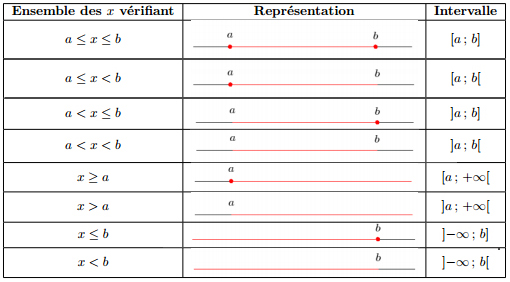
\includegraphics[scale=0.7]{cours4.jpg}
\end{center}


\EPC{1}{FEA-5}{Représenter}

\mini{
\EPC{1}{FEA-16}{Représenter}
}{
\EPC{0}{FEA-14}{Représenter}
}
\begin{DefT}{Intersection}\index{Ensemble!Intersection}
L'\textbf{intersection} de deux ensembles $A$ et $B$ est l'ensemble $A \cap B$ qui contient tous les éléments communs aux deux ensembles.
\end{DefT}

\begin{Rq}\index{Ensembles disjoints}
Deux ensembles sont disjoints lorsque $A \cap B = \oslash$. $\oslash$ est l'ensemble vide.\index{Ensemble!vide}
\end{Rq}


\begin{DefT}{Réunion}\index{Ensemble!Réunion}
La réunion de deux ensembles est l'ensemble $A \cup B$ qui contient tous les éléments des deux ensembles pris une seule fois.
\end{DefT}

\mini{
\EPC{1}{FEA-12}{Représenter}

}{
\EPC{0}{FEA-13}{Représenter}

}

\EPC{1}{FEA-93}{Représenter}

\EPC{0}{FEA-94}{Modéliser}

\EPCP{1}{FEA-92}{Représenter}

\EPC{1}{FEA-83}{Représenter. Chercher.}

\EPC{0}{FEA-83bis}{Représenter. Chercher.}

\paragraphe{Pour s'entrainer en autonomie}

\mini{

\EPC{0}{FEA-16B}{Représenter. Raisonner. Communiquer.}
}{

\EPC{0}{FEA-14B}{Représenter. Raisonner. Communiquer.}
 
}


\mini{

 
\EPC{0}{FEA-12B}{Représenter. Raisonner. Communiquer.}
 
}{

 
\EPC{0}{FEA-13B}{Représenter. Raisonner. Communiquer.}
 
}


\EPC{0}{FEA-108}{Représenter. Communiquer.}

 









% Intervalles de R
%%%\begin{titre}[Les nombres]

\TitreSansTemps{Intervalles de $\R$}{3}
\end{titre}
  
 
 
\EPC{0}{FEA-14_cor}{Représenter}
 
\EPC{0}{FEA-13_cor}{Représenter}

 

\EPC{0}{FEA-94_cor}{Modéliser}

 

\EPC{0}{FEA-83bis_cor}{Représenter. Chercher.}

 
 
 

\EPC{0}{FEA-14B_cor}{Représenter. Raisonner. Communiquer.}
 
============================

 
\EPC{0}{FEA-12B_cor}{Représenter. Raisonner. Communiquer.}
 
 

 
\EPC{0}{FEA-13B}{Représenter. Raisonner. Communiquer.}
 
 


\EPC{0}{FEA-108}{Représenter. Communiquer.}

 










%%
%\begin{titre}[Fonctions et expressions algébriques]

\Titre{Notion de fonction}{4}
\end{titre}


\begin{CpsCol}
\begin{description}
\item[$\square$] Relier représentation graphique et tableau de variations.
\end{description}
\end{CpsCol}



\begin{DefT}{Fonction} \index{Fonction!Antécédent}\index{Fonction!}\index{Fonction!Ensemble de définition}

\begin{minipage}{0.48\linewidth}
Définir une fonction $f$ d'un ensemble D de réels dans $\R$, c'est associer à chaque réel $x$ de D un
unique réel noté $f(x)$.
\begin{description}
\item On dit que D est l'\textbf{ensemble de définition} de $f$. 
\item $f(x)$ est l'\textbf{image} de $x$ par $f$.
\item $x$ est un \textbf{antécédent} de $f(x)$ par $f$.
\end{description}
\end{minipage}
\begin{minipage}{0.48\linewidth}
\begin{center}
\definecolor{sqsqsq}{rgb}{0.12549019607843137,0.12549019607843137,0.12549019607843137}
\definecolor{ffqqqq}{rgb}{1.,0.,0.}
\begin{tikzpicture}[line cap=round,line join=round,>=triangle 45,x=1.0cm,y=1.0cm]
\clip(1.84,4.9) rectangle (9.52,7.);
\draw [color=ffqqqq] (4.,6.62)-- (7.,6.62);
\draw [color=ffqqqq] (7.,6.62)-- (7.,5.32);
\draw [color=ffqqqq] (7.,5.32)-- (4.,5.32);
\draw [color=ffqqqq] (4.,5.32)-- (4.,6.62);
\draw [->] (2.62,6.) -- (4.,6.);
\draw [->] (7.,5.98) -- (8.3,6.);
\draw [color=sqsqsq](2.44,6.25) node[anchor=north west] {|};
\draw [color=sqsqsq](4.58,6.2) node[anchor=north west] {fonction};
\draw [color=sqsqsq](6.34,6.2) node[anchor=north west] {$f$};
\draw [color=sqsqsq](2.06,6.2) node[anchor=north west] {$x$};
\draw [color=sqsqsq](8.36,6.2) node[anchor=north west] {$f(x)$};
\end{tikzpicture}
\end{center}
\end{minipage}
\end{DefT}
 
\begin{Nt}
$f : D \longrightarrow \R$

$x \mapsto f(x)$

Ce qui se lit : la fonction $f$ qui à $x$ associe $f(x)$.
\end{Nt}

\begin{Mt}[Déterminer algébriquement une image, un antécédent par $f$]
Soit $f$ la fonction suivante :

$f$ : $[-4 ; 5] \longrightarrow \R$

$x \mapsto 2x^2 - 6x + 3$.

\begin{description}
\item Pour déterminer l'image d'un nombre $x$ par $f$, il faut que ce nombre soit dans l'ensemble de définition de $f$. Dans ce cas, on remplace $x$ par ce nombre dans l'expression de $f(x)$.

Image de -2 : $f(-2) = 2 \times (-2)^2 -6 \times (-2) + 3 = 2 \times 4 + 12 + 3 = 8 + 12 + 3 = 23$

Image de 6 : Impossible car 6 n'appartient pas à $[-4 ; 5]$.

\item  Pour déterminer le (ou les) antécédent(s) d'un nombre $a$ par $f$, il faut et il suffit de résoudre l'équation $f(x) = 3$.

$2x^2 - 6x + 3 = 3$

$2x^2 - 6x = 0$

$2x (x - 3) = 0$

$2x = 0$ ou $x - 3 = 0$ , $x = 0$ ou  $x = 3$. $\mathscr{S}=\left\lbrace 0;3\right\rbrace $. Les antécédents de 3 par $f$ sont 0 et 3.
\end{description}
\end{Mt}




\EPC{1}{FEA-60}{Calculer. Communiquer}

\mini{
\EPC{0}{FEA-60bis}{Calculer. Communiquer}
}{
\EPC{1}{FEA-46}{Chercher. Calculer.}
}


\EPC{1}{FEA-107}{Calculer. Communiquer}

\mini{
\EPC{1}{FEA-48}{Raisonner. Communiquer}
}{

\EPC{1}{FEA-50}{Modéliser. Calculer}

\EPC{1}{FEA-61}{Raisonner. Communiquer}

\EPC{0}{FEA-45}{Raisonner. Calculer}
}


 
\EPC{0}{FEA-53}{Calculer}
 

\begin{Rqs}
\begin{description}
\item[•] Une fonction peut être donnée, sur un ensemble de définition $D$, par une \textbf{formule algébrique}, un \textbf{tableau de valeurs}, une \textbf{courbe}. 
\item[•] Le seul mode de définition qui permet le calcul d'images et d'antécédents est la formule algébrique. La courbe est imité par la précision et le tableau de valeur par le nombre de valeurs proposées.
\end{description}
\end{Rqs}


\EPCP{1}{FEA-109}{Calculer}


\end{pageCours}

\begin{pageAD}


\begin{ExoCad}{Représenter. Chercher.}{1234}{2}{0}{0}{0}{0}
 
Soit $A$ et $B$ d'abscisse respective $4$ et $-2$.

\begin{enumerate}
\item Le point $I$ est le milieu de $[AB]$. Quelle est l'abscisse du point $I$ ? 
\item Soit $M$ le point d'abscisse $x$ de la droite $(AB)$. Calculer $IM$. 
\item Compléter le tableau suivant.

\begin{tabular}{|c|p{1.5cm}|c|p{1.5cm}|c|p{1.5cm}|}
\hline 
Abscisses de $M$ & $IM$ & Abscisses de $M$ & $IM$ & Abscisses de $M$ & $IM$ \\ 
\hline 
$1$ & & $-6$ &  & $-1$ & \\ 
\hline 
$-2$ & & $3$ &  & $1$ & \\ 
\hline 
$5$ & & $0$ &  & $4$ & \\ 
\hline 
\end{tabular}

\item  A quelle condition le point $M$ appartient-il au segment $[AB]$ ?

\end{enumerate}

On pourra se rendre à la page Se rendre à la page : \url{https://www.geogebra.org/m/jsvqnzbq} pour visualiser la situation. 
\end{ExoCad}
 

\begin{ExoCad}{Chercher. Communiquer.}{1234}{2}{0}{0}{0}{0}

 
\begin{enumerate}
\item Soit $A$ et $B$ d'abscisse respective $3$ et $-1$. Déterminer le rayon de l'intervalle $[AB]$.
\item Représenter le segment $[AB]$ par un intervalle puis par une inégalité.

\item Représenter sur la droite graduée le segment $[AB]$.
 
\end{enumerate}
  
\end{ExoCad}


 
 
\begin{ExoCad}{Représenter. Chercher.}{1234}{2}{0}{0}{0}{0}

On donne les segments $[AB]$ et $[EF]$ représentés ci-dessous.

\definecolor{ttqqqq}{rgb}{0.2,0.,0.}
\definecolor{qqzzff}{rgb}{0.,0.6,1.}
\definecolor{qqzzcc}{rgb}{0.,0.6,0.8}
\begin{tikzpicture}[line cap=round,line join=round,>=triangle 45,x=1.0cm,y=1.0cm]
\begin{axis}[
x=1.0cm,y=1.0cm,
axis lines=middle,
xmin=-2.200000000000002,
xmax=8.480000000000008,
ymin=-0.8000000000000048,
ymax=0.7799999999999957,
xtick={-2.0,-1.0,...,8.0},
ytick={-0.0,1.0,...,0.0},]
\clip(-2.2,-0.8) rectangle (8.48,0.78);
\draw [line width=2.pt,color=qqzzff] (-2.,0.)-- (4.,0.);
\draw [line width=2.pt] (5.,0.)-- (8.,0.);
\begin{scriptsize}
\draw [color=qqzzcc] (-2.,0.)-- ++(-2.5pt,0 pt) -- ++(5.0pt,0 pt) ++(-2.5pt,-2.5pt) -- ++(0 pt,5.0pt);
\draw[color=qqzzcc] (-1.86,0.37) node {$A$};
\draw [color=qqzzcc] (4.,0.)-- ++(-2.5pt,0 pt) -- ++(5.0pt,0 pt) ++(-2.5pt,-2.5pt) -- ++(0 pt,5.0pt);
\draw[color=qqzzcc] (3.96,0.37) node {$B$};
\draw [color=ttqqqq] (5.,0.)-- ++(-2.5pt,0 pt) -- ++(5.0pt,0 pt) ++(-2.5pt,-2.5pt) -- ++(0 pt,5.0pt);
\draw[color=ttqqqq] (5.14,0.37) node {$E$};
\draw [color=ttqqqq] (8.,0.)-- ++(-2.5pt,0 pt) -- ++(5.0pt,0 pt) ++(-2.5pt,-2.5pt) -- ++(0 pt,5.0pt);
\draw[color=ttqqqq] (8.14,0.37) node {$F$};
\end{scriptsize}
\end{axis}
\end{tikzpicture}


\begin{enumerate}
\item 
	\begin{enumerate}
		\item Déterminer le rayon de l'intervalle $[AB]$.
		\item Représenter $[AB]$ par une inégalité.
	\end{enumerate}
\item 
	\begin{enumerate}
		\item Déterminer le rayon de l'intervalle $[EF]$.
		\item Représenter $[EF]$ par une inégalité.
	\end{enumerate}
\end{enumerate}
 
\end{ExoCad}

\begin{ExoCad}{Représenter. Chercher.}{1234}{2}{0}{0}{0}{0}

Soit $x$ un réel.   


\begin{enumerate}
	\item Déterminer puis représenter l'ensemble des points $M$ d'abscisse $x$ tel que $\vert x- 3 \vert \leq 3$.
	\item Déterminer puis représenter l'ensemble des points $M$ d'abscisse $x$ tel que $\vert x+4 \vert \leq 1$.
	\item Déterminer puis représenter l'ensemble des points $M$ d'abscisse $x$ tel que $\vert x+\frac{2}{3} \vert \leq 4$.
\end{enumerate}
 
\end{ExoCad}

\begin{ExoCad}{Représenter. Chercher.}{1234}{2}{0}{0}{0}{0}

Soit $x$ un réel.   


\begin{enumerate}
	\item Déterminer puis représenter l'ensemble des points $M$ d'abscisse $x$ tel que $\vert x - \frac{4}{5} \vert \leq \frac{1}{2}$.
    \item Déterminer puis représenter l'ensemble des points $M$ d'abscisse $x$ tel que $\vert x- \pi \vert \leq 1$.
	\item Déterminer puis représenter l'ensemble des points $M$ d'abscisse $x$ tel que $\vert x - \sqrt{2}  \vert \leq  1$.
	\item Écrire à l'aide d'une double inégalité puis représenter  l'ensemble tel  que $\vert x + \frac{2}{3} \vert \leq 5$.
	\item Écrire à l'aide d'une double inégalité puis représenter  l'ensemble tel  que $\vert x+ \pi \vert \leq 10^{-1}$.	
\end{enumerate}
 
\end{ExoCad}

\begin{ExoCad}{Représenter. Chercher.}{1234}{2}{0}{0}{0}{0}

\begin{enumerate}
\item On s'intéresse à $\frac{3}{7}$.
\begin{enumerate}
	\item 1 est-elle une valeur approchée de $\frac{3}{7}$ à $ 10^{-1}$ près ?
	\item Déterminer une valeur approchée $a$ à $ 10^{-1}$ près de $\frac{3}{7}$.	
\end{enumerate}

\item
On s'intéresse à $\sqrt{10}$.
\begin{enumerate}
	\item Déterminer un encadrement de $\sqrt{10}$ à $ 10^{-2}$ près .
	\item Déterminer à la calculatrice  une valeur approchée de  $\sqrt{10}$.	
\end{enumerate}
\end{enumerate}
  
\end{ExoCad}


\end{pageAD}

%%%%%%%%%%%%%%%%%%%%%%%%%%%%%%%%%%%%%%%%%%%%%%%%%%%%%%%%%%%%%%%%%%%%%%%%%%%%%%%%%%%%%%%%%%%%%%%%%%%%%%%%%%%%%%%%%%%%%%%%%%%
%%%%%%%%%%%%%%%%%%%%%%%%%%%%%%%%%%%%%%%%%%%%%%%%%%%%%%%%%%%%%%%%%%%%%%%%%%%%%%%%%%%%%%%%%%%%%%%%%%%%%%%%%%%%%%%%%%%%%%%%%%%
%%%%%%%%%%%%%%%              pageParcoursu                         %%%%%%%%%%%%%%%%%%%%%%%%%%%%%%%%%%%%%%%%%%%%%%%%%%%%%%%%
%%%%%%%%%%%%%%%%%%%%%%%%%%%%%%%%%%%%%%%%%%%%%%%%%%%%%%%%%%%%%%%%%%%%%%%%%%%%%%%%%%%%%%%%%%%%%%%%%%%%%%%%%%%%%%%%%%%%%%%%%%%
%%%%%%%%%%%%%%%%%%%%%%%%%%%%%%%%%%%%%%%%%%%%%%%%%%%%%%%%%%%%%%%%%%%%%%%%%%%%%%%%%%%%%%%%%%%%%%%%%%%%%%%%%%%%%%%%%%%%%%%%%%%
\begin{pageParcoursu}

\begin{ExoCu}{Représenter. Chercher.}{1234}{2}{0}{0}{0}{0}
 
\end{ExoCu}

\begin{ExoCu}{Représenter. Chercher.}{1234}{2}{0}{0}{0}{0}
 
\end{ExoCu}

\begin{ExoCu}{Représenter. Chercher.}{1234}{2}{0}{0}{0}{0}
 
\end{ExoCu}


\end{pageParcoursu}
%%%%%%%%%%%%%%%%%%%%%%%%%%%%%%%%%%%%%%%%%%%%%%%%%%%%%%%%%%%%%%%%%%%%%%%%%%%%%%%%%%%%%%%%%%%%%%%%%%%%%%%%%%%%%%%%%%%%%%%%%%%
%%%%%%%%%%%%%%%%%%%%%%%%%%%%%%%%%%%%%%%%%%%%%%%%%%%%%%%%%%%%%%%%%%%%%%%%%%%%%%%%%%%%%%%%%%%%%%%%%%%%%%%%%%%%%%%%%%%%%%%%%%%
%%%%%%%%%%%%%%%              pageParcoursd                    %%%%%%%%%%%%%%%%%%%%%%%%%%%%%%%%%%%%%%%%%%%%%%%%%%%%%%%%%%%%%
%%%%%%%%%%%%%%%%%%%%%%%%%%%%%%%%%%%%%%%%%%%%%%%%%%%%%%%%%%%%%%%%%%%%%%%%%%%%%%%%%%%%%%%%%%%%%%%%%%%%%%%%%%%%%%%%%%%%%%%%%%%
%%%%%%%%%%%%%%%%%%%%%%%%%%%%%%%%%%%%%%%%%%%%%%%%%%%%%%%%%%%%%%%%%%%%%%%%%%%%%%%%%%%%%%%%%%%%%%%%%%%%%%%%%%%%%%%%%%%%%%%%%%%

\begin{pageParcoursd}

\begin{ExoCd}{Représenter. Chercher.}{1234}{2}{0}{0}{0}{0}
 
\end{ExoCd}

\begin{ExoCd}{Représenter. Chercher.}{1234}{2}{0}{0}{0}{0}
 
\end{ExoCd}

\begin{ExoCd}{Représenter. Chercher.}{1234}{2}{0}{0}{0}{0}
 
\end{ExoCd}


\end{pageParcoursd}

%%%%%%%%%%%%%%%%%%%%%%%%%%%%%%%%%%%%%%%%%%%%%%%%%%%%%%%%%%%%%%%%%%%%%%%%%%%%%%%%%%%%%%%%%%%%%%%%%%%%%%%%%%%%%%%%%%%%%%%%%%%
%%%%%%%%%%%%%%%%%%%%%%%%%%%%%%%%%%%%%%%%%%%%%%%%%%%%%%%%%%%%%%%%%%%%%%%%%%%%%%%%%%%%%%%%%%%%%%%%%%%%%%%%%%%%%%%%%%%%%%%%%%%
%%%%%%%%%%%%%%%            pageParcourst                      %%%%%%%%%%%%%%%%%%%%%%%%%%%%%%%%%%%%%%%%%%%%%%%%%%%%%%%%%%%%%
%%%%%%%%%%%%%%%%%%%%%%%%%%%%%%%%%%%%%%%%%%%%%%%%%%%%%%%%%%%%%%%%%%%%%%%%%%%%%%%%%%%%%%%%%%%%%%%%%%%%%%%%%%%%%%%%%%%%%%%%%%%
%%%%%%%%%%%%%%%%%%%%%%%%%%%%%%%%%%%%%%%%%%%%%%%%%%%%%%%%%%%%%%%%%%%%%%%%%%%%%%%%%%%%%%%%%%%%%%%%%%%%%%%%%%%%%%%%%%%%%%%%%%%

\begin{pageParcourst}

\begin{ExoCt}{Représenter. Chercher.}{1234}{2}{0}{0}{0}{0}
 
\end{ExoCt}

\begin{ExoCt}{Représenter. Chercher.}{1234}{2}{0}{0}{0}{0}
 
\end{ExoCt}

\begin{ExoCt}{Représenter. Chercher.}{1234}{2}{0}{0}{0}{0}
 
\end{ExoCt}


\end{pageParcourst}
%%%%%%%%%%%%%%%%%%%%%%%%%%%%%%%%%%%%%%%%%%%%%%%%%%%%%%%%%%%%%%%%%%%%%%%%%%%%%%%%%%%%%%%%%%%%%%%%%%%%%%%%%%%%%%%%%%%%%%%%%%%
%%%%%%%%%%%%%%%%%%%%%%%%%%%%%%%%%%%%%%%%%%%%%%%%%%%%%%%%%%%%%%%%%%%%%%%%%%%%%%%%%%%%%%%%%%%%%%%%%%%%%%%%%%%%%%%%%%%%%%%%%%%
%%%%%%%%%%%%%%%              pageAuto                         %%%%%%%%%%%%%%%%%%%%%%%%%%%%%%%%%%%%%%%%%%%%%%%%%%%%%%%%%%%%%
%%%%%%%%%%%%%%%%%%%%%%%%%%%%%%%%%%%%%%%%%%%%%%%%%%%%%%%%%%%%%%%%%%%%%%%%%%%%%%%%%%%%%%%%%%%%%%%%%%%%%%%%%%%%%%%%%%%%%%%%%%%
%%%%%%%%%%%%%%%%%%%%%%%%%%%%%%%%%%%%%%%%%%%%%%%%%%%%%%%%%%%%%%%%%%%%%%%%%%%%%%%%%%%%%%%%%%%%%%%%%%%%%%%%%%%%%%%%%%%%%%%%%%%
\begin{pageAuto}

\begin{ExoAuto}{Représenter. Chercher.}{1234}{2}{0}{0}{0}{0}
 
\end{ExoAuto}

\begin{ExoAuto}{Représenter. Chercher.}{1234}{2}{0}{0}{0}{0}
 
\end{ExoAuto}

\begin{ExoAuto}{Représenter. Chercher.}{1234}{2}{0}{0}{0}{0}
 
\end{ExoAuto}


\end{pageAuto} % Ensemble de définition et variables, Image et antécédent
\begin{titre}[Informations chiffrées]

\Titre{Taux d'évolution}{4}
\end{titre}


\begin{CpsCol}
\begin{description}
\item[$\square$] Exploiter la relation entre deux valeurs successives et leur taux d’évolution.
\end{description}
\end{CpsCol}

\EPC{1}{IC-41}{Modéliser. Calculer.}

\begin{DefT}{Variation absolue, relative}\index{Variation absolue}\index{Variation relative, Taux d'évolution}
On considère une quantité qui varie et on appelle $V_i$ sa valeur initiale et $V_f$ sa valeur finale. 
La \textbf{variation absolue} $\Delta V$ est donnée par : $\Delta V = V_f - V_i$.

La \textbf{variation relative} ou \textbf{taux d'évolution $t$} est donnée par : $t = \frac{V_f - V_i}{V_i}$.
\end{DefT}

\begin{Ex}
Paul place 110 euros sur son compte. Il se rend compte 15 jours plus tard qu'il possède 121 euros sur son compte.

La variation absolue est $\Delta V = 121 - 110 = +11$ euros.

La variation relative est $t = \frac{121 - 110}{110}=\frac{11}{110}= +10\%$.
\end{Ex}


%%%%%%% Exercices



\begin{DefT}{Taux d'évolution}\index{Taux d'évolution}

 Soit $t$ le \textbf{taux d'évolution} qui permet à une quantité de passer de $V_i$ à $V_f$.
 On a alors : $V_f = (1+t) \times V_i$.
\end{DefT}

 
\begin{DefT}{Coefficient multiplicateur}
 
Le réel $1+t$ est appelé \textbf{coefficient multiplicateur} associé au taux $t$. On peut le noter $CM$. Avec cette notation, on a alors  $V_f = CM \times V_i$ où $CM =1+t$. 
\end{DefT}

\EPC{1}{IC-2}{Calculer.}


\begin{minipage}{0.58\linewidth}
\begin{Th} 

Soit $CM$ le coefficient multiplicateur et $t$ le taux d'évolution, $t =CM-1$. 
\end{Th}
\end{minipage}
\hfill
\begin{minipage}{0.38\linewidth}

\begin{Rq} 
Pour $V_i \neq 0$, $CM=\frac{V_f}{V_i}$ . 
\end{Rq}
\end{minipage}


\begin{Th} 
\begin{description}
\item[•] Dans le cas d'une baisse, le taux d'évolution est négatif et le $CM$ est compris entre 0 et 1.
\item[•] Dans le cas d'une hausse, le taux d'évolution est positif et le $CM$ est supérieur à 1.
\end{description}

 
\end{Th}

%Exercices




\mini{
\EPC{1}{IC-27}{Calculer.}  

\EPC{1}{IC-28}{Raisonner.}

\EPC{1}{IC-29}{Modéliser. Calculer.}

\EPC{0}{IC-24}{Modéliser. Calculer.} 

}{
\EPC{1}{IC-25}{Modéliser. Calculer.} 

\EPC{0}{IC-26}{Raisonner. Calculer.} 

\EPC{1}{IC-30}{Raisonner. Calculer.}


\EPC{1}{IC-31}{Modéliser. Calculer.} 
}


 

\EPC{0}{IC-1}{Raisonner. Modéliser. Calculer.} % Taux d'évolutions
%%%%%%\begin{titre}[Les statistiques]

{\color{bleu3}{\LARGE Utilisation d'un tableur} \hfill{Niveau 1}}
\end{titre}



\begin{CpsCol}
\textbf{Interpréter, représenter et traiter des données}
\begin{description}
\item[$\square$] Calculer une fréquence
\item[$\square$] Utiliser un tableur pour effectuer des calcul
\end{description}
\end{CpsCol}

\begin{Rec}

Le travail de statistiques est souvent fastidieux, on a toujours recours à un tableur lorsque les données sont trop importantes. Une feuille de calcul d'un tableur se présente comme cela, en cellules. La cellule rouge est la cellule C3.

L'intérêt d'un tableur est le calcul automatique des caractéristiques demandées : moyenne, fréquence, effectif cumulés,... Pour cela, il faut utiliser des formules mathématiques.

\vspace{0.4cm}

\begin{tabular}{|c|m{2cm}|m{2cm}|m{2cm}|m{2cm}|m{2cm}|}
\hline 
\rowcolor{gray} & A & B & C & D &...\\ 
\hline 
\cellcolor{gray}1 & &4 &  & &  \\ 
\hline 
\cellcolor{gray}2 & & & 5 & &   \\ 
\hline 
\cellcolor{gray}3 & & & \cellcolor{red} & &  \\ 
\hline 
\cellcolor{gray}... & & &  & & \\ 
\hline 
\end{tabular} 

\subsubsection*{Quelques formules : Utilisation du signe = avant toute formule}

\begin{description}
\item[=a+b] calcule la somme de  $a$ et de $b$. 
\item[=SOMME(plage)] calcule la somme des cellules dans une plage rectangulaire.
\item[=NB.SI(plage;critère] renvoie parmi les cellules de la plage celle qui vérifie le critères.
\item[=a/b] calcule le quotient de  $a$ par $b$. $b$ doit être non nul.
\end{description}

\subsubsection*{Utilisations}
\begin{description}[leftmargin=*]
\item Pour calculer 4+5 dans la cellule D3, on tapera dans la cellule D3, \textbf{=B1+C2}. Lorsque une des valeurs des cellules B1 ou C2 change, la somme change alors. 
\item Pour calculer 4/5 dans la cellule B3, on tapera dans la cellule DB3, \textbf{=B1/C2}. 
\end{description}

\subsection*{Application concrète}

Voici les notes obtenues à un contrôle sur 10 par une classe de quatrième :\\
0 -- 1 -- 2 -- 2 -- 3 -- 3 -- 3 -- 3 -- 4 -- 4 -- 5 -- 5 -- 5 -- 6 -- 6 -- 6 -- 7 -- 7 -- 8 -- 8 -- 8 -- 9 -- 9 -- 10 -- 10.

\begin{enumerate}
\item Créer un tableau sur une feuille de calcul et complète le tableau ci-dessous avec les formules adéquates.
\item Combien d'élèves ont obtenu moins de 5 ?
\item Quel est le pourcentage d'élèves qui ont obtenu 8 ?
\item Quel est le pourcentage d'élèves qui ont obtenu au moins 8 ?
\item Change un 3 et par un 8 dans la série statistique. Remarque le changement de résultats.
\end{enumerate}

\begin{tabular}{|p{4.2cm}*{11}{|p{5mm}}|p{8mm}|}
\hline
Note&0 & 1 & 2& 3 & 4 & 5 & 6&7 &8 &9 &10&Total \\
\hline
Effectifs&1 & 1 & 2& &&&& & &&& \\
\hline
Effectifs cumulés&1 & 2 & 4& &  & & & && & & \\
\hline
Fréquences &0,04 & 0,04 & 0,08 & &  & & & & & & & \\
\hline
Fréquences cumulées &0,04  & 0,08  & 0,16  &  &  & & & & & & & \\
\hline
\end{tabular}




\subsubsection*{Effectifs -- Effectifs cumulés}
	Pour chaque note, {\em l'effectif} est le nombre d'élèves ayant eu cette note.	Par exemple (dans le tableau), 1 élève a eu 0 ;	2 élèves ont eu 1\dots\\ 
	Pour chaque note, {\em l'effectif cumulé} est le nombre d'élèves ayant eu cette note ou une note inférieure. Pour le calculer, il suffit à chaque fois de cumuler les effectifs.\\
	Par exemple (dans le tableau), 1 élève a eu 0 ;	$1+2=3$ élèves ont eu 1 au plus ; $3+4=7$ élèves ont eu 2 au plus\dots
	
\subsubsection*{Fréquences -- Fréquences cumulées}
	Pour chaque note, {\em la fréquence} exprime la proportion d'élèves. Par exemple, sur les 20 élèves, 4 élèves ont eu une note de 2.
	La proportion est de 4 sur 20 ou $4\over20$ que l'on exprime en \%\ par le calcul $100\times{4\over20}=20$.\\
	Comme pour les effectifs cumulés, les {\em fréquences cumulées}	sont obtenues en cumulant les fréquences.
\end{Rec}

\begin{DefT}{Fréquence}
La population $P$ étudiée a un effectif total égal à $N$.
La fréquence $f$ d'un sous ensemble de la population, appelé $A$, d'effectif $n$ est le quotient de cet effectif sur l'effectif total $N$. On écrit alors $f_A=\frac{n}{N}$.
\end{DefT}


\begin{Ex}
Une classe de Quatrième compte 25 élèves dont 12 filles.\\
La population est l'ensemble des élèves de la classe. L'effectif de la population est égal à 25, c'est l'effectif total : $N=25$.\\
Pour calculer la fréquence des filles dans cette classe, on détermine l'effectif de ce sous ensemble : les filles. $n=12$\\
Donc $f_{filles}=\frac{12}{25}$.
\end{Ex}

\begin{AD}

Lors du concours Algoréa, les 12\% meilleurs élèves sont qualifiés pour le tour suivant. 
\begin{description}
\item[•] En sixième, Mathis est arrivée $682^{ième}$ sur 6800 participants.
\item[•] En cinquième, Pol est arrivé $524^{ième}$ sur 5200 participants.
\item[•] En quatrième, Luisa est arrivée $855^{ième}$ sur 8200 participants.
\item[•] En troisième, Rafaela est arrivée $423^{ième}$ sur 4500 participants.
\end{description}
Quel élèves ont été sélectionnés pour le tour suivant ?

\end{AD}


\begin{AD}

Lors de la première édition de la Course aux Nombres, les 24 élèves de la classe de Cinquième 2 en Colombie ont obtenu les résultats suivants. Les notes sont évaluées sur 30 points.


\begin{enumerate}
\item Reproduire la feuille de calcul comme indiqué ci dessous.

\begin{tabular}{|c|c|c|c|c|c|c|c|c|c|}
\hline 
\rowcolor{gray} & A & B & C & D & E & F & G & H & I \\ 
\hline 
\cellcolor{gray} 1 & 11 & 16 & 22 & 20 & 26 &  &  & Nombres d'élèves total &  \\ 
\hline 
\cellcolor{gray}2& 26 & 18 & 26 & 19& 16 &  &  & Nombre d'élèves dont la nombre est égale à 22 &  \\ 
\hline 
\cellcolor{gray}3 & 17 &27 & 18 & 16 & 22 &  & & Fréquence d'élèves dont la note est égale à 22 &  \\ 
\hline 
\cellcolor{gray}4 & 16 & 19 & 11 & 21 & 17 & &  & Nombre d'élèves dont la note est égale à 19 &  \\ 
\hline 
\cellcolor{gray}5 & 22 & 15 & 22 & 23 &  &  &  & Fréquence d'élèves dont la note est égale à 19 &  \\ 
\hline 
\end{tabular} 

\item  
\begin{enumerate}
\item  Déterminer dans la cellule I1 le nombre d'élèves participants à ce jeu. 
Rappel : Pour déterminer le nombre de cases remplies d'un tableau, on utilise la syntaxe : =NB(A1:E5). 
\item  Déterminer dans la cellule I2 le nombre d'élèves dont la note est égale à 22 ? 
Rappel : Pour déterminer le nombre de cases remplies avec la valeur 22, on utilise la syntaxe : =NB.SI(A1:E5;22). 
\item  Calcule dans la cellule I3 la fréquence des élèves ayant obtenu 22.
\end{enumerate}
\item  
\begin{enumerate}
\item Détermine la moyenne de cette classe. On pourra utiliser la syntaxe "=MOYENNE(A1:E5)".
\item Explique par une phrase le calcul du tableur pour donner la moyenne.
\item 
\begin{enumerate}
\item Complète le tableau ci-dessous.

\begin{tabular}{|c|c|c|c|c|c|c|}
\hline 
Notes & $[0;5[$ &  $[5;10[$  &  $[10;15[$  &  $[15;20[$  &  $[20;25[$  &  $[25;30]$  \\ 
\hline 
Fréquence &  &  &  &  &  &  \\ 
\hline 
\end{tabular} 

\item Calcule la moyenne avec ce regroupement.	
\end{enumerate}
\item Création d'un diagramme avec un tableur
\begin{enumerate}
\item  Sélectionne la plage de données A1:E5 puis clique sur l'icône graphique
\item  Quel est le problème de la plage de données A1:E5 ?
\end{enumerate}

\end{enumerate}
\end{enumerate}




\end{AD}


\begin{autoeval}
\begin{tabular}{p{12cm}p{0.5cm}p{0.5cm}p{0.5cm}p{1cm}}
\textbf{Compétences visées} &  M I & MF & MF  & TBM \vcomp \\ 
Calculer une fréquence & $\square$ & $\square$  & $\square$ & $\square$ \vcomp \\ 
Utiliser un tableur pour effectuer des calcul & $\square$ & $\square$ & $\square$ & $\square$ \vcomp \\ 
\end{tabular}
{\footnotesize MI : maitrise insuffisante ; MF = Maitrise fragile ; MS = Maitrise satisfaisante ; TBM = Très bonne maitrise}
 
\end{autoeval} % Effectifs cumulés, fréquences cumulées 
%\begin{titre}[Fonctions et expressions algébriques]

\Titre{Lecture graphique}{4}
\end{titre}


\begin{CpsCol}
\begin{description}
\item[$\square$] Exploiter l’équation $y = f(x)$ d’une courbe : appartenance, calcul de coordonnées.
\item[$\square$] Résoudre une équation ou une inéquation du type $f(x) = k$ ou $f(x) < k$.
\item[$\square$] Résoudre, graphiquement, une équation ou inéquation du type $f(x) = g(x)$ ou $f(x) < g(x)$.
\end{description}
\end{CpsCol}


\Rec{1}{FEA-52}

\begin{DefT}{Représentation graphique}\index{Représentation graphique}\index{Équation de courbe}
Soit $f$ une fonction définie sur l'ensemble $D$.\\
Le plan est muni d'un repère (O ; I ; J).\\
La \textbf{représentation graphique} ou courbe représentative $\mathscr{C}_f$ de la fonction $f$ dans le repère (O ; I ; J) est l'ensemble des points de coordonnées $(x ; f (x))$, où $x \in D$.
Une équation de $\mathscr{C}_f$ est $y=f(x)$.
\end{DefT}

\begin{Pp}[Appartenance d'un point à une courbe]
Un point $A(x_A;y_A)$ appartient à une courbe $\mathscr{C}$ d'équation $y=f(x)$ si et seulement si les coordonnées de $A$ vérifient l'équation de la courbe $\mathscr{C}$. On symbolise par : $ A \in \mathscr{C}  \Longleftrightarrow y_A=f(x_A)$.
\end{Pp}

\begin{Rqs}
\begin{itemize}
\item En général, le repère sera orthogonal ou orthonormal.
\item Le tracé d’une courbe représentative est toujours approximatif : on construit un tableau de valeurs, on place les points correspondants dans un repère et on les relie par une courbe régulière
(sans utiliser la règle, sauf dans certains cas particuliers).
\item On peut utiliser la calculatrice pour remplir un tableau de valeurs et tracer des courbes représentatives. 
\item Certaines fonctions ne sont connues que par leur courbe représentative
\end{itemize}
\end{Rqs}

\begin{Mt}[. Construction de courbe]\index{Construction de courbe}

Soit la fonction $f$ définie sur $\R$ par $f(x)=\frac{4x+3}{x^2+1}$.

$x^2+1 > 0$ donc pour toutes les valeurs de $x$, $f(x)$ existe. 

Donc le domaine de définition est $\R$.

On commence par construire, à l'aide de la calculatrice, un tableau de valeurs. Pour placer des points dans un
repère, des valeurs approchées suffisent.

On place les points correspondants dans le repère choisi, et on les joints par une courbe régulière (voir
figure ci dessous).

\begin{center}
\definecolor{ffqqqq}{rgb}{1.,0.,0.}
\definecolor{qqqqff}{rgb}{0.,0.,1.}
\definecolor{cqcqcq}{rgb}{0.7529411764705882,0.7529411764705882,0.7529411764705882}
\begin{tikzpicture}[line cap=round,line join=round,>=triangle 45,x=1.0cm,y=1.0cm]
\draw [color=cqcqcq,, xstep=0.5cm,ystep=0.5cm] (-4.486899146925993,-1.2029939912205303) grid (7.341764903922375,4.241161011261972);
\draw[->,color=black] (-4.486899146925993,0.) -- (7.341764903922375,0.);
\foreach \x in {-4.,-3.5,-3.,-2.5,-2.,-1.5,-1.,-0.5,0.5,1.,1.5,2.,2.5,3.,3.5,4.,4.5,5.,5.5,6.,6.5,7.}
\draw[shift={(\x,0)},color=black] (0pt,2pt) -- (0pt,-2pt) node[below] {\footnotesize $\x$};
\draw[->,color=black] (0.,-1.2029939912205303) -- (0.,4.241161011261972);
\foreach \y in {-1.,-0.5,0.5,1.,1.5,2.,2.5,3.,3.5,4.}
\draw[shift={(0,\y)},color=black] (2pt,0pt) -- (-2pt,0pt) node[left] {\footnotesize $\y$};
\draw[color=black] (0pt,-10pt) node[right] {\footnotesize $0$};
\clip(-4.486899146925993,-1.2029939912205303) rectangle (7.341764903922375,4.241161011261972);
\draw[line width=1.2pt,color=qqqqff,smooth,samples=100,domain=-4.486899146925993:7.341764903922375] plot(\x,{(4.0*(\x)+3.0)/((\x)^(2.0)+1.0)});
\begin{scriptsize}
\draw[color=qqqqff] (-6.298317993206538,-0.6090861727678938) node {$g$};
\draw [color=ffqqqq] (-1.,-0.5)-- ++(-2.5pt,0 pt) -- ++(5.0pt,0 pt) ++(-2.5pt,-2.5pt) -- ++(0 pt,5.0pt);
\draw [color=ffqqqq] (0.,3.)-- ++(-2.5pt,0 pt) -- ++(5.0pt,0 pt) ++(-2.5pt,-2.5pt) -- ++(0 pt,5.0pt);
\draw [color=ffqqqq] (0.98,3.5298918588043255)-- ++(-2.5pt,0 pt) -- ++(5.0pt,0 pt) ++(-2.5pt,-2.5pt) -- ++(0 pt,5.0pt);
\draw [color=ffqqqq] (1.98,2.2193317616453947)-- ++(-2.5pt,0 pt) -- ++(5.0pt,0 pt) ++(-2.5pt,-2.5pt) -- ++(0 pt,5.0pt);
\draw [color=ffqqqq] (3.,1.5)-- ++(-2.5pt,0 pt) -- ++(5.0pt,0 pt) ++(-2.5pt,-2.5pt) -- ++(0 pt,5.0pt);
\draw [color=ffqqqq] (4.,1.1176470588235294)-- ++(-2.5pt,0 pt) -- ++(5.0pt,0 pt) ++(-2.5pt,-2.5pt) -- ++(0 pt,5.0pt);
\draw [color=ffqqqq] (5.04,0.8772195624507605)-- ++(-2.5pt,0 pt) -- ++(5.0pt,0 pt) ++(-2.5pt,-2.5pt) -- ++(0 pt,5.0pt);
\draw [color=ffqqqq] (6.,0.7297297297297297)-- ++(-2.5pt,0 pt) -- ++(5.0pt,0 pt) ++(-2.5pt,-2.5pt) -- ++(0 pt,5.0pt);
\draw [color=ffqqqq] (7.,0.62)-- ++(-2.5pt,0 pt) -- ++(5.0pt,0 pt) ++(-2.5pt,-2.5pt) -- ++(0 pt,5.0pt);
\draw [color=ffqqqq] (-2.,-1.)-- ++(-2.5pt,0 pt) -- ++(5.0pt,0 pt) ++(-2.5pt,-2.5pt) -- ++(0 pt,5.0pt);
\draw [color=ffqqqq] (-2.98,-0.90279745759281)-- ++(-2.5pt,0 pt) -- ++(5.0pt,0 pt) ++(-2.5pt,-2.5pt) -- ++(0 pt,5.0pt);
\draw [color=ffqqqq] (-4.1,-0.7523862998315552)-- ++(-2.5pt,0 pt) -- ++(5.0pt,0 pt) ++(-2.5pt,-2.5pt) -- ++(0 pt,5.0pt);
\draw [color=ffqqqq] (0.5,4.)-- ++(-2.5pt,0 pt) -- ++(5.0pt,0 pt) ++(-2.5pt,-2.5pt) -- ++(0 pt,5.0pt);
\draw [color=ffqqqq] (-0.5176152269341983,0.7331180540879474)-- ++(-2.5pt,0 pt) -- ++(5.0pt,0 pt) ++(-2.5pt,-2.5pt) -- ++(0 pt,5.0pt);
\draw [color=ffqqqq] (1.50167135580477,2.7670165188890095)-- ++(-2.5pt,0 pt) -- ++(5.0pt,0 pt) ++(-2.5pt,-2.5pt) -- ++(0 pt,5.0pt);
\draw [color=ffqqqq] (-1.5,-0.9230769230769231)-- ++(-2.5pt,0 pt) -- ++(5.0pt,0 pt) ++(-2.5pt,-2.5pt) -- ++(0 pt,5.0pt);
\end{scriptsize}
\end{tikzpicture}
\end{center}
\end{Mt}

\mini{
\EPC{1}{FEA-66}{Représenter. Calculer.}

\EPC{1}{FEA-54}{Représenter. Calculer.}
}{

\EPC{1}{FEA-59}{Représenter. Chercher.}

\EPC{1}{FEA-55}{Représenter.}

\EPC{0}{FEA-67}{Calculer.}

\EPC{0}{FEA-62}{Représenter.}

}


\begin{Mt}[. Déterminer graphiquement une image, un antécédent par $f$]\index{Lecture graphique!Image}\index{Lecture graphique!Antécédent}
On se reportera à la figure ci dessous
\begin{itemize}
\item L’image de $a$ est l’ordonnée du point de la courbe d’abscisse $a$.
\item Les antécédents de $b$ sont les abscisses des points de la courbe dont l’ordonnée est $b$.
\end{itemize}

\begin{minipage}{0.48\linewidth}
\textbf{Lecture d'image}

\definecolor{ffqqqq}{rgb}{1.,0.,0.}
\definecolor{qqwuqq}{rgb}{0.,0.39215686274509803,0.}
\definecolor{uuuuuu}{rgb}{0.26666666666666666,0.26666666666666666,0.26666666666666666}
\definecolor{xdxdff}{rgb}{0.49019607843137253,0.49019607843137253,1.}
\definecolor{ccqqqq}{rgb}{0.8,0.,0.}
\begin{tikzpicture}[line cap=round,line join=round,>=triangle 45,x=1.0cm,y=1.0cm]
\draw[->,color=black] (-1.2,0.) -- (6.54,0.);
\foreach \x in {-1.,1.,2.,3.,4.,5.,6.}
\draw[shift={(\x,0)},color=black] (0pt,2pt) -- (0pt,-2pt) node[below] {\footnotesize $\x$};
\draw[->,color=black] (0.,-0.58) -- (0.,4.1);
\foreach \y in {,1.,2.,3.,4.}
\draw[shift={(0,\y)},color=black] (2pt,0pt) -- (-2pt,0pt) node[left] {\footnotesize $\y$};
\draw[color=black] (0pt,-10pt) node[right] {\footnotesize $0$};
\clip(-1.2,-0.58) rectangle (6.54,4.1);
\draw[line width=1.2pt,color=ccqqqq] (0.02000202000000007,1.0333351288922137) -- (0.02000202000000007,1.0333351288922137);
\draw[line width=1.2pt,color=ccqqqq] (0.02000202000000007,1.0333351288922137) -- (0.0350020088527628,1.0468526628865917);
\draw[line width=1.2pt,color=ccqqqq] (0.0350020088527628,1.0468526628865917) -- (0.050001997705525526,1.0607417842661409);
\draw[line width=1.2pt,color=ccqqqq] (0.050001997705525526,1.0607417842661409) -- (0.06500198655828826,1.075007280091787);
\draw[line width=1.2pt,color=ccqqqq] (0.06500198655828826,1.075007280091787) -- (0.08000197541105099,1.0896537782492035);
\draw[line width=1.2pt,color=ccqqqq] (0.08000197541105099,1.0896537782492035) -- (0.09500196426381372,1.1046857321084331);
\draw[line width=1.2pt,color=ccqqqq] (0.09500196426381372,1.1046857321084331) -- (0.11000195311657644,1.120107404667603);
\draw[line width=1.2pt,color=ccqqqq] (0.11000195311657644,1.120107404667603) -- (0.12500194196933917,1.1359228521975857);
\draw[line width=1.2pt,color=ccqqqq] (0.12500194196933917,1.1359228521975857) -- (0.1400019308221019,1.1521359074080868);
\draw[line width=1.2pt,color=ccqqqq] (0.1400019308221019,1.1521359074080868) -- (0.15500191967486465,1.1687501621594936);
\draw[line width=1.2pt,color=ccqqqq] (0.15500191967486465,1.1687501621594936) -- (0.1700019085276274,1.1857689497488706);
\draw[line width=1.2pt,color=ccqqqq] (0.1700019085276274,1.1857689497488706) -- (0.18500189738039013,1.2031953268027384);
\draw[line width=1.2pt,color=ccqqqq] (0.18500189738039013,1.2031953268027384) -- (0.20000188623315288,1.2210320548137101);
\draw[line width=1.2pt,color=ccqqqq] (0.20000188623315288,1.2210320548137101) -- (0.21500187508591562,1.2392815813626485);
\draw[line width=1.2pt,color=ccqqqq] (0.21500187508591562,1.2392815813626485) -- (0.23000186393867836,1.2579460210727733);
\draw[line width=1.2pt,color=ccqqqq] (0.23000186393867836,1.2579460210727733) -- (0.2450018527914411,1.2770271363470083);
\draw[line width=1.2pt,color=ccqqqq] (0.2450018527914411,1.2770271363470083) -- (0.2600018416442038,1.2965263179448447);
\draw[line width=1.2pt,color=ccqqqq] (0.2600018416442038,1.2965263179448447) -- (0.2750018304969665,1.3164445654600376);
\draw[line width=1.2pt,color=ccqqqq] (0.2750018304969665,1.3164445654600376) -- (0.29000181934972924,1.3367824677655373);
\draw[line width=1.2pt,color=ccqqqq] (0.29000181934972924,1.3367824677655373) -- (0.30500180820249195,1.357540183497144);
\draw[line width=1.2pt,color=ccqqqq] (0.30500180820249195,1.357540183497144) -- (0.32000179705525467,1.3787174216524065);
\draw[line width=1.2pt,color=ccqqqq] (0.32000179705525467,1.3787174216524065) -- (0.3350017859080174,1.4003134223862463);
\draw[line width=1.2pt,color=ccqqqq] (0.3350017859080174,1.4003134223862463) -- (0.3500017747607801,1.422326938089602);
\draw[line width=1.2pt,color=ccqqqq] (0.3500017747607801,1.422326938089602) -- (0.3650017636135428,1.4447562148420192);
\draw[line width=1.2pt,color=ccqqqq] (0.3650017636135428,1.4447562148420192) -- (0.3800017524663055,1.4675989743334903);
\draw[line width=1.2pt,color=ccqqqq] (0.3800017524663055,1.4675989743334903) -- (0.39500174131906823,1.4908523963549363);
\draw[line width=1.2pt,color=ccqqqq] (0.39500174131906823,1.4908523963549363) -- (0.41000173017183095,1.5145131019604348);
\draw[line width=1.2pt,color=ccqqqq] (0.41000173017183095,1.5145131019604348) -- (0.42500171902459366,1.5385771374075912);
\draw[line width=1.2pt,color=ccqqqq] (0.42500171902459366,1.5385771374075912) -- (0.4400017078773564,1.5630399589852422);
\draw[line width=1.2pt,color=ccqqqq] (0.4400017078773564,1.5630399589852422) -- (0.4550016967301191,1.587896418839931);
\draw[line width=1.2pt,color=ccqqqq] (0.4550016967301191,1.587896418839931) -- (0.4700016855828818,1.613140751914209);
\draw[line width=1.2pt,color=ccqqqq] (0.4700016855828818,1.613140751914209) -- (0.4850016744356445,1.6387665641107505);
\draw[line width=1.2pt,color=ccqqqq] (0.4850016744356445,1.6387665641107505) -- (0.5000016632884072,1.6647668217964553);
\draw[line width=1.2pt,color=ccqqqq] (0.5000016632884072,1.6647668217964553) -- (0.51500165214117,1.6911338427600933);
\draw[line width=1.2pt,color=ccqqqq] (0.51500165214117,1.6911338427600933) -- (0.5300016409939328,1.71785928873556);
\draw[line width=1.2pt,color=ccqqqq] (0.5300016409939328,1.71785928873556) -- (0.5450016298466955,1.7449341596004109);
\draw[line width=1.2pt,color=ccqqqq] (0.5450016298466955,1.7449341596004109) -- (0.5600016186994583,1.7723487893559928);
\draw[line width=1.2pt,color=ccqqqq] (0.5600016186994583,1.7723487893559928) -- (0.5750016075522211,1.8000928439911317);
\draw[line width=1.2pt,color=ccqqqq] (0.5750016075522211,1.8000928439911317) -- (0.5900015964049838,1.8281553213259696);
\draw[line width=1.2pt,color=ccqqqq] (0.5900015964049838,1.8281553213259696) -- (0.6050015852577466,1.8565245529261258);
\draw[line width=1.2pt,color=ccqqqq] (0.6050015852577466,1.8565245529261258) -- (0.6200015741105094,1.8851882081698808);
\draw[line width=1.2pt,color=ccqqqq] (0.6200015741105094,1.8851882081698808) -- (0.6350015629632721,1.9141333005425774);
\draw[line width=1.2pt,color=ccqqqq] (0.6350015629632721,1.9141333005425774) -- (0.6500015518160349,1.9433461962228766);
\draw[line width=1.2pt,color=ccqqqq] (0.6500015518160349,1.9433461962228766) -- (0.6650015406687977,1.9728126250149511);
\draw[line width=1.2pt,color=ccqqqq] (0.6650015406687977,1.9728126250149511) -- (0.6800015295215605,2.002517693669182);
\draw[line width=1.2pt,color=ccqqqq] (0.6800015295215605,2.002517693669182) -- (0.6950015183743232,2.0324459016215064);
\draw[line width=1.2pt,color=ccqqqq] (0.6950015183743232,2.0324459016215064) -- (0.710001507227086,2.0625811591682885);
\draw[line width=1.2pt,color=ccqqqq] (0.710001507227086,2.0625811591682885) -- (0.7250014960798488,2.0929068080795825);
\draw[line width=1.2pt,color=ccqqqq] (0.7250014960798488,2.0929068080795825) -- (0.7400014849326115,2.1234056446389857);
\draw[line width=1.2pt,color=ccqqqq] (0.7400014849326115,2.1234056446389857) -- (0.7550014737853743,2.154059945083057);
\draw[line width=1.2pt,color=ccqqqq] (0.7550014737853743,2.154059945083057) -- (0.7700014626381371,2.18485149339765);
\draw[line width=1.2pt,color=ccqqqq] (0.7700014626381371,2.18485149339765) -- (0.7850014514908998,2.215761611412598);
\draw[line width=1.2pt,color=ccqqqq] (0.7850014514908998,2.215761611412598) -- (0.8000014403436626,2.2467711911201036);
\draw[line width=1.2pt,color=ccqqqq] (0.8000014403436626,2.2467711911201036) -- (0.8150014291964254,2.2778607291261768);
\draw[line width=1.2pt,color=ccqqqq] (0.8150014291964254,2.2778607291261768) -- (0.8300014180491881,2.3090103631285572);
\draw[line width=1.2pt,color=ccqqqq] (0.8300014180491881,2.3090103631285572) -- (0.8450014069019509,2.340199910299052);
\draw[line width=1.2pt,color=ccqqqq] (0.8450014069019509,2.340199910299052) -- (0.8600013957547137,2.3714089074331723);
\draw[line width=1.2pt,color=ccqqqq] (0.8600013957547137,2.3714089074331723) -- (0.8750013846074765,2.4026166527156056);
\draw[line width=1.2pt,color=ccqqqq] (0.8750013846074765,2.4026166527156056) -- (0.8900013734602392,2.43380224893654);
\draw[line width=1.2pt,color=ccqqqq] (0.8900013734602392,2.43380224893654) -- (0.905001362313002,2.464944647981332);
\draw[line width=1.2pt,color=ccqqqq] (0.905001362313002,2.464944647981332) -- (0.9200013511657648,2.496022696404641);
\draw[line width=1.2pt,color=ccqqqq] (0.9200013511657648,2.496022696404641) -- (0.9350013400185275,2.527015181890066);
\draw[line width=1.2pt,color=ccqqqq] (0.9350013400185275,2.527015181890066) -- (0.9500013288712903,2.557900880387663);
\draw[line width=1.2pt,color=ccqqqq] (0.9500013288712903,2.557900880387663) -- (0.9650013177240531,2.5886586037145913);
\draw[line width=1.2pt,color=ccqqqq] (0.9650013177240531,2.5886586037145913) -- (0.9800013065768158,2.6192672473986587);
\draw[line width=1.2pt,color=ccqqqq] (0.9800013065768158,2.6192672473986587) -- (0.9950012954295786,2.649705838540742);
\draw[line width=1.2pt,color=ccqqqq] (0.9950012954295786,2.649705838540742) -- (1.0100012842823414,2.6799535834700716);
\draw[line width=1.2pt,color=ccqqqq] (1.0100012842823414,2.6799535834700716) -- (1.0250012731351041,2.709989914966185);
\draw[line width=1.2pt,color=ccqqqq] (1.0250012731351041,2.709989914966185) -- (1.040001261987867,2.7397945388229794);
\draw[line width=1.2pt,color=ccqqqq] (1.040001261987867,2.7397945388229794) -- (1.0550012508406297,2.769347479533794);
\draw[line width=1.2pt,color=ccqqqq] (1.0550012508406297,2.769347479533794) -- (1.0700012396933924,2.798629124881675);
\draw[line width=1.2pt,color=ccqqqq] (1.0700012396933924,2.798629124881675) -- (1.0850012285461552,2.8276202692260393);
\draw[line width=1.2pt,color=ccqqqq] (1.0850012285461552,2.8276202692260393) -- (1.100001217398918,2.8563021552855856);
\draw[line width=1.2pt,color=ccqqqq] (1.100001217398918,2.8563021552855856) -- (1.1150012062516808,2.8846565142276255);
\draw[line width=1.2pt,color=ccqqqq] (1.1150012062516808,2.8846565142276255) -- (1.1300011951044435,2.912665603885687);
\draw[line width=1.2pt,color=ccqqqq] (1.1300011951044435,2.912665603885687) -- (1.1450011839572063,2.940312244940369);
\draw[line width=1.2pt,color=ccqqqq] (1.1450011839572063,2.940312244940369) -- (1.160001172809969,2.9675798549126813);
\draw[line width=1.2pt,color=ccqqqq] (1.160001172809969,2.9675798549126813) -- (1.1750011616627318,2.994452479834413);
\draw[line width=1.2pt,color=ccqqqq] (1.1750011616627318,2.994452479834413) -- (1.1900011505154946,3.0209148234762777);
\draw[line width=1.2pt,color=ccqqqq] (1.1900011505154946,3.0209148234762777) -- (1.2050011393682574,3.046952274031464);
\draw[line width=1.2pt,color=ccqqqq] (1.2050011393682574,3.046952274031464) -- (1.2200011282210201,3.072550928169613);
\draw[line width=1.2pt,color=ccqqqq] (1.2200011282210201,3.072550928169613) -- (1.235001117073783,3.097697612393995);
\draw[line width=1.2pt,color=ccqqqq] (1.235001117073783,3.097697612393995) -- (1.2500011059265457,3.1223799016525424);
\draw[line width=1.2pt,color=ccqqqq] (1.2500011059265457,3.1223799016525424) -- (1.2650010947793084,3.1465861351712436);
\draw[line width=1.2pt,color=ccqqqq] (1.2650010947793084,3.1465861351712436) -- (1.2800010836320712,3.170305429496081);
\draw[line width=1.2pt,color=ccqqqq] (1.2800010836320712,3.170305429496081) -- (1.295001072484834,3.19352768874697);
\draw[line width=1.2pt,color=ccqqqq] (1.295001072484834,3.19352768874697) -- (1.3100010613375968,3.2162436121039275);
\draw[line width=1.2pt,color=ccqqqq] (1.3100010613375968,3.2162436121039275) -- (1.3250010501903595,3.2384446985617794);
\draw[line width=1.2pt,color=ccqqqq] (1.3250010501903595,3.2384446985617794) -- (1.3400010390431223,3.260123249005038);
\draw[line width=1.2pt,color=ccqqqq] (1.3400010390431223,3.260123249005038) -- (1.355001027895885,3.281272365668913);
\draw[line width=1.2pt,color=ccqqqq] (1.355001027895885,3.281272365668913) -- (1.3700010167486478,3.3018859490658063);
\draw[line width=1.2pt,color=ccqqqq] (1.3700010167486478,3.3018859490658063) -- (1.3850010056014106,3.3219586924688764);
\draw[line width=1.2pt,color=ccqqqq] (1.3850010056014106,3.3219586924688764) -- (1.4000009944541734,3.3414860740553234);
\draw[line width=1.2pt,color=ccqqqq] (1.4000009944541734,3.3414860740553234) -- (1.4150009833069361,3.360464346821912);
\draw[line width=1.2pt,color=ccqqqq] (1.4150009833069361,3.360464346821912) -- (1.430000972159699,3.378890526393823);
\draw[line width=1.2pt,color=ccqqqq] (1.430000972159699,3.378890526393823) -- (1.4450009610124617,3.396762376855241);
\draw[line width=1.2pt,color=ccqqqq] (1.4450009610124617,3.396762376855241) -- (1.4600009498652244,3.414078394736099);
\draw[line width=1.2pt,color=ccqqqq] (1.4600009498652244,3.414078394736099) -- (1.4750009387179872,3.4308377912941754);
\draw[line width=1.2pt,color=ccqqqq] (1.4750009387179872,3.4308377912941754) -- (1.49000092757075,3.447040473235208);
\draw[line width=1.2pt,color=ccqqqq] (1.49000092757075,3.447040473235208) -- (1.5050009164235127,3.462687022016026);
\draw[line width=1.2pt,color=ccqqqq] (1.5050009164235127,3.462687022016026) -- (1.5200009052762755,3.477778671876796);
\draw[line width=1.2pt,color=ccqqqq] (1.5200009052762755,3.477778671876796) -- (1.5350008941290383,3.492317286748513);
\draw[line width=1.2pt,color=ccqqqq] (1.5350008941290383,3.492317286748513) -- (1.550000882981801,3.5063053361808816);
\draw[line width=1.2pt,color=ccqqqq] (1.550000882981801,3.5063053361808816) -- (1.5650008718345638,3.5197458704336975);
\draw[line width=1.2pt,color=ccqqqq] (1.5650008718345638,3.5197458704336975) -- (1.5800008606873266,3.5326424948720256);
\draw[line width=1.2pt,color=ccqqqq] (1.5800008606873266,3.5326424948720256) -- (1.5950008495400894,3.5449993438017624);
\draw[line width=1.2pt,color=ccqqqq] (1.5950008495400894,3.5449993438017624) -- (1.6100008383928521,3.55682105387778);
\draw[line width=1.2pt,color=ccqqqq] (1.6100008383928521,3.55682105387778) -- (1.625000827245615,3.5681127372118286);
\draw[line width=1.2pt,color=ccqqqq] (1.625000827245615,3.5681127372118286) -- (1.6400008160983777,3.5788799543017804);
\draw[line width=1.2pt,color=ccqqqq] (1.6400008160983777,3.5788799543017804) -- (1.6550008049511404,3.5891286868977508);
\draw[line width=1.2pt,color=ccqqqq] (1.6550008049511404,3.5891286868977508) -- (1.6700007938039032,3.598865310914226);
\draw[line width=1.2pt,color=ccqqqq] (1.6700007938039032,3.598865310914226) -- (1.685000782656666,3.6080965694905713);
\draw[line width=1.2pt,color=ccqqqq] (1.685000782656666,3.6080965694905713) -- (1.7000007715094287,3.616829546295387);
\draw[line width=1.2pt,color=ccqqqq] (1.7000007715094287,3.616829546295387) -- (1.7150007603621915,3.625071639163038);
\draw[line width=1.2pt,color=ccqqqq] (1.7150007603621915,3.625071639163038) -- (1.7300007492149543,3.63283053414355);
\draw[line width=1.2pt,color=ccqqqq] (1.7300007492149543,3.63283053414355) -- (1.745000738067717,3.640114180039843);
\draw[line width=1.2pt,color=ccqqqq] (1.745000738067717,3.640114180039843) -- (1.7600007269204798,3.6469307634991366);
\draw[line width=1.2pt,color=ccqqqq] (1.7600007269204798,3.6469307634991366) -- (1.7750007157732426,3.6532886847183157);
\draw[line width=1.2pt,color=ccqqqq] (1.7750007157732426,3.6532886847183157) -- (1.7900007046260054,3.6591965338161034);
\draw[line width=1.2pt,color=ccqqqq] (1.7900007046260054,3.6591965338161034) -- (1.8050006934787681,3.6646630679182);
\draw[line width=1.2pt,color=ccqqqq] (1.8050006934787681,3.6646630679182) -- (1.820000682331531,3.6696971889950034);
\draw[line width=1.2pt,color=ccqqqq] (1.820000682331531,3.6696971889950034) -- (1.8350006711842937,3.6743079224853012);
\draw[line width=1.2pt,color=ccqqqq] (1.8350006711842937,3.6743079224853012) -- (1.8500006600370564,3.6785043967333264);
\draw[line width=1.2pt,color=ccqqqq] (1.8500006600370564,3.6785043967333264) -- (1.8650006488898192,3.6822958232609038);
\draw[line width=1.2pt,color=ccqqqq] (1.8650006488898192,3.6822958232609038) -- (1.880000637742582,3.6856914778910435);
\draw[line width=1.2pt,color=ccqqqq] (1.880000637742582,3.6856914778910435) -- (1.8950006265953447,3.6887006827343063);
\draw[line width=1.2pt,color=ccqqqq] (1.8950006265953447,3.6887006827343063) -- (1.9100006154481075,3.691332789044562);
\draw[line width=1.2pt,color=ccqqqq] (1.9100006154481075,3.691332789044562) -- (1.9250006043008703,3.6935971609464016);
\draw[line width=1.2pt,color=ccqqqq] (1.9250006043008703,3.6935971609464016) -- (1.940000593153633,3.6955031600324353);
\draw[line width=1.2pt,color=ccqqqq] (1.940000593153633,3.6955031600324353) -- (1.9550005820063958,3.6970601308250393);
\draw[line width=1.2pt,color=ccqqqq] (1.9550005820063958,3.6970601308250393) -- (1.9700005708591586,3.6982773870937407);
\draw[line width=1.2pt,color=ccqqqq] (1.9700005708591586,3.6982773870937407) -- (1.9850005597119214,3.6991641990164217);
\draw[line width=1.2pt,color=ccqqqq] (1.9850005597119214,3.6991641990164217) -- (2.000000548564684,3.699729781169811);
\draw[line width=1.2pt,color=ccqqqq] (2.000000548564684,3.699729781169811) -- (2.0150005374174467,3.6999832813323135);
\draw[line width=1.2pt,color=ccqqqq] (2.0150005374174467,3.6999832813323135) -- (2.0300005262702094,3.6999337700801442);
\draw[line width=1.2pt,color=ccqqqq] (2.0300005262702094,3.6999337700801442) -- (2.045000515122972,3.699590231155874);
\draw[line width=1.2pt,color=ccqqqq] (2.045000515122972,3.699590231155874) -- (2.060000503975735,3.6989615525869506);
\draw[line width=1.2pt,color=ccqqqq] (2.060000503975735,3.6989615525869506) -- (2.0750004928284977,3.6980565185304357);
\draw[line width=1.2pt,color=ccqqqq] (2.0750004928284977,3.6980565185304357) -- (2.0900004816812605,3.696883801819121);
\draw[line width=1.2pt,color=ccqqqq] (2.0900004816812605,3.696883801819121) -- (2.1050004705340233,3.695451957183331);
\draw[line width=1.2pt,color=ccqqqq] (2.1050004705340233,3.695451957183331) -- (2.120000459386786,3.6937694151220595);
\draw[line width=1.2pt,color=ccqqqq] (2.120000459386786,3.6937694151220595) -- (2.135000448239549,3.6918444763966294);
\draw[line width=1.2pt,color=ccqqqq] (2.135000448239549,3.6918444763966294) -- (2.1500004370923116,3.6896853071197677);
\draw[line width=1.2pt,color=ccqqqq] (2.1500004370923116,3.6896853071197677) -- (2.1650004259450744,3.687299934412854);
\draw[line width=1.2pt,color=ccqqqq] (2.1650004259450744,3.687299934412854) -- (2.180000414797837,3.6846962426041134);
\draw[line width=1.2pt,color=ccqqqq] (2.180000414797837,3.6846962426041134) -- (2.1950004036506,3.681881969940658);
\draw[line width=1.2pt,color=ccqqqq] (2.1950004036506,3.681881969940658) -- (2.2100003925033627,3.6788647057875483);
\draw[line width=1.2pt,color=ccqqqq] (2.2100003925033627,3.6788647057875483) -- (2.2250003813561254,3.6756518882873865);
\draw[line width=1.2pt,color=ccqqqq] (2.2250003813561254,3.6756518882873865) -- (2.240000370208888,3.6722508024544283);
\draw[line width=1.2pt,color=ccqqqq] (2.240000370208888,3.6722508024544283) -- (2.255000359061651,3.668668578677695);
\draw[line width=1.2pt,color=ccqqqq] (2.255000359061651,3.668668578677695) -- (2.2700003479144137,3.664912191608206);
\draw[line width=1.2pt,color=ccqqqq] (2.2700003479144137,3.664912191608206) -- (2.2850003367671765,3.6609884594060706);
\draw[line width=1.2pt,color=ccqqqq] (2.2850003367671765,3.6609884594060706) -- (2.3000003256199393,3.656904043323904);
\draw[line width=1.2pt,color=ccqqqq] (2.3000003256199393,3.656904043323904) -- (2.315000314472702,3.6526654476037743);
\draw[line width=1.2pt,color=ccqqqq] (2.315000314472702,3.6526654476037743) -- (2.330000303325465,3.6482790196656616);
\draw[line width=1.2pt,color=ccqqqq] (2.330000303325465,3.6482790196656616) -- (2.3450002921782276,3.6437509505662087);
\draw[line width=1.2pt,color=ccqqqq] (2.3450002921782276,3.6437509505662087) -- (2.3600002810309904,3.639087275707375);
\draw[line width=1.2pt,color=ccqqqq] (2.3600002810309904,3.639087275707375) -- (2.375000269883753,3.634293875775419);
\draw[line width=1.2pt,color=ccqqqq] (2.375000269883753,3.634293875775419) -- (2.390000258736516,3.629376477891493);
\draw[line width=1.2pt,color=ccqqqq] (2.390000258736516,3.629376477891493) -- (2.4050002475892787,3.6243406569559578);
\draw[line width=1.2pt,color=ccqqqq] (2.4050002475892787,3.6243406569559578) -- (2.4200002364420414,3.619191837169363);
\draw[line width=1.2pt,color=ccqqqq] (2.4200002364420414,3.619191837169363) -- (2.435000225294804,3.6139352937138796);
\draw[line width=1.2pt,color=ccqqqq] (2.435000225294804,3.6139352937138796) -- (2.450000214147567,3.608576154579775);
\draw[line width=1.2pt,color=ccqqqq] (2.450000214147567,3.608576154579775) -- (2.4650002030003297,3.6031194025223345);
\draw[line width=1.2pt,color=ccqqqq] (2.4650002030003297,3.6031194025223345) -- (2.4800001918530925,3.5975698771354256);
\draw[line width=1.2pt,color=ccqqqq] (2.4800001918530925,3.5975698771354256) -- (2.4950001807058553,3.5919322770286604);
\draw[line width=1.2pt,color=ccqqqq] (2.4950001807058553,3.5919322770286604) -- (2.510000169558618,3.586211162095877);
\draw[line width=1.2pt,color=ccqqqq] (2.510000169558618,3.586211162095877) -- (2.525000158411381,3.5804109558633774);
\draw[line width=1.2pt,color=ccqqqq] (2.525000158411381,3.5804109558633774) -- (2.5400001472641436,3.5745359479070764);
\draw[line width=1.2pt,color=ccqqqq] (2.5400001472641436,3.5745359479070764) -- (2.5550001361169064,3.568590296328387);
\draw[line width=1.2pt,color=ccqqqq] (2.5550001361169064,3.568590296328387) -- (2.570000124969669,3.5625780302793393);
\draw[line width=1.2pt,color=ccqqqq] (2.570000124969669,3.5625780302793393) -- (2.585000113822432,3.5565030525280488);
\draw[line width=1.2pt,color=ccqqqq] (2.585000113822432,3.5565030525280488) -- (2.6000001026751947,3.550369142056267);
\draw[line width=1.2pt,color=ccqqqq] (2.6000001026751947,3.550369142056267) -- (2.6150000915279574,3.5441799566813295);
\draw[line width=1.2pt,color=ccqqqq] (2.6150000915279574,3.5441799566813295) -- (2.63000008038072,3.537939035695348);
\draw[line width=1.2pt,color=ccqqqq] (2.63000008038072,3.537939035695348) -- (2.645000069233483,3.5316498025150844);
\draw[line width=1.2pt,color=ccqqqq] (2.645000069233483,3.5316498025150844) -- (2.6600000580862457,3.5253155673363583);
\draw[line width=1.2pt,color=ccqqqq] (2.6600000580862457,3.5253155673363583) -- (2.6750000469390085,3.518939529787418);
\draw[line width=1.2pt,color=ccqqqq] (2.6750000469390085,3.518939529787418) -- (2.6900000357917713,3.512524781576079);
\draw[line width=1.2pt,color=ccqqqq] (2.6900000357917713,3.512524781576079) -- (2.705000024644534,3.5060743091259257);
\draw[line width=1.2pt,color=ccqqqq] (2.705000024644534,3.5060743091259257) -- (2.720000013497297,3.4995909961972393);
\draw[line width=1.2pt,color=ccqqqq] (2.720000013497297,3.4995909961972393) -- (2.7350000023500596,3.493077626488729);
\draw[line width=1.2pt,color=ccqqqq] (2.7350000023500596,3.493077626488729) -- (2.7499999912028223,3.486536886216491);
\draw[line width=1.2pt,color=ccqqqq] (2.7499999912028223,3.486536886216491) -- (2.764999980055585,3.4799713666669723);
\draw[line width=1.2pt,color=ccqqqq] (2.764999980055585,3.4799713666669723) -- (2.779999968908348,3.4733835667210307);
\draw[line width=1.2pt,color=ccqqqq] (2.779999968908348,3.4733835667210307) -- (2.7949999577611107,3.4667758953464975);
\draw[line width=1.2pt,color=ccqqqq] (2.7949999577611107,3.4667758953464975) -- (2.8099999466138734,3.460150674056915);
\draw[line width=1.2pt,color=ccqqqq] (2.8099999466138734,3.460150674056915) -- (2.824999935466636,3.4535101393344085);
\draw[line width=1.2pt,color=ccqqqq] (2.824999935466636,3.4535101393344085) -- (2.839999924319399,3.4468564450148778);
\draw[line width=1.2pt,color=ccqqqq] (2.839999924319399,3.4468564450148778) -- (2.8549999131721617,3.440191664633944);
\draw[line width=1.2pt,color=ccqqqq] (2.8549999131721617,3.440191664633944) -- (2.8699999020249245,3.4335177937322947);
\draw[line width=1.2pt,color=ccqqqq] (2.8699999020249245,3.4335177937322947) -- (2.8849998908776873,3.426836752119268);
\draw[line width=1.2pt,color=ccqqqq] (2.8849998908776873,3.426836752119268) -- (2.89999987973045,3.4201503860937077);
\draw[line width=1.2pt,color=ccqqqq] (2.89999987973045,3.4201503860937077) -- (2.914999868583213,3.4134604706212963);
\draw[line width=1.2pt,color=ccqqqq] (2.914999868583213,3.4134604706212963) -- (2.9299998574359756,3.406768711467723);
\draw[line width=1.2pt,color=ccqqqq] (2.9299998574359756,3.406768711467723) -- (2.9449998462887383,3.4000767472872013);
\draw[line width=1.2pt,color=ccqqqq] (2.9449998462887383,3.4000767472872013) -- (2.959999835141501,3.3933861516659833);
\draw[line width=1.2pt,color=ccqqqq] (2.959999835141501,3.3933861516659833) -- (2.974999823994264,3.3866984351206373);
\draw[line width=1.2pt,color=ccqqqq] (2.974999823994264,3.3866984351206373) -- (2.9899998128470267,3.3800150470509793);
\draw[line width=1.2pt,color=ccqqqq] (2.9899998128470267,3.3800150470509793) -- (3.0049998016997894,3.3733373776476503);
\draw[line width=1.2pt,color=ccqqqq] (3.0049998016997894,3.3733373776476503) -- (3.019999790552552,3.366666759754422);
\draw[line width=1.2pt,color=ccqqqq] (3.019999790552552,3.366666759754422) -- (3.034999779405315,3.360004470685408);
\draw[line width=1.2pt,color=ccqqqq] (3.034999779405315,3.360004470685408) -- (3.0499997682580777,3.353351733997437);
\draw[line width=1.2pt,color=ccqqqq] (3.0499997682580777,3.353351733997437) -- (3.0649997571108405,3.346709721217908);
\draw[line width=1.2pt,color=ccqqqq] (3.0649997571108405,3.346709721217908) -- (3.0799997459636033,3.3400795535285246);
\draw[line width=1.2pt,color=ccqqqq] (3.0799997459636033,3.3400795535285246) -- (3.094999734816366,3.333462303405348);
\draw[line width=1.2pt,color=ccqqqq] (3.094999734816366,3.333462303405348) -- (3.109999723669129,3.326858996215683);
\draw[line width=1.2pt,color=ccqqqq] (3.109999723669129,3.326858996215683) -- (3.1249997125218916,3.3202706117723295);
\draw[line width=1.2pt,color=ccqqqq] (3.1249997125218916,3.3202706117723295) -- (3.1399997013746543,3.3136980858457967);
\draw[line width=1.2pt,color=ccqqqq] (3.1399997013746543,3.3136980858457967) -- (3.154999690227417,3.307142311635106);
\draw[line width=1.2pt,color=ccqqqq] (3.154999690227417,3.307142311635106) -- (3.16999967908018,3.3006041411978266);
\draw[line width=1.2pt,color=ccqqqq] (3.16999967908018,3.3006041411978266) -- (3.1849996679329426,3.2940843868400425);
\draw[line width=1.2pt,color=ccqqqq] (3.1849996679329426,3.2940843868400425) -- (3.1999996567857054,3.2875838224669462);
\draw[line width=1.2pt,color=ccqqqq] (3.1999996567857054,3.2875838224669462) -- (3.214999645638468,3.2811031848947896);
\draw[line width=1.2pt,color=ccqqqq] (3.214999645638468,3.2811031848947896) -- (3.229999634491231,3.2746431751249316);
\draw[line width=1.2pt,color=ccqqqq] (3.229999634491231,3.2746431751249316) -- (3.2449996233439937,3.268204459580743);
\draw[line width=1.2pt,color=ccqqqq] (3.2449996233439937,3.268204459580743) -- (3.2599996121967565,3.261787671308129);
\draw[line width=1.2pt,color=ccqqqq] (3.2599996121967565,3.261787671308129) -- (3.2749996010495193,3.2553934111404477);
\draw[line width=1.2pt,color=ccqqqq] (3.2749996010495193,3.2553934111404477) -- (3.289999589902282,3.2490222488285996);
\draw[line width=1.2pt,color=ccqqqq] (3.289999589902282,3.2490222488285996) -- (3.304999578755045,3.242674724137073);
\draw[line width=1.2pt,color=ccqqqq] (3.304999578755045,3.242674724137073) -- (3.3199995676078076,3.2363513479067283);
\draw[line width=1.2pt,color=ccqqqq] (3.3199995676078076,3.2363513479067283) -- (3.3349995564605703,3.2300526030851033);
\draw[line width=1.2pt,color=ccqqqq] (3.3349995564605703,3.2300526030851033) -- (3.349999545313333,3.2237789457250194);
\draw[line width=1.2pt,color=ccqqqq] (3.349999545313333,3.2237789457250194) -- (3.364999534166096,3.217530805952266);
\draw[line width=1.2pt,color=ccqqqq] (3.364999534166096,3.217530805952266) -- (3.3799995230188586,3.2113085889031354);
\draw[line width=1.2pt,color=ccqqqq] (3.3799995230188586,3.2113085889031354) -- (3.3949995118716214,3.2051126756325727);
\draw[line width=1.2pt,color=ccqqqq] (3.3949995118716214,3.2051126756325727) -- (3.409999500724384,3.1989434239936942);
\draw[line width=1.2pt,color=ccqqqq] (3.409999500724384,3.1989434239936942) -- (3.424999489577147,3.192801169489434);
\draw[line width=1.2pt,color=ccqqqq] (3.424999489577147,3.192801169489434) -- (3.4399994784299097,3.186686226097043);
\draw[line width=1.2pt,color=ccqqqq] (3.4399994784299097,3.186686226097043) -- (3.4549994672826725,3.1805988870661874);
\draw[line width=1.2pt,color=ccqqqq] (3.4549994672826725,3.1805988870661874) -- (3.4699994561354353,3.174539425691352);
\draw[line width=1.2pt,color=ccqqqq] (3.4699994561354353,3.174539425691352) -- (3.484999444988198,3.168508096059261);
\draw[line width=1.2pt,color=ccqqqq] (3.484999444988198,3.168508096059261) -- (3.499999433840961,3.1625051337720187);
\draw[line width=1.2pt,color=ccqqqq] (3.499999433840961,3.1625051337720187) -- (3.5149994226937236,3.156530756646637);
\draw[line width=1.2pt,color=ccqqqq] (3.5149994226937236,3.156530756646637) -- (3.5299994115464863,3.150585165391642);
\draw[line width=1.2pt,color=ccqqqq] (3.5299994115464863,3.150585165391642) -- (3.544999400399249,3.1446685442614033);
\draw[line width=1.2pt,color=ccqqqq] (3.544999400399249,3.1446685442614033) -- (3.559999389252012,3.13878106168883);
\draw[line width=1.2pt,color=ccqqqq] (3.559999389252012,3.13878106168883) -- (3.5749993781047746,3.1329228708970795);
\draw[line width=1.2pt,color=ccqqqq] (3.5749993781047746,3.1329228708970795) -- (3.5899993669575374,3.127094110490882);
\draw[line width=1.2pt,color=ccqqqq] (3.5899993669575374,3.127094110490882) -- (3.6049993558103,3.1212949050280896);
\draw[line width=1.2pt,color=ccqqqq] (3.6049993558103,3.1212949050280896) -- (3.619999344663063,3.115525365572048);
\draw[line width=1.2pt,color=ccqqqq] (3.619999344663063,3.115525365572048) -- (3.6349993335158257,3.1097855902253624);
\draw[line width=1.2pt,color=ccqqqq] (3.6349993335158257,3.1097855902253624) -- (3.6499993223685885,3.104075664645615);
\draw[line width=1.2pt,color=ccqqqq] (3.6499993223685885,3.104075664645615) -- (3.6649993112213513,3.0983956625435995);
\draw[line width=1.2pt,color=ccqqqq] (3.6649993112213513,3.0983956625435995) -- (3.679999300074114,3.0927456461645972);
\draw[line width=1.2pt,color=ccqqqq] (3.679999300074114,3.0927456461645972) -- (3.694999288926877,3.0871256667532174);
\draw[line width=1.2pt,color=ccqqqq] (3.694999288926877,3.0871256667532174) -- (3.7099992777796396,3.0815357650023243);
\draw[line width=1.2pt,color=ccqqqq] (3.7099992777796396,3.0815357650023243) -- (3.7249992666324023,3.0759759714865282);
\draw[line width=1.2pt,color=ccqqqq] (3.7249992666324023,3.0759759714865282) -- (3.739999255485165,3.0704463070807453);
\draw[line width=1.2pt,color=ccqqqq] (3.739999255485165,3.0704463070807453) -- (3.754999244337928,3.0649467833642774);
\draw[line width=1.2pt,color=ccqqqq] (3.754999244337928,3.0649467833642774) -- (3.7699992331906906,3.0594774030108827);
\draw[line width=1.2pt,color=ccqqqq] (3.7699992331906906,3.0594774030108827) -- (3.7849992220434534,3.0540381601652795);
\draw[line width=1.2pt,color=ccqqqq] (3.7849992220434534,3.0540381601652795) -- (3.799999210896216,3.04862904080651);
\draw[line width=1.2pt,color=ccqqqq] (3.799999210896216,3.04862904080651) -- (3.814999199748979,3.0432500230985973);
\draw[line width=1.2pt,color=ccqqqq] (3.814999199748979,3.0432500230985973) -- (3.8299991886017417,3.0379010777288915);
\draw[line width=1.2pt,color=ccqqqq] (3.8299991886017417,3.0379010777288915) -- (3.8449991774545045,3.032582168234511);
\draw[line width=1.2pt,color=ccqqqq] (3.8449991774545045,3.032582168234511) -- (3.8599991663072672,3.0272932513172646);
\draw[line width=1.2pt,color=ccqqqq] (3.8599991663072672,3.0272932513172646) -- (3.87499915516003,3.022034277147424);
\draw[line width=1.2pt,color=ccqqqq] (3.87499915516003,3.022034277147424) -- (3.889999144012793,3.0168051896567127);
\draw[line width=1.2pt,color=ccqqqq] (3.889999144012793,3.0168051896567127) -- (3.9049991328655556,3.0116059268208724);
\draw[line width=1.2pt,color=ccqqqq] (3.9049991328655556,3.0116059268208724) -- (3.9199991217183183,3.0064364209321317);
\draw[line width=1.2pt,color=ccqqqq] (3.9199991217183183,3.0064364209321317) -- (3.934999110571081,3.0012965988619293);
\draw[line width=1.2pt,color=ccqqqq] (3.934999110571081,3.0012965988619293) -- (3.949999099423844,2.996186382314201);
\draw[line width=1.2pt,color=ccqqqq] (3.949999099423844,2.996186382314201) -- (3.9649990882766066,2.9911056880695464);
\draw[line width=1.2pt,color=ccqqqq] (3.9649990882766066,2.9911056880695464) -- (3.9799990771293694,2.9860544282205805);
\draw[line width=1.2pt,color=ccqqqq] (3.9799990771293694,2.9860544282205805) -- (3.994999065982132,2.9810325103987623);
\draw[line width=1.2pt,color=ccqqqq] (3.994999065982132,2.9810325103987623) -- (4.0099990548348945,2.9760398379929835);
\draw[line width=1.2pt,color=ccqqqq] (4.0099990548348945,2.9760398379929835) -- (4.024999043687657,2.9710763103601954);
\draw[line width=1.2pt,color=ccqqqq] (4.024999043687657,2.9710763103601954) -- (4.03999903254042,2.96614182302834);
\draw[line width=1.2pt,color=ccqqqq] (4.03999903254042,2.96614182302834) -- (4.054999021393183,2.9612362678918487);
\draw[line width=1.2pt,color=ccqqqq] (4.054999021393183,2.9612362678918487) -- (4.069999010245946,2.956359533399947);
\draw[line width=1.2pt,color=ccqqqq] (4.069999010245946,2.956359533399947) -- (4.084998999098708,2.951511504738023);
\draw[line width=1.2pt,color=ccqqqq] (4.084998999098708,2.951511504738023) -- (4.099998987951471,2.946692064002288);
\draw[line width=1.2pt,color=ccqqqq] (4.099998987951471,2.946692064002288) -- (4.114998976804234,2.941901090367951);
\draw[line width=1.2pt,color=ccqqqq] (4.114998976804234,2.941901090367951) -- (4.129998965656997,2.9371384602511403);
\draw[line width=1.2pt,color=ccqqqq] (4.129998965656997,2.9371384602511403) -- (4.144998954509759,2.9324040474647726);
\draw[line width=1.2pt,color=ccqqqq] (4.144998954509759,2.9324040474647726) -- (4.159998943362522,2.9276977233685852);
\draw[line width=1.2pt,color=ccqqqq] (4.159998943362522,2.9276977233685852) -- (4.174998932215285,2.9230193570135268);
\draw[line width=1.2pt,color=ccqqqq] (4.174998932215285,2.9230193570135268) -- (4.189998921068048,2.918368815280701);
\draw[line width=1.2pt,color=ccqqqq] (4.189998921068048,2.918368815280701) -- (4.2049989099208105,2.9137459630150464);
\draw[line width=1.2pt,color=ccqqqq] (4.2049989099208105,2.9137459630150464) -- (4.219998898773573,2.9091506631539445);
\draw[line width=1.2pt,color=ccqqqq] (4.219998898773573,2.9091506631539445) -- (4.234998887626336,2.904582776850912);
\draw[line width=1.2pt,color=ccqqqq] (4.234998887626336,2.904582776850912) -- (4.249998876479099,2.90004216359457);
\draw[line width=1.2pt,color=ccqqqq] (4.249998876479099,2.90004216359457) -- (4.264998865331862,2.8955286813230297);
\draw[line width=1.2pt,color=ccqqqq] (4.264998865331862,2.8955286813230297) -- (4.279998854184624,2.8910421865338742);
\draw[line width=1.2pt,color=ccqqqq] (4.279998854184624,2.8910421865338742) -- (4.294998843037387,2.8865825343898734);
\draw[line width=1.2pt,color=ccqqqq] (4.294998843037387,2.8865825343898734) -- (4.30999883189015,2.8821495788205893);
\draw[line width=1.2pt,color=ccqqqq] (4.30999883189015,2.8821495788205893) -- (4.324998820742913,2.8777431726200113);
\draw[line width=1.2pt,color=ccqqqq] (4.324998820742913,2.8777431726200113) -- (4.339998809595675,2.8733631675403606);
\draw[line width=1.2pt,color=ccqqqq] (4.339998809595675,2.8733631675403606) -- (4.354998798448438,2.869009414382195);
\draw[line width=1.2pt,color=ccqqqq] (4.354998798448438,2.869009414382195) -- (4.369998787301201,2.8646817630809505);
\draw[line width=1.2pt,color=ccqqqq] (4.369998787301201,2.8646817630809505) -- (4.384998776153964,2.860380062790033);
\draw[line width=1.2pt,color=ccqqqq] (4.384998776153964,2.860380062790033) -- (4.3999987650067265,2.8561041619605927);
\draw[line width=1.2pt,color=ccqqqq] (4.3999987650067265,2.8561041619605927) -- (4.414998753859489,2.851853908418091);
\draw[line width=1.2pt,color=ccqqqq] (4.414998753859489,2.851853908418091) -- (4.429998742712252,2.8476291494357735);
\draw[line width=1.2pt,color=ccqqqq] (4.429998742712252,2.8476291494357735) -- (4.444998731565015,2.8434297318051582);
\draw[line width=1.2pt,color=ccqqqq] (4.444998731565015,2.8434297318051582) -- (4.459998720417778,2.8392555019036494);
\draw[line width=1.2pt,color=ccqqqq] (4.459998720417778,2.8392555019036494) -- (4.47499870927054,2.8351063057593677);
\draw[line width=1.2pt,color=ccqqqq] (4.47499870927054,2.8351063057593677) -- (4.489998698123303,2.8309819891133063);
\draw[line width=1.2pt,color=ccqqqq] (4.489998698123303,2.8309819891133063) -- (4.504998686976066,2.8268823974789035);
\draw[line width=1.2pt,color=ccqqqq] (4.504998686976066,2.8268823974789035) -- (4.519998675828829,2.82280737619912);
\draw[line width=1.2pt,color=ccqqqq] (4.519998675828829,2.82280737619912) -- (4.534998664681591,2.818756770501113);
\draw[line width=1.2pt,color=ccqqqq] (4.534998664681591,2.818756770501113) -- (4.549998653534354,2.814730425548598);
\draw[line width=1.2pt,color=ccqqqq] (4.549998653534354,2.814730425548598) -- (4.564998642387117,2.8107281864919704);
\draw[line width=1.2pt,color=ccqqqq] (4.564998642387117,2.8107281864919704) -- (4.57999863123988,2.8067498985162693);
\draw[line width=1.2pt,color=ccqqqq] (4.57999863123988,2.8067498985162693) -- (4.5949986200926425,2.8027954068870744);
\draw[line width=1.2pt,color=ccqqqq] (4.5949986200926425,2.8027954068870744) -- (4.609998608945405,2.7988645569943875);
\draw[line width=1.2pt,color=ccqqqq] (4.609998608945405,2.7988645569943875) -- (4.624998597798168,2.794957194394589);
\draw[line width=1.2pt,color=ccqqqq] (4.624998597798168,2.794957194394589) -- (4.639998586650931,2.7910731648505323);
\draw[line width=1.2pt,color=ccqqqq] (4.639998586650931,2.7910731648505323) -- (4.654998575503694,2.7872123143698415);
\draw[line width=1.2pt,color=ccqqqq] (4.654998575503694,2.7872123143698415) -- (4.669998564356456,2.7833744892414822);
\draw[line width=1.2pt,color=ccqqqq] (4.669998564356456,2.7833744892414822) -- (4.684998553209219,2.7795595360706606);
\draw[line width=1.2pt,color=ccqqqq] (4.684998553209219,2.7795595360706606) -- (4.699998542061982,2.775767301812121);
\draw[line width=1.2pt,color=ccqqqq] (4.699998542061982,2.775767301812121) -- (4.714998530914745,2.7719976338018943);
\draw[line width=1.2pt,color=ccqqqq] (4.714998530914745,2.7719976338018943) -- (4.729998519767507,2.7682503797875486);
\draw[line width=1.2pt,color=ccqqqq] (4.729998519767507,2.7682503797875486) -- (4.74499850862027,2.7645253879570113);
\draw[line width=1.2pt,color=ccqqqq] (4.74499850862027,2.7645253879570113) -- (4.759998497473033,2.760822506966001);
\draw[line width=1.2pt,color=ccqqqq] (4.759998497473033,2.760822506966001) -- (4.774998486325796,2.757141585964125);
\draw[line width=1.2pt,color=ccqqqq] (4.774998486325796,2.757141585964125) -- (4.7899984751785585,2.753482474619697);
\draw[line width=1.2pt,color=ccqqqq] (4.7899984751785585,2.753482474619697) -- (4.804998464031321,2.74984502314331);
\draw[line width=1.2pt,color=ccqqqq] (4.804998464031321,2.74984502314331) -- (4.819998452884084,2.746229082310224);
\draw[line width=1.2pt,color=ccqqqq] (4.819998452884084,2.746229082310224) -- (4.834998441736847,2.7426345034815998);
\draw[line width=1.2pt,color=ccqqqq] (4.834998441736847,2.7426345034815998) -- (4.8499984305896096,2.7390611386246313);
\draw[line width=1.2pt,color=ccqqqq] (4.8499984305896096,2.7390611386246313) -- (4.864998419442372,2.7355088403316152);
\draw[line width=1.2pt,color=ccqqqq] (4.864998419442372,2.7355088403316152) -- (4.879998408295135,2.7319774618379906);
\draw[line width=1.2pt,color=ccqqqq] (4.879998408295135,2.7319774618379906) -- (4.894998397147898,2.7284668570393973);
\draw[line width=1.2pt,color=ccqqqq] (4.894998397147898,2.7284668570393973) -- (4.909998386000661,2.7249768805077834);
\draw[line width=1.2pt,color=ccqqqq] (4.909998386000661,2.7249768805077834) -- (4.924998374853423,2.721507387506599);
\draw[line width=1.2pt,color=ccqqqq] (4.924998374853423,2.721507387506599) -- (4.939998363706186,2.7180582340051114);
\draw[line width=1.2pt,color=ccqqqq] (4.939998363706186,2.7180582340051114) -- (4.954998352558949,2.7146292766918734);
\draw[line width=1.2pt,color=ccqqqq] (4.954998352558949,2.7146292766918734) -- (4.969998341411712,2.7112203729873814);
\draw[line width=1.2pt,color=ccqqqq] (4.969998341411712,2.7112203729873814) -- (4.9849983302644745,2.7078313810559456);
\draw[line width=1.2pt,color=ccqqqq] (4.9849983302644745,2.7078313810559456) -- (4.999998319117237,2.704462159816811);
\draw[line width=1.2pt,color=ccqqqq] (4.999998319117237,2.704462159816811) -- (5.01499830797,2.701112568954554);
\draw[line width=1.2pt,color=ccqqqq] (5.01499830797,2.701112568954554) -- (5.029998296822763,2.697782468928782);
\draw[line width=1.2pt,color=ccqqqq] (5.029998296822763,2.697782468928782) -- (5.0449982856755256,2.6944717209831652);
\draw[line width=1.2pt,color=ccqqqq] (5.0449982856755256,2.6944717209831652) -- (5.059998274528288,2.691180187153822);
\draw[line width=1.2pt,color=ccqqqq] (5.059998274528288,2.691180187153822) -- (5.074998263381051,2.6879077302770895);
\draw[line width=1.2pt,color=ccqqqq] (5.074998263381051,2.6879077302770895) -- (5.089998252233814,2.6846542139966987);
\draw[line width=1.2pt,color=ccqqqq] (5.089998252233814,2.6846542139966987) -- (5.104998241086577,2.681419502770379);
\draw[line width=1.2pt,color=ccqqqq] (5.104998241086577,2.681419502770379) -- (5.119998229939339,2.6782034618759125);
\draw[line width=1.2pt,color=ccqqqq] (5.119998229939339,2.6782034618759125) -- (5.134998218792102,2.675005957416664);
\draw[line width=1.2pt,color=ccqqqq] (5.134998218792102,2.675005957416664) -- (5.149998207644865,2.6718268563266054);
\draw[line width=1.2pt,color=ccqqqq] (5.149998207644865,2.6718268563266054) -- (5.164998196497628,2.668666026374852);
\draw[line width=1.2pt,color=ccqqqq] (5.164998196497628,2.668666026374852) -- (5.1799981853503905,2.665523336169735);
\draw[line width=1.2pt,color=ccqqqq] (5.1799981853503905,2.665523336169735) -- (5.194998174203153,2.6623986551624252);
\draw[line width=1.2pt,color=ccqqqq] (5.194998174203153,2.6623986551624252) -- (5.209998163055916,2.6592918536501284);
\draw[line width=1.2pt,color=ccqqqq] (5.209998163055916,2.6592918536501284) -- (5.224998151908679,2.6562028027788704);
\draw[line width=1.2pt,color=ccqqqq] (5.224998151908679,2.6562028027788704) -- (5.2399981407614415,2.6531313745458833);
\draw[line width=1.2pt,color=ccqqqq] (5.2399981407614415,2.6531313745458833) -- (5.254998129614204,2.650077441801617);
\draw[line width=1.2pt,color=ccqqqq] (5.254998129614204,2.650077441801617) -- (5.269998118466967,2.647040878251386);
\draw[line width=1.2pt,color=ccqqqq] (5.269998118466967,2.647040878251386) -- (5.28499810731973,2.644021558456668);
\draw[line width=1.2pt,color=ccqqqq] (5.28499810731973,2.644021558456668) -- (5.299998096172493,2.641019357836072);
\draw[line width=1.2pt,color=ccqqqq] (5.299998096172493,2.641019357836072) -- (5.314998085025255,2.6380341526659836);
\draw[line width=1.2pt,color=ccqqqq] (5.314998085025255,2.6380341526659836) -- (5.329998073878018,2.635065820080907);
\draw[line width=1.2pt,color=ccqqqq] (5.329998073878018,2.635065820080907) -- (5.344998062730781,2.632114238073516);
\draw[line width=1.2pt,color=ccqqqq] (5.344998062730781,2.632114238073516) -- (5.359998051583544,2.629179285494419);
\draw[line width=1.2pt,color=ccqqqq] (5.359998051583544,2.629179285494419) -- (5.3749980404363065,2.6262608420516647);
\draw[line width=1.2pt,color=ccqqqq] (5.3749980404363065,2.6262608420516647) -- (5.389998029289069,2.6233587883099867);
\draw[line width=1.2pt,color=ccqqqq] (5.389998029289069,2.6233587883099867) -- (5.404998018141832,2.620473005689803);
\draw[line width=1.2pt,color=ccqqqq] (5.404998018141832,2.620473005689803) -- (5.419998006994595,2.617603376465985);
\draw[line width=1.2pt,color=ccqqqq] (5.419998006994595,2.617603376465985) -- (5.4349979958473575,2.6147497837664004);
\draw[line width=1.2pt,color=ccqqqq] (5.4349979958473575,2.6147497837664004) -- (5.44999798470012,2.6119121115702457);
\draw[line width=1.2pt,color=ccqqqq] (5.44999798470012,2.6119121115702457) -- (5.464997973552883,2.6090902447061706);
\draw[line width=1.2pt,color=ccqqqq] (5.464997973552883,2.6090902447061706) -- (5.479997962405646,2.6062840688502162);
\draw[line width=1.2pt,color=ccqqqq] (5.479997962405646,2.6062840688502162) -- (5.494997951258409,2.603493470523559);
\draw[line width=1.2pt,color=ccqqqq] (5.494997951258409,2.603493470523559) -- (5.509997940111171,2.6007183370900866);
\draw[line width=1.2pt,color=ccqqqq] (5.509997940111171,2.6007183370900866) -- (5.524997928963934,2.5979585567538024);
\draw[line width=1.2pt,color=ccqqqq] (5.524997928963934,2.5979585567538024) -- (5.539997917816697,2.595214018556068);
\draw[line width=1.2pt,color=ccqqqq] (5.539997917816697,2.595214018556068) -- (5.55499790666946,2.5924846123727012);
\draw[line width=1.2pt,color=ccqqqq] (5.55499790666946,2.5924846123727012) -- (5.5699978955222225,2.589770228910921);
\draw[line width=1.2pt,color=ccqqqq] (5.5699978955222225,2.589770228910921) -- (5.584997884374985,2.5870707597061613);
\draw[line width=1.2pt,color=ccqqqq] (5.584997884374985,2.5870707597061613) -- (5.599997873227748,2.584386097118754);
\draw[line width=1.2pt,color=ccqqqq] (5.599997873227748,2.584386097118754) -- (5.614997862080511,2.5817161343304864);
\draw[line width=1.2pt,color=ccqqqq] (5.614997862080511,2.5817161343304864) -- (5.6299978509332735,2.5790607653410427);
\draw[line width=1.2pt,color=ccqqqq] (5.6299978509332735,2.5790607653410427) -- (5.644997839786036,2.5764198849643365);
\draw[line width=1.2pt,color=ccqqqq] (5.644997839786036,2.5764198849643365) -- (5.659997828638799,2.573793388824737);
\draw[line width=1.2pt,color=ccqqqq] (5.659997828638799,2.573793388824737) -- (5.674997817491562,2.571181173353196);
\draw[line width=1.2pt,color=ccqqqq] (5.674997817491562,2.571181173353196) -- (5.689997806344325,2.568583135783284);
\draw[line width=1.2pt,color=ccqqqq] (5.689997806344325,2.568583135783284) -- (5.704997795197087,2.565999174147135);
\draw[line width=1.2pt,color=ccqqqq] (5.704997795197087,2.565999174147135) -- (5.71999778404985,2.563429187271312);
\draw[line width=1.2pt,color=ccqqqq] (5.71999778404985,2.563429187271312) -- (5.734997772902613,2.5608730747725907);
\draw[line width=1.2pt,color=ccqqqq] (5.734997772902613,2.5608730747725907) -- (5.749997761755376,2.5583307370536756);
\draw[line width=1.2pt,color=ccqqqq] (5.749997761755376,2.5583307370536756) -- (5.7649977506081385,2.555802075298842);
\draw[line width=1.2pt,color=ccqqqq] (5.7649977506081385,2.555802075298842) -- (5.779997739460901,2.5532869914695175);
\draw[line width=1.2pt,color=ccqqqq] (5.779997739460901,2.5532869914695175) -- (5.794997728313664,2.5507853882998024);
\draw[line width=1.2pt,color=ccqqqq] (5.794997728313664,2.5507853882998024) -- (5.809997717166427,2.548297169291934);
\draw[line width=1.2pt,color=ccqqqq] (5.809997717166427,2.548297169291934) -- (5.8249977060191895,2.545822238711702);
\draw[line width=1.2pt,color=ccqqqq] (5.8249977060191895,2.545822238711702) -- (5.839997694871952,2.5433605015838117);
\draw[line width=1.2pt,color=ccqqqq] (5.839997694871952,2.5433605015838117) -- (5.854997683724715,2.540911863687204);
\draw[line width=1.2pt,color=ccqqqq] (5.854997683724715,2.540911863687204) -- (5.869997672577478,2.5384762315503373);
\draw[line width=1.2pt,color=ccqqqq] (5.869997672577478,2.5384762315503373) -- (5.884997661430241,2.536053512446429);
\draw[line width=1.2pt,color=ccqqqq] (5.884997661430241,2.536053512446429) -- (5.899997650283003,2.533643614388664);
\draw[line width=1.2pt,color=ccqqqq] (5.899997650283003,2.533643614388664) -- (5.914997639135766,2.5312464461253694);
\draw[line width=1.2pt,color=ccqqqq] (5.914997639135766,2.5312464461253694) -- (5.929997627988529,2.528861917135165);
\draw[line width=1.2pt,color=ccqqqq] (5.929997627988529,2.528861917135165) -- (5.944997616841292,2.5264899376220864);
\draw[line width=1.2pt,color=ccqqqq] (5.944997616841292,2.5264899376220864) -- (5.9599976056940545,2.5241304185106825);
\draw[line width=1.2pt,color=ccqqqq] (5.9599976056940545,2.5241304185106825) -- (5.974997594546817,2.5217832714410995);
\draw[line width=1.2pt,color=ccqqqq] (5.974997594546817,2.5217832714410995) -- (5.98999758339958,2.5194484087641413);
\draw[line width=1.2pt,color=ccqqqq] (5.98999758339958,2.5194484087641413) -- (6.004997572252343,2.5171257435363166);
\draw [->,color=qqwuqq] (1.,0.) -- (1.,2.6598080383923213);
\draw [->,color=ffqqqq] (1.,2.6598080383923213) -- (0.,2.6598080383923213);
\draw [color=ffqqqq](5.18,3.46) node[anchor=north west] {$\mathscr{C}_f$};
\draw [color=qqwuqq](3.78,-0.02) node[anchor=north west] {$a$};
\draw [color=ffqqqq](-1.14,3.14) node[anchor=north west] {$f(a)$};
\begin{scriptsize}
\draw [color=xdxdff] (1.,0.)-- ++(-2.5pt,0 pt) -- ++(5.0pt,0 pt) ++(-2.5pt,-2.5pt) -- ++(0 pt,5.0pt);
\draw [color=uuuuuu] (1.,2.6598080383923213)-- ++(-2.5pt,0 pt) -- ++(5.0pt,0 pt) ++(-2.5pt,-2.5pt) -- ++(0 pt,5.0pt);
\draw [color=uuuuuu] (0.,2.6598080383923213)-- ++(-2.5pt,0 pt) -- ++(5.0pt,0 pt) ++(-2.5pt,-2.5pt) -- ++(0 pt,5.0pt);
\end{scriptsize}
\end{tikzpicture}

\MtV{https://www.geogebra.org/m/bxEUbV4M}{Lecture d'image}

\end{minipage}
\hfill
\begin{minipage}{0.48\linewidth}
\textbf{Lecture d'antécédent}

\definecolor{qqwuqq}{rgb}{0.,0.39215686274509803,0.}
\definecolor{xdxdff}{rgb}{0.49019607843137253,0.49019607843137253,1.}
\definecolor{ffqqqq}{rgb}{1.,0.,0.}
\definecolor{ccqqqq}{rgb}{0.8,0.,0.}
\begin{tikzpicture}[line cap=round,line join=round,>=triangle 45,x=1.0cm,y=1.0cm]
\draw[->,color=black] (-0.5,0.) -- (6.68,0.);
\foreach \x in {,1.,2.,3.,4.,5.,6.}
\draw[shift={(\x,0)},color=black] (0pt,2pt) -- (0pt,-2pt) node[below] {\footnotesize $\x$};
\draw[->,color=black] (0.,-0.46) -- (0.,3.9);
\foreach \y in {,1.,2.,3.}
\draw[shift={(0,\y)},color=black] (2pt,0pt) -- (-2pt,0pt) node[left] {\footnotesize $\y$};
\draw[color=black] (0pt,-10pt) node[right] {\footnotesize $0$};
\clip(-0.5,-0.46) rectangle (6.68,3.9);
\draw[line width=1.2pt,color=ccqqqq] (0.040000619999999994,1.0133338844447577) -- (0.040000619999999994,1.0133338844447577);
\draw[line width=1.2pt,color=ccqqqq] (0.040000619999999994,1.0133338844447577) -- (0.055000610999398326,1.0268513859465929);
\draw[line width=1.2pt,color=ccqqqq] (0.055000610999398326,1.0268513859465929) -- (0.07000060199879667,1.0407404744868902);
\draw[line width=1.2pt,color=ccqqqq] (0.07000060199879667,1.0407404744868902) -- (0.085000592998195,1.055005937142754);
\draw[line width=1.2pt,color=ccqqqq] (0.085000592998195,1.055005937142754) -- (0.10000058399759333,1.0696524018173492);
\draw[line width=1.2pt,color=ccqqqq] (0.10000058399759333,1.0696524018173492) -- (0.11500057499699166,1.0846843218995574);
\draw[line width=1.2pt,color=ccqqqq] (0.11500057499699166,1.0846843218995574) -- (0.13000056599639,1.1001059604077321);
\draw[line width=1.2pt,color=ccqqqq] (0.13000056599639,1.1001059604077321) -- (0.14500055699578834,1.1159213736343903);
\draw[line width=1.2pt,color=ccqqqq] (0.14500055699578834,1.1159213736343903) -- (0.16000054799518668,1.1321343943123316);
\draw[line width=1.2pt,color=ccqqqq] (0.16000054799518668,1.1321343943123316) -- (0.175000538994585,1.1487486143265166);
\draw[line width=1.2pt,color=ccqqqq] (0.175000538994585,1.1487486143265166) -- (0.19000052999398334,1.165767367000086);
\draw[line width=1.2pt,color=ccqqqq] (0.19000052999398334,1.165767367000086) -- (0.20500052099338167,1.1831937089871636);
\draw[line width=1.2pt,color=ccqqqq] (0.20500052099338167,1.1831937089871636) -- (0.22000051199278,1.2010304018095062);
\draw[line width=1.2pt,color=ccqqqq] (0.22000051199278,1.2010304018095062) -- (0.23500050299217834,1.2192798930786783);
\draw[line width=1.2pt,color=ccqqqq] (0.23500050299217834,1.2192798930786783) -- (0.2500004939915767,1.237944297450166);
\draw[line width=1.2pt,color=ccqqqq] (0.2500004939915767,1.237944297450166) -- (0.26500048499097506,1.2570253773607283);
\draw[line width=1.2pt,color=ccqqqq] (0.26500048499097506,1.2570253773607283) -- (0.2800004759903734,1.2765245236052576);
\draw[line width=1.2pt,color=ccqqqq] (0.2800004759903734,1.2765245236052576) -- (0.2950004669897718,1.2964427358144694);
\draw[line width=1.2pt,color=ccqqqq] (0.2950004669897718,1.2964427358144694) -- (0.31000045798917014,1.3167806028998197);
\draw[line width=1.2pt,color=ccqqqq] (0.31000045798917014,1.3167806028998197) -- (0.3250004489885685,1.337538283537137);
\draw[line width=1.2pt,color=ccqqqq] (0.3250004489885685,1.337538283537137) -- (0.34000043998796686,1.3587154867654947);
\draw[line width=1.2pt,color=ccqqqq] (0.34000043998796686,1.3587154867654947) -- (0.3550004309873652,1.380311452782799);
\draw[line width=1.2pt,color=ccqqqq] (0.3550004309873652,1.380311452782799) -- (0.3700004219867636,1.4023249340243915);
\draw[line width=1.2pt,color=ccqqqq] (0.3700004219867636,1.4023249340243915) -- (0.38500041298616194,1.4247541766155845);
\draw[line width=1.2pt,color=ccqqqq] (0.38500041298616194,1.4247541766155845) -- (0.4000004039855603,1.4475969022934447);
\draw[line width=1.2pt,color=ccqqqq] (0.4000004039855603,1.4475969022934447) -- (0.41500039498495866,1.470850290897205);
\draw[line width=1.2pt,color=ccqqqq] (0.41500039498495866,1.470850290897205) -- (0.430000385984357,1.4945109635304155);
\draw[line width=1.2pt,color=ccqqqq] (0.430000385984357,1.4945109635304155) -- (0.4450003769837554,1.5185749665012274);
\draw[line width=1.2pt,color=ccqqqq] (0.4450003769837554,1.5185749665012274) -- (0.46000036798315375,1.543037756150003);
\draw[line width=1.2pt,color=ccqqqq] (0.46000036798315375,1.543037756150003) -- (0.4750003589825521,1.5678941846756855);
\draw[line width=1.2pt,color=ccqqqq] (0.4750003589825521,1.5678941846756855) -- (0.49000034998195047,1.5931384870739869);
\draw[line width=1.2pt,color=ccqqqq] (0.49000034998195047,1.5931384870739869) -- (0.5050003409813488,1.6187642693013782);
\draw[line width=1.2pt,color=ccqqqq] (0.5050003409813488,1.6187642693013782) -- (0.5200003319807471,1.6447644977790625);
\draw[line width=1.2pt,color=ccqqqq] (0.5200003319807471,1.6447644977790625) -- (0.5350003229801454,1.671131490350478);
\draw[line width=1.2pt,color=ccqqqq] (0.5350003229801454,1.671131490350478) -- (0.5500003139795437,1.6978569088044029);
\draw[line width=1.2pt,color=ccqqqq] (0.5500003139795437,1.6978569088044029) -- (0.565000304978942,1.7249317530733346);
\draw[line width=1.2pt,color=ccqqqq] (0.565000304978942,1.7249317530733346) -- (0.5800002959783404,1.7523463572134532);
\draw[line width=1.2pt,color=ccqqqq] (0.5800002959783404,1.7523463572134532) -- (0.5950002869777387,1.7800903872681388);
\draw[line width=1.2pt,color=ccqqqq] (0.5950002869777387,1.7800903872681388) -- (0.610000277977137,1.8081528411116294);
\draw[line width=1.2pt,color=ccqqqq] (0.610000277977137,1.8081528411116294) -- (0.6250002689765353,1.8365220503629962);
\draw[line width=1.2pt,color=ccqqqq] (0.6250002689765353,1.8365220503629962) -- (0.6400002599759336,1.8651856844531383);
\draw[line width=1.2pt,color=ccqqqq] (0.6400002599759336,1.8651856844531383) -- (0.6550002509753319,1.8941307569189902);
\draw[line width=1.2pt,color=ccqqqq] (0.6550002509753319,1.8941307569189902) -- (0.6700002419747302,1.92334363398958);
\draw[line width=1.2pt,color=ccqqqq] (0.6700002419747302,1.92334363398958) -- (0.6850002329741285,1.9528100455180224);
\draw[line width=1.2pt,color=ccqqqq] (0.6850002329741285,1.9528100455180224) -- (0.7000002239735268,1.9825150983020163);
\draw[line width=1.2pt,color=ccqqqq] (0.7000002239735268,1.9825150983020163) -- (0.7150002149729251,2.0124432918229904);
\draw[line width=1.2pt,color=ccqqqq] (0.7150002149729251,2.0124432918229904) -- (0.7300002059723234,2.042578536420775);
\draw[line width=1.2pt,color=ccqqqq] (0.7300002059723234,2.042578536420775) -- (0.7450001969717217,2.0729041739066703);
\draw[line width=1.2pt,color=ccqqqq] (0.7450001969717217,2.0729041739066703) -- (0.76000018797112,2.103403000603101);
\draw[line width=1.2pt,color=ccqqqq] (0.76000018797112,2.103403000603101) -- (0.7750001789705183,2.1340572927828516);
\draw[line width=1.2pt,color=ccqqqq] (0.7750001789705183,2.1340572927828516) -- (0.7900001699699166,2.164848834465217);
\draw[line width=1.2pt,color=ccqqqq] (0.7900001699699166,2.164848834465217) -- (0.8050001609693149,2.1957589475105097);
\draw[line width=1.2pt,color=ccqqqq] (0.8050001609693149,2.1957589475105097) -- (0.8200001519687132,2.2267685239382895);
\draw[line width=1.2pt,color=ccqqqq] (0.8200001519687132,2.2267685239382895) -- (0.8350001429681115,2.2578580603786422);
\draw[line width=1.2pt,color=ccqqqq] (0.8350001429681115,2.2578580603786422) -- (0.8500001339675098,2.2890076945499636);
\draw[line width=1.2pt,color=ccqqqq] (0.8500001339675098,2.2890076945499636) -- (0.8650001249669081,2.320197243641163);
\draw[line width=1.2pt,color=ccqqqq] (0.8650001249669081,2.320197243641163) -- (0.8800001159663065,2.3514062444611854);
\draw[line width=1.2pt,color=ccqqqq] (0.8800001159663065,2.3514062444611854) -- (0.8950001069657048,2.3826139952043817);
\draw[line width=1.2pt,color=ccqqqq] (0.8950001069657048,2.3826139952043817) -- (0.9100000979651031,2.4137995986667464);
\draw[line width=1.2pt,color=ccqqqq] (0.9100000979651031,2.4137995986667464) -- (0.9250000889645014,2.44494200673552);
\draw[line width=1.2pt,color=ccqqqq] (0.9250000889645014,2.44494200673552) -- (0.9400000799638997,2.476020065963267);
\draw[line width=1.2pt,color=ccqqqq] (0.9400000799638997,2.476020065963267) -- (0.955000070963298,2.507012564027485);
\draw[line width=1.2pt,color=ccqqqq] (0.955000070963298,2.507012564027485) -- (0.9700000619626963,2.5378982768681024);
\draw[line width=1.2pt,color=ccqqqq] (0.9700000619626963,2.5378982768681024) -- (0.9850000529620946,2.5686560162881316);
\draw[line width=1.2pt,color=ccqqqq] (0.9850000529620946,2.5686560162881316) -- (1.000000043961493,2.599264677797237);
\draw[line width=1.2pt,color=ccqqqq] (1.000000043961493,2.599264677797237) -- (1.0150000349608912,2.6297032884741953);
\draw[line width=1.2pt,color=ccqqqq] (1.0150000349608912,2.6297032884741953) -- (1.0300000259602895,2.6599510546222453);
\draw[line width=1.2pt,color=ccqqqq] (1.0300000259602895,2.6599510546222453) -- (1.0450000169596878,2.6899874089911178);
\draw[line width=1.2pt,color=ccqqqq] (1.0450000169596878,2.6899874089911178) -- (1.060000007959086,2.719792057341188);
\draw[line width=1.2pt,color=ccqqqq] (1.060000007959086,2.719792057341188) -- (1.0749999989584844,2.7493450241286705);
\draw[line width=1.2pt,color=ccqqqq] (1.0749999989584844,2.7493450241286705) -- (1.0899999899578827,2.778626697096022);
\draw[line width=1.2pt,color=ccqqqq] (1.0899999899578827,2.778626697096022) -- (1.104999980957281,2.8076178705587456);
\draw[line width=1.2pt,color=ccqqqq] (1.104999980957281,2.8076178705587456) -- (1.1199999719566793,2.836299787188474);
\draw[line width=1.2pt,color=ccqqqq] (1.1199999719566793,2.836299787188474) -- (1.1349999629560776,2.8646541781024695);
\draw[line width=1.2pt,color=ccqqqq] (1.1349999629560776,2.8646541781024695) -- (1.149999953955476,2.8926633010814236);
\draw[line width=1.2pt,color=ccqqqq] (1.149999953955476,2.8926633010814236) -- (1.1649999449548742,2.9203099767505103);
\draw[line width=1.2pt,color=ccqqqq] (1.1649999449548742,2.9203099767505103) -- (1.1799999359542725,2.947577622572938);
\draw[line width=1.2pt,color=ccqqqq] (1.1799999359542725,2.947577622572938) -- (1.1949999269536709,2.9744502845205356);
\draw[line width=1.2pt,color=ccqqqq] (1.1949999269536709,2.9744502845205356) -- (1.2099999179530692,3.0009126663021295);
\draw[line width=1.2pt,color=ccqqqq] (1.2099999179530692,3.0009126663021295) -- (1.2249999089524675,3.0269501560473198);
\draw[line width=1.2pt,color=ccqqqq] (1.2249999089524675,3.0269501560473198) -- (1.2399998999518658,3.052548850360701);
\draw[line width=1.2pt,color=ccqqqq] (1.2399998999518658,3.052548850360701) -- (1.254999890951264,3.077695575679274);
\draw[line width=1.2pt,color=ccqqqq] (1.254999890951264,3.077695575679274) -- (1.2699998819506624,3.102377906883717);
\draw[line width=1.2pt,color=ccqqqq] (1.2699998819506624,3.102377906883717) -- (1.2849998729500607,3.1265841831320254);
\draw[line width=1.2pt,color=ccqqqq] (1.2849998729500607,3.1265841831320254) -- (1.299999863949459,3.150303520901681);
\draw[line width=1.2pt,color=ccqqqq] (1.299999863949459,3.150303520901681) -- (1.3149998549488573,3.1735258242438267);
\draw[line width=1.2pt,color=ccqqqq] (1.3149998549488573,3.1735258242438267) -- (1.3299998459482556,3.1962417922696646);
\draw[line width=1.2pt,color=ccqqqq] (1.3299998459482556,3.1962417922696646) -- (1.344999836947654,3.21844292390539);
\draw[line width=1.2pt,color=ccqqqq] (1.344999836947654,3.21844292390539) -- (1.3599998279470522,3.2401215199672784);
\draw[line width=1.2pt,color=ccqqqq] (1.3599998279470522,3.2401215199672784) -- (1.3749998189464505,3.261270682622911);
\draw[line width=1.2pt,color=ccqqqq] (1.3749998189464505,3.261270682622911) -- (1.3899998099458488,3.2818843123178665);
\draw[line width=1.2pt,color=ccqqqq] (1.3899998099458488,3.2818843123178665) -- (1.4049998009452471,3.301957102259472);
\draw[line width=1.2pt,color=ccqqqq] (1.4049998009452471,3.301957102259472) -- (1.4199997919446454,3.3214845305602694);
\draw[line width=1.2pt,color=ccqqqq] (1.4199997919446454,3.3214845305602694) -- (1.4349997829440437,3.340462850153706);
\draw[line width=1.2pt,color=ccqqqq] (1.4349997829440437,3.340462850153706) -- (1.449999773943442,3.3588890766031403);
\draw[line width=1.2pt,color=ccqqqq] (1.449999773943442,3.3588890766031403) -- (1.4649997649428403,3.37676097393257);
\draw[line width=1.2pt,color=ccqqqq] (1.4649997649428403,3.37676097393257) -- (1.4799997559422386,3.3940770386135126);
\draw[line width=1.2pt,color=ccqqqq] (1.4799997559422386,3.3940770386135126) -- (1.494999746941637,3.4108364818472126);
\draw[line width=1.2pt,color=ccqqqq] (1.494999746941637,3.4108364818472126) -- (1.5099997379410353,3.427039210284871);
\draw[line width=1.2pt,color=ccqqqq] (1.5099997379410353,3.427039210284871) -- (1.5249997289404336,3.442685805330859);
\draw[line width=1.2pt,color=ccqqqq] (1.5249997289404336,3.442685805330859) -- (1.5399997199398319,3.4577775011750465);
\draw[line width=1.2pt,color=ccqqqq] (1.5399997199398319,3.4577775011750465) -- (1.5549997109392302,3.4723161617003644);
\draw[line width=1.2pt,color=ccqqqq] (1.5549997109392302,3.4723161617003644) -- (1.5699997019386285,3.4863042564107363);
\draw[line width=1.2pt,color=ccqqqq] (1.5699997019386285,3.4863042564107363) -- (1.5849996929380268,3.499744835522502);
\draw[line width=1.2pt,color=ccqqqq] (1.5849996929380268,3.499744835522502) -- (1.599999683937425,3.5126415043596286);
\draw[line width=1.2pt,color=ccqqqq] (1.599999683937425,3.5126415043596286) -- (1.6149996749368234,3.524998397189292);
\draw[line width=1.2pt,color=ccqqqq] (1.6149996749368234,3.524998397189292) -- (1.6299996659362217,3.536820150630032);
\draw[line width=1.2pt,color=ccqqqq] (1.6299996659362217,3.536820150630032) -- (1.64499965693562,3.548111876759653);
\draw[line width=1.2pt,color=ccqqqq] (1.64499965693562,3.548111876759653) -- (1.6599996479350183,3.558879136044456);
\draw[line width=1.2pt,color=ccqqqq] (1.6599996479350183,3.558879136044456) -- (1.6749996389344166,3.569127910205345);
\draw[line width=1.2pt,color=ccqqqq] (1.6749996389344166,3.569127910205345) -- (1.689999629933815,3.5788645751299235);
\draw[line width=1.2pt,color=ccqqqq] (1.689999629933815,3.5788645751299235) -- (1.7049996209332132,3.588095873932973);
\draw[line width=1.2pt,color=ccqqqq] (1.7049996209332132,3.588095873932973) -- (1.7199996119326115,3.5968288902607624);
\draw[line width=1.2pt,color=ccqqqq] (1.7199996119326115,3.5968288902607624) -- (1.7349996029320098,3.6050710219275315);
\draw[line width=1.2pt,color=ccqqqq] (1.7349996029320098,3.6050710219275315) -- (1.7499995939314081,3.6128299549653358);
\draw[line width=1.2pt,color=ccqqqq] (1.7499995939314081,3.6128299549653358) -- (1.7649995849308064,3.620113638161218);
\draw[line width=1.2pt,color=ccqqqq] (1.7649995849308064,3.620113638161218) -- (1.7799995759302047,3.626930258148554);
\draw[line width=1.2pt,color=ccqqqq] (1.7799995759302047,3.626930258148554) -- (1.794999566929603,3.6332882151123487);
\draw[line width=1.2pt,color=ccqqqq] (1.794999566929603,3.6332882151123487) -- (1.8099995579290014,3.6391960991613397);
\draw[line width=1.2pt,color=ccqqqq] (1.8099995579290014,3.6391960991613397) -- (1.8249995489283997,3.6446626674130647);
\draw[line width=1.2pt,color=ccqqqq] (1.8249995489283997,3.6446626674130647) -- (1.839999539927798,3.6496968218315082);
\draw[line width=1.2pt,color=ccqqqq] (1.839999539927798,3.6496968218315082) -- (1.8549995309271963,3.6543075878507123);
\draw[line width=1.2pt,color=ccqqqq] (1.8549995309271963,3.6543075878507123) -- (1.8699995219265946,3.65850409381176);
\draw[line width=1.2pt,color=ccqqqq] (1.8699995219265946,3.65850409381176) -- (1.8849995129259929,3.6622955512348403);
\draw[line width=1.2pt,color=ccqqqq] (1.8849995129259929,3.6622955512348403) -- (1.8999995039253912,3.6656912359427656);
\draw[line width=1.2pt,color=ccqqqq] (1.8999995039253912,3.6656912359427656) -- (1.9149994949247895,3.668700470047255);
\draw[line width=1.2pt,color=ccqqqq] (1.9149994949247895,3.668700470047255) -- (1.9299994859241878,3.6713326048046175);
\draw[line width=1.2pt,color=ccqqqq] (1.9299994859241878,3.6713326048046175) -- (1.944999476923586,3.6735970043430846);
\draw[line width=1.2pt,color=ccqqqq] (1.944999476923586,3.6735970043430846) -- (1.9599994679229844,3.6755030302600336);
\draw[line width=1.2pt,color=ccqqqq] (1.9599994679229844,3.6755030302600336) -- (1.9749994589223827,3.677060027083657);
\draw[line width=1.2pt,color=ccqqqq] (1.9749994589223827,3.677060027083657) -- (1.989999449921781,3.6782773085902782);
\draw[line width=1.2pt,color=ccqqqq] (1.989999449921781,3.6782773085902782) -- (2.0049994409211793,3.6791641449654784);
\draw[line width=1.2pt,color=ccqqqq] (2.0049994409211793,3.6791641449654784) -- (2.019999431920578,3.67972975079452);
\draw[line width=1.2pt,color=ccqqqq] (2.019999431920578,3.67972975079452) -- (2.0349994229199764,3.67998327386511);
\draw[line width=1.2pt,color=ccqqqq] (2.0349994229199764,3.67998327386511) -- (2.049999413919375,3.6799337847634668);
\draw[line width=1.2pt,color=ccqqqq] (2.049999413919375,3.6799337847634668) -- (2.0649994049187734,3.6795902672428022);
\draw[line width=1.2pt,color=ccqqqq] (2.0649994049187734,3.6795902672428022) -- (2.079999395918172,3.678961609341782);
\draw[line width=1.2pt,color=ccqqqq] (2.079999395918172,3.678961609341782) -- (2.0949993869175705,3.6780565952292026);
\draw[line width=1.2pt,color=ccqqqq] (2.0949993869175705,3.6780565952292026) -- (2.109999377916969,3.6768838977500526);
\draw[line width=1.2pt,color=ccqqqq] (2.109999377916969,3.6768838977500526) -- (2.1249993689163675,3.6754520716472623);
\draw[line width=1.2pt,color=ccqqqq] (2.1249993689163675,3.6754520716472623) -- (2.139999359915766,3.6737695474327863);
\draw[line width=1.2pt,color=ccqqqq] (2.139999359915766,3.6737695474327863) -- (2.1549993509151646,3.671844625881218);
\draw[line width=1.2pt,color=ccqqqq] (2.1549993509151646,3.671844625881218) -- (2.169999341914563,3.6696854731188155);
\draw[line width=1.2pt,color=ccqqqq] (2.169999341914563,3.6696854731188155) -- (2.1849993329139616,3.667300116280708);
\draw[line width=1.2pt,color=ccqqqq] (2.1849993329139616,3.667300116280708) -- (2.19999932391336,3.6646964397090462);
\draw[line width=1.2pt,color=ccqqqq] (2.19999932391336,3.6646964397090462) -- (2.2149993149127587,3.6618821816650073);
\draw[line width=1.2pt,color=ccqqqq] (2.2149993149127587,3.6618821816650073) -- (2.2299993059121572,3.658864931527816);
\draw[line width=1.2pt,color=ccqqqq] (2.2299993059121572,3.658864931527816) -- (2.2449992969115558,3.6556521274543092);
\draw[line width=1.2pt,color=ccqqqq] (2.2449992969115558,3.6556521274543092) -- (2.2599992879109543,3.652251054473009);
\draw[line width=1.2pt,color=ccqqqq] (2.2599992879109543,3.652251054473009) -- (2.274999278910353,3.6486688429872105);
\draw[line width=1.2pt,color=ccqqqq] (2.274999278910353,3.6486688429872105) -- (2.2899992699097513,3.644912467662186);
\draw[line width=1.2pt,color=ccqqqq] (2.2899992699097513,3.644912467662186) -- (2.30499926090915,3.6409887466722477);
\draw[line width=1.2pt,color=ccqqqq] (2.30499926090915,3.6409887466722477) -- (2.3199992519085484,3.636904341284143);
\draw[line width=1.2pt,color=ccqqqq] (2.3199992519085484,3.636904341284143) -- (2.334999242907947,3.63266575575398);
\draw[line width=1.2pt,color=ccqqqq] (2.334999242907947,3.63266575575398) -- (2.3499992339073454,3.6282793375156643);
\draw[line width=1.2pt,color=ccqqqq] (2.3499992339073454,3.6282793375156643) -- (2.364999224906744,3.6237512776396343);
\draw[line width=1.2pt,color=ccqqqq] (2.364999224906744,3.6237512776396343) -- (2.3799992159061425,3.619087611541494);
\draw[line width=1.2pt,color=ccqqqq] (2.3799992159061425,3.619087611541494) -- (2.394999206905541,3.6142942199209864);
\draw[line width=1.2pt,color=ccqqqq] (2.394999206905541,3.6142942199209864) -- (2.4099991979049395,3.6093768299125717);
\draw[line width=1.2pt,color=ccqqqq] (2.4099991979049395,3.6093768299125717) -- (2.424999188904338,3.6043410164297276);
\draw[line width=1.2pt,color=ccqqqq] (2.424999188904338,3.6043410164297276) -- (2.4399991799037366,3.5991922036859214);
\draw[line width=1.2pt,color=ccqqqq] (2.4399991799037366,3.5991922036859214) -- (2.454999170903135,3.5939356668760345);
\draw[line width=1.2pt,color=ccqqqq] (2.454999170903135,3.5939356668760345) -- (2.4699991619025337,3.5885765340028244);
\draw[line width=1.2pt,color=ccqqqq] (2.4699991619025337,3.5885765340028244) -- (2.484999152901932,3.5831197878338434);
\draw[line width=1.2pt,color=ccqqqq] (2.484999152901932,3.5831197878338434) -- (2.4999991439013307,3.577570267974994);
\draw[line width=1.2pt,color=ccqqqq] (2.4999991439013307,3.577570267974994) -- (2.5149991349007292,3.5719326730476877);
\draw[line width=1.2pt,color=ccqqqq] (2.5149991349007292,3.5719326730476877) -- (2.5299991259001278,3.566211562957319);
\draw[line width=1.2pt,color=ccqqqq] (2.5299991259001278,3.566211562957319) -- (2.5449991168995263,3.5604113612415054);
\draw[line width=1.2pt,color=ccqqqq] (2.5449991168995263,3.5604113612415054) -- (2.559999107898925,3.554536357487227);
\draw[line width=1.2pt,color=ccqqqq] (2.559999107898925,3.554536357487227) -- (2.5749990988983233,3.5485907098067146);
\draw[line width=1.2pt,color=ccqqqq] (2.5749990988983233,3.5485907098067146) -- (2.589999089897722,3.5425784473625663);
\draw[line width=1.2pt,color=ccqqqq] (2.589999089897722,3.5425784473625663) -- (2.6049990808971204,3.536503472933213);
\draw[line width=1.2pt,color=ccqqqq] (2.6049990808971204,3.536503472933213) -- (2.619999071896519,3.5303695655104743);
\draw[line width=1.2pt,color=ccqqqq] (2.619999071896519,3.5303695655104743) -- (2.6349990628959175,3.5241803829214957);
\draw[line width=1.2pt,color=ccqqqq] (2.6349990628959175,3.5241803829214957) -- (2.649999053895316,3.5179394644679594);
\draw[line width=1.2pt,color=ccqqqq] (2.649999053895316,3.5179394644679594) -- (2.6649990448947145,3.5116502335759407);
\draw[line width=1.2pt,color=ccqqqq] (2.6649990448947145,3.5116502335759407) -- (2.679999035894113,3.505316000450331);
\draw[line width=1.2pt,color=ccqqqq] (2.679999035894113,3.505316000450331) -- (2.6949990268935116,3.498939964728204);
\draw[line width=1.2pt,color=ccqqqq] (2.6949990268935116,3.498939964728204) -- (2.70999901789291,3.4925252181259596);
\draw[line width=1.2pt,color=ccqqqq] (2.70999901789291,3.4925252181259596) -- (2.7249990088923086,3.486074747075528);
\draw[line width=1.2pt,color=ccqqqq] (2.7249990088923086,3.486074747075528) -- (2.739998999891707,3.4795914353452986);
\draw[line width=1.2pt,color=ccqqqq] (2.739998999891707,3.4795914353452986) -- (2.7549989908911057,3.473078066641858);
\draw[line width=1.2pt,color=ccqqqq] (2.7549989908911057,3.473078066641858) -- (2.769998981890504,3.4665373271889486);
\draw[line width=1.2pt,color=ccqqqq] (2.769998981890504,3.4665373271889486) -- (2.7849989728899027,3.4599718082804394);
\draw[line width=1.2pt,color=ccqqqq] (2.7849989728899027,3.4599718082804394) -- (2.7999989638893013,3.4533840088043886);
\draw[line width=1.2pt,color=ccqqqq] (2.7999989638893013,3.4533840088043886) -- (2.8149989548887,3.446776337735608);
\draw[line width=1.2pt,color=ccqqqq] (2.8149989548887,3.446776337735608) -- (2.8299989458880983,3.4401511165944116);
\draw[line width=1.2pt,color=ccqqqq] (2.8299989458880983,3.4401511165944116) -- (2.844998936887497,3.4335105818694815);
\draw[line width=1.2pt,color=ccqqqq] (2.844998936887497,3.4335105818694815) -- (2.8599989278868954,3.426856887403072);
\draw[line width=1.2pt,color=ccqqqq] (2.8599989278868954,3.426856887403072) -- (2.874998918886294,3.420192106736957);
\draw[line width=1.2pt,color=ccqqqq] (2.874998918886294,3.420192106736957) -- (2.8899989098856924,3.413518235417782);
\draw[line width=1.2pt,color=ccqqqq] (2.8899989098856924,3.413518235417782) -- (2.904998900885091,3.406837193260649);
\draw[line width=1.2pt,color=ccqqqq] (2.904998900885091,3.406837193260649) -- (2.9199988918844895,3.4001508265699796);
\draw[line width=1.2pt,color=ccqqqq] (2.9199988918844895,3.4001508265699796) -- (2.934998882883888,3.3934609103168505);
\draw[line width=1.2pt,color=ccqqqq] (2.934998882883888,3.3934609103168505) -- (2.9499988738832865,3.3867691502721655);
\draw[line width=1.2pt,color=ccqqqq] (2.9499988738832865,3.3867691502721655) -- (2.964998864882685,3.380077185095181);
\draw[line width=1.2pt,color=ccqqqq] (2.964998864882685,3.380077185095181) -- (2.9799988558820836,3.373386588377019);
\draw[line width=1.2pt,color=ccqqqq] (2.9799988558820836,3.373386588377019) -- (2.994998846881482,3.3666988706389547);
\draw[line width=1.2pt,color=ccqqqq] (2.994998846881482,3.3666988706389547) -- (3.0099988378808806,3.3600154812853495);
\draw[line width=1.2pt,color=ccqqqq] (3.0099988378808806,3.3600154812853495) -- (3.024998828880279,3.353337810511233);
\draw[line width=1.2pt,color=ccqqqq] (3.024998828880279,3.353337810511233) -- (3.0399988198796777,3.3466671911646135);
\draw[line width=1.2pt,color=ccqqqq] (3.0399988198796777,3.3466671911646135) -- (3.054998810879076,3.3400049005636916);
\draw[line width=1.2pt,color=ccqqqq] (3.054998810879076,3.3400049005636916) -- (3.0699988018784747,3.3333521622692404);
\draw[line width=1.2pt,color=ccqqqq] (3.0699988018784747,3.3333521622692404) -- (3.0849987928778733,3.3267101478124625);
\draw[line width=1.2pt,color=ccqqqq] (3.0849987928778733,3.3267101478124625) -- (3.099998783877272,3.32007997837873);
\draw[line width=1.2pt,color=ccqqqq] (3.099998783877272,3.32007997837873) -- (3.1149987748766703,3.31346272644764);
\draw[line width=1.2pt,color=ccqqqq] (3.1149987748766703,3.31346272644764) -- (3.129998765876069,3.306859417389906);
\draw[line width=1.2pt,color=ccqqqq] (3.129998765876069,3.306859417389906) -- (3.1449987568754674,3.3002710310216115);
\draw[line width=1.2pt,color=ccqqqq] (3.1449987568754674,3.3002710310216115) -- (3.159998747874866,3.2936985031164294);
\draw[line width=1.2pt,color=ccqqqq] (3.159998747874866,3.2936985031164294) -- (3.1749987388742644,3.2871427268764277);
\draw[line width=1.2pt,color=ccqqqq] (3.1749987388742644,3.2871427268764277) -- (3.189998729873663,3.2806045543621094);
\draw[line width=1.2pt,color=ccqqqq] (3.189998729873663,3.2806045543621094) -- (3.2049987208730615,3.274084797882382);
\draw[line width=1.2pt,color=ccqqqq] (3.2049987208730615,3.274084797882382) -- (3.21999871187246,3.2675842313451566);
\draw[line width=1.2pt,color=ccqqqq] (3.21999871187246,3.2675842313451566) -- (3.2349987028718585,3.2611035915692996);
\draw[line width=1.2pt,color=ccqqqq] (3.2349987028718585,3.2611035915692996) -- (3.249998693871257,3.2546435795586843);
\draw[line width=1.2pt,color=ccqqqq] (3.249998693871257,3.2546435795586843) -- (3.2649986848706556,3.2482048617391013);
\draw[line width=1.2pt,color=ccqqqq] (3.2649986848706556,3.2482048617391013) -- (3.279998675870054,3.2417880711587816);
\draw[line width=1.2pt,color=ccqqqq] (3.279998675870054,3.2417880711587816) -- (3.2949986668694526,3.235393808653318);
\draw[line width=1.2pt,color=ccqqqq] (3.2949986668694526,3.235393808653318) -- (3.309998657868851,3.2290226439757594);
\draw[line width=1.2pt,color=ccqqqq] (3.309998657868851,3.2290226439757594) -- (3.3249986488682497,3.222675116892658);
\draw[line width=1.2pt,color=ccqqqq] (3.3249986488682497,3.222675116892658) -- (3.3399986398676482,3.2163517382468565);
\draw[line width=1.2pt,color=ccqqqq] (3.3399986398676482,3.2163517382468565) -- (3.3549986308670467,3.210052990987796);
\draw[line width=1.2pt,color=ccqqqq] (3.3549986308670467,3.210052990987796) -- (3.3699986218664453,3.203779331170124);
\draw[line width=1.2pt,color=ccqqqq] (3.3699986218664453,3.203779331170124) -- (3.384998612865844,3.197531188921384);
\draw[line width=1.2pt,color=ccqqqq] (3.384998612865844,3.197531188921384) -- (3.3999986038652423,3.191308969379552);
\draw[line width=1.2pt,color=ccqqqq] (3.3999986038652423,3.191308969379552) -- (3.414998594864641,3.185113053601185);
\draw[line width=1.2pt,color=ccqqqq] (3.414998594864641,3.185113053601185) -- (3.4299985858640394,3.178943799440948);
\draw[line width=1.2pt,color=ccqqqq] (3.4299985858640394,3.178943799440948) -- (3.444998576863438,3.172801542403257);
\draw[line width=1.2pt,color=ccqqqq] (3.444998576863438,3.172801542403257) -- (3.4599985678628364,3.1666865964667865);
\draw[line width=1.2pt,color=ccqqqq] (3.4599985678628364,3.1666865964667865) -- (3.474998558862235,3.1605992548825634);
\draw[line width=1.2pt,color=ccqqqq] (3.474998558862235,3.1605992548825634) -- (3.4899985498616335,3.1545397909463766);
\draw[line width=1.2pt,color=ccqqqq] (3.4899985498616335,3.1545397909463766) -- (3.504998540861032,3.1485084587462007);
\draw[line width=1.2pt,color=ccqqqq] (3.504998540861032,3.1485084587462007) -- (3.5199985318604305,3.142505493885332);
\draw[line width=1.2pt,color=ccqqqq] (3.5199985318604305,3.142505493885332) -- (3.534998522859829,3.1365311141819294);
\draw[line width=1.2pt,color=ccqqqq] (3.534998522859829,3.1365311141819294) -- (3.5499985138592276,3.1305855203456128);
\draw[line width=1.2pt,color=ccqqqq] (3.5499985138592276,3.1305855203456128) -- (3.564998504858626,3.1246688966317953);
\draw[line width=1.2pt,color=ccqqqq] (3.564998504858626,3.1246688966317953) -- (3.5799984958580247,3.1187814114743877);
\draw[line width=1.2pt,color=ccqqqq] (3.5799984958580247,3.1187814114743877) -- (3.594998486857423,3.1129232180975017);
\draw[line width=1.2pt,color=ccqqqq] (3.594998486857423,3.1129232180975017) -- (3.6099984778568217,3.107094455106779);
\draw[line width=1.2pt,color=ccqqqq] (3.6099984778568217,3.107094455106779) -- (3.6249984688562202,3.101295247060942);
\draw[line width=1.2pt,color=ccqqqq] (3.6249984688562202,3.101295247060942) -- (3.6399984598556188,3.0955257050241682);
\draw[line width=1.2pt,color=ccqqqq] (3.6399984598556188,3.0955257050241682) -- (3.6549984508550173,3.089785927099854);
\draw[line width=1.2pt,color=ccqqqq] (3.6549984508550173,3.089785927099854) -- (3.669998441854416,3.084075998946337);
\draw[line width=1.2pt,color=ccqqqq] (3.669998441854416,3.084075998946337) -- (3.6849984328538143,3.078395994275132);
\draw[line width=1.2pt,color=ccqqqq] (3.6849984328538143,3.078395994275132) -- (3.699998423853213,3.072745975332202);
\draw[line width=1.2pt,color=ccqqqq] (3.699998423853213,3.072745975332202) -- (3.7149984148526114,3.0671259933628114);
\draw[line width=1.2pt,color=ccqqqq] (3.7149984148526114,3.0671259933628114) -- (3.72999840585201,3.0615360890604433);
\draw[line width=1.2pt,color=ccqqqq] (3.72999840585201,3.0615360890604433) -- (3.7449983968514085,3.0559762930002985);
\draw[line width=1.2pt,color=ccqqqq] (3.7449983968514085,3.0559762930002985) -- (3.759998387850807,3.0504466260578527);
\draw[line width=1.2pt,color=ccqqqq] (3.759998387850807,3.0504466260578527) -- (3.7749983788502055,3.0449470998129398);
\draw[line width=1.2pt,color=ccqqqq] (3.7749983788502055,3.0449470998129398) -- (3.789998369849604,3.0394777169398237);
\draw[line width=1.2pt,color=ccqqqq] (3.789998369849604,3.0394777169398237) -- (3.8049983608490026,3.0340384715837);
\draw[line width=1.2pt,color=ccqqqq] (3.8049983608490026,3.0340384715837) -- (3.819998351848401,3.028629349724064);
\draw[line width=1.2pt,color=ccqqqq] (3.819998351848401,3.028629349724064) -- (3.8349983428477996,3.023250329525368);
\draw[line width=1.2pt,color=ccqqqq] (3.8349983428477996,3.023250329525368) -- (3.849998333847198,3.017901381675367);
\draw[line width=1.2pt,color=ccqqqq] (3.849998333847198,3.017901381675367) -- (3.8649983248465967,3.0125824697115644);
\draw[line width=1.2pt,color=ccqqqq] (3.8649983248465967,3.0125824697115644) -- (3.879998315845995,3.0072935503361298);
\draw[line width=1.2pt,color=ccqqqq] (3.879998315845995,3.0072935503361298) -- (3.8949983068453937,3.002034573719675);
\draw[line width=1.2pt,color=ccqqqq] (3.8949983068453937,3.002034573719675) -- (3.9099982978447922,2.9968054837942466);
\draw[line width=1.2pt,color=ccqqqq] (3.9099982978447922,2.9968054837942466) -- (3.9249982888441908,2.9916062185358863);
\draw[line width=1.2pt,color=ccqqqq] (3.9249982888441908,2.9916062185358863) -- (3.9399982798435893,2.9864367102371077);
\draw[line width=1.2pt,color=ccqqqq] (3.9399982798435893,2.9864367102371077) -- (3.954998270842988,2.9812968857696145);
\draw[line width=1.2pt,color=ccqqqq] (3.954998270842988,2.9812968857696145) -- (3.9699982618423864,2.9761866668375925);
\draw[line width=1.2pt,color=ccqqqq] (3.9699982618423864,2.9761866668375925) -- (3.984998252841785,2.971105970221873);
\draw[line width=1.2pt,color=ccqqqq] (3.984998252841785,2.971105970221873) -- (3.9999982438411834,2.96605470801529);
\draw[line width=1.2pt,color=ccqqqq] (3.9999982438411834,2.96605470801529) -- (4.014998234840582,2.961032787849504);
\draw[line width=1.2pt,color=ccqqqq] (4.014998234840582,2.961032787849504) -- (4.0299982258399805,2.956040113113594);
\draw[line width=1.2pt,color=ccqqqq] (4.0299982258399805,2.956040113113594) -- (4.044998216839379,2.951076583164686);
\draw[line width=1.2pt,color=ccqqqq] (4.044998216839379,2.951076583164686) -- (4.0599982078387775,2.9461420935308844);
\draw[line width=1.2pt,color=ccqqqq] (4.0599982078387775,2.9461420935308844) -- (4.074998198838176,2.941236536106767);
\draw[line width=1.2pt,color=ccqqqq] (4.074998198838176,2.941236536106767) -- (4.089998189837575,2.9363597993416963);
\draw[line width=1.2pt,color=ccqqqq] (4.089998189837575,2.9363597993416963) -- (4.104998180836973,2.9315117684211858);
\draw[line width=1.2pt,color=ccqqqq] (4.104998180836973,2.9315117684211858) -- (4.119998171836372,2.926692325441559);
\draw[line width=1.2pt,color=ccqqqq] (4.119998171836372,2.926692325441559) -- (4.13499816283577,2.9219013495781283);
\draw[line width=1.2pt,color=ccqqqq] (4.13499816283577,2.9219013495781283) -- (4.149998153835169,2.9171387172471146);
\draw[line width=1.2pt,color=ccqqqq] (4.149998153835169,2.9171387172471146) -- (4.164998144834567,2.9124043022615167);
\draw[line width=1.2pt,color=ccqqqq] (4.164998144834567,2.9124043022615167) -- (4.179998135833966,2.9076979759811463);
\draw[line width=1.2pt,color=ccqqqq] (4.179998135833966,2.9076979759811463) -- (4.194998126833364,2.9030196074570163);
\draw[line width=1.2pt,color=ccqqqq] (4.194998126833364,2.9030196074570163) -- (4.209998117832763,2.8983690635702857);
\draw[line width=1.2pt,color=ccqqqq] (4.209998117832763,2.8983690635702857) -- (4.224998108832161,2.8937462091659416);
\draw[line width=1.2pt,color=ccqqqq] (4.224998108832161,2.8937462091659416) -- (4.23999809983156,2.8891509071814045);
\draw[line width=1.2pt,color=ccqqqq] (4.23999809983156,2.8891509071814045) -- (4.254998090830958,2.884583018770224);
\draw[line width=1.2pt,color=ccqqqq] (4.254998090830958,2.884583018770224) -- (4.269998081830357,2.880042403421046);
\draw[line width=1.2pt,color=ccqqqq] (4.269998081830357,2.880042403421046) -- (4.284998072829755,2.875528919072);
\draw[line width=1.2pt,color=ccqqqq] (4.284998072829755,2.875528919072) -- (4.299998063829154,2.8710424222206816);
\draw[line width=1.2pt,color=ccqqqq] (4.299998063829154,2.8710424222206816) -- (4.3149980548285525,2.866582768029865);
\draw[line width=1.2pt,color=ccqqqq] (4.3149980548285525,2.866582768029865) -- (4.329998045827951,2.8621498104291123);
\draw[line width=1.2pt,color=ccqqqq] (4.329998045827951,2.8621498104291123) -- (4.3449980368273495,2.8577434022124075);
\draw[line width=1.2pt,color=ccqqqq] (4.3449980368273495,2.8577434022124075) -- (4.359998027826748,2.853363395131959);
\draw[line width=1.2pt,color=ccqqqq] (4.359998027826748,2.853363395131959) -- (4.374998018826147,2.849009639988309);
\draw[line width=1.2pt,color=ccqqqq] (4.374998018826147,2.849009639988309) -- (4.389998009825545,2.8446819867168713);
\draw[line width=1.2pt,color=ccqqqq] (4.389998009825545,2.8446819867168713) -- (4.404998000824944,2.840380284471026);
\draw[line width=1.2pt,color=ccqqqq] (4.404998000824944,2.840380284471026) -- (4.419997991824342,2.836104381701892);
\draw[line width=1.2pt,color=ccqqqq] (4.419997991824342,2.836104381701892) -- (4.434997982823741,2.831854126234897);
\draw[line width=1.2pt,color=ccqqqq] (4.434997982823741,2.831854126234897) -- (4.449997973823139,2.8276293653432454);
\draw[line width=1.2pt,color=ccqqqq] (4.449997973823139,2.8276293653432454) -- (4.464997964822538,2.8234299458184147);
\draw[line width=1.2pt,color=ccqqqq] (4.464997964822538,2.8234299458184147) -- (4.479997955821936,2.8192557140377614);
\draw[line width=1.2pt,color=ccqqqq] (4.479997955821936,2.8192557140377614) -- (4.494997946821335,2.8151065160293562);
\draw[line width=1.2pt,color=ccqqqq] (4.494997946821335,2.8151065160293562) -- (4.509997937820733,2.8109821975341402);
\draw[line width=1.2pt,color=ccqqqq] (4.509997937820733,2.8109821975341402) -- (4.524997928820132,2.806882604065495);
\draw[line width=1.2pt,color=ccqqqq] (4.524997928820132,2.806882604065495) -- (4.53999791981953,2.802807580966321);
\draw[line width=1.2pt,color=ccqqqq] (4.53999791981953,2.802807580966321) -- (4.554997910818929,2.798756973463715);
\draw[line width=1.2pt,color=ccqqqq] (4.554997910818929,2.798756973463715) -- (4.569997901818327,2.7947306267213268);
\draw[line width=1.2pt,color=ccqqqq] (4.569997901818327,2.7947306267213268) -- (4.584997892817726,2.7907283858894854);
\draw[line width=1.2pt,color=ccqqqq] (4.584997892817726,2.7907283858894854) -- (4.5999978838171245,2.7867500961531606);
\draw[line width=1.2pt,color=ccqqqq] (4.5999978838171245,2.7867500961531606) -- (4.614997874816523,2.7827956027778606);
\draw[line width=1.2pt,color=ccqqqq] (4.614997874816523,2.7827956027778606) -- (4.6299978658159215,2.7788647511535127);
\draw[line width=1.2pt,color=ccqqqq] (4.6299978658159215,2.7788647511535127) -- (4.64499785681532,2.774957386836423);
\draw[line width=1.2pt,color=ccqqqq] (4.64499785681532,2.774957386836423) -- (4.659997847814719,2.7710733555893663);
\draw[line width=1.2pt,color=ccqqqq] (4.659997847814719,2.7710733555893663) -- (4.674997838814117,2.7672125034198887);
\draw[line width=1.2pt,color=ccqqqq] (4.674997838814117,2.7672125034198887) -- (4.689997829813516,2.763374676616874);
\draw[line width=1.2pt,color=ccqqqq] (4.689997829813516,2.763374676616874) -- (4.704997820812914,2.759559721785447);
\draw[line width=1.2pt,color=ccqqqq] (4.704997820812914,2.759559721785447) -- (4.719997811812313,2.755767485880269);
\draw[line width=1.2pt,color=ccqqqq] (4.719997811812313,2.755767485880269) -- (4.734997802811711,2.751997816237284);
\draw[line width=1.2pt,color=ccqqqq] (4.734997802811711,2.751997816237284) -- (4.74999779381111,2.7482505606039753);
\draw[line width=1.2pt,color=ccqqqq] (4.74999779381111,2.7482505606039753) -- (4.764997784810508,2.7445255671681834);
\draw[line width=1.2pt,color=ccqqqq] (4.764997784810508,2.7445255671681834) -- (4.779997775809907,2.740822684585538);
\draw[line width=1.2pt,color=ccqqqq] (4.779997775809907,2.740822684585538) -- (4.794997766809305,2.7371417620055576);
\draw[line width=1.2pt,color=ccqqqq] (4.794997766809305,2.7371417620055576) -- (4.809997757808704,2.7334826490964668);
\draw[line width=1.2pt,color=ccqqqq] (4.809997757808704,2.7334826490964668) -- (4.824997748808102,2.729845196068766);
\draw[line width=1.2pt,color=ccqqqq] (4.824997748808102,2.729845196068766) -- (4.839997739807501,2.7262292536976247);
\draw[line width=1.2pt,color=ccqqqq] (4.839997739807501,2.7262292536976247) -- (4.8549977308068994,2.7226346733441105);
\draw[line width=1.2pt,color=ccqqqq] (4.8549977308068994,2.7226346733441105) -- (4.869997721806298,2.7190613069753256);
\draw[line width=1.2pt,color=ccqqqq] (4.869997721806298,2.7190613069753256) -- (4.8849977128056965,2.7155090071834733);
\draw[line width=1.2pt,color=ccqqqq] (4.8849977128056965,2.7155090071834733) -- (4.899997703805095,2.7119776272038982);
\draw[line width=1.2pt,color=ccqqqq] (4.899997703805095,2.7119776272038982) -- (4.9149976948044936,2.708467020932147);
\draw[line width=1.2pt,color=ccqqqq] (4.9149976948044936,2.708467020932147) -- (4.929997685803892,2.7049770429400724);
\draw[line width=1.2pt,color=ccqqqq] (4.929997685803892,2.7049770429400724) -- (4.944997676803291,2.70150754849103);
\draw[line width=1.2pt,color=ccqqqq] (4.944997676803291,2.70150754849103) -- (4.959997667802689,2.6980583935541915);
\draw[line width=1.2pt,color=ccqqqq] (4.959997667802689,2.6980583935541915) -- (4.974997658802088,2.694629434818016);
\draw[line width=1.2pt,color=ccqqqq] (4.974997658802088,2.694629434818016) -- (4.989997649801486,2.6912205297029033);
\draw[line width=1.2pt,color=ccqqqq] (4.989997649801486,2.6912205297029033) -- (5.004997640800885,2.6878315363730674);
\draw[line width=1.2pt,color=ccqqqq] (5.004997640800885,2.6878315363730674) -- (5.019997631800283,2.684462313747659);
\draw[line width=1.2pt,color=ccqqqq] (5.019997631800283,2.684462313747659) -- (5.034997622799682,2.681112721511159);
\draw[line width=1.2pt,color=ccqqqq] (5.034997622799682,2.681112721511159) -- (5.04999761379908,2.6777826201230788);
\draw[line width=1.2pt,color=ccqqqq] (5.04999761379908,2.6777826201230788) -- (5.064997604798479,2.6744718708269932);
\draw[line width=1.2pt,color=ccqqqq] (5.064997604798479,2.6744718708269932) -- (5.079997595797877,2.6711803356589243);
\draw[line width=1.2pt,color=ccqqqq] (5.079997595797877,2.6711803356589243) -- (5.094997586797276,2.667907877455115);
\draw[line width=1.2pt,color=ccqqqq] (5.094997586797276,2.667907877455115) -- (5.109997577796674,2.6646543598592003);
\draw[line width=1.2pt,color=ccqqqq] (5.109997577796674,2.6646543598592003) -- (5.124997568796073,2.661419647328815);
\draw[line width=1.2pt,color=ccqqqq] (5.124997568796073,2.661419647328815) -- (5.1399975597954715,2.6582036051416464);
\draw[line width=1.2pt,color=ccqqqq] (5.1399975597954715,2.6582036051416464) -- (5.15499755079487,2.655006099400965);
\draw[line width=1.2pt,color=ccqqqq] (5.15499755079487,2.655006099400965) -- (5.1699975417942685,2.6518269970406485);
\draw[line width=1.2pt,color=ccqqqq] (5.1699975417942685,2.6518269970406485) -- (5.184997532793667,2.6486661658297175);
\draw[line width=1.2pt,color=ccqqqq] (5.184997532793667,2.6486661658297175) -- (5.199997523793066,2.64552347437641);
\draw[line width=1.2pt,color=ccqqqq] (5.199997523793066,2.64552347437641) -- (5.214997514792464,2.642398792131803);
\draw[line width=1.2pt,color=ccqqqq] (5.214997514792464,2.642398792131803) -- (5.229997505791863,2.6392919893930102);
\draw[line width=1.2pt,color=ccqqqq] (5.229997505791863,2.6392919893930102) -- (5.244997496791261,2.6362029373059643);
\draw[line width=1.2pt,color=ccqqqq] (5.244997496791261,2.6362029373059643) -- (5.25999748779066,2.633131507867805);
\draw[line width=1.2pt,color=ccqqqq] (5.25999748779066,2.633131507867805) -- (5.274997478790058,2.6300775739288897);
\draw[line width=1.2pt,color=ccqqqq] (5.274997478790058,2.6300775739288897) -- (5.289997469789457,2.6270410091944427);
\draw[line width=1.2pt,color=ccqqqq] (5.289997469789457,2.6270410091944427) -- (5.304997460788855,2.6240216882258505);
\draw[line width=1.2pt,color=ccqqqq] (5.304997460788855,2.6240216882258505) -- (5.319997451788254,2.6210194864416314);
\draw[line width=1.2pt,color=ccqqqq] (5.319997451788254,2.6210194864416314) -- (5.334997442787652,2.618034280118081);
\draw[line width=1.2pt,color=ccqqqq] (5.334997442787652,2.618034280118081) -- (5.349997433787051,2.6150659463896138);
\draw[line width=1.2pt,color=ccqqqq] (5.349997433787051,2.6150659463896138) -- (5.364997424786449,2.612114363248814);
\draw[line width=1.2pt,color=ccqqqq] (5.364997424786449,2.612114363248814) -- (5.379997415785848,2.6091794095462024);
\draw[line width=1.2pt,color=ccqqqq] (5.379997415785848,2.6091794095462024) -- (5.394997406785246,2.60626096498974);
\draw[line width=1.2pt,color=ccqqqq] (5.394997406785246,2.60626096498974) -- (5.409997397784645,2.6033589101440713);
\draw[line width=1.2pt,color=ccqqqq] (5.409997397784645,2.6033589101440713) -- (5.4249973887840435,2.600473126429529);
\draw[line width=1.2pt,color=ccqqqq] (5.4249973887840435,2.600473126429529) -- (5.439997379783442,2.5976034961208967);
\draw[line width=1.2pt,color=ccqqqq] (5.439997379783442,2.5976034961208967) -- (5.4549973707828405,2.5947499023459577);
\draw[line width=1.2pt,color=ccqqqq] (5.4549973707828405,2.5947499023459577) -- (5.469997361782239,2.591912229083822);
\draw[line width=1.2pt,color=ccqqqq] (5.469997361782239,2.591912229083822) -- (5.484997352781638,2.5890903611630547);
\draw[line width=1.2pt,color=ccqqqq] (5.484997352781638,2.5890903611630547) -- (5.499997343781036,2.586284184259613);
\draw[line width=1.2pt,color=ccqqqq] (5.499997343781036,2.586284184259613) -- (5.514997334780435,2.5834935848945895);
\draw[line width=1.2pt,color=ccqqqq] (5.514997334780435,2.5834935848945895) -- (5.529997325779833,2.5807184504317897);
\draw[line width=1.2pt,color=ccqqqq] (5.529997325779833,2.5807184504317897) -- (5.544997316779232,2.5779586690751333);
\draw[line width=1.2pt,color=ccqqqq] (5.544997316779232,2.5779586690751333) -- (5.55999730777863,2.5752141298659015);
\draw[line width=1.2pt,color=ccqqqq] (5.55999730777863,2.5752141298659015) -- (5.574997298778029,2.5724847226798295);
\draw[line width=1.2pt,color=ccqqqq] (5.574997298778029,2.5724847226798295) -- (5.589997289777427,2.569770338224056);
\draw[line width=1.2pt,color=ccqqqq] (5.589997289777427,2.569770338224056) -- (5.604997280776826,2.567070868033936);
\draw[line width=1.2pt,color=ccqqqq] (5.604997280776826,2.567070868033936) -- (5.619997271776224,2.564386204469721);
\draw[line width=1.2pt,color=ccqqqq] (5.619997271776224,2.564386204469721) -- (5.634997262775623,2.5617162407131193);
\draw[line width=1.2pt,color=ccqqqq] (5.634997262775623,2.5617162407131193) -- (5.649997253775021,2.5590608707637377);
\draw[line width=1.2pt,color=ccqqqq] (5.649997253775021,2.5590608707637377) -- (5.66499724477442,2.556419989435412);
\draw[line width=1.2pt,color=ccqqqq] (5.66499724477442,2.556419989435412) -- (5.679997235773818,2.553793492352434);
\draw[line width=1.2pt,color=ccqqqq] (5.679997235773818,2.553793492352434) -- (5.694997226773217,2.5511812759456802);
\draw[line width=1.2pt,color=ccqqqq] (5.694997226773217,2.5511812759456802) -- (5.7099972177726155,2.548583237448644);
\draw[line width=1.2pt,color=ccqqqq] (5.7099972177726155,2.548583237448644) -- (5.724997208772014,2.5459992748933855);
\draw[line width=1.2pt,color=ccqqqq] (5.724997208772014,2.5459992748933855) -- (5.7399971997714125,2.543429287106392);
\draw[line width=1.2pt,color=ccqqqq] (5.7399971997714125,2.543429287106392) -- (5.754997190770811,2.540873173704367);
\draw[line width=1.2pt,color=ccqqqq] (5.754997190770811,2.540873173704367) -- (5.76999718177021,2.5383308350899405);
\draw[line width=1.2pt,color=ccqqqq] (5.76999718177021,2.5383308350899405) -- (5.784997172769608,2.5358021724473154);
\draw[line width=1.2pt,color=ccqqqq] (5.784997172769608,2.5358021724473154) -- (5.799997163769007,2.5332870877378477);
\draw[line width=1.2pt,color=ccqqqq] (5.799997163769007,2.5332870877378477) -- (5.814997154768405,2.5307854836955657);
\draw[line width=1.2pt,color=ccqqqq] (5.814997154768405,2.5307854836955657) -- (5.829997145767804,2.528297263822637);
\draw[line width=1.2pt,color=ccqqqq] (5.829997145767804,2.528297263822637) -- (5.844997136767202,2.52582233238478);
\draw[line width=1.2pt,color=ccqqqq] (5.844997136767202,2.52582233238478) -- (5.859997127766601,2.523360594406631);
\draw[line width=1.2pt,color=ccqqqq] (5.859997127766601,2.523360594406631) -- (5.874997118765999,2.5209119556670614);
\draw[line width=1.2pt,color=ccqqqq] (5.874997118765999,2.5209119556670614) -- (5.889997109765398,2.518476322694462);
\draw[line width=1.2pt,color=ccqqqq] (5.889997109765398,2.518476322694462) -- (5.904997100764796,2.516053602761983);
\draw[line width=1.2pt,color=ccqqqq] (5.904997100764796,2.516053602761983) -- (5.919997091764195,2.5136437038827406);
\draw[line width=1.2pt,color=ccqqqq] (5.919997091764195,2.5136437038827406) -- (5.934997082763593,2.5112465348049966);
\draw[line width=1.2pt,color=ccqqqq] (5.934997082763593,2.5112465348049966) -- (5.949997073762992,2.5088620050073045);
\draw[line width=1.2pt,color=ccqqqq] (5.949997073762992,2.5088620050073045) -- (5.96499706476239,2.506490024693634);
\draw[line width=1.2pt,color=ccqqqq] (5.96499706476239,2.506490024693634) -- (5.979997055761789,2.5041305047884705);
\draw[line width=1.2pt,color=ccqqqq] (5.979997055761789,2.5041305047884705) -- (5.9949970467611875,2.5017833569318952);
\draw[line width=1.2pt,color=ccqqqq] (5.9949970467611875,2.5017833569318952) -- (6.009997037760586,2.499448493474649);
\draw[line width=1.2pt,color=ccqqqq] (6.009997037760586,2.499448493474649) -- (6.0249970287599846,2.4971258274731767);
\draw [color=ffqqqq](6.1,2.7) node[anchor=north west] {$\mathscr{C}_f$};
\draw [domain=-0.5:6.68] plot(\x,{(-2.8-0.*\x)/-1.});
\draw [->,color=qqwuqq] (0.,2.8) -- (1.1010433617642879,2.8);
\draw [->,color=qqwuqq] (1.1010433617642879,2.8) -- (1.1010433617642879,0.);
\draw [color=qqwuqq] (0.,2.8)-- (1.1010433617642879,2.8);
\draw [->,color=qqwuqq] (4.550385209665318,2.7999999999997076) -- (4.550385209665318,0.);
\draw [color=qqwuqq](0.02,3.52) node[anchor=north west] {$b$};
\begin{scriptsize}
\draw [color=xdxdff] (0.,2.8)-- ++(-2.5pt,0 pt) -- ++(5.0pt,0 pt) ++(-2.5pt,-2.5pt) -- ++(0 pt,5.0pt);
\draw[color=black] (-4.14,2.64) node {$g$};
\end{scriptsize}
\end{tikzpicture}

\MtV{https://www.geogebra.org/m/AavNWuQD}{Lecture d'antécédents}
\end{minipage}
\end{Mt}

\begin{Rq}[Résolution graphique d'équation]\index{Résolution graphique!Equation}
Soit $f$ une fonction et $k$ un nombre réel. On note $\mathscr{C}$ la courbe représentative de $f$ dans un repère et $D_k$ la droite d'équation $y=k$ (parallèle à l’axe des abscisses).
Les solutions de l'équation $f(x)=k$ sont les abscisses des points d'intersection entre $C$ et $D_k$.

$\circledast$ Résoudre graphiquement $f(x)=m$ revient à déterminer les antécédents de $m$ par $f$.
\end{Rq}





\mini{
\EPC{1}{FEA-64}{Représenter.}
}{
\EPC{1}{FEA-65}{Représenter. Calculer.}
}

\mini{
\EPC{0}{FEA-56}{Représenter. Communiquer.}

\EPC{1}{FEA-58}{Représenter. Communiquer.}
}{
\EPC{1}{FEA-57}{Représenter.}

\EPC{0}{FEA-68}{Approfondissement.}
}

\begin{DTL}

\textbf{Exercice 1}


La valeur $g$ de la pesanteur terrestre (exprimée en N.kg$^{-1}$) est une fonction $g$ de l'altitude $h$ (exprimée en m) : $$g(h)=g_0\frac{R^2}{(r+h)^2}$$  où $g_0 \approx 9,81$ et R est le rayon de la terre moyen environ $6,37 \times 10^6$m.
\begin{enumerate}
\item Quelle est la valeur de $g$ à Lyon, dont l'altitude est 169 m ?
\item Quelle est la valeur de $g$ au sommet de l'Everest ?
\end{enumerate}

\textbf{Exercice 2}


Au cours de ses vacances, Vincent effectue une promenade en vélo. Le graphique ci-dessous indique la distance parcourue en fonction du temps.

\definecolor{ffqqqq}{rgb}{1.,0.,0.}
\definecolor{cqcqcq}{rgb}{0.7529411764705882,0.7529411764705882,0.7529411764705882}
\begin{tikzpicture}[line cap=round,line join=round,>=triangle 45,x=1.0cm,y=0.5cm]
\draw [color=cqcqcq,, xstep=0.5cm,ystep=2.0cm] (-0.22619172798194417,-1.537877030448518) grid (14.818271111514635,23.171115311838655);
\draw[->,color=black] (-0.22619172798194417,0.) -- (14.818271111514635,0.);
\foreach \x in {,0.5,1.,1.5,2.,2.5,3.,3.5,4.,4.5,5.,5.5,6.,6.5,7.,7.5,8.,8.5,9.,9.5,10.,10.5,11.,11.5,12.,12.5,13.,13.5,14.,14.5}
\draw[shift={(\x,0)},color=black] (0pt,2pt) -- (0pt,-2pt) node[below] {\footnotesize $\x$};
\draw[->,color=black] (0.,-1.537877030448518) -- (0.,23.171115311838655);
\foreach \y in {,2.,4.,6.,8.,10.,12.,14.,16.,18.,20.,22.}
\draw[shift={(0,\y)},color=black] (2pt,0pt) -- (-2pt,0pt) node[left] {\footnotesize $\y$};
\draw[color=black] (0pt,-10pt) node[right] {\footnotesize $0$};
\clip(-0.22619172798194417,-1.537877030448518) rectangle (14.818271111514635,23.171115311838655);
\draw [color=ffqqqq] (9.,0.)-- (10.5,14.);
\draw [color=ffqqqq] (10.5,14.)-- (11.,14.);
\draw [color=ffqqqq] (11.,14.)-- (11.502035262490187,22.049556406661356);
\draw [color=ffqqqq] (11.502035262490187,22.049556406661356)-- (12.535054657867978,22.00618692565458);
\draw [color=ffqqqq] (12.535054657867978,22.00618692565458)-- (13.,14.);
\draw [color=ffqqqq] (13.,14.)-- (13.410494823442376,18.016194673031002);
\draw [color=ffqqqq] (13.410494823442376,18.016194673031002)-- (14.47853182544314,0.);
\end{tikzpicture}

\begin{enumerate}
\item Sur quelles périodes de temps Vincent s'éloigne-il de sa maison ?
\item A 10h30, à quelle distance de sa maison se trouve-t-il ?
\item Que se passe-t-il entre 9h30 et 10h00 ?
\item Quelle est sa vitesse moyenne entre 10h et 11h ?
\item Quelle est sa vitesse moyenne entre 12h et 12h30 ? Et entre 14h et 14h30 ?
\end{enumerate}
\end{DTL} %  Lectures graphiques
%\chapter{Distance entre deux nombres}
{https://sacado.xyz/qcm/parcours_show_course/0/117129}
{


 \begin{CpsCol}
\textbf{Les savoir-faire du parcours}
 \begin{itemize}
 \item \textbf{Utiliser des nombres pour calculer et résoudre des problèmes}
\item[$\square$] Notation $\vert a\vert$. Distance entre deux nombres réels
\item[$\square$] Représentation de l'intervalle $[a-r;a+r]$ puis caractérisation par la condition $\vert x-	a\vert \leq r$.
\item[$\square$] Donner un encadrement, d’amplitude donnée, d’un nombre réel par des décimaux.
 \end{itemize}
 \end{CpsCol}

\begin{His}
\textbf{Georg Ferdinand Ludwig Philipp Cantor} (3 mars 1845, Saint-Pétersbourg – 6 janvier 1918, Halle) est un mathématicien allemand, connu pour être le créateur de la théorie des ensembles. Il établit l'importance de la bijection entre les ensembles, définit les ensembles infinis et les ensembles bien ordonnés. Il prouva également que les nombres réels sont « plus nombreux » que les entiers naturels. En fait, le théorème de Cantor implique l'existence d'une « infinité d'infinis ». Il définit les nombres cardinaux, les nombres ordinaux et leur arithmétique. Le travail de Cantor est d'un grand intérêt philosophique...https://fr.wikipedia.org/wiki/Georg\_Cantor
\end{His}


\begin{ExoDec}{Chercher.}{1234}{1}{0}{0}{0}

\end{ExoDec}

}

\begin{pageCours}
 

\section{Distance à 0}

\begin{DefT}{Valeur absolue}\index{Valeur absolue}
Soit $M$ un point d'abscisse $x$ sur la droite graduée d'origine $O$ d'abscisse 0 et $x$ un réel.\\
On note $\vert x \vert$ la distance de $M$ à $O$.\\
L'écriture $\vert x\vert$ est appelée \textbf{valeur absolue} de $x$. On peut alors écrite : $OM = d(O,M)=\vert x\vert$
\end{DefT}

 

\begin{Rq}
 La valeur absolue d'un nombre est un nombre positif.
\end{Rq}


\begin{Ex}
Sur cet exemple, $OA = OB = 4$. On peut écrire que $\vert -4 \vert = \vert 4 \vert = 4$. 

\definecolor{xfqqff}{rgb}{0.4980392156862745,0.,1.}
\definecolor{ffxfqq}{rgb}{1.,0.4980392156862745,0.}
\begin{tikzpicture}[line cap=round,line join=round,>=triangle 45,x=1.0cm,y=1.0cm]
\clip(-3.54,1.14) rectangle (7.68,2.56);
\draw [ line width=1.pt,color=xfqqff,domain=-3.54:7.68] plot(\x,{(--16.-0.*\x)/8.});
\draw (1.84,1.86) node[anchor=north west] {0};
\draw (2.84,1.86) node[anchor=north west] {1};
\begin{scriptsize}
\draw [color=ffxfqq] (-2.,2.)-- ++(-2.5pt,0 pt) -- ++(5.0pt,0 pt) ++(-2.5pt,-2.5pt) -- ++(0 pt,5.0pt);
\draw[color=ffxfqq] (-1.86,2.20) node {${\large  A}$};
\draw [color=ffxfqq] (6.,2.)-- ++(-2.5pt,0 pt) -- ++(5.0pt,0 pt) ++(-2.5pt,-2.5pt) -- ++(0 pt,5.0pt);
\draw[color=ffxfqq] (6.14,2.20) node {${\large B}$};
\draw [color=xfqqff] (2.02,2.)-- ++(-2.5pt,0 pt) -- ++(5.0pt,0 pt) ++(-2.5pt,-2.5pt) -- ++(0 pt,5.0pt);
\draw[color=xfqqff] (2.04,2.20) node {$O$};
\draw [color=xfqqff] (3.,2.)-- ++(-2.5pt,0 pt) -- ++(5.0pt,0 pt) ++(-2.5pt,-2.5pt) -- ++(0 pt,5.0pt);
\draw [color=xfqqff] (4.,2.)-- ++(-2.5pt,0 pt) -- ++(5.0pt,0 pt) ++(-2.5pt,-2.5pt) -- ++(0 pt,5.0pt);
\draw [color=xfqqff] (5.,2.)-- ++(-2.5pt,0 pt) -- ++(5.0pt,0 pt) ++(-2.5pt,-2.5pt) -- ++(0 pt,5.0pt);
\draw [color=xfqqff] (1.,2.)-- ++(-2.5pt,0 pt) -- ++(5.0pt,0 pt) ++(-2.5pt,-2.5pt) -- ++(0 pt,5.0pt);
\draw [color=xfqqff] (0.,2.)-- ++(-2.5pt,0 pt) -- ++(5.0pt,0 pt) ++(-2.5pt,-2.5pt) -- ++(0 pt,5.0pt);
\draw [color=xfqqff] (-1.,2.)-- ++(-2.5pt,0 pt) -- ++(5.0pt,0 pt) ++(-2.5pt,-2.5pt) -- ++(0 pt,5.0pt);
\draw [color=xfqqff] (-3.,2.)-- ++(-2.5pt,0 pt) -- ++(5.0pt,0 pt) ++(-2.5pt,-2.5pt) -- ++(0 pt,5.0pt);
\draw [color=xfqqff] (7.,2.)-- ++(-2.5pt,0 pt) -- ++(5.0pt,0 pt) ++(-2.5pt,-2.5pt) -- ++(0 pt,5.0pt);
\end{scriptsize}
\end{tikzpicture}

\end{Ex}



\section{Distance entre deux nombres}

\begin{DefT}{Généralisation. Distance entre deux nombres}\index{Distance entre deux nombres}
Soit $a$ et $b$ deux réels.\\
La distance entre $a$ et $b$ est égale à $\vert b-a\vert=\vert a-b\vert$. On peut écrire $d(a,b)=\vert b-a\vert=\vert a-b\vert$.
\end{DefT}

\begin{DefT}{Généralisation. Distance entre deux points}\index{Distance entre deux points}
Soit $a$ et $x$ deux réels.

Soit $A$ le point d'abscisse $a$ et $M$ le point d'abscisse $x$. $AM = d(a,x) = \vert x-a\vert$
\end{DefT}

 

\section{Appartenance d'un point à un segment}

\begin{Th}
$A$ et $B$ deux points d'abscisse respective $a$ et $b$ sur la droite graduée. 

Alors le milieu $I$ du segment $[AB]$ a pour abscisse $m=\frac{a+b}{2}$
\end{Th}

\begin{ThT}{Appartenance d'un point à un segment}
Soit $[AB]$ un segment, $I$ le milieu de $[AB]$ d'abscisse $m$ et $r = IA = IB$.\\
Le segment $[AB]$ est l'ensemble des points $M$ d'abscisse $x$ de la droite graduée tels que $\vert x- m \vert \leq r$.
\end{ThT}
 
\end{pageCours}


\begin{pageAD}

\Sf{fdfbd}

\begin{ExoCad}{Représenter. Chercher.}{1234}{2}{0}{0}{0}{0}

\paragraph{Parie A}

\begin{enumerate}
\item Tracer une droite graduée d'unité 3 cm.
\item Placer les points $M$ tel que $\vert OM \vert = 1$. On notera $M_1$ et $M_2$.
\item Placer les points $A$ tel que $\vert OA \vert = \frac{2}{3}$. On notera $A_1$ et $A_2$.
\end{enumerate}

Remarque : Dans ce type de question, on ne spécifie pas les 2 points que l'élève doit trouver ! C'est à l'élève de savoir ce qu'il doit faire. Ce type d'exercice se pose alors comme :

\paragraph{Parie B}

\begin{enumerate}
\item Tracer une droite graduée d'unité 2 cm.
\item Placer le point $A$ d'abscisse $a$ tel que $\vert a \vert = 2$.
\item Placer le point $B$ d'abscisse $b$ tel que $\vert b \vert = \frac{5}{2}$.
\item Placer le point $M$ d'abscisse $x$ tel que $OM = \frac{3}{4}$.
\end{enumerate}
\end{ExoCad}

\begin{ExoCad}{Représenter. Chercher.}{1234}{2}{0}{0}{0}{0}
 
Soit $A$ et $B$ d'abscisse respective $4$ et $-2$.

\begin{enumerate}
\item Le point $I$ est le milieu de $[AB]$. Quelle est l'abscisse du point $I$ ? 
\item Soit $M$ le point d'abscisse $x$ de la droite $(AB)$. Calculer $IM$. 
\item Compléter le tableau suivant.

\begin{tabular}{|c|p{1.5cm}|c|p{1.5cm}|c|p{1.5cm}|}
\hline 
Abscisses de $M$ & $IM$ & Abscisses de $M$ & $IM$ & Abscisses de $M$ & $IM$ \\ 
\hline 
$1$ & & $-6$ &  & $-1$ & \\ 
\hline 
$-2$ & & $3$ &  & $1$ & \\ 
\hline 
$5$ & & $0$ &  & $4$ & \\ 
\hline 
\end{tabular}

\item  A quelle condition le point $M$ appartient-il au segment $[AB]$ ?

\end{enumerate}

On pourra se rendre à la page Se rendre à la page : \url{https://www.geogebra.org/m/jsvqnzbq} pour visualiser la situation.
\end{ExoCad}


\begin{ExoCad}{Représenter.}{1234}{2}{0}{0}{0}{0}

Soit $x$ un réel donné. Traduire chaque valeur absolue comme distance entre deux réels.
\begin{enumerate}
\item $\vert x - 5 \vert$
\item $\vert 3 - x \vert$
\item $\vert x + 1 \vert$
\item $\vert -2 - x \vert$
\item $\vert 4 - 2x \vert$
\end{enumerate}  
 
\end{ExoCad}


\begin{ExoCad}{Représenter. Raisonner.}{1234}{2}{0}{0}{0}{0}

Représenter et résoudre les équations suivantes :
\begin{enumerate}
\item $d((x;4)=3$
\item $\vert x + 3 \vert = 1$
\item $\vert \frac{1}{2} - x \vert = \frac{3}{2}$
\item $\vert x - \frac{1}{3} \vert = \frac{5}{6}$
\item $\vert 2x - 1 \vert = 4$
\end{enumerate}  
 
\end{ExoCad}

 


\begin{ExoCad}{Représenter. Chercher.}{1234}{2}{0}{0}{0}{0}
 
Soit $A$ et $B$ d'abscisse respective $4$ et $-2$.

\begin{enumerate}
\item Le point $I$ est le milieu de $[AB]$. Quelle est l'abscisse du point $I$ ? 
\item Soit $M$ le point d'abscisse $x$ de la droite $(AB)$. Calculer $IM$. 
\item Compléter le tableau suivant.

\begin{tabular}{|c|p{1.5cm}|c|p{1.5cm}|c|p{1.5cm}|}
\hline 
Abscisses de $M$ & $IM$ & Abscisses de $M$ & $IM$ & Abscisses de $M$ & $IM$ \\ 
\hline 
$1$ & & $-6$ &  & $-1$ & \\ 
\hline 
$-2$ & & $3$ &  & $1$ & \\ 
\hline 
$5$ & & $0$ &  & $4$ & \\ 
\hline 
\end{tabular}

\item  A quelle condition le point $M$ appartient-il au segment $[AB]$ ?

\end{enumerate}

On pourra se rendre à la page Se rendre à la page : \url{https://www.geogebra.org/m/jsvqnzbq} pour visualiser la situation. 
\end{ExoCad}
 

\begin{ExoCad}{Chercher. Communiquer.}{1234}{2}{0}{0}{0}{0}

 
\begin{enumerate}
\item Soit $A$ et $B$ d'abscisse respective $3$ et $-1$. Déterminer le rayon de l'intervalle $[AB]$.
\item Représenter le segment $[AB]$ par un intervalle puis par une inégalité.

\item Représenter sur la droite graduée le segment $[AB]$.
 
\end{enumerate}
  
\end{ExoCad}


 
 
\begin{ExoCad}{Représenter. Chercher.}{1234}{2}{0}{0}{0}{0}

On donne les segments $[AB]$ et $[EF]$ représentés ci-dessous.

\definecolor{ttqqqq}{rgb}{0.2,0.,0.}
\definecolor{qqzzff}{rgb}{0.,0.6,1.}
\definecolor{qqzzcc}{rgb}{0.,0.6,0.8}
\begin{tikzpicture}[line cap=round,line join=round,>=triangle 45,x=1.0cm,y=1.0cm]
\begin{axis}[
x=1.0cm,y=1.0cm,
axis lines=middle,
xmin=-2.200000000000002,
xmax=8.480000000000008,
ymin=-0.8000000000000048,
ymax=0.7799999999999957,
xtick={-2.0,-1.0,...,8.0},
ytick={-0.0,1.0,...,0.0},]
\clip(-2.2,-0.8) rectangle (8.48,0.78);
\draw [line width=2.pt,color=qqzzff] (-2.,0.)-- (4.,0.);
\draw [line width=2.pt] (5.,0.)-- (8.,0.);
\begin{scriptsize}
\draw [color=qqzzcc] (-2.,0.)-- ++(-2.5pt,0 pt) -- ++(5.0pt,0 pt) ++(-2.5pt,-2.5pt) -- ++(0 pt,5.0pt);
\draw[color=qqzzcc] (-1.86,0.37) node {$A$};
\draw [color=qqzzcc] (4.,0.)-- ++(-2.5pt,0 pt) -- ++(5.0pt,0 pt) ++(-2.5pt,-2.5pt) -- ++(0 pt,5.0pt);
\draw[color=qqzzcc] (3.96,0.37) node {$B$};
\draw [color=ttqqqq] (5.,0.)-- ++(-2.5pt,0 pt) -- ++(5.0pt,0 pt) ++(-2.5pt,-2.5pt) -- ++(0 pt,5.0pt);
\draw[color=ttqqqq] (5.14,0.37) node {$E$};
\draw [color=ttqqqq] (8.,0.)-- ++(-2.5pt,0 pt) -- ++(5.0pt,0 pt) ++(-2.5pt,-2.5pt) -- ++(0 pt,5.0pt);
\draw[color=ttqqqq] (8.14,0.37) node {$F$};
\end{scriptsize}
\end{axis}
\end{tikzpicture}


\begin{enumerate}
\item 
	\begin{enumerate}
		\item Déterminer le rayon de l'intervalle $[AB]$.
		\item Représenter $[AB]$ par une inégalité.
	\end{enumerate}
\item 
	\begin{enumerate}
		\item Déterminer le rayon de l'intervalle $[EF]$.
		\item Représenter $[EF]$ par une inégalité.
	\end{enumerate}
\end{enumerate}
 
\end{ExoCad}

\begin{ExoCad}{Représenter. Chercher.}{1234}{2}{0}{0}{0}{0}

Soit $x$ un réel.   


\begin{enumerate}
	\item Déterminer puis représenter l'ensemble des points $M$ d'abscisse $x$ tel que $\vert x- 3 \vert \leq 3$.
	\item Déterminer puis représenter l'ensemble des points $M$ d'abscisse $x$ tel que $\vert x+4 \vert \leq 1$.
	\item Déterminer puis représenter l'ensemble des points $M$ d'abscisse $x$ tel que $\vert x+\frac{2}{3} \vert \leq 4$.
\end{enumerate}
 
\end{ExoCad}

\begin{ExoCad}{Représenter. Chercher.}{1234}{2}{0}{0}{0}{0}

Soit $x$ un réel.   


\begin{enumerate}
	\item Déterminer puis représenter l'ensemble des points $M$ d'abscisse $x$ tel que $\vert x - \frac{4}{5} \vert \leq \frac{1}{2}$.
    \item Déterminer puis représenter l'ensemble des points $M$ d'abscisse $x$ tel que $\vert x- \pi \vert \leq 1$.
	\item Déterminer puis représenter l'ensemble des points $M$ d'abscisse $x$ tel que $\vert x - \sqrt{2}  \vert \leq  1$.
	\item Écrire à l'aide d'une double inégalité puis représenter  l'ensemble tel  que $\vert x + \frac{2}{3} \vert \leq 5$.
	\item Écrire à l'aide d'une double inégalité puis représenter  l'ensemble tel  que $\vert x+ \pi \vert \leq 10^{-1}$.	
\end{enumerate}
 
\end{ExoCad}

\begin{ExoCad}{Représenter. Chercher.}{1234}{2}{0}{0}{0}{0}

\begin{enumerate}
\item On s'intéresse à $\frac{3}{7}$.
\begin{enumerate}
	\item 1 est-elle une valeur approchée de $\frac{3}{7}$ à $ 10^{-1}$ près ?
	\item Déterminer une valeur approchée $a$ à $ 10^{-1}$ près de $\frac{3}{7}$.	
\end{enumerate}

\item
On s'intéresse à $\sqrt{10}$.
\begin{enumerate}
	\item Déterminer un encadrement de $\sqrt{10}$ à $ 10^{-2}$ près .
	\item Déterminer à la calculatrice  une valeur approchée de  $\sqrt{10}$.	
\end{enumerate}
\end{enumerate}
  
\end{ExoCad}


\end{pageAD}

%%%%%%%%%%%%%%%%%%%%%%%%%%%%%%%%%%%%%%%%%%%%%%%%%%%%%%%%%%%%%%%%%%%%%%%%%%%%%%%%%%%%%%%%%%%%%%%%%%%%%%%%%%%%%%%%%%%%%%%%%%%
%%%%%%%%%%%%%%%%%%%%%%%%%%%%%%%%%%%%%%%%%%%%%%%%%%%%%%%%%%%%%%%%%%%%%%%%%%%%%%%%%%%%%%%%%%%%%%%%%%%%%%%%%%%%%%%%%%%%%%%%%%%
%%%%%%%%%%%%%%%              pageParcoursu                         %%%%%%%%%%%%%%%%%%%%%%%%%%%%%%%%%%%%%%%%%%%%%%%%%%%%%%%%
%%%%%%%%%%%%%%%%%%%%%%%%%%%%%%%%%%%%%%%%%%%%%%%%%%%%%%%%%%%%%%%%%%%%%%%%%%%%%%%%%%%%%%%%%%%%%%%%%%%%%%%%%%%%%%%%%%%%%%%%%%%
%%%%%%%%%%%%%%%%%%%%%%%%%%%%%%%%%%%%%%%%%%%%%%%%%%%%%%%%%%%%%%%%%%%%%%%%%%%%%%%%%%%%%%%%%%%%%%%%%%%%%%%%%%%%%%%%%%%%%%%%%%%
\begin{pageParcoursu}

\begin{ExoCu}{Représenter. Chercher.}{1234}{2}{0}{0}{0}{0}
 
\end{ExoCu}

\begin{ExoCu}{Représenter. Chercher.}{1234}{2}{0}{0}{0}{0}
 
\end{ExoCu}

\begin{ExoCu}{Représenter. Chercher.}{1234}{2}{0}{0}{0}{0}
 
\end{ExoCu}


\end{pageParcoursu}
%%%%%%%%%%%%%%%%%%%%%%%%%%%%%%%%%%%%%%%%%%%%%%%%%%%%%%%%%%%%%%%%%%%%%%%%%%%%%%%%%%%%%%%%%%%%%%%%%%%%%%%%%%%%%%%%%%%%%%%%%%%
%%%%%%%%%%%%%%%%%%%%%%%%%%%%%%%%%%%%%%%%%%%%%%%%%%%%%%%%%%%%%%%%%%%%%%%%%%%%%%%%%%%%%%%%%%%%%%%%%%%%%%%%%%%%%%%%%%%%%%%%%%%
%%%%%%%%%%%%%%%              pageParcoursd                    %%%%%%%%%%%%%%%%%%%%%%%%%%%%%%%%%%%%%%%%%%%%%%%%%%%%%%%%%%%%%
%%%%%%%%%%%%%%%%%%%%%%%%%%%%%%%%%%%%%%%%%%%%%%%%%%%%%%%%%%%%%%%%%%%%%%%%%%%%%%%%%%%%%%%%%%%%%%%%%%%%%%%%%%%%%%%%%%%%%%%%%%%
%%%%%%%%%%%%%%%%%%%%%%%%%%%%%%%%%%%%%%%%%%%%%%%%%%%%%%%%%%%%%%%%%%%%%%%%%%%%%%%%%%%%%%%%%%%%%%%%%%%%%%%%%%%%%%%%%%%%%%%%%%%

\begin{pageParcoursd}
 

\begin{ExoCd}{Chercher. Communiquer.}{1234}{2}{0}{0}{0}{0}

 
\begin{enumerate}
\item Soit $A$ et $B$ d'abscisse respective $3$ et $-1$. Déterminer le rayon de l'intervalle $[AB]$.
\item Représenter le segment $[AB]$ par un intervalle puis par une inégalité.

\item Représenter sur la droite graduée le segment $[AB]$.
 
\end{enumerate}
  
\end{ExoCd}


 
 
\begin{ExoCd}{Représenter. Chercher.}{1234}{2}{0}{0}{0}{0}

On donne les segments $[AB]$ et $[EF]$ représentés ci-dessous.

\definecolor{ttqqqq}{rgb}{0.2,0.,0.}
\definecolor{qqzzff}{rgb}{0.,0.6,1.}
\definecolor{qqzzcc}{rgb}{0.,0.6,0.8}
\begin{tikzpicture}[line cap=round,line join=round,>=triangle 45,x=1.0cm,y=1.0cm]
\begin{axis}[
x=1.0cm,y=1.0cm,
axis lines=middle,
xmin=-2.200000000000002,
xmax=8.480000000000008,
ymin=-0.8000000000000048,
ymax=0.7799999999999957,
xtick={-2.0,-1.0,...,8.0},
ytick={-0.0,1.0,...,0.0},]
\clip(-2.2,-0.8) rectangle (8.48,0.78);
\draw [line width=2.pt,color=qqzzff] (-2.,0.)-- (4.,0.);
\draw [line width=2.pt] (5.,0.)-- (8.,0.);
\begin{scriptsize}
\draw [color=qqzzcc] (-2.,0.)-- ++(-2.5pt,0 pt) -- ++(5.0pt,0 pt) ++(-2.5pt,-2.5pt) -- ++(0 pt,5.0pt);
\draw[color=qqzzcc] (-1.86,0.37) node {$A$};
\draw [color=qqzzcc] (4.,0.)-- ++(-2.5pt,0 pt) -- ++(5.0pt,0 pt) ++(-2.5pt,-2.5pt) -- ++(0 pt,5.0pt);
\draw[color=qqzzcc] (3.96,0.37) node {$B$};
\draw [color=ttqqqq] (5.,0.)-- ++(-2.5pt,0 pt) -- ++(5.0pt,0 pt) ++(-2.5pt,-2.5pt) -- ++(0 pt,5.0pt);
\draw[color=ttqqqq] (5.14,0.37) node {$E$};
\draw [color=ttqqqq] (8.,0.)-- ++(-2.5pt,0 pt) -- ++(5.0pt,0 pt) ++(-2.5pt,-2.5pt) -- ++(0 pt,5.0pt);
\draw[color=ttqqqq] (8.14,0.37) node {$F$};
\end{scriptsize}
\end{axis}
\end{tikzpicture}


\begin{enumerate}
\item 
	\begin{enumerate}
		\item Déterminer le rayon de l'intervalle $[AB]$.
		\item Représenter $[AB]$ par une inégalité.
	\end{enumerate}
\item 
	\begin{enumerate}
		\item Déterminer le rayon de l'intervalle $[EF]$.
		\item Représenter $[EF]$ par une inégalité.
	\end{enumerate}
\end{enumerate}
 
\end{ExoCd}

\begin{ExoCd}{Représenter. Chercher.}{1234}{2}{0}{0}{0}{0}

Soit $x$ un réel.   


\begin{enumerate}
	\item Déterminer puis représenter l'ensemble des points $M$ d'abscisse $x$ tel que $\vert x- 3 \vert \leq 3$.
	\item Déterminer puis représenter l'ensemble des points $M$ d'abscisse $x$ tel que $\vert x+4 \vert \leq 1$.
	\item Déterminer puis représenter l'ensemble des points $M$ d'abscisse $x$ tel que $\vert x+\frac{2}{3} \vert \leq 4$.
\end{enumerate}
 
\end{ExoCd}

\begin{ExoCd}{Représenter. Chercher.}{1234}{2}{0}{0}{0}{0}

Soit $x$ un réel.   


\begin{enumerate}
	\item Déterminer puis représenter l'ensemble des points $M$ d'abscisse $x$ tel que $\vert x - \frac{4}{5} \vert \leq \frac{1}{2}$.
    \item Déterminer puis représenter l'ensemble des points $M$ d'abscisse $x$ tel que $\vert x- \pi \vert \leq 1$.
	\item Déterminer puis représenter l'ensemble des points $M$ d'abscisse $x$ tel que $\vert x - \sqrt{2}  \vert \leq  1$.
	\item Écrire à l'aide d'une double inégalité puis représenter  l'ensemble tel  que $\vert x + \frac{2}{3} \vert \leq 5$.
	\item Écrire à l'aide d'une double inégalité puis représenter  l'ensemble tel  que $\vert x+ \pi \vert \leq 10^{-1}$.	
\end{enumerate}
 
\end{ExoCd}

\begin{ExoCd}{Représenter. Chercher.}{1234}{2}{0}{0}{0}{0}

\begin{enumerate}
\item On s'intéresse à $\frac{3}{7}$.
\begin{enumerate}
	\item 1 est-elle une valeur approchée de $\frac{3}{7}$ à $ 10^{-1}$ près ?
	\item Déterminer une valeur approchée $a$ à $ 10^{-1}$ près de $\frac{3}{7}$.	
\end{enumerate}

\item
On s'intéresse à $\sqrt{10}$.
\begin{enumerate}
	\item Déterminer un encadrement de $\sqrt{10}$ à $ 10^{-2}$ près .
	\item Déterminer à la calculatrice  une valeur approchée de  $\sqrt{10}$.	
\end{enumerate}
\end{enumerate}
  
\end{ExoCd}


\end{pageParcoursd}

%%%%%%%%%%%%%%%%%%%%%%%%%%%%%%%%%%%%%%%%%%%%%%%%%%%%%%%%%%%%%%%%%%%%%%%%%%%%%%%%%%%%%%%%%%%%%%%%%%%%%%%%%%%%%%%%%%%%%%%%%%%
%%%%%%%%%%%%%%%%%%%%%%%%%%%%%%%%%%%%%%%%%%%%%%%%%%%%%%%%%%%%%%%%%%%%%%%%%%%%%%%%%%%%%%%%%%%%%%%%%%%%%%%%%%%%%%%%%%%%%%%%%%%
%%%%%%%%%%%%%%%            pageParcourst                      %%%%%%%%%%%%%%%%%%%%%%%%%%%%%%%%%%%%%%%%%%%%%%%%%%%%%%%%%%%%%
%%%%%%%%%%%%%%%%%%%%%%%%%%%%%%%%%%%%%%%%%%%%%%%%%%%%%%%%%%%%%%%%%%%%%%%%%%%%%%%%%%%%%%%%%%%%%%%%%%%%%%%%%%%%%%%%%%%%%%%%%%%
%%%%%%%%%%%%%%%%%%%%%%%%%%%%%%%%%%%%%%%%%%%%%%%%%%%%%%%%%%%%%%%%%%%%%%%%%%%%%%%%%%%%%%%%%%%%%%%%%%%%%%%%%%%%%%%%%%%%%%%%%%%

\begin{pageParcourst}

\begin{ExoCt}{Représenter. Chercher.}{1234}{2}{0}{0}{0}{0}
 
\end{ExoCt}

\begin{ExoCt}{Représenter. Chercher.}{1234}{2}{0}{0}{0}{0}
 
\end{ExoCt}

\begin{ExoCt}{Représenter. Chercher.}{1234}{2}{0}{0}{0}{0}
 
\end{ExoCt}


\end{pageParcourst}
%%%%%%%%%%%%%%%%%%%%%%%%%%%%%%%%%%%%%%%%%%%%%%%%%%%%%%%%%%%%%%%%%%%%%%%%%%%%%%%%%%%%%%%%%%%%%%%%%%%%%%%%%%%%%%%%%%%%%%%%%%%
%%%%%%%%%%%%%%%%%%%%%%%%%%%%%%%%%%%%%%%%%%%%%%%%%%%%%%%%%%%%%%%%%%%%%%%%%%%%%%%%%%%%%%%%%%%%%%%%%%%%%%%%%%%%%%%%%%%%%%%%%%%
%%%%%%%%%%%%%%%              pageAuto                         %%%%%%%%%%%%%%%%%%%%%%%%%%%%%%%%%%%%%%%%%%%%%%%%%%%%%%%%%%%%%
%%%%%%%%%%%%%%%%%%%%%%%%%%%%%%%%%%%%%%%%%%%%%%%%%%%%%%%%%%%%%%%%%%%%%%%%%%%%%%%%%%%%%%%%%%%%%%%%%%%%%%%%%%%%%%%%%%%%%%%%%%%
%%%%%%%%%%%%%%%%%%%%%%%%%%%%%%%%%%%%%%%%%%%%%%%%%%%%%%%%%%%%%%%%%%%%%%%%%%%%%%%%%%%%%%%%%%%%%%%%%%%%%%%%%%%%%%%%%%%%%%%%%%%
\begin{pageAuto}

\begin{ExoAuto}{Représenter. Chercher.}{1234}{2}{0}{0}{0}{0}
 
\end{ExoAuto}

\begin{ExoAuto}{Représenter. Chercher.}{1234}{2}{0}{0}{0}{0}
 
\end{ExoAuto}

\begin{ExoAuto}{Représenter. Chercher.}{1234}{2}{0}{0}{0}{0}
 
\end{ExoAuto}


\end{pageAuto}% Distance entre deux réels
%\begin{titre}[Fonctions de référence]

\Titre{La fonction Carré}{4}
\end{titre}


\begin{CpsCol}
\begin{description}
\item[$\square$] Connaitre la fonction Carré : définition et courbes représentative.
\item[$\square$] Pour la fonction carré, résoudre graphiquement ou algébriquement une équation ou une inéquation du type $f(x) = k$, $f(x) < k$.
\item[$\square$] Étudier la parité d'une fonction dans des cas simples.
\end{description}
\end{CpsCol}

\Rec{1}{FR-4}


\begin{DefT}{Fonction Carré}\index{Fonctions!Carré}
La \textbf{fonction Carré} $f$ est la fonction définie sur $\R$ par $f(x)=x^2$.
\end{DefT}


\begin{DefT}{Représentation graphique} \index{Fonction Carré! Représentation graphique}\index{Parabole| see Fonction Carré! Représentation graphique}
La \textbf{représentation graphique} de la fonction Carré s'appelle une \textbf{parabole} et son équation est $y=x^2$. 
\end{DefT}



\begin{Pp}[Variations]
\begin{minipage}{0.48\linewidth}
La fonction Carré est strictement décroissante sur $\R^-$ et strictement croissante sur $\R^+$. 

La parabole d'équation $y=x^2$ est symétrique par rapport à l'axe des ordonnées.
\end{minipage}
\hfill
\begin{minipage}{0.48\linewidth}
\begin{tikzpicture}
\tkzTabInit[lgt=1,espcl=2]{ $x$ / 1,$f $ / 2}
{ $-\infty$ , $0$ ,$+\infty$}
\tkzTabVar{+/$ $,-/$0$,+/$ $ }
\end{tikzpicture}
\end{minipage}
\end{Pp}

\ROC

\newpage



\begin{minipage}{0.48\linewidth}
\EPC{1}{FR-0}{Représenter. Calculer}

\EPC{1}{FR-7}{Raisonner}

\EPC{1}{FR-2}{Représenter. Raisonner}

\EPC{1}{FR-3}{Représenter. Calculer. Raisonner}


\end{minipage}
\hfill
\begin{minipage}{0.48\linewidth}
\EPC{1}{FR-10}{Approfondissement : Raisonner. Calculer}

%\EPC{1}{FR-17}{Approfondissement : Raisonner. Calculer.}
\EPC{1}{FR-3}{Représenter. Calculer. Raisonner}

\EPCP{1}{FR-5}{Représenter. Raisonner.}

\end{minipage}






\begin{DefT}{Intervalle centré}
On dit qu'un intervalle $I$ est centré en 0 lorsque pour tout $x \in I$, $-x \in I$.
\end{DefT}


\begin{DefT}{Parité}
Soit $f$ une fonction définie sur un intervalle centré en 0. \\
On dit que $f$ est \textbf{paire} lorsque $f(x)=f(-x)$. \\
On dit que $f$ est \textbf{impaire} lorsque $f(x)=-f(-x)$. \\
\end{DefT}

\begin{ThT}{Parité}
Soit $f$ une fonction définie sur un intervalle centré en 0. \\
On dit que $f$ est \textbf{paire} si et seulement si sa courbe est symétrique par rapport à l'axe des ordonnées. \\
On dit que $f$ est \textbf{impaire} si et seulement si sa courbe est symétrique par rapport à l'origine du repère. 
\end{ThT}


\begin{minipage}{0.48\linewidth}
\begin{center}
$f$ est paire. 
\end{center}
\definecolor{ccqqqq}{rgb}{0.8,0.,0.}
\begin{tikzpicture}[line cap=round,line join=round,>=triangle 45,x=1.0cm,y=1.0cm]
\begin{axis}[
x=1.0cm,y=1.0cm,
axis lines=middle,
ymajorgrids=true,
xmajorgrids=true,
xmin=-2.303607619423333,
xmax=2.201540617377629,
ymin=-1.2009001594075965,
ymax=3.2524654815659826,
xtick={-2.0,-1.0,...,2.0},
ytick={-1.0,0.0,...,3.0},]
\clip(-2.303607619423333,-1.2009001594075965) rectangle (2.201540617377629,3.2524654815659826);
\draw[line width=2.pt,color=ccqqqq] (-1.9999966694488627,2.999986677806543) -- (-1.9999966694488627,2.999986677806543);
\draw[line width=2.pt,color=ccqqqq] (-1.9999966694488627,2.999986677806543) -- (-1.9899966850870758,2.9600868066575505);
\draw[line width=2.pt,color=ccqqqq] (-1.9899966850870758,2.9600868066575505) -- (-1.979996700725289,2.92038693488303);
\draw[line width=2.pt,color=ccqqqq] (-1.979996700725289,2.92038693488303) -- (-1.9699967163635022,2.8808870624829805);
\draw[line width=2.pt,color=ccqqqq] (-1.9699967163635022,2.8808870624829805) -- (-1.9599967320017153,2.8415871894574036);
\draw[line width=2.pt,color=ccqqqq] (-1.9599967320017153,2.8415871894574036) -- (-1.9499967476399285,2.802487315806299);
\draw[line width=2.pt,color=ccqqqq] (-1.9499967476399285,2.802487315806299) -- (-1.9399967632781416,2.763587441529666);
\draw[line width=2.pt,color=ccqqqq] (-1.9399967632781416,2.763587441529666) -- (-1.9299967789163548,2.7248875666275048);
\draw[line width=2.pt,color=ccqqqq] (-1.9299967789163548,2.7248875666275048) -- (-1.919996794554568,2.686387691099816);
\draw[line width=2.pt,color=ccqqqq] (-1.919996794554568,2.686387691099816) -- (-1.9099968101927811,2.6480878149465985);
\draw[line width=2.pt,color=ccqqqq] (-1.9099968101927811,2.6480878149465985) -- (-1.8999968258309943,2.6099879381678535);
\draw[line width=2.pt,color=ccqqqq] (-1.8999968258309943,2.6099879381678535) -- (-1.8899968414692074,2.5720880607635803);
\draw[line width=2.pt,color=ccqqqq] (-1.8899968414692074,2.5720880607635803) -- (-1.8799968571074206,2.534388182733779);
\draw[line width=2.pt,color=ccqqqq] (-1.8799968571074206,2.534388182733779) -- (-1.8699968727456338,2.4968883040784497);
\draw[line width=2.pt,color=ccqqqq] (-1.8699968727456338,2.4968883040784497) -- (-1.859996888383847,2.4595884247975928);
\draw[line width=2.pt,color=ccqqqq] (-1.859996888383847,2.4595884247975928) -- (-1.84999690402206,2.4224885448912072);
\draw[line width=2.pt,color=ccqqqq] (-1.84999690402206,2.4224885448912072) -- (-1.8399969196602732,2.385588664359294);
\draw[line width=2.pt,color=ccqqqq] (-1.8399969196602732,2.385588664359294) -- (-1.8299969352984864,2.348888783201853);
\draw[line width=2.pt,color=ccqqqq] (-1.8299969352984864,2.348888783201853) -- (-1.8199969509366996,2.312388901418883);
\draw[line width=2.pt,color=ccqqqq] (-1.8199969509366996,2.312388901418883) -- (-1.8099969665749127,2.2760890190103855);
\draw[line width=2.pt,color=ccqqqq] (-1.8099969665749127,2.2760890190103855) -- (-1.7999969822131259,2.2399891359763604);
\draw[line width=2.pt,color=ccqqqq] (-1.7999969822131259,2.2399891359763604) -- (-1.789996997851339,2.2040892523168067);
\draw[line width=2.pt,color=ccqqqq] (-1.789996997851339,2.2040892523168067) -- (-1.7799970134895522,2.168389368031725);
\draw[line width=2.pt,color=ccqqqq] (-1.7799970134895522,2.168389368031725) -- (-1.7699970291277654,2.1328894831211156);
\draw[line width=2.pt,color=ccqqqq] (-1.7699970291277654,2.1328894831211156) -- (-1.7599970447659785,2.0975895975849776);
\draw[line width=2.pt,color=ccqqqq] (-1.7599970447659785,2.0975895975849776) -- (-1.7499970604041917,2.062489711423312);
\draw[line width=2.pt,color=ccqqqq] (-1.7499970604041917,2.062489711423312) -- (-1.7399970760424048,2.0275898246361184);
\draw[line width=2.pt,color=ccqqqq] (-1.7399970760424048,2.0275898246361184) -- (-1.729997091680618,1.9928899372233966);
\draw[line width=2.pt,color=ccqqqq] (-1.729997091680618,1.9928899372233966) -- (-1.7199971073188312,1.9583900491851467);
\draw[line width=2.pt,color=ccqqqq] (-1.7199971073188312,1.9583900491851467) -- (-1.7099971229570443,1.9240901605213687);
\draw[line width=2.pt,color=ccqqqq] (-1.7099971229570443,1.9240901605213687) -- (-1.6999971385952575,1.889990271232063);
\draw[line width=2.pt,color=ccqqqq] (-1.6999971385952575,1.889990271232063) -- (-1.6899971542334706,1.856090381317229);
\draw[line width=2.pt,color=ccqqqq] (-1.6899971542334706,1.856090381317229) -- (-1.6799971698716838,1.822390490776867);
\draw[line width=2.pt,color=ccqqqq] (-1.6799971698716838,1.822390490776867) -- (-1.669997185509897,1.7888905996109772);
\draw[line width=2.pt,color=ccqqqq] (-1.669997185509897,1.7888905996109772) -- (-1.6599972011481101,1.7555907078195592);
\draw[line width=2.pt,color=ccqqqq] (-1.6599972011481101,1.7555907078195592) -- (-1.6499972167863233,1.722490815402613);
\draw[line width=2.pt,color=ccqqqq] (-1.6499972167863233,1.722490815402613) -- (-1.6399972324245364,1.6895909223601389);
\draw[line width=2.pt,color=ccqqqq] (-1.6399972324245364,1.6895909223601389) -- (-1.6299972480627496,1.656891028692137);
\draw[line width=2.pt,color=ccqqqq] (-1.6299972480627496,1.656891028692137) -- (-1.6199972637009628,1.6243911343986066);
\draw[line width=2.pt,color=ccqqqq] (-1.6199972637009628,1.6243911343986066) -- (-1.609997279339176,1.5920912394795486);
\draw[line width=2.pt,color=ccqqqq] (-1.609997279339176,1.5920912394795486) -- (-1.599997294977389,1.559991343934962);
\draw[line width=2.pt,color=ccqqqq] (-1.599997294977389,1.559991343934962) -- (-1.5899973106156022,1.5280914477648477);
\draw[line width=2.pt,color=ccqqqq] (-1.5899973106156022,1.5280914477648477) -- (-1.5799973262538154,1.4963915509692054);
\draw[line width=2.pt,color=ccqqqq] (-1.5799973262538154,1.4963915509692054) -- (-1.5699973418920286,1.4648916535480354);
\draw[line width=2.pt,color=ccqqqq] (-1.5699973418920286,1.4648916535480354) -- (-1.5599973575302417,1.4335917555013369);
\draw[line width=2.pt,color=ccqqqq] (-1.5599973575302417,1.4335917555013369) -- (-1.5499973731684549,1.4024918568291103);
\draw[line width=2.pt,color=ccqqqq] (-1.5499973731684549,1.4024918568291103) -- (-1.539997388806668,1.371591957531356);
\draw[line width=2.pt,color=ccqqqq] (-1.539997388806668,1.371591957531356) -- (-1.5299974044448812,1.3408920576080732);
\draw[line width=2.pt,color=ccqqqq] (-1.5299974044448812,1.3408920576080732) -- (-1.5199974200830944,1.3103921570592627);
\draw[line width=2.pt,color=ccqqqq] (-1.5199974200830944,1.3103921570592627) -- (-1.5099974357213075,1.2800922558849241);
\draw[line width=2.pt,color=ccqqqq] (-1.5099974357213075,1.2800922558849241) -- (-1.4999974513595207,1.2499923540850575);
\draw[line width=2.pt,color=ccqqqq] (-1.4999974513595207,1.2499923540850575) -- (-1.4899974669977338,1.2200924516596627);
\draw[line width=2.pt,color=ccqqqq] (-1.4899974669977338,1.2200924516596627) -- (-1.479997482635947,1.1903925486087403);
\draw[line width=2.pt,color=ccqqqq] (-1.479997482635947,1.1903925486087403) -- (-1.4699974982741602,1.1608926449322894);
\draw[line width=2.pt,color=ccqqqq] (-1.4699974982741602,1.1608926449322894) -- (-1.4599975139123733,1.1315927406303108);
\draw[line width=2.pt,color=ccqqqq] (-1.4599975139123733,1.1315927406303108) -- (-1.4499975295505865,1.102492835702804);
\draw[line width=2.pt,color=ccqqqq] (-1.4499975295505865,1.102492835702804) -- (-1.4399975451887996,1.0735929301497689);
\draw[line width=2.pt,color=ccqqqq] (-1.4399975451887996,1.0735929301497689) -- (-1.4299975608270128,1.044893023971206);
\draw[line width=2.pt,color=ccqqqq] (-1.4299975608270128,1.044893023971206) -- (-1.419997576465226,1.0163931171671154);
\draw[line width=2.pt,color=ccqqqq] (-1.419997576465226,1.0163931171671154) -- (-1.4099975921034391,0.9880932097374964);
\draw[line width=2.pt,color=ccqqqq] (-1.4099975921034391,0.9880932097374964) -- (-1.3999976077416523,0.9599933016823492);
\draw[line width=2.pt,color=ccqqqq] (-1.3999976077416523,0.9599933016823492) -- (-1.3899976233798654,0.9320933930016742);
\draw[line width=2.pt,color=ccqqqq] (-1.3899976233798654,0.9320933930016742) -- (-1.3799976390180786,0.9043934836954712);
\draw[line width=2.pt,color=ccqqqq] (-1.3799976390180786,0.9043934836954712) -- (-1.3699976546562918,0.87689357376374);
\draw[line width=2.pt,color=ccqqqq] (-1.3699976546562918,0.87689357376374) -- (-1.359997670294505,0.8495936632064809);
\draw[line width=2.pt,color=ccqqqq] (-1.359997670294505,0.8495936632064809) -- (-1.349997685932718,0.8224937520236937);
\draw[line width=2.pt,color=ccqqqq] (-1.349997685932718,0.8224937520236937) -- (-1.3399977015709312,0.7955938402153784);
\draw[line width=2.pt,color=ccqqqq] (-1.3399977015709312,0.7955938402153784) -- (-1.3299977172091444,0.7688939277815352);
\draw[line width=2.pt,color=ccqqqq] (-1.3299977172091444,0.7688939277815352) -- (-1.3199977328473576,0.7423940147221639);
\draw[line width=2.pt,color=ccqqqq] (-1.3199977328473576,0.7423940147221639) -- (-1.3099977484855707,0.7160941010372646);
\draw[line width=2.pt,color=ccqqqq] (-1.3099977484855707,0.7160941010372646) -- (-1.2999977641237839,0.6899941867268371);
\draw[line width=2.pt,color=ccqqqq] (-1.2999977641237839,0.6899941867268371) -- (-1.289997779761997,0.6640942717908818);
\draw[line width=2.pt,color=ccqqqq] (-1.289997779761997,0.6640942717908818) -- (-1.2799977954002102,0.6383943562293983);
\draw[line width=2.pt,color=ccqqqq] (-1.2799977954002102,0.6383943562293983) -- (-1.2699978110384234,0.6128944400423868);
\draw[line width=2.pt,color=ccqqqq] (-1.2699978110384234,0.6128944400423868) -- (-1.2599978266766365,0.5875945232298474);
\draw[line width=2.pt,color=ccqqqq] (-1.2599978266766365,0.5875945232298474) -- (-1.2499978423148497,0.5624946057917797);
\draw[line width=2.pt,color=ccqqqq] (-1.2499978423148497,0.5624946057917797) -- (-1.2399978579530628,0.5375946877281841);
\draw[line width=2.pt,color=ccqqqq] (-1.2399978579530628,0.5375946877281841) -- (-1.229997873591276,0.5128947690390606);
\draw[line width=2.pt,color=ccqqqq] (-1.229997873591276,0.5128947690390606) -- (-1.2199978892294892,0.48839484972440883);
\draw[line width=2.pt,color=ccqqqq] (-1.2199978892294892,0.48839484972440883) -- (-1.2099979048677023,0.46409492978422917);
\draw[line width=2.pt,color=ccqqqq] (-1.2099979048677023,0.46409492978422917) -- (-1.1999979205059155,0.4399950092185214);
\draw[line width=2.pt,color=ccqqqq] (-1.1999979205059155,0.4399950092185214) -- (-1.1899979361441286,0.41609508802728556);
\draw[line width=2.pt,color=ccqqqq] (-1.1899979361441286,0.41609508802728556) -- (-1.1799979517823418,0.39239516621052184);
\draw[line width=2.pt,color=ccqqqq] (-1.1799979517823418,0.39239516621052184) -- (-1.169997967420555,0.36889524376823);
\draw[line width=2.pt,color=ccqqqq] (-1.169997967420555,0.36889524376823) -- (-1.1599979830587681,0.3455953207004101);
\draw[line width=2.pt,color=ccqqqq] (-1.1599979830587681,0.3455953207004101) -- (-1.1499979986969813,0.3224953970070621);
\draw[line width=2.pt,color=ccqqqq] (-1.1499979986969813,0.3224953970070621) -- (-1.1399980143351944,0.2995954726881862);
\draw[line width=2.pt,color=ccqqqq] (-1.1399980143351944,0.2995954726881862) -- (-1.1299980299734076,0.2768955477437822);
\draw[line width=2.pt,color=ccqqqq] (-1.1299980299734076,0.2768955477437822) -- (-1.1199980456116208,0.25439562217385014);
\draw[line width=2.pt,color=ccqqqq] (-1.1199980456116208,0.25439562217385014) -- (-1.109998061249834,0.23209569597838997);
\draw[line width=2.pt,color=ccqqqq] (-1.109998061249834,0.23209569597838997) -- (-1.099998076888047,0.20999576915740192);
\draw[line width=2.pt,color=ccqqqq] (-1.099998076888047,0.20999576915740192) -- (-1.0899980925262602,0.18809584171088578);
\draw[line width=2.pt,color=ccqqqq] (-1.0899980925262602,0.18809584171088578) -- (-1.0799981081644734,0.16639591363884154);
\draw[line width=2.pt,color=ccqqqq] (-1.0799981081644734,0.16639591363884154) -- (-1.0699981238026866,0.14489598494126943);
\draw[line width=2.pt,color=ccqqqq] (-1.0699981238026866,0.14489598494126943) -- (-1.0599981394408997,0.123596055618169);
\draw[line width=2.pt,color=ccqqqq] (-1.0599981394408997,0.123596055618169) -- (-1.0499981550791129,0.1024961256695407);
\draw[line width=2.pt,color=ccqqqq] (-1.0499981550791129,0.1024961256695407) -- (-1.039998170717326,0.08159619509538452);
\draw[line width=2.pt,color=ccqqqq] (-1.039998170717326,0.08159619509538452) -- (-1.0299981863555392,0.06089626389570002);
\draw[line width=2.pt,color=ccqqqq] (-1.0299981863555392,0.06089626389570002) -- (-1.0199982019937524,0.04039633207048765);
\draw[line width=2.pt,color=ccqqqq] (-1.0199982019937524,0.04039633207048765) -- (-1.0099982176319655,0.020096399619747185);
\draw[line width=2.pt,color=ccqqqq] (-1.0099982176319655,0.020096399619747185) -- (-0.9999982332701788,0.0);
\draw[line width=2.pt,color=ccqqqq] (-0.9999982332701788,0.0) -- (-0.989998248908392,-0.019903467158317367);
\draw[line width=2.pt,color=ccqqqq] (-0.989998248908392,-0.019903467158317367) -- (-0.9799982645466053,-0.03960340148564179);
\draw[line width=2.pt,color=ccqqqq] (-0.9799982645466053,-0.03960340148564179) -- (-0.9699982801848186,-0.05910333643849419);
\draw[line width=2.pt,color=ccqqqq] (-0.9699982801848186,-0.05910333643849419) -- (-0.9599982958230319,-0.07840327201687458);
\draw[line width=2.pt,color=ccqqqq] (-0.9599982958230319,-0.07840327201687458) -- (-0.9499983114612451,-0.09750320822078307);
\draw[line width=2.pt,color=ccqqqq] (-0.9499983114612451,-0.09750320822078307) -- (-0.9399983270994584,-0.11640314505021965);
\draw[line width=2.pt,color=ccqqqq] (-0.9399983270994584,-0.11640314505021965) -- (-0.9299983427376717,-0.1351030825051842);
\draw[line width=2.pt,color=ccqqqq] (-0.9299983427376717,-0.1351030825051842) -- (-0.919998358375885,-0.15360302058567676);
\draw[line width=2.pt,color=ccqqqq] (-0.919998358375885,-0.15360302058567676) -- (-0.9099983740140982,-0.1719029592916974);
\draw[line width=2.pt,color=ccqqqq] (-0.9099983740140982,-0.1719029592916974) -- (-0.8999983896523115,-0.19000289862324604);
\draw[line width=2.pt,color=ccqqqq] (-0.8999983896523115,-0.19000289862324604) -- (-0.8899984052905248,-0.20790283858032277);
\draw[line width=2.pt,color=ccqqqq] (-0.8899984052905248,-0.20790283858032277) -- (-0.879998420928738,-0.2256027791629276);
\draw[line width=2.pt,color=ccqqqq] (-0.879998420928738,-0.2256027791629276) -- (-0.8699984365669513,-0.2431027203710604);
\draw[line width=2.pt,color=ccqqqq] (-0.8699984365669513,-0.2431027203710604) -- (-0.8599984522051646,-0.2604026622047213);
\draw[line width=2.pt,color=ccqqqq] (-0.8599984522051646,-0.2604026622047213) -- (-0.8499984678433778,-0.2775026046639102);
\draw[line width=2.pt,color=ccqqqq] (-0.8499984678433778,-0.2775026046639102) -- (-0.8399984834815911,-0.29440254774862706);
\draw[line width=2.pt,color=ccqqqq] (-0.8399984834815911,-0.29440254774862706) -- (-0.8299984991198044,-0.31110249145887203);
\draw[line width=2.pt,color=ccqqqq] (-0.8299984991198044,-0.31110249145887203) -- (-0.8199985147580177,-0.3276024357946451);
\draw[line width=2.pt,color=ccqqqq] (-0.8199985147580177,-0.3276024357946451) -- (-0.8099985303962309,-0.34390238075594615);
\draw[line width=2.pt,color=ccqqqq] (-0.8099985303962309,-0.34390238075594615) -- (-0.7999985460344442,-0.3600023263427753);
\draw[line width=2.pt,color=ccqqqq] (-0.7999985460344442,-0.3600023263427753) -- (-0.7899985616726575,-0.3759022725551324);
\draw[line width=2.pt,color=ccqqqq] (-0.7899985616726575,-0.3759022725551324) -- (-0.7799985773108707,-0.39160221939301765);
\draw[line width=2.pt,color=ccqqqq] (-0.7799985773108707,-0.39160221939301765) -- (-0.769998592949084,-0.40710216685643086);
\draw[line width=2.pt,color=ccqqqq] (-0.769998592949084,-0.40710216685643086) -- (-0.7599986085872973,-0.42240211494537205);
\draw[line width=2.pt,color=ccqqqq] (-0.7599986085872973,-0.42240211494537205) -- (-0.7499986242255106,-0.43750206365984146);
\draw[line width=2.pt,color=ccqqqq] (-0.7499986242255106,-0.43750206365984146) -- (-0.7399986398637238,-0.45240201299983873);
\draw[line width=2.pt,color=ccqqqq] (-0.7399986398637238,-0.45240201299983873) -- (-0.7299986555019371,-0.4671019629653642);
\draw[line width=2.pt,color=ccqqqq] (-0.7299986555019371,-0.4671019629653642) -- (-0.7199986711401504,-0.48160191355641757);
\draw[line width=2.pt,color=ccqqqq] (-0.7199986711401504,-0.48160191355641757) -- (-0.7099986867783636,-0.495901864772999);
\draw[line width=2.pt,color=ccqqqq] (-0.7099986867783636,-0.495901864772999) -- (-0.6999987024165769,-0.5100018166151086);
\draw[line width=2.pt,color=ccqqqq] (-0.6999987024165769,-0.5100018166151086) -- (-0.6899987180547902,-0.5239017690827461);
\draw[line width=2.pt,color=ccqqqq] (-0.6899987180547902,-0.5239017690827461) -- (-0.6799987336930035,-0.5376017221759117);
\draw[line width=2.pt,color=ccqqqq] (-0.6799987336930035,-0.5376017221759117) -- (-0.6699987493312167,-0.5511016758946055);
\draw[line width=2.pt,color=ccqqqq] (-0.6699987493312167,-0.5511016758946055) -- (-0.65999876496943,-0.5644016302388271);
\draw[line width=2.pt,color=ccqqqq] (-0.65999876496943,-0.5644016302388271) -- (-0.6499987806076433,-0.5775015852085769);
\draw[line width=2.pt,color=ccqqqq] (-0.6499987806076433,-0.5775015852085769) -- (-0.6399987962458565,-0.5904015408038545);
\draw[line width=2.pt,color=ccqqqq] (-0.6399987962458565,-0.5904015408038545) -- (-0.6299988118840698,-0.6031014970246604);
\draw[line width=2.pt,color=ccqqqq] (-0.6299988118840698,-0.6031014970246604) -- (-0.6199988275222831,-0.6156014538709943);
\draw[line width=2.pt,color=ccqqqq] (-0.6199988275222831,-0.6156014538709943) -- (-0.6099988431604964,-0.6279014113428562);
\draw[line width=2.pt,color=ccqqqq] (-0.6099988431604964,-0.6279014113428562) -- (-0.5999988587987096,-0.6400013694402461);
\draw[line width=2.pt,color=ccqqqq] (-0.5999988587987096,-0.6400013694402461) -- (-0.5899988744369229,-0.651901328163164);
\draw[line width=2.pt,color=ccqqqq] (-0.5899988744369229,-0.651901328163164) -- (-0.5799988900751362,-0.6636012875116102);
\draw[line width=2.pt,color=ccqqqq] (-0.5799988900751362,-0.6636012875116102) -- (-0.5699989057133494,-0.6751012474855842);
\draw[line width=2.pt,color=ccqqqq] (-0.5699989057133494,-0.6751012474855842) -- (-0.5599989213515627,-0.6864012080850863);
\draw[line width=2.pt,color=ccqqqq] (-0.5599989213515627,-0.6864012080850863) -- (-0.549998936989776,-0.6975011693101164);
\draw[line width=2.pt,color=ccqqqq] (-0.549998936989776,-0.6975011693101164) -- (-0.5399989526279892,-0.7084011311606746);
\draw[line width=2.pt,color=ccqqqq] (-0.5399989526279892,-0.7084011311606746) -- (-0.5299989682662025,-0.7191010936367608);
\draw[line width=2.pt,color=ccqqqq] (-0.5299989682662025,-0.7191010936367608) -- (-0.5199989839044158,-0.729601056738375);
\draw[line width=2.pt,color=ccqqqq] (-0.5199989839044158,-0.729601056738375) -- (-0.5099989995426291,-0.7399010204655174);
\draw[line width=2.pt,color=ccqqqq] (-0.5099989995426291,-0.7399010204655174) -- (-0.4999990151808423,-0.7500009848181879);
\draw[line width=2.pt,color=ccqqqq] (-0.4999990151808423,-0.7500009848181879) -- (-0.4899990308190555,-0.7599009497963863);
\draw[line width=2.pt,color=ccqqqq] (-0.4899990308190555,-0.7599009497963863) -- (-0.4799990464572687,-0.7696009154001128);
\draw[line width=2.pt,color=ccqqqq] (-0.4799990464572687,-0.7696009154001128) -- (-0.4699990620954819,-0.7791008816293673);
\draw[line width=2.pt,color=ccqqqq] (-0.4699990620954819,-0.7791008816293673) -- (-0.45999907773369514,-0.7884008484841499);
\draw[line width=2.pt,color=ccqqqq] (-0.45999907773369514,-0.7884008484841499) -- (-0.44999909337190835,-0.7975008159644605);
\draw[line width=2.pt,color=ccqqqq] (-0.44999909337190835,-0.7975008159644605) -- (-0.43999910901012157,-0.8064007840702991);
\draw[line width=2.pt,color=ccqqqq] (-0.43999910901012157,-0.8064007840702991) -- (-0.4299991246483348,-0.8151007528016658);
\draw[line width=2.pt,color=ccqqqq] (-0.4299991246483348,-0.8151007528016658) -- (-0.419999140286548,-0.8236007221585606);
\draw[line width=2.pt,color=ccqqqq] (-0.419999140286548,-0.8236007221585606) -- (-0.4099991559247612,-0.8319006921409833);
\draw[line width=2.pt,color=ccqqqq] (-0.4099991559247612,-0.8319006921409833) -- (-0.39999917156297443,-0.8400006627489341);
\draw[line width=2.pt,color=ccqqqq] (-0.39999917156297443,-0.8400006627489341) -- (-0.38999918720118765,-0.847900633982413);
\draw[line width=2.pt,color=ccqqqq] (-0.38999918720118765,-0.847900633982413) -- (-0.37999920283940086,-0.8556006058414198);
\draw[line width=2.pt,color=ccqqqq] (-0.37999920283940086,-0.8556006058414198) -- (-0.3699992184776141,-0.8631005783259548);
\draw[line width=2.pt,color=ccqqqq] (-0.3699992184776141,-0.8631005783259548) -- (-0.3599992341158273,-0.8704005514360178);
\draw[line width=2.pt,color=ccqqqq] (-0.3599992341158273,-0.8704005514360178) -- (-0.3499992497540405,-0.8775005251716088);
\draw[line width=2.pt,color=ccqqqq] (-0.3499992497540405,-0.8775005251716088) -- (-0.3399992653922537,-0.8844004995327278);
\draw[line width=2.pt,color=ccqqqq] (-0.3399992653922537,-0.8844004995327278) -- (-0.32999928103046694,-0.8911004745193749);
\draw[line width=2.pt,color=ccqqqq] (-0.32999928103046694,-0.8911004745193749) -- (-0.31999929666868016,-0.89760045013155);
\draw[line width=2.pt,color=ccqqqq] (-0.31999929666868016,-0.89760045013155) -- (-0.30999931230689337,-0.9039004263692532);
\draw[line width=2.pt,color=ccqqqq] (-0.30999931230689337,-0.9039004263692532) -- (-0.2999993279451066,-0.9100004032324844);
\draw[line width=2.pt,color=ccqqqq] (-0.2999993279451066,-0.9100004032324844) -- (-0.2899993435833198,-0.9159003807212436);
\draw[line width=2.pt,color=ccqqqq] (-0.2899993435833198,-0.9159003807212436) -- (-0.279999359221533,-0.9216003588355309);
\draw[line width=2.pt,color=ccqqqq] (-0.279999359221533,-0.9216003588355309) -- (-0.26999937485974623,-0.9271003375753463);
\draw[line width=2.pt,color=ccqqqq] (-0.26999937485974623,-0.9271003375753463) -- (-0.25999939049795945,-0.9324003169406896);
\draw[line width=2.pt,color=ccqqqq] (-0.25999939049795945,-0.9324003169406896) -- (-0.24999940613617266,-0.937500296931561);
\draw[line width=2.pt,color=ccqqqq] (-0.24999940613617266,-0.937500296931561) -- (-0.23999942177438588,-0.9424002775479604);
\draw[line width=2.pt,color=ccqqqq] (-0.23999942177438588,-0.9424002775479604) -- (-0.2299994374125991,-0.9471002587898879);
\draw[line width=2.pt,color=ccqqqq] (-0.2299994374125991,-0.9471002587898879) -- (-0.2199994530508123,-0.9516002406573434);
\draw[line width=2.pt,color=ccqqqq] (-0.2199994530508123,-0.9516002406573434) -- (-0.20999946868902553,-0.955900223150327);
\draw[line width=2.pt,color=ccqqqq] (-0.20999946868902553,-0.955900223150327) -- (-0.19999948432723874,-0.9600002062688386);
\draw[line width=2.pt,color=ccqqqq] (-0.19999948432723874,-0.9600002062688386) -- (-0.18999949996545196,-0.9639001900128782);
\draw[line width=2.pt,color=ccqqqq] (-0.18999949996545196,-0.9639001900128782) -- (-0.17999951560366517,-0.9676001743824459);
\draw[line width=2.pt,color=ccqqqq] (-0.17999951560366517,-0.9676001743824459) -- (-0.1699995312418784,-0.9711001593775416);
\draw[line width=2.pt,color=ccqqqq] (-0.1699995312418784,-0.9711001593775416) -- (-0.1599995468800916,-0.9744001449981654);
\draw[line width=2.pt,color=ccqqqq] (-0.1599995468800916,-0.9744001449981654) -- (-0.14999956251830482,-0.9775001312443171);
\draw[line width=2.pt,color=ccqqqq] (-0.14999956251830482,-0.9775001312443171) -- (-0.13999957815651803,-0.980400118115997);
\draw[line width=2.pt,color=ccqqqq] (-0.13999957815651803,-0.980400118115997) -- (-0.12999959379473125,-0.9831001056132048);
\draw[line width=2.pt,color=ccqqqq] (-0.12999959379473125,-0.9831001056132048) -- (-0.11999960943294448,-0.9856000937359408);
\draw[line width=2.pt,color=ccqqqq] (-0.11999960943294448,-0.9856000937359408) -- (-0.10999962507115771,-0.9879000824842047);
\draw[line width=2.pt,color=ccqqqq] (-0.10999962507115771,-0.9879000824842047) -- (-0.09999964070937094,-0.9900000718579968);
\draw[line width=2.pt,color=ccqqqq] (-0.09999964070937094,-0.9900000718579968) -- (-0.08999965634758417,-0.9919000618573167);
\draw[line width=2.pt,color=ccqqqq] (-0.08999965634758417,-0.9919000618573167) -- (-0.0799996719857974,-0.9936000524821649);
\draw[line width=2.pt,color=ccqqqq] (-0.0799996719857974,-0.9936000524821649) -- (-0.06999968762401063,-0.9951000437325409);
\draw[line width=2.pt,color=ccqqqq] (-0.06999968762401063,-0.9951000437325409) -- (-0.059999703262223855,-0.996400035608445);
\draw[line width=2.pt,color=ccqqqq] (-0.059999703262223855,-0.996400035608445) -- (-0.049999718900437085,-0.9975000281098773);
\draw[line width=2.pt,color=ccqqqq] (-0.049999718900437085,-0.9975000281098773) -- (-0.039999734538650314,-0.9984000212368375);
\draw[line width=2.pt,color=ccqqqq] (-0.039999734538650314,-0.9984000212368375) -- (-0.029999750176863543,-0.9991000149893258);
\draw[line width=2.pt,color=ccqqqq] (-0.029999750176863543,-0.9991000149893258) -- (-0.019999765815076773,-0.9996000093673421);
\draw[line width=2.pt,color=ccqqqq] (-0.019999765815076773,-0.9996000093673421) -- (-0.00999978145329,-0.9999000043708864);
\draw[line width=2.pt,color=ccqqqq] (-0.00999978145329,-0.9999000043708864) -- (0.0,-0.9999999999999588);
\draw[line width=2.pt,color=ccqqqq] (0.0,-0.9999999999999588) -- (0.010000187270283544,-0.9998999962545593);
\draw[line width=2.pt,color=ccqqqq] (0.010000187270283544,-0.9998999962545593) -- (0.020000171632070317,-0.9995999931346877);
\draw[line width=2.pt,color=ccqqqq] (0.020000171632070317,-0.9995999931346877) -- (0.030000155993857087,-0.9990999906403443);
\draw[line width=2.pt,color=ccqqqq] (0.030000155993857087,-0.9990999906403443) -- (0.04000014035564386,-0.9983999887715288);
\draw[line width=2.pt,color=ccqqqq] (0.04000014035564386,-0.9983999887715288) -- (0.05000012471743063,-0.9974999875282414);
\draw[line width=2.pt,color=ccqqqq] (0.05000012471743063,-0.9974999875282414) -- (0.0600001090792174,-0.996399986910482);
\draw[line width=2.pt,color=ccqqqq] (0.0600001090792174,-0.996399986910482) -- (0.07000009344100418,-0.9950999869182506);
\draw[line width=2.pt,color=ccqqqq] (0.07000009344100418,-0.9950999869182506) -- (0.08000007780279095,-0.9935999875515474);
\draw[line width=2.pt,color=ccqqqq] (0.08000007780279095,-0.9935999875515474) -- (0.09000006216457772,-0.9918999888103721);
\draw[line width=2.pt,color=ccqqqq] (0.09000006216457772,-0.9918999888103721) -- (0.10000004652636449,-0.9899999906947249);
\draw[line width=2.pt,color=ccqqqq] (0.10000004652636449,-0.9899999906947249) -- (0.11000003088815126,-0.9878999932046058);
\draw[line width=2.pt,color=ccqqqq] (0.11000003088815126,-0.9878999932046058) -- (0.12000001524993803,-0.9855999963400146);
\draw[line width=2.pt,color=ccqqqq] (0.12000001524993803,-0.9855999963400146) -- (0.12999999961172481,-0.9831000001009516);
\draw[line width=2.pt,color=ccqqqq] (0.12999999961172481,-0.9831000001009516) -- (0.1399999839735116,-0.9804000044874165);
\draw[line width=2.pt,color=ccqqqq] (0.1399999839735116,-0.9804000044874165) -- (0.14999996833529838,-0.9775000094994095);
\draw[line width=2.pt,color=ccqqqq] (0.14999996833529838,-0.9775000094994095) -- (0.15999995269708517,-0.9744000151369305);
\draw[line width=2.pt,color=ccqqqq] (0.15999995269708517,-0.9744000151369305) -- (0.16999993705887195,-0.9711000213999795);
\draw[line width=2.pt,color=ccqqqq] (0.16999993705887195,-0.9711000213999795) -- (0.17999992142065874,-0.9676000282885566);
\draw[line width=2.pt,color=ccqqqq] (0.17999992142065874,-0.9676000282885566) -- (0.18999990578244552,-0.9639000358026618);
\draw[line width=2.pt,color=ccqqqq] (0.18999990578244552,-0.9639000358026618) -- (0.1999998901442323,-0.960000043942295);
\draw[line width=2.pt,color=ccqqqq] (0.1999998901442323,-0.960000043942295) -- (0.2099998745060191,-0.9559000527074563);
\draw[line width=2.pt,color=ccqqqq] (0.2099998745060191,-0.9559000527074563) -- (0.21999985886780588,-0.9516000620981455);
\draw[line width=2.pt,color=ccqqqq] (0.21999985886780588,-0.9516000620981455) -- (0.22999984322959266,-0.9471000721143628);
\draw[line width=2.pt,color=ccqqqq] (0.22999984322959266,-0.9471000721143628) -- (0.23999982759137944,-0.9424000827561081);
\draw[line width=2.pt,color=ccqqqq] (0.23999982759137944,-0.9424000827561081) -- (0.24999981195316623,-0.9375000940233815);
\draw[line width=2.pt,color=ccqqqq] (0.24999981195316623,-0.9375000940233815) -- (0.259999796314953,-0.9324001059161829);
\draw[line width=2.pt,color=ccqqqq] (0.259999796314953,-0.9324001059161829) -- (0.2699997806767398,-0.9271001184345125);
\draw[line width=2.pt,color=ccqqqq] (0.2699997806767398,-0.9271001184345125) -- (0.2799997650385266,-0.92160013157837);
\draw[line width=2.pt,color=ccqqqq] (0.2799997650385266,-0.92160013157837) -- (0.28999974940031337,-0.9159001453477554);
\draw[line width=2.pt,color=ccqqqq] (0.28999974940031337,-0.9159001453477554) -- (0.29999973376210015,-0.910000159742669);
\draw[line width=2.pt,color=ccqqqq] (0.29999973376210015,-0.910000159742669) -- (0.30999971812388694,-0.9039001747631107);
\draw[line width=2.pt,color=ccqqqq] (0.30999971812388694,-0.9039001747631107) -- (0.3199997024856737,-0.8976001904090803);
\draw[line width=2.pt,color=ccqqqq] (0.3199997024856737,-0.8976001904090803) -- (0.3299996868474605,-0.891100206680578);
\draw[line width=2.pt,color=ccqqqq] (0.3299996868474605,-0.891100206680578) -- (0.3399996712092473,-0.8844002235776037);
\draw[line width=2.pt,color=ccqqqq] (0.3399996712092473,-0.8844002235776037) -- (0.3499996555710341,-0.8775002411001576);
\draw[line width=2.pt,color=ccqqqq] (0.3499996555710341,-0.8775002411001576) -- (0.35999963993282086,-0.8704002592482394);
\draw[line width=2.pt,color=ccqqqq] (0.35999963993282086,-0.8704002592482394) -- (0.36999962429460764,-0.8631002780218492);
\draw[line width=2.pt,color=ccqqqq] (0.36999962429460764,-0.8631002780218492) -- (0.3799996086563944,-0.8556002974209871);
\draw[line width=2.pt,color=ccqqqq] (0.3799996086563944,-0.8556002974209871) -- (0.3899995930181812,-0.847900317445653);
\draw[line width=2.pt,color=ccqqqq] (0.3899995930181812,-0.847900317445653) -- (0.399999577379968,-0.840000338095847);
\draw[line width=2.pt,color=ccqqqq] (0.399999577379968,-0.840000338095847) -- (0.4099995617417548,-0.831900359371569);
\draw[line width=2.pt,color=ccqqqq] (0.4099995617417548,-0.831900359371569) -- (0.41999954610354157,-0.8236003812728191);
\draw[line width=2.pt,color=ccqqqq] (0.41999954610354157,-0.8236003812728191) -- (0.42999953046532835,-0.8151004037995971);
\draw[line width=2.pt,color=ccqqqq] (0.42999953046532835,-0.8151004037995971) -- (0.43999951482711513,-0.8064004269519033);
\draw[line width=2.pt,color=ccqqqq] (0.43999951482711513,-0.8064004269519033) -- (0.4499994991889019,-0.7975004507297374);
\draw[line width=2.pt,color=ccqqqq] (0.4499994991889019,-0.7975004507297374) -- (0.4599994835506887,-0.7884004751330996);
\draw[line width=2.pt,color=ccqqqq] (0.4599994835506887,-0.7884004751330996) -- (0.4699994679124755,-0.77910050016199);
\draw[line width=2.pt,color=ccqqqq] (0.4699994679124755,-0.77910050016199) -- (0.4799994522742623,-0.7696005258164083);
\draw[line width=2.pt,color=ccqqqq] (0.4799994522742623,-0.7696005258164083) -- (0.48999943663604906,-0.7599005520963545);
\draw[line width=2.pt,color=ccqqqq] (0.48999943663604906,-0.7599005520963545) -- (0.49999942099783584,-0.7500005790018289);
\draw[line width=2.pt,color=ccqqqq] (0.49999942099783584,-0.7500005790018289) -- (0.5099994053596226,-0.7399006065328313);
\draw[line width=2.pt,color=ccqqqq] (0.5099994053596226,-0.7399006065328313) -- (0.5199993897214094,-0.7296006346893618);
\draw[line width=2.pt,color=ccqqqq] (0.5199993897214094,-0.7296006346893618) -- (0.5299993740831961,-0.7191006634714203);
\draw[line width=2.pt,color=ccqqqq] (0.5299993740831961,-0.7191006634714203) -- (0.5399993584449828,-0.708400692879007);
\draw[line width=2.pt,color=ccqqqq] (0.5399993584449828,-0.708400692879007) -- (0.5499993428067695,-0.6975007229121216);
\draw[line width=2.pt,color=ccqqqq] (0.5499993428067695,-0.6975007229121216) -- (0.5599993271685563,-0.6864007535707644);
\draw[line width=2.pt,color=ccqqqq] (0.5599993271685563,-0.6864007535707644) -- (0.569999311530343,-0.675100784854935);
\draw[line width=2.pt,color=ccqqqq] (0.569999311530343,-0.675100784854935) -- (0.5799992958921297,-0.6636008167646337);
\draw[line width=2.pt,color=ccqqqq] (0.5799992958921297,-0.6636008167646337) -- (0.5899992802539165,-0.6519008492998606);
\draw[line width=2.pt,color=ccqqqq] (0.5899992802539165,-0.6519008492998606) -- (0.5999992646157032,-0.6400008824606154);
\draw[line width=2.pt,color=ccqqqq] (0.5999992646157032,-0.6400008824606154) -- (0.6099992489774899,-0.6279009162468983);
\draw[line width=2.pt,color=ccqqqq] (0.6099992489774899,-0.6279009162468983) -- (0.6199992333392766,-0.6156009506587092);
\draw[line width=2.pt,color=ccqqqq] (0.6199992333392766,-0.6156009506587092) -- (0.6299992177010634,-0.6031009856960481);
\draw[line width=2.pt,color=ccqqqq] (0.6299992177010634,-0.6031009856960481) -- (0.6399992020628501,-0.5904010213589151);
\draw[line width=2.pt,color=ccqqqq] (0.6399992020628501,-0.5904010213589151) -- (0.6499991864246368,-0.5775010576473102);
\draw[line width=2.pt,color=ccqqqq] (0.6499991864246368,-0.5775010576473102) -- (0.6599991707864236,-0.5644010945612333);
\draw[line width=2.pt,color=ccqqqq] (0.6599991707864236,-0.5644010945612333) -- (0.6699991551482103,-0.5511011321006845);
\draw[line width=2.pt,color=ccqqqq] (0.6699991551482103,-0.5511011321006845) -- (0.679999139509997,-0.5376011702656636);
\draw[line width=2.pt,color=ccqqqq] (0.679999139509997,-0.5376011702656636) -- (0.6899991238717837,-0.5239012090561708);
\draw[line width=2.pt,color=ccqqqq] (0.6899991238717837,-0.5239012090561708) -- (0.6999991082335705,-0.5100012484722061);
\draw[line width=2.pt,color=ccqqqq] (0.6999991082335705,-0.5100012484722061) -- (0.7099990925953572,-0.49590128851376936);
\draw[line width=2.pt,color=ccqqqq] (0.7099990925953572,-0.49590128851376936) -- (0.7199990769571439,-0.48160132918086074);
\draw[line width=2.pt,color=ccqqqq] (0.7199990769571439,-0.48160132918086074) -- (0.7299990613189307,-0.4671013704734801);
\draw[line width=2.pt,color=ccqqqq] (0.7299990613189307,-0.4671013704734801) -- (0.7399990456807174,-0.45240141239162757);
\draw[line width=2.pt,color=ccqqqq] (0.7399990456807174,-0.45240141239162757) -- (0.7499990300425041,-0.437501454935303);
\draw[line width=2.pt,color=ccqqqq] (0.7499990300425041,-0.437501454935303) -- (0.7599990144042909,-0.42240149810450656);
\draw[line width=2.pt,color=ccqqqq] (0.7599990144042909,-0.42240149810450656) -- (0.7699989987660776,-0.4071015418992381);
\draw[line width=2.pt,color=ccqqqq] (0.7699989987660776,-0.4071015418992381) -- (0.7799989831278643,-0.3916015863194976);
\draw[line width=2.pt,color=ccqqqq] (0.7799989831278643,-0.3916015863194976) -- (0.789998967489651,-0.3759016313652853);
\draw[line width=2.pt,color=ccqqqq] (0.789998967489651,-0.3759016313652853) -- (0.7999989518514378,-0.3600016770366009);
\draw[line width=2.pt,color=ccqqqq] (0.7999989518514378,-0.3600016770366009) -- (0.8099989362132245,-0.3439017233334447);
\draw[line width=2.pt,color=ccqqqq] (0.8099989362132245,-0.3439017233334447) -- (0.8199989205750112,-0.3276017702558164);
\draw[line width=2.pt,color=ccqqqq] (0.8199989205750112,-0.3276017702558164) -- (0.829998904936798,-0.31110181780371626);
\draw[line width=2.pt,color=ccqqqq] (0.829998904936798,-0.31110181780371626) -- (0.8399988892985847,-0.29440186597714413);
\draw[line width=2.pt,color=ccqqqq] (0.8399988892985847,-0.29440186597714413) -- (0.8499988736603714,-0.2775019147761);
\draw[line width=2.pt,color=ccqqqq] (0.8499988736603714,-0.2775019147761) -- (0.8599988580221581,-0.2604019642005839);
\draw[line width=2.pt,color=ccqqqq] (0.8599988580221581,-0.2604019642005839) -- (0.8699988423839449,-0.24310201425059585);
\draw[line width=2.pt,color=ccqqqq] (0.8699988423839449,-0.24310201425059585) -- (0.8799988267457316,-0.22560206492613588);
\draw[line width=2.pt,color=ccqqqq] (0.8799988267457316,-0.22560206492613588) -- (0.8899988111075183,-0.2079021162272039);
\draw[line width=2.pt,color=ccqqqq] (0.8899988111075183,-0.2079021162272039) -- (0.8999987954693051,-0.1900021681538);
\draw[line width=2.pt,color=ccqqqq] (0.8999987954693051,-0.1900021681538) -- (0.9099987798310918,-0.1719022207059241);
\draw[line width=2.pt,color=ccqqqq] (0.9099987798310918,-0.1719022207059241) -- (0.9199987641928785,-0.15360227388357628);
\draw[line width=2.pt,color=ccqqqq] (0.9199987641928785,-0.15360227388357628) -- (0.9299987485546652,-0.13510232768675656);
\draw[line width=2.pt,color=ccqqqq] (0.9299987485546652,-0.13510232768675656) -- (0.939998732916452,-0.11640238211546483);
\draw[line width=2.pt,color=ccqqqq] (0.939998732916452,-0.11640238211546483) -- (0.9499987172782387,-0.09750243716970108);
\draw[line width=2.pt,color=ccqqqq] (0.9499987172782387,-0.09750243716970108) -- (0.9599987016400254,-0.07840249284946543);
\draw[line width=2.pt,color=ccqqqq] (0.9599987016400254,-0.07840249284946543) -- (0.9699986860018122,-0.059102549154757766);
\draw[line width=2.pt,color=ccqqqq] (0.9699986860018122,-0.059102549154757766) -- (0.9799986703635989,-0.039602606085578196);
\draw[line width=2.pt,color=ccqqqq] (0.9799986703635989,-0.039602606085578196) -- (0.9899986547253856,-0.01990266364192672);
\draw[line width=2.pt,color=ccqqqq] (0.9899986547253856,-0.01990266364192672) -- (0.9999986390871723,0.0);
\draw[line width=2.pt,color=ccqqqq] (0.9999986390871723,0.0) -- (1.009998623448959,0.020097219368792274);
\draw[line width=2.pt,color=ccqqqq] (1.009998623448959,0.020097219368792274) -- (1.019998607810746,0.040397159935859905);
\draw[line width=2.pt,color=ccqqqq] (1.019998607810746,0.040397159935859905) -- (1.0299985921725328,0.06089709987739944);
\draw[line width=2.pt,color=ccqqqq] (1.0299985921725328,0.06089709987739944) -- (1.0399985765343196,0.0815970391934111);
\draw[line width=2.pt,color=ccqqqq] (1.0399985765343196,0.0815970391934111) -- (1.0499985608961064,0.10249697788389445);
\draw[line width=2.pt,color=ccqqqq] (1.0499985608961064,0.10249697788389445) -- (1.0599985452578933,0.12359691594884992);
\draw[line width=2.pt,color=ccqqqq] (1.0599985452578933,0.12359691594884992) -- (1.0699985296196801,0.1448968533882775);
\draw[line width=2.pt,color=ccqqqq] (1.0699985296196801,0.1448968533882775) -- (1.079998513981467,0.1663967902021768);
\draw[line width=2.pt,color=ccqqqq] (1.079998513981467,0.1663967902021768) -- (1.0899984983432538,0.1880967263905482);
\draw[line width=2.pt,color=ccqqqq] (1.0899984983432538,0.1880967263905482) -- (1.0999984827050406,0.2099966619533915);
\draw[line width=2.pt,color=ccqqqq] (1.0999984827050406,0.2099966619533915) -- (1.1099984670668275,0.23209659689070694);
\draw[line width=2.pt,color=ccqqqq] (1.1099984670668275,0.23209659689070694) -- (1.1199984514286143,0.25439653120249406);
\draw[line width=2.pt,color=ccqqqq] (1.1199984514286143,0.25439653120249406) -- (1.1299984357904012,0.2768964648887533);
\draw[line width=2.pt,color=ccqqqq] (1.1299984357904012,0.2768964648887533) -- (1.139998420152188,0.29959639794948445);
\draw[line width=2.pt,color=ccqqqq] (1.139998420152188,0.29959639794948445) -- (1.1499984045139748,0.3224963303846877);
\draw[line width=2.pt,color=ccqqqq] (1.1499984045139748,0.3224963303846877) -- (1.1599983888757617,0.3455962621943629);
\draw[line width=2.pt,color=ccqqqq] (1.1599983888757617,0.3455962621943629) -- (1.1699983732375485,0.36889619337851);
\draw[line width=2.pt,color=ccqqqq] (1.1699983732375485,0.36889619337851) -- (1.1799983575993354,0.39239612393712897);
\draw[line width=2.pt,color=ccqqqq] (1.1799983575993354,0.39239612393712897) -- (1.1899983419611222,0.41609605387021986);
\draw[line width=2.pt,color=ccqqqq] (1.1899983419611222,0.41609605387021986) -- (1.199998326322909,0.4399959831777829);
\draw[line width=2.pt,color=ccqqqq] (1.199998326322909,0.4399959831777829) -- (1.2099983106846959,0.4640959118598178);
\draw[line width=2.pt,color=ccqqqq] (1.2099983106846959,0.4640959118598178) -- (1.2199982950464827,0.4883958399163246);
\draw[line width=2.pt,color=ccqqqq] (1.2199982950464827,0.4883958399163246) -- (1.2299982794082696,0.5128957673473036);
\draw[line width=2.pt,color=ccqqqq] (1.2299982794082696,0.5128957673473036) -- (1.2399982637700564,0.5375956941527544);
\draw[line width=2.pt,color=ccqqqq] (1.2399982637700564,0.5375956941527544) -- (1.2499982481318432,0.5624956203326772);
\draw[line width=2.pt,color=ccqqqq] (1.2499982481318432,0.5624956203326772) -- (1.25999823249363,0.5875955458870719);
\draw[line width=2.pt,color=ccqqqq] (1.25999823249363,0.5875955458870719) -- (1.269998216855417,0.6128954708159386);
\draw[line width=2.pt,color=ccqqqq] (1.269998216855417,0.6128954708159386) -- (1.2799982012172038,0.6383953951192773);
\draw[line width=2.pt,color=ccqqqq] (1.2799982012172038,0.6383953951192773) -- (1.2899981855789906,0.6640953187970879);
\draw[line width=2.pt,color=ccqqqq] (1.2899981855789906,0.6640953187970879) -- (1.2999981699407774,0.6899952418493704);
\draw[line width=2.pt,color=ccqqqq] (1.2999981699407774,0.6899952418493704) -- (1.3099981543025643,0.7160951642761251);
\draw[line width=2.pt,color=ccqqqq] (1.3099981543025643,0.7160951642761251) -- (1.3199981386643511,0.7423950860773516);
\draw[line width=2.pt,color=ccqqqq] (1.3199981386643511,0.7423950860773516) -- (1.329998123026138,0.76889500725305);
\draw[line width=2.pt,color=ccqqqq] (1.329998123026138,0.76889500725305) -- (1.3399981073879248,0.7955949278032204);
\draw[line width=2.pt,color=ccqqqq] (1.3399981073879248,0.7955949278032204) -- (1.3499980917497116,0.8224948477278629);
\draw[line width=2.pt,color=ccqqqq] (1.3499980917497116,0.8224948477278629) -- (1.3599980761114985,0.8495947670269772);
\draw[line width=2.pt,color=ccqqqq] (1.3599980761114985,0.8495947670269772) -- (1.3699980604732853,0.8768946857005635);
\draw[line width=2.pt,color=ccqqqq] (1.3699980604732853,0.8768946857005635) -- (1.3799980448350722,0.9043946037486219);
\draw[line width=2.pt,color=ccqqqq] (1.3799980448350722,0.9043946037486219) -- (1.389998029196859,0.932094521171152);
\draw[line width=2.pt,color=ccqqqq] (1.389998029196859,0.932094521171152) -- (1.3999980135586458,0.9599944379681542);
\draw[line width=2.pt,color=ccqqqq] (1.3999980135586458,0.9599944379681542) -- (1.4099979979204327,0.9880943541396285);
\draw[line width=2.pt,color=ccqqqq] (1.4099979979204327,0.9880943541396285) -- (1.4199979822822195,1.0163942696855748);
\draw[line width=2.pt,color=ccqqqq] (1.4199979822822195,1.0163942696855748) -- (1.4299979666440064,1.044894184605993);
\draw[line width=2.pt,color=ccqqqq] (1.4299979666440064,1.044894184605993) -- (1.4399979510057932,1.073594098900883);
\draw[line width=2.pt,color=ccqqqq] (1.4399979510057932,1.073594098900883) -- (1.44999793536758,1.102494012570245);
\draw[line width=2.pt,color=ccqqqq] (1.44999793536758,1.102494012570245) -- (1.4599979197293669,1.1315939256140788);
\draw[line width=2.pt,color=ccqqqq] (1.4599979197293669,1.1315939256140788) -- (1.4699979040911537,1.1608938380323846);
\draw[line width=2.pt,color=ccqqqq] (1.4699979040911537,1.1608938380323846) -- (1.4799978884529406,1.1903937498251627);
\draw[line width=2.pt,color=ccqqqq] (1.4799978884529406,1.1903937498251627) -- (1.4899978728147274,1.2200936609924127);
\draw[line width=2.pt,color=ccqqqq] (1.4899978728147274,1.2200936609924127) -- (1.4999978571765142,1.2499935715341346);
\draw[line width=2.pt,color=ccqqqq] (1.4999978571765142,1.2499935715341346) -- (1.509997841538301,1.2800934814503284);
\draw[line width=2.pt,color=ccqqqq] (1.509997841538301,1.2800934814503284) -- (1.519997825900088,1.3103933907409941);
\draw[line width=2.pt,color=ccqqqq] (1.519997825900088,1.3103933907409941) -- (1.5299978102618748,1.3408932994061318);
\draw[line width=2.pt,color=ccqqqq] (1.5299978102618748,1.3408932994061318) -- (1.5399977946236616,1.3715932074457413);
\draw[line width=2.pt,color=ccqqqq] (1.5399977946236616,1.3715932074457413) -- (1.5499977789854484,1.4024931148598232);
\draw[line width=2.pt,color=ccqqqq] (1.5499977789854484,1.4024931148598232) -- (1.5599977633472353,1.4335930216483765);
\draw[line width=2.pt,color=ccqqqq] (1.5599977633472353,1.4335930216483765) -- (1.5699977477090221,1.4648929278114022);
\draw[line width=2.pt,color=ccqqqq] (1.5699977477090221,1.4648929278114022) -- (1.579997732070809,1.4963928333488998);
\draw[line width=2.pt,color=ccqqqq] (1.579997732070809,1.4963928333488998) -- (1.5899977164325958,1.5280927382608693);
\draw[line width=2.pt,color=ccqqqq] (1.5899977164325958,1.5280927382608693) -- (1.5999977007943826,1.5599926425473107);
\draw[line width=2.pt,color=ccqqqq] (1.5999977007943826,1.5599926425473107) -- (1.6099976851561695,1.592092546208224);
\draw[line width=2.pt,color=ccqqqq] (1.6099976851561695,1.592092546208224) -- (1.6199976695179563,1.6243924492436097);
\draw[line width=2.pt,color=ccqqqq] (1.6199976695179563,1.6243924492436097) -- (1.6299976538797432,1.6568923516534668);
\draw[line width=2.pt,color=ccqqqq] (1.6299976538797432,1.6568923516534668) -- (1.63999763824153,1.6895922534377963);
\draw[line width=2.pt,color=ccqqqq] (1.63999763824153,1.6895922534377963) -- (1.6499976226033168,1.7224921545965977);
\draw[line width=2.pt,color=ccqqqq] (1.6499976226033168,1.7224921545965977) -- (1.6599976069651037,1.755592055129871);
\draw[line width=2.pt,color=ccqqqq] (1.6599976069651037,1.755592055129871) -- (1.6699975913268905,1.788891955037616);
\draw[line width=2.pt,color=ccqqqq] (1.6699975913268905,1.788891955037616) -- (1.6799975756886774,1.8223918543198332);
\draw[line width=2.pt,color=ccqqqq] (1.6799975756886774,1.8223918543198332) -- (1.6899975600504642,1.8560917529765222);
\draw[line width=2.pt,color=ccqqqq] (1.6899975600504642,1.8560917529765222) -- (1.699997544412251,1.8899916510076835);
\draw[line width=2.pt,color=ccqqqq] (1.699997544412251,1.8899916510076835) -- (1.7099975287740379,1.9240915484133163);
\draw[line width=2.pt,color=ccqqqq] (1.7099975287740379,1.9240915484133163) -- (1.7199975131358247,1.9583914451934215);
\draw[line width=2.pt,color=ccqqqq] (1.7199975131358247,1.9583914451934215) -- (1.7299974974976116,1.9928913413479985);
\draw[line width=2.pt,color=ccqqqq] (1.7299974974976116,1.9928913413479985) -- (1.7399974818593984,2.0275912368770475);
\draw[line width=2.pt,color=ccqqqq] (1.7399974818593984,2.0275912368770475) -- (1.7499974662211852,2.0624911317805683);
\draw[line width=2.pt,color=ccqqqq] (1.7499974662211852,2.0624911317805683) -- (1.759997450582972,2.097591026058561);
\draw[line width=2.pt,color=ccqqqq] (1.759997450582972,2.097591026058561) -- (1.769997434944759,2.132890919711026);
\draw[line width=2.pt,color=ccqqqq] (1.769997434944759,2.132890919711026) -- (1.7799974193065458,2.1683908127379627);
\draw[line width=2.pt,color=ccqqqq] (1.7799974193065458,2.1683908127379627) -- (1.7899974036683326,2.2040907051393717);
\draw[line width=2.pt,color=ccqqqq] (1.7899974036683326,2.2040907051393717) -- (1.7999973880301194,2.2399905969152525);
\draw[line width=2.pt,color=ccqqqq] (1.7999973880301194,2.2399905969152525) -- (1.8099973723919063,2.276090488065605);
\draw[line width=2.pt,color=ccqqqq] (1.8099973723919063,2.276090488065605) -- (1.8199973567536931,2.31239037859043);
\draw[line width=2.pt,color=ccqqqq] (1.8199973567536931,2.31239037859043) -- (1.82999734111548,2.3488902684897264);
\draw[line width=2.pt,color=ccqqqq] (1.82999734111548,2.3488902684897264) -- (1.8399973254772668,2.385590157763495);
\draw[line width=2.pt,color=ccqqqq] (1.8399973254772668,2.385590157763495) -- (1.8499973098390536,2.4224900464117356);
\draw[line width=2.pt,color=ccqqqq] (1.8499973098390536,2.4224900464117356) -- (1.8599972942008405,2.459589934434448);
\draw[line width=2.pt,color=ccqqqq] (1.8599972942008405,2.459589934434448) -- (1.8699972785626273,2.4968898218316324);
\draw[line width=2.pt,color=ccqqqq] (1.8699972785626273,2.4968898218316324) -- (1.8799972629244142,2.534389708603289);
\draw[line width=2.pt,color=ccqqqq] (1.8799972629244142,2.534389708603289) -- (1.889997247286201,2.5720895947494173);
\draw[line width=2.pt,color=ccqqqq] (1.889997247286201,2.5720895947494173) -- (1.8999972316479878,2.6099894802700176);
\draw[line width=2.pt,color=ccqqqq] (1.8999972316479878,2.6099894802700176) -- (1.9099972160097747,2.64808936516509);
\draw[line width=2.pt,color=ccqqqq] (1.9099972160097747,2.64808936516509) -- (1.9199972003715615,2.686389249434634);
\draw[line width=2.pt,color=ccqqqq] (1.9199972003715615,2.686389249434634) -- (1.9299971847333484,2.7248891330786504);
\draw[line width=2.pt,color=ccqqqq] (1.9299971847333484,2.7248891330786504) -- (1.9399971690951352,2.763589016097139);
\draw[line width=2.pt,color=ccqqqq] (1.9399971690951352,2.763589016097139) -- (1.949997153456922,2.8024888984900986);
\draw[line width=2.pt,color=ccqqqq] (1.949997153456922,2.8024888984900986) -- (1.9599971378187089,2.841588780257531);
\draw[line width=2.pt,color=ccqqqq] (1.9599971378187089,2.841588780257531) -- (1.9699971221804957,2.880888661399435);
\draw[line width=2.pt,color=ccqqqq] (1.9699971221804957,2.880888661399435) -- (1.9799971065422826,2.920388541915811);
\draw[line width=2.pt,color=ccqqqq] (1.9799971065422826,2.920388541915811) -- (1.9899970909040694,2.960088421806659);
\begin{scriptsize}
\draw[color=ccqqqq] (-1.7857744887565556,2.881351678151518) node {$f$};
\end{scriptsize}
\end{axis}
\end{tikzpicture}
\end{minipage}
\hfill
\begin{minipage}{0.48\linewidth}
\begin{center}
$f$ est impaire. 
\end{center}

\definecolor{ccqqqq}{rgb}{0.8,0.,0.}
\begin{tikzpicture}[line cap=round,line join=round,>=triangle 45,x=1.0cm,y=1.0cm]
\begin{axis}[
x=1.0cm,y=1.0cm,
axis lines=middle,
ymajorgrids=true,
xmajorgrids=true,
xmin=-1.45781350600093,
xmax=1.7182296954219702,
ymin=-1.4425556593053876,
ymax=1.3882659109258797,
xtick={-1.0,0.0,...,1.0},
ytick={-1.0,0.0,...,1.0},]
\clip(-1.45781350600093,-1.4425556593053876) rectangle (1.7182296954219702,1.3882659109258797);
\draw[line width=2.pt,color=ccqqqq] (-0.9999995826886289,-0.9999987480664091) -- (-0.9999995826886289,-0.9999987480664091);
\draw[line width=2.pt,color=ccqqqq] (-0.9999995826886289,-0.9999987480664091) -- (-0.9949995902075939,-0.9850736578863206);
\draw[line width=2.pt,color=ccqqqq] (-0.9949995902075939,-0.9850736578863206) -- (-0.9899995977265589,-0.9702978171958817);
\draw[line width=2.pt,color=ccqqqq] (-0.9899995977265589,-0.9702978171958817) -- (-0.9849996052455239,-0.9556704759984757);
\draw[line width=2.pt,color=ccqqqq] (-0.9849996052455239,-0.9556704759984757) -- (-0.9799996127644889,-0.9411908842974862);
\draw[line width=2.pt,color=ccqqqq] (-0.9799996127644889,-0.9411908842974862) -- (-0.9749996202834539,-0.9268582920962968);
\draw[line width=2.pt,color=ccqqqq] (-0.9749996202834539,-0.9268582920962968) -- (-0.9699996278024189,-0.9126719493982909);
\draw[line width=2.pt,color=ccqqqq] (-0.9699996278024189,-0.9126719493982909) -- (-0.9649996353213839,-0.8986311062068522);
\draw[line width=2.pt,color=ccqqqq] (-0.9649996353213839,-0.8986311062068522) -- (-0.9599996428403489,-0.884735012525364);
\draw[line width=2.pt,color=ccqqqq] (-0.9599996428403489,-0.884735012525364) -- (-0.9549996503593139,-0.87098291835721);
\draw[line width=2.pt,color=ccqqqq] (-0.9549996503593139,-0.87098291835721) -- (-0.9499996578782789,-0.8573740737057737);
\draw[line width=2.pt,color=ccqqqq] (-0.9499996578782789,-0.8573740737057737) -- (-0.9449996653972439,-0.8439077285744386);
\draw[line width=2.pt,color=ccqqqq] (-0.9449996653972439,-0.8439077285744386) -- (-0.9399996729162089,-0.8305831329665883);
\draw[line width=2.pt,color=ccqqqq] (-0.9399996729162089,-0.8305831329665883) -- (-0.9349996804351739,-0.8173995368856062);
\draw[line width=2.pt,color=ccqqqq] (-0.9349996804351739,-0.8173995368856062) -- (-0.9299996879541389,-0.8043561903348758);
\draw[line width=2.pt,color=ccqqqq] (-0.9299996879541389,-0.8043561903348758) -- (-0.9249996954731039,-0.7914523433177809);
\draw[line width=2.pt,color=ccqqqq] (-0.9249996954731039,-0.7914523433177809) -- (-0.9199997029920689,-0.7786872458377049);
\draw[line width=2.pt,color=ccqqqq] (-0.9199997029920689,-0.7786872458377049) -- (-0.9149997105110339,-0.7660601478980311);
\draw[line width=2.pt,color=ccqqqq] (-0.9149997105110339,-0.7660601478980311) -- (-0.9099997180299989,-0.7535702995021434);
\draw[line width=2.pt,color=ccqqqq] (-0.9099997180299989,-0.7535702995021434) -- (-0.9049997255489639,-0.741216950653425);
\draw[line width=2.pt,color=ccqqqq] (-0.9049997255489639,-0.741216950653425) -- (-0.8999997330679289,-0.7289993513552596);
\draw[line width=2.pt,color=ccqqqq] (-0.8999997330679289,-0.7289993513552596) -- (-0.8949997405868939,-0.7169167516110307);
\draw[line width=2.pt,color=ccqqqq] (-0.8949997405868939,-0.7169167516110307) -- (-0.8899997481058589,-0.704968401424122);
\draw[line width=2.pt,color=ccqqqq] (-0.8899997481058589,-0.704968401424122) -- (-0.8849997556248239,-0.6931535507979167);
\draw[line width=2.pt,color=ccqqqq] (-0.8849997556248239,-0.6931535507979167) -- (-0.8799997631437889,-0.6814714497357985);
\draw[line width=2.pt,color=ccqqqq] (-0.8799997631437889,-0.6814714497357985) -- (-0.8749997706627539,-0.669921348241151);
\draw[line width=2.pt,color=ccqqqq] (-0.8749997706627539,-0.669921348241151) -- (-0.8699997781817189,-0.6585024963173576);
\draw[line width=2.pt,color=ccqqqq] (-0.8699997781817189,-0.6585024963173576) -- (-0.8649997857006839,-0.6472141439678019);
\draw[line width=2.pt,color=ccqqqq] (-0.8649997857006839,-0.6472141439678019) -- (-0.8599997932196489,-0.6360555411958674);
\draw[line width=2.pt,color=ccqqqq] (-0.8599997932196489,-0.6360555411958674) -- (-0.8549998007386139,-0.6250259380049376);
\draw[line width=2.pt,color=ccqqqq] (-0.8549998007386139,-0.6250259380049376) -- (-0.8499998082575789,-0.6141245843983961);
\draw[line width=2.pt,color=ccqqqq] (-0.8499998082575789,-0.6141245843983961) -- (-0.8449998157765439,-0.6033507303796264);
\draw[line width=2.pt,color=ccqqqq] (-0.8449998157765439,-0.6033507303796264) -- (-0.8399998232955089,-0.592703625952012);
\draw[line width=2.pt,color=ccqqqq] (-0.8399998232955089,-0.592703625952012) -- (-0.8349998308144739,-0.5821825211189364);
\draw[line width=2.pt,color=ccqqqq] (-0.8349998308144739,-0.5821825211189364) -- (-0.8299998383334389,-0.5717866658837834);
\draw[line width=2.pt,color=ccqqqq] (-0.8299998383334389,-0.5717866658837834) -- (-0.8249998458524039,-0.5615153102499361);
\draw[line width=2.pt,color=ccqqqq] (-0.8249998458524039,-0.5615153102499361) -- (-0.8199998533713689,-0.5513677042207783);
\draw[line width=2.pt,color=ccqqqq] (-0.8199998533713689,-0.5513677042207783) -- (-0.8149998608903339,-0.5413430977996935);
\draw[line width=2.pt,color=ccqqqq] (-0.8149998608903339,-0.5413430977996935) -- (-0.8099998684092989,-0.5314407409900652);
\draw[line width=2.pt,color=ccqqqq] (-0.8099998684092989,-0.5314407409900652) -- (-0.8049998759282639,-0.521659883795277);
\draw[line width=2.pt,color=ccqqqq] (-0.8049998759282639,-0.521659883795277) -- (-0.7999998834472289,-0.5119997762187122);
\draw[line width=2.pt,color=ccqqqq] (-0.7999998834472289,-0.5119997762187122) -- (-0.794999890966194,-0.5024596682637545);
\draw[line width=2.pt,color=ccqqqq] (-0.794999890966194,-0.5024596682637545) -- (-0.789999898485159,-0.4930388099337875);
\draw[line width=2.pt,color=ccqqqq] (-0.789999898485159,-0.4930388099337875) -- (-0.784999906004124,-0.48373645123219466);
\draw[line width=2.pt,color=ccqqqq] (-0.784999906004124,-0.48373645123219466) -- (-0.779999913523089,-0.47455184216235946);
\draw[line width=2.pt,color=ccqqqq] (-0.779999913523089,-0.47455184216235946) -- (-0.774999921042054,-0.4654842327276655);
\draw[line width=2.pt,color=ccqqqq] (-0.774999921042054,-0.4654842327276655) -- (-0.769999928561019,-0.4565328729314962);
\draw[line width=2.pt,color=ccqqqq] (-0.769999928561019,-0.4565328729314962) -- (-0.764999936079984,-0.4476970127772352);
\draw[line width=2.pt,color=ccqqqq] (-0.764999936079984,-0.4476970127772352) -- (-0.759999943598949,-0.438975902268266);
\draw[line width=2.pt,color=ccqqqq] (-0.759999943598949,-0.438975902268266) -- (-0.754999951117914,-0.43036879140797213);
\draw[line width=2.pt,color=ccqqqq] (-0.754999951117914,-0.43036879140797213) -- (-0.749999958636879,-0.4218749301997371);
\draw[line width=2.pt,color=ccqqqq] (-0.749999958636879,-0.4218749301997371) -- (-0.744999966155844,-0.4134935686469444);
\draw[line width=2.pt,color=ccqqqq] (-0.744999966155844,-0.4134935686469444) -- (-0.739999973674809,-0.40522395675297773);
\draw[line width=2.pt,color=ccqqqq] (-0.739999973674809,-0.40522395675297773) -- (-0.734999981193774,-0.3970653445212204);
\draw[line width=2.pt,color=ccqqqq] (-0.734999981193774,-0.3970653445212204) -- (-0.729999988712739,-0.3890169819550561);
\draw[line width=2.pt,color=ccqqqq] (-0.729999988712739,-0.3890169819550561) -- (-0.724999996231704,-0.3810781190578682);
\draw[line width=2.pt,color=ccqqqq] (-0.724999996231704,-0.3810781190578682) -- (-0.720000003750669,-0.3732480058330404);
\draw[line width=2.pt,color=ccqqqq] (-0.720000003750669,-0.3732480058330404) -- (-0.715000011269634,-0.36552589228395616);
\draw[line width=2.pt,color=ccqqqq] (-0.715000011269634,-0.36552589228395616) -- (-0.710000018788599,-0.35791102841399897);
\draw[line width=2.pt,color=ccqqqq] (-0.710000018788599,-0.35791102841399897) -- (-0.705000026307564,-0.3504026642265524);
\draw[line width=2.pt,color=ccqqqq] (-0.705000026307564,-0.3504026642265524) -- (-0.700000033826529,-0.343000049725);
\draw[line width=2.pt,color=ccqqqq] (-0.700000033826529,-0.343000049725) -- (-0.695000041345494,-0.3357024349127253);
\draw[line width=2.pt,color=ccqqqq] (-0.695000041345494,-0.3357024349127253) -- (-0.690000048864459,-0.32850906979311173);
\draw[line width=2.pt,color=ccqqqq] (-0.690000048864459,-0.32850906979311173) -- (-0.685000056383424,-0.3214192043695429);
\draw[line width=2.pt,color=ccqqqq] (-0.685000056383424,-0.3214192043695429) -- (-0.680000063902389,-0.31443208864540234);
\draw[line width=2.pt,color=ccqqqq] (-0.680000063902389,-0.31443208864540234) -- (-0.675000071421354,-0.30754697262407354);
\draw[line width=2.pt,color=ccqqqq] (-0.675000071421354,-0.30754697262407354) -- (-0.670000078940319,-0.3007631063089401);
\draw[line width=2.pt,color=ccqqqq] (-0.670000078940319,-0.3007631063089401) -- (-0.665000086459284,-0.2940797397033855);
\draw[line width=2.pt,color=ccqqqq] (-0.665000086459284,-0.2940797397033855) -- (-0.660000093978249,-0.2874961228107933);
\draw[line width=2.pt,color=ccqqqq] (-0.660000093978249,-0.2874961228107933) -- (-0.655000101497214,-0.28101150563454697);
\draw[line width=2.pt,color=ccqqqq] (-0.655000101497214,-0.28101150563454697) -- (-0.650000109016179,-0.27462513817803);
\draw[line width=2.pt,color=ccqqqq] (-0.650000109016179,-0.27462513817803) -- (-0.645000116535144,-0.2683362704446261);
\draw[line width=2.pt,color=ccqqqq] (-0.645000116535144,-0.2683362704446261) -- (-0.640000124054109,-0.26214415243771866);
\draw[line width=2.pt,color=ccqqqq] (-0.640000124054109,-0.26214415243771866) -- (-0.635000131573074,-0.2560480341606913);
\draw[line width=2.pt,color=ccqqqq] (-0.635000131573074,-0.2560480341606913) -- (-0.630000139092039,-0.2500471656169274);
\draw[line width=2.pt,color=ccqqqq] (-0.630000139092039,-0.2500471656169274) -- (-0.625000146611004,-0.24414079680981063);
\draw[line width=2.pt,color=ccqqqq] (-0.625000146611004,-0.24414079680981063) -- (-0.620000154129969,-0.23832817774272444);
\draw[line width=2.pt,color=ccqqqq] (-0.620000154129969,-0.23832817774272444) -- (-0.615000161648934,-0.2326085584190524);
\draw[line width=2.pt,color=ccqqqq] (-0.615000161648934,-0.2326085584190524) -- (-0.610000169167899,-0.22698118884217802);
\draw[line width=2.pt,color=ccqqqq] (-0.610000169167899,-0.22698118884217802) -- (-0.605000176686864,-0.22144531901548486);
\draw[line width=2.pt,color=ccqqqq] (-0.605000176686864,-0.22144531901548486) -- (-0.600000184205829,-0.21600019894235642);
\draw[line width=2.pt,color=ccqqqq] (-0.600000184205829,-0.21600019894235642) -- (-0.595000191724794,-0.2106450786261762);
\draw[line width=2.pt,color=ccqqqq] (-0.595000191724794,-0.2106450786261762) -- (-0.590000199243759,-0.2053792080703278);
\draw[line width=2.pt,color=ccqqqq] (-0.590000199243759,-0.2053792080703278) -- (-0.585000206762724,-0.2002018372781947);
\draw[line width=2.pt,color=ccqqqq] (-0.585000206762724,-0.2002018372781947) -- (-0.580000214281689,-0.19511221625316044);
\draw[line width=2.pt,color=ccqqqq] (-0.580000214281689,-0.19511221625316044) -- (-0.575000221800654,-0.19010959499860858);
\draw[line width=2.pt,color=ccqqqq] (-0.575000221800654,-0.19010959499860858) -- (-0.570000229319619,-0.18519322351792258);
\draw[line width=2.pt,color=ccqqqq] (-0.570000229319619,-0.18519322351792258) -- (-0.565000236838584,-0.18036235181448604);
\draw[line width=2.pt,color=ccqqqq] (-0.565000236838584,-0.18036235181448604) -- (-0.560000244357549,-0.17561622989168243);
\draw[line width=2.pt,color=ccqqqq] (-0.560000244357549,-0.17561622989168243) -- (-0.555000251876514,-0.17095410775289532);
\draw[line width=2.pt,color=ccqqqq] (-0.555000251876514,-0.17095410775289532) -- (-0.550000259395479,-0.16637523540150825);
\draw[line width=2.pt,color=ccqqqq] (-0.550000259395479,-0.16637523540150825) -- (-0.545000266914444,-0.1618788628409047);
\draw[line width=2.pt,color=ccqqqq] (-0.545000266914444,-0.1618788628409047) -- (-0.540000274433409,-0.15746424007446824);
\draw[line width=2.pt,color=ccqqqq] (-0.540000274433409,-0.15746424007446824) -- (-0.535000281952374,-0.15313061710558237);
\draw[line width=2.pt,color=ccqqqq] (-0.535000281952374,-0.15313061710558237) -- (-0.530000289471339,-0.14887724393763063);
\draw[line width=2.pt,color=ccqqqq] (-0.530000289471339,-0.14887724393763063) -- (-0.525000296990304,-0.14470337057399657);
\draw[line width=2.pt,color=ccqqqq] (-0.525000296990304,-0.14470337057399657) -- (-0.520000304509269,-0.1406082470180637);
\draw[line width=2.pt,color=ccqqqq] (-0.520000304509269,-0.1406082470180637) -- (-0.515000312028234,-0.13659112327321554);
\draw[line width=2.pt,color=ccqqqq] (-0.515000312028234,-0.13659112327321554) -- (-0.510000319547199,-0.13265124934283565);
\draw[line width=2.pt,color=ccqqqq] (-0.510000319547199,-0.13265124934283565) -- (-0.505000327066164,-0.12878787523030752);
\draw[line width=2.pt,color=ccqqqq] (-0.505000327066164,-0.12878787523030752) -- (-0.500000334585129,-0.1250002509390147);
\draw[line width=2.pt,color=ccqqqq] (-0.500000334585129,-0.1250002509390147) -- (-0.49500034210409405,-0.12128762647234073);
\draw[line width=2.pt,color=ccqqqq] (-0.49500034210409405,-0.12128762647234073) -- (-0.49000034962305905,-0.11764925183366912);
\draw[line width=2.pt,color=ccqqqq] (-0.49000034962305905,-0.11764925183366912) -- (-0.48500035714202405,-0.11408437702638341);
\draw[line width=2.pt,color=ccqqqq] (-0.48500035714202405,-0.11408437702638341) -- (-0.48000036466098905,-0.11059225205386712);
\draw[line width=2.pt,color=ccqqqq] (-0.48000036466098905,-0.11059225205386712) -- (-0.47500037217995406,-0.10717212691950379);
\draw[line width=2.pt,color=ccqqqq] (-0.47500037217995406,-0.10717212691950379) -- (-0.47000037969891906,-0.10382325162667694);
\draw[line width=2.pt,color=ccqqqq] (-0.47000037969891906,-0.10382325162667694) -- (-0.46500038721788406,-0.1005448761787701);
\draw[line width=2.pt,color=ccqqqq] (-0.46500038721788406,-0.1005448761787701) -- (-0.46000039473684906,-0.09733625057916681);
\draw[line width=2.pt,color=ccqqqq] (-0.46000039473684906,-0.09733625057916681) -- (-0.45500040225581406,-0.09419662483125059);
\draw[line width=2.pt,color=ccqqqq] (-0.45500040225581406,-0.09419662483125059) -- (-0.45000040977477906,-0.09112524893840497);
\draw[line width=2.pt,color=ccqqqq] (-0.45000040977477906,-0.09112524893840497) -- (-0.44500041729374407,-0.08812137290401348);
\draw[line width=2.pt,color=ccqqqq] (-0.44500041729374407,-0.08812137290401348) -- (-0.44000042481270907,-0.08518424673145965);
\draw[line width=2.pt,color=ccqqqq] (-0.44000042481270907,-0.08518424673145965) -- (-0.43500043233167407,-0.082313120424127);
\draw[line width=2.pt,color=ccqqqq] (-0.43500043233167407,-0.082313120424127) -- (-0.43000043985063907,-0.07950724398539907);
\draw[line width=2.pt,color=ccqqqq] (-0.43000043985063907,-0.07950724398539907) -- (-0.4250004473696041,-0.07676586741865939);
\draw[line width=2.pt,color=ccqqqq] (-0.4250004473696041,-0.07676586741865939) -- (-0.4200004548885691,-0.07408824072729148);
\draw[line width=2.pt,color=ccqqqq] (-0.4200004548885691,-0.07408824072729148) -- (-0.4150004624075341,-0.07147361391467888);
\draw[line width=2.pt,color=ccqqqq] (-0.4150004624075341,-0.07147361391467888) -- (-0.4100004699264991,-0.0689212369842051);
\draw[line width=2.pt,color=ccqqqq] (-0.4100004699264991,-0.0689212369842051) -- (-0.4050004774454641,-0.0664303599392537);
\draw[line width=2.pt,color=ccqqqq] (-0.4050004774454641,-0.0664303599392537) -- (-0.4000004849644291,-0.06400023278320818);
\draw[line width=2.pt,color=ccqqqq] (-0.4000004849644291,-0.06400023278320818) -- (-0.3950004924833941,-0.0616301055194521);
\draw[line width=2.pt,color=ccqqqq] (-0.3950004924833941,-0.0616301055194521) -- (-0.3900005000023591,-0.059319228151368954);
\draw[line width=2.pt,color=ccqqqq] (-0.3900005000023591,-0.059319228151368954) -- (-0.3850005075213241,-0.05706685068234229);
\draw[line width=2.pt,color=ccqqqq] (-0.3850005075213241,-0.05706685068234229) -- (-0.3800005150402891,-0.05487222311575564);
\draw[line width=2.pt,color=ccqqqq] (-0.3800005150402891,-0.05487222311575564) -- (-0.3750005225592541,-0.05273459545499252);
\draw[line width=2.pt,color=ccqqqq] (-0.3750005225592541,-0.05273459545499252) -- (-0.3700005300782191,-0.05065321770343647);
\draw[line width=2.pt,color=ccqqqq] (-0.3700005300782191,-0.05065321770343647) -- (-0.3650005375971841,-0.04862733986447102);
\draw[line width=2.pt,color=ccqqqq] (-0.3650005375971841,-0.04862733986447102) -- (-0.3600005451161491,-0.04665621194147969);
\draw[line width=2.pt,color=ccqqqq] (-0.3600005451161491,-0.04665621194147969) -- (-0.3550005526351141,-0.04473908393784602);
\draw[line width=2.pt,color=ccqqqq] (-0.3550005526351141,-0.04473908393784602) -- (-0.3500005601540791,-0.04287520585695353);
\draw[line width=2.pt,color=ccqqqq] (-0.3500005601540791,-0.04287520585695353) -- (-0.3450005676730441,-0.04106382770218575);
\draw[line width=2.pt,color=ccqqqq] (-0.3450005676730441,-0.04106382770218575) -- (-0.3400005751920091,-0.03930419947692622);
\draw[line width=2.pt,color=ccqqqq] (-0.3400005751920091,-0.03930419947692622) -- (-0.3350005827109741,-0.03759557118455845);
\draw[line width=2.pt,color=ccqqqq] (-0.3350005827109741,-0.03759557118455845) -- (-0.3300005902299391,-0.035937192828466);
\draw[line width=2.pt,color=ccqqqq] (-0.3300005902299391,-0.035937192828466) -- (-0.3250005977489041,-0.03432831441203236);
\draw[line width=2.pt,color=ccqqqq] (-0.3250005977489041,-0.03432831441203236) -- (-0.3200006052678691,-0.03276818593864109);
\draw[line width=2.pt,color=ccqqqq] (-0.3200006052678691,-0.03276818593864109) -- (-0.3150006127868341,-0.0312560574116757);
\draw[line width=2.pt,color=ccqqqq] (-0.3150006127868341,-0.0312560574116757) -- (-0.3100006203057991,-0.02979117883451973);
\draw[line width=2.pt,color=ccqqqq] (-0.3100006203057991,-0.02979117883451973) -- (-0.3050006278247641,-0.028372800210556704);
\draw[line width=2.pt,color=ccqqqq] (-0.3050006278247641,-0.028372800210556704) -- (-0.3000006353437291,-0.027000171543170158);
\draw[line width=2.pt,color=ccqqqq] (-0.3000006353437291,-0.027000171543170158) -- (-0.2950006428626941,-0.025672542835743613);
\draw[line width=2.pt,color=ccqqqq] (-0.2950006428626941,-0.025672542835743613) -- (-0.2900006503816591,-0.024389164091660604);
\draw[line width=2.pt,color=ccqqqq] (-0.2900006503816591,-0.024389164091660604) -- (-0.2850006579006241,-0.023149285314304654);
\draw[line width=2.pt,color=ccqqqq] (-0.2850006579006241,-0.023149285314304654) -- (-0.2800006654195891,-0.0219521565070593);
\draw[line width=2.pt,color=ccqqqq] (-0.2800006654195891,-0.0219521565070593) -- (-0.2750006729385541,-0.020797027673308065);
\draw[line width=2.pt,color=ccqqqq] (-0.2750006729385541,-0.020797027673308065) -- (-0.2700006804575191,-0.01968314881643448);
\draw[line width=2.pt,color=ccqqqq] (-0.2700006804575191,-0.01968314881643448) -- (-0.26500068797648413,-0.018609769939822076);
\draw[line width=2.pt,color=ccqqqq] (-0.26500068797648413,-0.018609769939822076) -- (-0.26000069549544913,-0.01757614104685438);
\draw[line width=2.pt,color=ccqqqq] (-0.26000069549544913,-0.01757614104685438) -- (-0.25500070301441413,-0.01658151214091492);
\draw[line width=2.pt,color=ccqqqq] (-0.25500070301441413,-0.01658151214091492) -- (-0.25000071053337913,-0.015625133225387233);
\draw[line width=2.pt,color=ccqqqq] (-0.25000071053337913,-0.015625133225387233) -- (-0.24500071805234416,-0.014706254303654841);
\draw[line width=2.pt,color=ccqqqq] (-0.24500071805234416,-0.014706254303654841) -- (-0.2400007255713092,-0.013824125379101276);
\draw[line width=2.pt,color=ccqqqq] (-0.2400007255713092,-0.013824125379101276) -- (-0.23500073309027422,-0.012977996455110065);
\draw[line width=2.pt,color=ccqqqq] (-0.23500073309027422,-0.012977996455110065) -- (-0.23000074060923925,-0.012167117535064735);
\draw[line width=2.pt,color=ccqqqq] (-0.23000074060923925,-0.012167117535064735) -- (-0.22500074812820428,-0.011390738622348821);
\draw[line width=2.pt,color=ccqqqq] (-0.22500074812820428,-0.011390738622348821) -- (-0.2200007556471693,-0.010648109720345847);
\draw[line width=2.pt,color=ccqqqq] (-0.2200007556471693,-0.010648109720345847) -- (-0.21500076316613434,-0.009938480832439343);
\draw[line width=2.pt,color=ccqqqq] (-0.21500076316613434,-0.009938480832439343) -- (-0.21000077068509937,-0.009261101962012838);
\draw[line width=2.pt,color=ccqqqq] (-0.21000077068509937,-0.009261101962012838) -- (-0.2050007782040644,-0.008615223112449865);
\draw[line width=2.pt,color=ccqqqq] (-0.2050007782040644,-0.008615223112449865) -- (-0.20000078572302943,-0.008000094287133948);
\draw[line width=2.pt,color=ccqqqq] (-0.20000078572302943,-0.008000094287133948) -- (-0.19500079324199446,-0.00741496548944862);
\draw[line width=2.pt,color=ccqqqq] (-0.19500079324199446,-0.00741496548944862) -- (-0.1900008007609595,-0.006859086722777408);
\draw[line width=2.pt,color=ccqqqq] (-0.1900008007609595,-0.006859086722777408) -- (-0.18500080827992452,-0.006331707990503841);
\draw[line width=2.pt,color=ccqqqq] (-0.18500080827992452,-0.006331707990503841) -- (-0.18000081579888955,-0.005832079296011449);
\draw[line width=2.pt,color=ccqqqq] (-0.18000081579888955,-0.005832079296011449) -- (-0.17500082331785458,-0.005359450642683762);
\draw[line width=2.pt,color=ccqqqq] (-0.17500082331785458,-0.005359450642683762) -- (-0.1700008308368196,-0.004913072033904308);
\draw[line width=2.pt,color=ccqqqq] (-0.1700008308368196,-0.004913072033904308) -- (-0.16500083835578463,-0.004492193473056617);
\draw[line width=2.pt,color=ccqqqq] (-0.16500083835578463,-0.004492193473056617) -- (-0.16000084587474966,-0.004096064963524217);
\draw[line width=2.pt,color=ccqqqq] (-0.16000084587474966,-0.004096064963524217) -- (-0.1550008533937147,-0.003723936508690638);
\draw[line width=2.pt,color=ccqqqq] (-0.1550008533937147,-0.003723936508690638) -- (-0.15000086091267972,-0.003375058111939409);
\draw[line width=2.pt,color=ccqqqq] (-0.15000086091267972,-0.003375058111939409) -- (-0.14500086843164475,-0.003048679776654059);
\draw[line width=2.pt,color=ccqqqq] (-0.14500086843164475,-0.003048679776654059) -- (-0.14000087595060978,-0.0027440515062181173);
\draw[line width=2.pt,color=ccqqqq] (-0.14000087595060978,-0.0027440515062181173) -- (-0.1350008834695748,-0.0024604233040151136);
\draw[line width=2.pt,color=ccqqqq] (-0.1350008834695748,-0.0024604233040151136) -- (-0.13000089098853984,-0.002197045173428576);
\draw[line width=2.pt,color=ccqqqq] (-0.13000089098853984,-0.002197045173428576) -- (-0.12500089850750487,-0.0019531671178420348);
\draw[line width=2.pt,color=ccqqqq] (-0.12500089850750487,-0.0019531671178420348) -- (-0.1200009060264699,-0.0017280391406390187);
\draw[line width=2.pt,color=ccqqqq] (-0.1200009060264699,-0.0017280391406390187) -- (-0.11500091354543493,-0.0015209112452030567);
\draw[line width=2.pt,color=ccqqqq] (-0.11500091354543493,-0.0015209112452030567) -- (-0.11000092106439996,-0.001331033434917678);
\draw[line width=2.pt,color=ccqqqq] (-0.11000092106439996,-0.001331033434917678) -- (-0.10500092858336499,-0.0011576557131664118);
\draw[line width=2.pt,color=ccqqqq] (-0.10500092858336499,-0.0011576557131664118) -- (-0.10000093610233002,-0.0010000280833327875);
\draw[line width=2.pt,color=ccqqqq] (-0.10000093610233002,-0.0010000280833327875) -- (-0.09500094362129505,0.0);
\draw[line width=2.pt,color=ccqqqq] (-0.09500094362129505,0.0) -- (-0.09000095114026008,0.0);
\draw[line width=2.pt,color=ccqqqq] (-0.09000095114026008,0.0) -- (-0.0850009586592251,0.0);
\draw[line width=2.pt,color=ccqqqq] (-0.0850009586592251,0.0) -- (-0.08000096617819014,0.0);
\draw[line width=2.pt,color=ccqqqq] (-0.08000096617819014,0.0) -- (-0.07500097369715517,0.0);
\draw[line width=2.pt,color=ccqqqq] (-0.07500097369715517,0.0) -- (-0.0700009812161202,0.0);
\draw[line width=2.pt,color=ccqqqq] (-0.0700009812161202,0.0) -- (-0.06500098873508522,0.0);
\draw[line width=2.pt,color=ccqqqq] (-0.06500098873508522,0.0) -- (-0.060000996254050254,0.0);
\draw[line width=2.pt,color=ccqqqq] (-0.060000996254050254,0.0) -- (-0.05500100377301528,0.0);
\draw[line width=2.pt,color=ccqqqq] (-0.05500100377301528,0.0) -- (-0.05000101129198031,0.0);
\draw[line width=2.pt,color=ccqqqq] (-0.05000101129198031,0.0) -- (-0.04500101881094534,0.0);
\draw[line width=2.pt,color=ccqqqq] (-0.04500101881094534,0.0) -- (-0.04000102632991037,0.0);
\draw[line width=2.pt,color=ccqqqq] (-0.04000102632991037,0.0) -- (-0.0350010338488754,0.0);
\draw[line width=2.pt,color=ccqqqq] (-0.0350010338488754,0.0) -- (-0.030001041367840427,0.0);
\draw[line width=2.pt,color=ccqqqq] (-0.030001041367840427,0.0) -- (-0.025001048886805453,0.0);
\draw[line width=2.pt,color=ccqqqq] (-0.025001048886805453,0.0) -- (-0.02000105640577048,0.0);
\draw[line width=2.pt,color=ccqqqq] (-0.02000105640577048,0.0) -- (-0.015001063924735505,0.0);
\draw[line width=2.pt,color=ccqqqq] (-0.015001063924735505,0.0) -- (-0.010001071443700531,0.0);
\draw[line width=2.pt,color=ccqqqq] (-0.010001071443700531,0.0) -- (-0.005001078962665558,0.0);
\draw[line width=2.pt,color=ccqqqq] (-0.005001078962665558,0.0) -- (0.0,0.0);
\draw[line width=2.pt,color=ccqqqq] (0.0,0.0) -- (0.004998905999404388,0.0);
\draw[line width=2.pt,color=ccqqqq] (0.004998905999404388,0.0) -- (0.009998898480439361,0.0);
\draw[line width=2.pt,color=ccqqqq] (0.009998898480439361,0.0) -- (0.014998890961474335,0.0);
\draw[line width=2.pt,color=ccqqqq] (0.014998890961474335,0.0) -- (0.01999888344250931,0.0);
\draw[line width=2.pt,color=ccqqqq] (0.01999888344250931,0.0) -- (0.024998875923544283,0.0);
\draw[line width=2.pt,color=ccqqqq] (0.024998875923544283,0.0) -- (0.029998868404579257,0.0);
\draw[line width=2.pt,color=ccqqqq] (0.029998868404579257,0.0) -- (0.03499886088561423,0.0);
\draw[line width=2.pt,color=ccqqqq] (0.03499886088561423,0.0) -- (0.0399988533666492,0.0);
\draw[line width=2.pt,color=ccqqqq] (0.0399988533666492,0.0) -- (0.04499884584768417,0.0);
\draw[line width=2.pt,color=ccqqqq] (0.04499884584768417,0.0) -- (0.04999883832871914,0.0);
\draw[line width=2.pt,color=ccqqqq] (0.04999883832871914,0.0) -- (0.05499883080975411,0.0);
\draw[line width=2.pt,color=ccqqqq] (0.05499883080975411,0.0) -- (0.05999882329078908,0.0);
\draw[line width=2.pt,color=ccqqqq] (0.05999882329078908,0.0) -- (0.06499881577182405,0.0);
\draw[line width=2.pt,color=ccqqqq] (0.06499881577182405,0.0) -- (0.06999880825285902,0.0);
\draw[line width=2.pt,color=ccqqqq] (0.06999880825285902,0.0) -- (0.07499880073389399,0.0);
\draw[line width=2.pt,color=ccqqqq] (0.07499880073389399,0.0) -- (0.07999879321492896,0.0);
\draw[line width=2.pt,color=ccqqqq] (0.07999879321492896,0.0) -- (0.08499878569596393,0.0);
\draw[line width=2.pt,color=ccqqqq] (0.08499878569596393,0.0) -- (0.0899987781769989,0.0);
\draw[line width=2.pt,color=ccqqqq] (0.0899987781769989,0.0) -- (0.09499877065803387,0.0);
\draw[line width=2.pt,color=ccqqqq] (0.09499877065803387,0.0) -- (0.09999876313906884,0.0);
\draw[line width=2.pt,color=ccqqqq] (0.09999876313906884,0.0) -- (0.10499875562010381,0.0011575838426227034);
\draw[line width=2.pt,color=ccqqqq] (0.10499875562010381,0.0011575838426227034) -- (0.10999874810113879,0.0013309545565885286);
\draw[line width=2.pt,color=ccqqqq] (0.10999874810113879,0.0013309545565885286) -- (0.11499874058217376,0.0015208250331449577);
\draw[line width=2.pt,color=ccqqqq] (0.11499874058217376,0.0015208250331449577) -- (0.11999873306320873,0.0017279452689084613);
\draw[line width=2.pt,color=ccqqqq] (0.11999873306320873,0.0017279452689084613) -- (0.1249987255442437,0.0019530652604955103);
\draw[line width=2.pt,color=ccqqqq] (0.1249987255442437,0.0019530652604955103) -- (0.12999871802527868,0.002196935004522576);
\draw[line width=2.pt,color=ccqqqq] (0.12999871802527868,0.002196935004522576) -- (0.13499871050631365,0.002460304497606128);
\draw[line width=2.pt,color=ccqqqq] (0.13499871050631365,0.002460304497606128) -- (0.13999870298734862,0.0027439237363626385);
\draw[line width=2.pt,color=ccqqqq] (0.13999870298734862,0.0027439237363626385) -- (0.1449986954683836,0.003048542717408577);
\draw[line width=2.pt,color=ccqqqq] (0.1449986954683836,0.003048542717408577) -- (0.14999868794941856,0.003374911437360415);
\draw[line width=2.pt,color=ccqqqq] (0.14999868794941856,0.003374911437360415) -- (0.15499868043045353,0.003723779892834624);
\draw[line width=2.pt,color=ccqqqq] (0.15499868043045353,0.003723779892834624) -- (0.1599986729114885,0.004095898080447673);
\draw[line width=2.pt,color=ccqqqq] (0.1599986729114885,0.004095898080447673) -- (0.16499866539252347,0.004492015996816035);
\draw[line width=2.pt,color=ccqqqq] (0.16499866539252347,0.004492015996816035) -- (0.16999865787355845,0.004912883638556179);
\draw[line width=2.pt,color=ccqqqq] (0.16999865787355845,0.004912883638556179) -- (0.17499865035459342,0.005359251002284578);
\draw[line width=2.pt,color=ccqqqq] (0.17499865035459342,0.005359251002284578) -- (0.1799986428356284,0.0058318680846177);
\draw[line width=2.pt,color=ccqqqq] (0.1799986428356284,0.0058318680846177) -- (0.18499863531666336,0.006331484882172018);
\draw[line width=2.pt,color=ccqqqq] (0.18499863531666336,0.006331484882172018) -- (0.18999862779769833,0.006858851391564002);
\draw[line width=2.pt,color=ccqqqq] (0.18999862779769833,0.006858851391564002) -- (0.1949986202787333,0.0074147176094101225);
\draw[line width=2.pt,color=ccqqqq] (0.1949986202787333,0.0074147176094101225) -- (0.19999861275976827,0.00799983353232685);
\draw[line width=2.pt,color=ccqqqq] (0.19999861275976827,0.00799983353232685) -- (0.20499860524080324,0.008614949156930658);
\draw[line width=2.pt,color=ccqqqq] (0.20499860524080324,0.008614949156930658) -- (0.2099985977218382,0.009260814479838014);
\draw[line width=2.pt,color=ccqqqq] (0.2099985977218382,0.009260814479838014) -- (0.21499859020287318,0.009938179497665392);
\draw[line width=2.pt,color=ccqqqq] (0.21499859020287318,0.009938179497665392) -- (0.21999858268390815,0.010647794207029259);
\draw[line width=2.pt,color=ccqqqq] (0.21999858268390815,0.010647794207029259) -- (0.22499857516494312,0.011390408604546088);
\draw[line width=2.pt,color=ccqqqq] (0.22499857516494312,0.011390408604546088) -- (0.2299985676459781,0.01216677268683235);
\draw[line width=2.pt,color=ccqqqq] (0.2299985676459781,0.01216677268683235) -- (0.23499856012701306,0.012977636450504516);
\draw[line width=2.pt,color=ccqqqq] (0.23499856012701306,0.012977636450504516) -- (0.23999855260804803,0.013823749892179056);
\draw[line width=2.pt,color=ccqqqq] (0.23999855260804803,0.013823749892179056) -- (0.244998545089083,0.014705863008472441);
\draw[line width=2.pt,color=ccqqqq] (0.244998545089083,0.014705863008472441) -- (0.24999853757011797,0.015624725796001143);
\draw[line width=2.pt,color=ccqqqq] (0.24999853757011797,0.015624725796001143) -- (0.25499853005115297,0.016581088251381635);
\draw[line width=2.pt,color=ccqqqq] (0.25499853005115297,0.016581088251381635) -- (0.25999852253218797,0.017575700371230386);
\draw[line width=2.pt,color=ccqqqq] (0.25999852253218797,0.017575700371230386) -- (0.26499851501322297,0.018609312152163868);
\draw[line width=2.pt,color=ccqqqq] (0.26499851501322297,0.018609312152163868) -- (0.26999850749425797,0.019682673590798547);
\draw[line width=2.pt,color=ccqqqq] (0.26999850749425797,0.019682673590798547) -- (0.27499849997529296,0.020796534683750898);
\draw[line width=2.pt,color=ccqqqq] (0.27499849997529296,0.020796534683750898) -- (0.27999849245632796,0.021951645427637393);
\draw[line width=2.pt,color=ccqqqq] (0.27999849245632796,0.021951645427637393) -- (0.28499848493736296,0.023148755819074496);
\draw[line width=2.pt,color=ccqqqq] (0.28499848493736296,0.023148755819074496) -- (0.28999847741839796,0.024388615854678684);
\draw[line width=2.pt,color=ccqqqq] (0.28999847741839796,0.024388615854678684) -- (0.29499846989943296,0.025671975531066423);
\draw[line width=2.pt,color=ccqqqq] (0.29499846989943296,0.025671975531066423) -- (0.29999846238046796,0.02699958484485419);
\draw[line width=2.pt,color=ccqqqq] (0.29999846238046796,0.02699958484485419) -- (0.30499845486150295,0.028372193792658453);
\draw[line width=2.pt,color=ccqqqq] (0.30499845486150295,0.028372193792658453) -- (0.30999844734253795,0.02979055237109568);
\draw[line width=2.pt,color=ccqqqq] (0.30999844734253795,0.02979055237109568) -- (0.31499843982357295,0.03125541057678235);
\draw[line width=2.pt,color=ccqqqq] (0.31499843982357295,0.03125541057678235) -- (0.31999843230460795,0.03276751840633492);
\draw[line width=2.pt,color=ccqqqq] (0.31999843230460795,0.03276751840633492) -- (0.32499842478564295,0.03432762585636987);
\draw[line width=2.pt,color=ccqqqq] (0.32499842478564295,0.03432762585636987) -- (0.32999841726667795,0.035936482923503675);
\draw[line width=2.pt,color=ccqqqq] (0.32999841726667795,0.035936482923503675) -- (0.33499840974771294,0.037594839604352795);
\draw[line width=2.pt,color=ccqqqq] (0.33499840974771294,0.037594839604352795) -- (0.33999840222874794,0.039303445895533716);
\draw[line width=2.pt,color=ccqqqq] (0.33999840222874794,0.039303445895533716) -- (0.34499839470978294,0.04106305179366289);
\draw[line width=2.pt,color=ccqqqq] (0.34499839470978294,0.04106305179366289) -- (0.34999838719081794,0.0428744072953568);
\draw[line width=2.pt,color=ccqqqq] (0.34999838719081794,0.0428744072953568) -- (0.35499837967185294,0.044738262397231915);
\draw[line width=2.pt,color=ccqqqq] (0.35499837967185294,0.044738262397231915) -- (0.35999837215288794,0.046655367095904704);
\draw[line width=2.pt,color=ccqqqq] (0.35999837215288794,0.046655367095904704) -- (0.36499836463392293,0.048626471387991636);
\draw[line width=2.pt,color=ccqqqq] (0.36499836463392293,0.048626471387991636) -- (0.36999835711495793,0.05065232527010919);
\draw[line width=2.pt,color=ccqqqq] (0.36999835711495793,0.05065232527010919) -- (0.37499834959599293,0.05273367873887382);
\draw[line width=2.pt,color=ccqqqq] (0.37499834959599293,0.05273367873887382) -- (0.37999834207702793,0.05487128179090202);
\draw[line width=2.pt,color=ccqqqq] (0.37999834207702793,0.05487128179090202) -- (0.3849983345580629,0.05706588442281025);
\draw[line width=2.pt,color=ccqqqq] (0.3849983345580629,0.05706588442281025) -- (0.3899983270390979,0.05931823663121497);
\draw[line width=2.pt,color=ccqqqq] (0.3899983270390979,0.05931823663121497) -- (0.3949983195201329,0.061629088412732666);
\draw[line width=2.pt,color=ccqqqq] (0.3949983195201329,0.061629088412732666) -- (0.3999983120011679,0.06399918976397981);
\draw[line width=2.pt,color=ccqqqq] (0.3999983120011679,0.06399918976397981) -- (0.4049983044822029,0.06642929068157286);
\draw[line width=2.pt,color=ccqqqq] (0.4049983044822029,0.06642929068157286) -- (0.4099982969632379,0.06892014116212829);
\draw[line width=2.pt,color=ccqqqq] (0.4099982969632379,0.06892014116212829) -- (0.4149982894442729,0.07147249120226258);
\draw[line width=2.pt,color=ccqqqq] (0.4149982894442729,0.07147249120226258) -- (0.4199982819253079,0.07408709079859219);
\draw[line width=2.pt,color=ccqqqq] (0.4199982819253079,0.07408709079859219) -- (0.4249982744063429,0.0767646899477336);
\draw[line width=2.pt,color=ccqqqq] (0.4249982744063429,0.0767646899477336) -- (0.4299982668873779,0.07950603864630326);
\draw[line width=2.pt,color=ccqqqq] (0.4299982668873779,0.07950603864630326) -- (0.4349982593684129,0.08231188689091767);
\draw[line width=2.pt,color=ccqqqq] (0.4349982593684129,0.08231188689091767) -- (0.4399982518494479,0.0851829846781933);
\draw[line width=2.pt,color=ccqqqq] (0.4399982518494479,0.0851829846781933) -- (0.4449982443304829,0.0881200820047466);
\draw[line width=2.pt,color=ccqqqq] (0.4449982443304829,0.0881200820047466) -- (0.4499982368115179,0.09112392886719405);
\draw[line width=2.pt,color=ccqqqq] (0.4499982368115179,0.09112392886719405) -- (0.4549982292925529,0.09419527526215211);
\draw[line width=2.pt,color=ccqqqq] (0.4549982292925529,0.09419527526215211) -- (0.4599982217735879,0.09733487118623728);
\draw[line width=2.pt,color=ccqqqq] (0.4599982217735879,0.09733487118623728) -- (0.4649982142546229,0.100543466636066);
\draw[line width=2.pt,color=ccqqqq] (0.4649982142546229,0.100543466636066) -- (0.4699982067356579,0.10382181160825475);
\draw[line width=2.pt,color=ccqqqq] (0.4699982067356579,0.10382181160825475) -- (0.4749981992166929,0.10717065609942002);
\draw[line width=2.pt,color=ccqqqq] (0.4749981992166929,0.10717065609942002) -- (0.4799981916977279,0.11059075010617825);
\draw[line width=2.pt,color=ccqqqq] (0.4799981916977279,0.11059075010617825) -- (0.4849981841787629,0.11408284362514594);
\draw[line width=2.pt,color=ccqqqq] (0.4849981841787629,0.11408284362514594) -- (0.4899981766597979,0.11764768665293954);
\draw[line width=2.pt,color=ccqqqq] (0.4899981766597979,0.11764768665293954) -- (0.4949981691408329,0.12128602918617552);
\draw[line width=2.pt,color=ccqqqq] (0.4949981691408329,0.12128602918617552) -- (0.4999981616218679,0.12499862122147036);
\draw[line width=2.pt,color=ccqqqq] (0.4999981616218679,0.12499862122147036) -- (0.5049981541029028,0.1287862127554405);
\draw[line width=2.pt,color=ccqqqq] (0.5049981541029028,0.1287862127554405) -- (0.5099981465839378,0.13264955378470247);
\draw[line width=2.pt,color=ccqqqq] (0.5099981465839378,0.13264955378470247) -- (0.5149981390649728,0.1365893943058727);
\draw[line width=2.pt,color=ccqqqq] (0.5149981390649728,0.1365893943058727) -- (0.5199981315460078,0.1406064843155677);
\draw[line width=2.pt,color=ccqqqq] (0.5199981315460078,0.1406064843155677) -- (0.5249981240270428,0.14470157381040388);
\draw[line width=2.pt,color=ccqqqq] (0.5249981240270428,0.14470157381040388) -- (0.5299981165080778,0.14887541278699776);
\draw[line width=2.pt,color=ccqqqq] (0.5299981165080778,0.14887541278699776) -- (0.5349981089891128,0.1531287512419658);
\draw[line width=2.pt,color=ccqqqq] (0.5349981089891128,0.1531287512419658) -- (0.5399981014701478,0.15746233917192445);
\draw[line width=2.pt,color=ccqqqq] (0.5399981014701478,0.15746233917192445) -- (0.5449980939511828,0.1618769265734902);
\draw[line width=2.pt,color=ccqqqq] (0.5449980939511828,0.1618769265734902) -- (0.5499980864322178,0.16637326344327955);
\draw[line width=2.pt,color=ccqqqq] (0.5499980864322178,0.16637326344327955) -- (0.5549980789132528,0.1709520997779089);
\draw[line width=2.pt,color=ccqqqq] (0.5549980789132528,0.1709520997779089) -- (0.5599980713942878,0.17561418557399475);
\draw[line width=2.pt,color=ccqqqq] (0.5599980713942878,0.17561418557399475) -- (0.5649980638753228,0.18036027082815362);
\draw[line width=2.pt,color=ccqqqq] (0.5649980638753228,0.18036027082815362) -- (0.5699980563563578,0.1851911055370019);
\draw[line width=2.pt,color=ccqqqq] (0.5699980563563578,0.1851911055370019) -- (0.5749980488373928,0.19010743969715613);
\draw[line width=2.pt,color=ccqqqq] (0.5749980488373928,0.19010743969715613) -- (0.5799980413184278,0.19511002330523272);
\draw[line width=2.pt,color=ccqqqq] (0.5799980413184278,0.19511002330523272) -- (0.5849980337994628,0.2001996063578482);
\draw[line width=2.pt,color=ccqqqq] (0.5849980337994628,0.2001996063578482) -- (0.5899980262804978,0.205376938851619);
\draw[line width=2.pt,color=ccqqqq] (0.5899980262804978,0.205376938851619) -- (0.5949980187615328,0.2106427707831616);
\draw[line width=2.pt,color=ccqqqq] (0.5949980187615328,0.2106427707831616) -- (0.5999980112425678,0.2159978521490925);
\draw[line width=2.pt,color=ccqqqq] (0.5999980112425678,0.2159978521490925) -- (0.6049980037236028,0.22144293294602813);
\draw[line width=2.pt,color=ccqqqq] (0.6049980037236028,0.22144293294602813) -- (0.6099979962046378,0.22697876317058496);
\draw[line width=2.pt,color=ccqqqq] (0.6099979962046378,0.22697876317058496) -- (0.6149979886856728,0.2326060928193795);
\draw[line width=2.pt,color=ccqqqq] (0.6149979886856728,0.2326060928193795) -- (0.6199979811667078,0.2383256718890282);
\draw[line width=2.pt,color=ccqqqq] (0.6199979811667078,0.2383256718890282) -- (0.6249979736477428,0.2441382503761475);
\draw[line width=2.pt,color=ccqqqq] (0.6249979736477428,0.2441382503761475) -- (0.6299979661287778,0.25004457827735393);
\draw[line width=2.pt,color=ccqqqq] (0.6299979661287778,0.25004457827735393) -- (0.6349979586098128,0.2560454055892639);
\draw[line width=2.pt,color=ccqqqq] (0.6349979586098128,0.2560454055892639) -- (0.6399979510908478,0.262141482308494);
\draw[line width=2.pt,color=ccqqqq] (0.6399979510908478,0.262141482308494) -- (0.6449979435718828,0.2683335584316605);
\draw[line width=2.pt,color=ccqqqq] (0.6449979435718828,0.2683335584316605) -- (0.6499979360529178,0.27462238395538);
\draw[line width=2.pt,color=ccqqqq] (0.6499979360529178,0.27462238395538) -- (0.6549979285339528,0.281008708876269);
\draw[line width=2.pt,color=ccqqqq] (0.6549979285339528,0.281008708876269) -- (0.6599979210149878,0.2874932831909439);
\draw[line width=2.pt,color=ccqqqq] (0.6599979210149878,0.2874932831909439) -- (0.6649979134960228,0.29407685689602125);
\draw[line width=2.pt,color=ccqqqq] (0.6649979134960228,0.29407685689602125) -- (0.6699979059770578,0.3007601799881174);
\draw[line width=2.pt,color=ccqqqq] (0.6699979059770578,0.3007601799881174) -- (0.6749978984580928,0.30754400246384894);
\draw[line width=2.pt,color=ccqqqq] (0.6749978984580928,0.30754400246384894) -- (0.6799978909391278,0.31442907431983225);
\draw[line width=2.pt,color=ccqqqq] (0.6799978909391278,0.31442907431983225) -- (0.6849978834201628,0.32141614555268383);
\draw[line width=2.pt,color=ccqqqq] (0.6849978834201628,0.32141614555268383) -- (0.6899978759011978,0.32850596615902017);
\draw[line width=2.pt,color=ccqqqq] (0.6899978759011978,0.32850596615902017) -- (0.6949978683822328,0.33569928613545774);
\draw[line width=2.pt,color=ccqqqq] (0.6949978683822328,0.33569928613545774) -- (0.6999978608632678,0.342996855478613);
\draw[line width=2.pt,color=ccqqqq] (0.6999978608632678,0.342996855478613) -- (0.7049978533443028,0.35039942418510245);
\draw[line width=2.pt,color=ccqqqq] (0.7049978533443028,0.35039942418510245) -- (0.7099978458253378,0.3579077422515425);
\draw[line width=2.pt,color=ccqqqq] (0.7099978458253378,0.3579077422515425) -- (0.7149978383063728,0.36552255967454966);
\draw[line width=2.pt,color=ccqqqq] (0.7149978383063728,0.36552255967454966) -- (0.7199978307874078,0.37324462645074036);
\draw[line width=2.pt,color=ccqqqq] (0.7199978307874078,0.37324462645074036) -- (0.7249978232684428,0.38107469257673116);
\draw[line width=2.pt,color=ccqqqq] (0.7249978232684428,0.38107469257673116) -- (0.7299978157494778,0.3890135080491385);
\draw[line width=2.pt,color=ccqqqq] (0.7299978157494778,0.3890135080491385) -- (0.7349978082305128,0.39706182286457875);
\draw[line width=2.pt,color=ccqqqq] (0.7349978082305128,0.39706182286457875) -- (0.7399978007115477,0.4052203870196685);
\draw[line width=2.pt,color=ccqqqq] (0.7399978007115477,0.4052203870196685) -- (0.7449977931925827,0.41348995051102416);
\draw[line width=2.pt,color=ccqqqq] (0.7449977931925827,0.41348995051102416) -- (0.7499977856736177,0.4218712633352622);
\draw[line width=2.pt,color=ccqqqq] (0.7499977856736177,0.4218712633352622) -- (0.7549977781546527,0.43036507548899916);
\draw[line width=2.pt,color=ccqqqq] (0.7549977781546527,0.43036507548899916) -- (0.7599977706356877,0.43897213696885146);
\draw[line width=2.pt,color=ccqqqq] (0.7599977706356877,0.43897213696885146) -- (0.7649977631167227,0.44769319777143557);
\draw[line width=2.pt,color=ccqqqq] (0.7649977631167227,0.44769319777143557) -- (0.7699977555977577,0.4565290078933679);
\draw[line width=2.pt,color=ccqqqq] (0.7699977555977577,0.4565290078933679) -- (0.7749977480787927,0.46548031733126505);
\draw[line width=2.pt,color=ccqqqq] (0.7749977480787927,0.46548031733126505) -- (0.7799977405598277,0.4745478760817434);
\draw[line width=2.pt,color=ccqqqq] (0.7799977405598277,0.4745478760817434) -- (0.7849977330408627,0.4837324341414195);
\draw[line width=2.pt,color=ccqqqq] (0.7849977330408627,0.4837324341414195) -- (0.7899977255218977,0.49303474150690973);
\draw[line width=2.pt,color=ccqqqq] (0.7899977255218977,0.49303474150690973) -- (0.7949977180029327,0.5024555481748306);
\draw[line width=2.pt,color=ccqqqq] (0.7949977180029327,0.5024555481748306) -- (0.7999977104839677,0.5119956041417986);
\draw[line width=2.pt,color=ccqqqq] (0.7999977104839677,0.5119956041417986) -- (0.8049977029650027,0.5216556594044301);
\draw[line width=2.pt,color=ccqqqq] (0.8049977029650027,0.5216556594044301) -- (0.8099976954460377,0.5314364639593417);
\draw[line width=2.pt,color=ccqqqq] (0.8099976954460377,0.5314364639593417) -- (0.8149976879270727,0.5413387678031498);
\draw[line width=2.pt,color=ccqqqq] (0.8149976879270727,0.5413387678031498) -- (0.8199976804081077,0.551363320932471);
\draw[line width=2.pt,color=ccqqqq] (0.8199976804081077,0.551363320932471) -- (0.8249976728891427,0.5615108733439215);
\draw[line width=2.pt,color=ccqqqq] (0.8249976728891427,0.5615108733439215) -- (0.8299976653701777,0.571782175034118);
\draw[line width=2.pt,color=ccqqqq] (0.8299976653701777,0.571782175034118) -- (0.8349976578512127,0.5821779759996769);
\draw[line width=2.pt,color=ccqqqq] (0.8349976578512127,0.5821779759996769) -- (0.8399976503322477,0.5926990262372147);
\draw[line width=2.pt,color=ccqqqq] (0.8399976503322477,0.5926990262372147) -- (0.8449976428132827,0.6033460757433479);
\draw[line width=2.pt,color=ccqqqq] (0.8449976428132827,0.6033460757433479) -- (0.8499976352943177,0.6141198745146927);
\draw[line width=2.pt,color=ccqqqq] (0.8499976352943177,0.6141198745146927) -- (0.8549976277753527,0.625021172547866);
\draw[line width=2.pt,color=ccqqqq] (0.8549976277753527,0.625021172547866) -- (0.8599976202563877,0.636050719839484);
\draw[line width=2.pt,color=ccqqqq] (0.8599976202563877,0.636050719839484) -- (0.8649976127374227,0.6472092663861633);
\draw[line width=2.pt,color=ccqqqq] (0.8649976127374227,0.6472092663861633) -- (0.8699976052184577,0.6584975621845202);
\draw[line width=2.pt,color=ccqqqq] (0.8699976052184577,0.6584975621845202) -- (0.8749975976994927,0.6699163572311713);
\draw[line width=2.pt,color=ccqqqq] (0.8749975976994927,0.6699163572311713) -- (0.8799975901805277,0.6814664015227331);
\draw[line width=2.pt,color=ccqqqq] (0.8799975901805277,0.6814664015227331) -- (0.8849975826615627,0.6931484450558218);
\draw[line width=2.pt,color=ccqqqq] (0.8849975826615627,0.6931484450558218) -- (0.8899975751425977,0.7049632378270543);
\draw[line width=2.pt,color=ccqqqq] (0.8899975751425977,0.7049632378270543) -- (0.8949975676236327,0.7169115298330468);
\draw[line width=2.pt,color=ccqqqq] (0.8949975676236327,0.7169115298330468) -- (0.8999975601046677,0.7289940710704158);
\draw[line width=2.pt,color=ccqqqq] (0.8999975601046677,0.7289940710704158) -- (0.9049975525857027,0.7412116115357779);
\draw[line width=2.pt,color=ccqqqq] (0.9049975525857027,0.7412116115357779) -- (0.9099975450667377,0.7535649012257493);
\draw[line width=2.pt,color=ccqqqq] (0.9099975450667377,0.7535649012257493) -- (0.9149975375477727,0.7660546901369467);
\draw[line width=2.pt,color=ccqqqq] (0.9149975375477727,0.7660546901369467) -- (0.9199975300288077,0.7786817282659866);
\draw[line width=2.pt,color=ccqqqq] (0.9199975300288077,0.7786817282659866) -- (0.9249975225098427,0.7914467656094852);
\draw[line width=2.pt,color=ccqqqq] (0.9249975225098427,0.7914467656094852) -- (0.9299975149908777,0.8043505521640593);
\draw[line width=2.pt,color=ccqqqq] (0.9299975149908777,0.8043505521640593) -- (0.9349975074719127,0.8173938379263251);
\draw[line width=2.pt,color=ccqqqq] (0.9349975074719127,0.8173938379263251) -- (0.9399974999529477,0.8305773728928993);
\draw[line width=2.pt,color=ccqqqq] (0.9399974999529477,0.8305773728928993) -- (0.9449974924339827,0.8439019070603982);
\draw[line width=2.pt,color=ccqqqq] (0.9449974924339827,0.8439019070603982) -- (0.9499974849150177,0.8573681904254384);
\draw[line width=2.pt,color=ccqqqq] (0.9499974849150177,0.8573681904254384) -- (0.9549974773960527,0.8709769729846363);
\draw[line width=2.pt,color=ccqqqq] (0.9549974773960527,0.8709769729846363) -- (0.9599974698770877,0.8847290047346084);
\draw[line width=2.pt,color=ccqqqq] (0.9599974698770877,0.8847290047346084) -- (0.9649974623581227,0.898625035671971);
\draw[line width=2.pt,color=ccqqqq] (0.9649974623581227,0.898625035671971) -- (0.9699974548391577,0.9126658157933408);
\draw[line width=2.pt,color=ccqqqq] (0.9699974548391577,0.9126658157933408) -- (0.9749974473201927,0.9268520950953343);
\draw[line width=2.pt,color=ccqqqq] (0.9749974473201927,0.9268520950953343) -- (0.9799974398012277,0.9411846235745677);
\draw[line width=2.pt,color=ccqqqq] (0.9799974398012277,0.9411846235745677) -- (0.9849974322822627,0.9556641512276577);
\draw[line width=2.pt,color=ccqqqq] (0.9849974322822627,0.9556641512276577) -- (0.9899974247632977,0.9702914280512207);
\draw[line width=2.pt,color=ccqqqq] (0.9899974247632977,0.9702914280512207) -- (0.9949974172443327,0.9850672040418731);
\begin{scriptsize}
\draw[color=ccqqqq] (-0.732847123067442,-0.9678752130775836) node {$f$};
\end{scriptsize}
\end{axis}
\end{tikzpicture}



\end{minipage}

\begin{Ex}
Soit $f$ définie sur $[-4;4]$ par $f(x) = x^2+1$.
\begin{enumerate}
\item $[-4;4]$ est un intervalle centré en 0.
\item $f(-x)=(-x)^2+1=x^2+1=f(x)$
\end{enumerate}
Donc $f$ est paire sur $[-4;4]$.
\end{Ex}

\begin{AVDM}

Ouvrir Geogebra et taper dans la barre de saisie, \texttt{Fonction( -x $\wedge$ 2+1,-4,4)}. Observer l'axe de symétrie.
\end{AVDM}


\begin{AVDM}

Ouvrir Geogebra et taper dans la barre de saisie, \texttt{Fonction( x $\wedge$ 3+x,-2,2)}. Observer l'axe de symétrie.
\end{AVDM}

\begin{Att}
Soit $f$ définie sur $[-3;4]$ par $f(x) = x^2+1$ a son domaine de définition qui n'est pas centré en 0. Donc $f$ n'est ni paire ni impaire.
\end{Att}

\begin{Log}
On dit que la condition "\textit{l'intervalle est centré en 0}" est une condition \textbf{nécessaire} mais non suffisante.
\end{Log}


\EPC{1}{FEA-105}{Calculer. Communiquer.}

\EPC{0}{FEA-106}{Calculer. Communiquer.}





 % La fonction Carré + rep. graphique
%\begin{titre}[Calcul littéral]

\Titre{Factorisation, développement, identité remarquable}{4}
\end{titre}


\begin{CpsCol}
\begin{description}
\item[$\square$] Développer, factoriser des expressions polynomiales simples.
\item[$\square$] Choisir la forme la plus adaptée (factorisée, développée réduite) d’une expression en
vue de la résolution d’un problème.
\end{description}
\end{CpsCol}

\begin{minipage}{0.5\linewidth}
\begin{ThT}{Les identités remarquables\index{Identités remarquables}}
Pour tous nombres $a$ et $b$, 
\begin{description}
\item $(a+b)^2=a^2+2ab+b^2$
\item $(a-b)^2=a^2-2ab+b^2$
\item $(a-b)(a+b)=a^2-b^2$
\end{description}
\end{ThT}
\end{minipage}
\begin{minipage}{0.5\linewidth}
\begin{Rq}
Dans la théorème ci-contre, le membre de gauche est la forme factorisée\index{identités remarquables!forme factorisée} et dans celui de droite est la forme développée de l'expression.\index{identités remarquables!forme développée}.
\end{Rq}
\end{minipage}

\EPC{1}{FEA-18}{Calculer }

\EPC{0}{FEA-23}{Calculer }

\EPC{1}{FEA-24}{Calculer }

\EPC{1}{FEA-25}{Calculer }

 
\EPC{0}{FEA-26}{Raisonner. Calculer. }

\EPC{1}{FEA-27}{Raisonner. Modéliser. Calculer. }
 
\EPC{1}{FEA-86}{Représenter. Modéliser. Calculer. }

\EPC{1}{FEA-39}{Calculer. }

\EPC{1}{FEA-96}{Raisonner. Calculer. }

\EPC{1}{FEA-97}{Raisonner. Modéliser. Calculer. }

\EPC{1}{FEA-98}{Raisonner. Modéliser. Calculer. }

\EPC{0}{FEA-99}{Raisonner. Modéliser. Calculer. }

\EPC{0}{FEA-100}{Calculer.}

\EPCP{1}{FEA-28}{Raisonner. Modéliser. Calculer. }

\paragraphe{Pour s'entrainer, encore et encore}

\EPC{0}{FEA-20}{Calculer }

\EPC{0}{FEA-25}{Calculer }


\paragraphe{Des défis}

\begin{minipage}{0.48\linewidth}
\PO{1}{FEA-29}
\end{minipage}
\hfill
\begin{minipage}{0.48\linewidth}
\PO{1}{FEA-30}
\end{minipage}
 
 
%\PO{1}{FEA-63}







 % Identités remarquables
%\begin{titre}[Géométrie euclidienne]

\Titre{Situations géométriques}{4}
\end{titre}


\begin{CpsCol}
\textbf{Résoudre des problèmes de géométrie dans le plan}
\begin{description}
\item[$\square$] Utiliser le théorème de Thalès, de Pythagore
\item[$\square$] Utiliser les propriétés des symétries axiales ou centrale
\item[$\square$] Calculer des longueurs, des angles, des aires et des volumes.
\end{description}
\end{CpsCol}



\begin{minipage}{0.47\linewidth}

\Exo{1}{GVA-1}

\Exo{1}{GVA-3}

\PO{1}{GVA-6}

\Exo{1}{GVA-4}
\end{minipage}
\hfill
\begin{minipage}{0.47\linewidth}

\Exo{1}{GVA-2}

\Exo{1}{GVA-5}

\Exo{1}{GVA-8}


\PO{1}{GVA-7}
\end{minipage}


\begin{minipage}[t]{0.47\linewidth}
\Exo{1}{GVA-11}

\Exo{1}{GVA-12}
\end{minipage}
\hfill
\begin{minipage}[t]{0.47\linewidth}

\PO{1}{GVA-14}

\begin{ROC}

Démontrer que pour tout réel $\alpha$, $\cos^2(\alpha) + \sin^2(\alpha) = 1$ dans un triangle rectangle.
\end{ROC}

\end{minipage}


 % Situations géométriques de collège
%\begin{titre}[Les statistiques]

{\color{bleu3}{\LARGE Lecture et représentation de données} \hfill{Niveau 2}}
\end{titre}



\begin{CpsCol}
\textbf{Interpréter, représenter et traiter des données}
\begin{description}
\item[$\square$] Lire des données sur différents supports
\end{description}
\end{CpsCol}

\begin{AD}

Les notes d'une classe de Seconde sont représentées par le diagramme à bâtons ci-dessous.

\begin{center}
\definecolor{ffqqqq}{rgb}{1.,0.,0.}
\definecolor{cqcqcq}{rgb}{0.7529411764705882,0.7529411764705882,0.7529411764705882}
\begin{tikzpicture}[line cap=round,line join=round,>=triangle 45,x=1.0cm,y=1.0cm]
\draw [color=cqcqcq,, xstep=1.0cm,ystep=1.0cm] (-0.76,-1.1175) grid (11.64,7.2625);
\draw[->,color=black] (-0.76,0.) -- (11.64,0.);
\foreach \x in {,1.,2.,3.,4.,5.,6.,7.,8.,9.,10.,11.}
\draw[shift={(\x,0)},color=black] (0pt,2pt) -- (0pt,-2pt) node[below] {\footnotesize $\x$};
\draw[->,color=black] (0.,-1.1175) -- (0.,7.2625);
\foreach \y in {-1.,1.,2.,3.,4.,5.,6.,7.}
\draw[shift={(0,\y)},color=black] (2pt,0pt) -- (-2pt,0pt) node[left] {\footnotesize $\y$};
\draw[color=black] (0pt,-10pt) node[right] {\footnotesize $0$};
\clip(-0.76,-1.1175) rectangle (11.64,7.2625);
\draw [line width=2.pt,color=ffqqqq] (1.,0.)-- (1.,2.);
\draw [line width=1.2pt,color=ffqqqq] (2.,0.)-- (2.,3.);
\draw [line width=1.2pt,color=ffqqqq] (3.,0.)-- (3.,2.);
\draw [line width=1.2pt,color=ffqqqq] (4.,0.)-- (4.,4.);
\draw [line width=1.2pt,color=ffqqqq] (5.,0.)-- (5.,6.);
\draw [line width=1.2pt,color=ffqqqq] (6.,0.)-- (6.,5.);
\draw [line width=1.2pt,color=ffqqqq] (7.,0.)-- (7.,5.);
\draw [line width=1.2pt,color=ffqqqq] (8.,0.)-- (8.,4.);
\draw [line width=1.2pt,color=ffqqqq] (9.,0.)-- (9.,2.);
\draw [line width=1.2pt,color=ffqqqq] (10.,0.)-- (10.,1.);
\draw (10.08,-0.4975) node[anchor=north west] {note sur 10};
\draw (0.12,6.5425) node[anchor=north west] {Effectif};
\end{tikzpicture}
\end{center}

\begin{enumerate}
\item Quelle est la note plus plus souvent obtenue ? Cette valeur s'appelle \textbf{le mode}.
\item Combien d'élèves composent cette classe ?
\end{enumerate}

\end{AD}

\begin{AD}

Évolution de la population chinoise

\begin{center}
\begin{tabular}{|c|c|c|}
\hline 
\rowcolor{bleu1!25!white} & 1950 & 2009  \\ 
\hline 
\cellcolor{bleu1!25!white}  Nombre d'habitants &  \np{554760} millions & 1,3 milliards  \\ 
\hline 
\cellcolor{bleu1!25!white} Espérance de vie & 39 & 73 \\ 
\hline 
\cellcolor{bleu1!25!white}IDH ( indicateur de développement humain) & 0,55 (1980) & 0,772 \\ 
\hline 
\cellcolor{bleu1!25!white}Part de personnes sachant lire et écrire (en \%) & H : 79\% et F :54,4\% &  H :94,1\% et F :82,1\%  \\ 
\hline 
\cellcolor{bleu1!25!white}Mortalité infantile (pour 1000 naissances) & 195 & Garçons(17), Filles(24) \\ 
\hline 
\cellcolor{bleu1!25!white}Fécondité & 6,6 & 1,7 \\ 
\hline 
\end{tabular} 
\end{center}

\begin{enumerate}
\item Quelle est l'évolution du nombre d'habitants en Chine entre  1950 et 2009 ?
\item Combien de femmes savent lire en 1950 ? en 2009 ? 
\item Quelle est l'évolution de l'espérance de vie en Chine entre 1950 et 2009 ?
\item Dans un village de \np{1280} habitants comprenant 45\% d'hommes, combien d'habitants savent lire ?
\end{enumerate}


\end{AD}


\begin{AD}

\begin{minipage}{0.5\linewidth}
Le graphique ci-dessous montre les résultats à un contrôle de sciences obtenus par deux groupes d'élèves, désignés par « Groupe A » et « Groupe B ». 
La note moyenne pour le Groupe A est de 62,0 et de 64,5 pour le Groupe B. Les élèves réussissent ce contrôle lorsque leur note est de 50 points ou davantage. Sur la base de ce graphique, le professeur conclut que le Groupe B a mieux réussi ce contrôle que le Groupe A. Les élèves du Groupe A ne sont pas d'accord avec le professeur. Ils essaient de le convaincre que le Groupe B n'a pas nécessairement mieux réussi. \hfill{{\scriptsize D'après PISA 2009}}
\end{minipage}
\begin{minipage}{0.5\linewidth}
\begin{center}
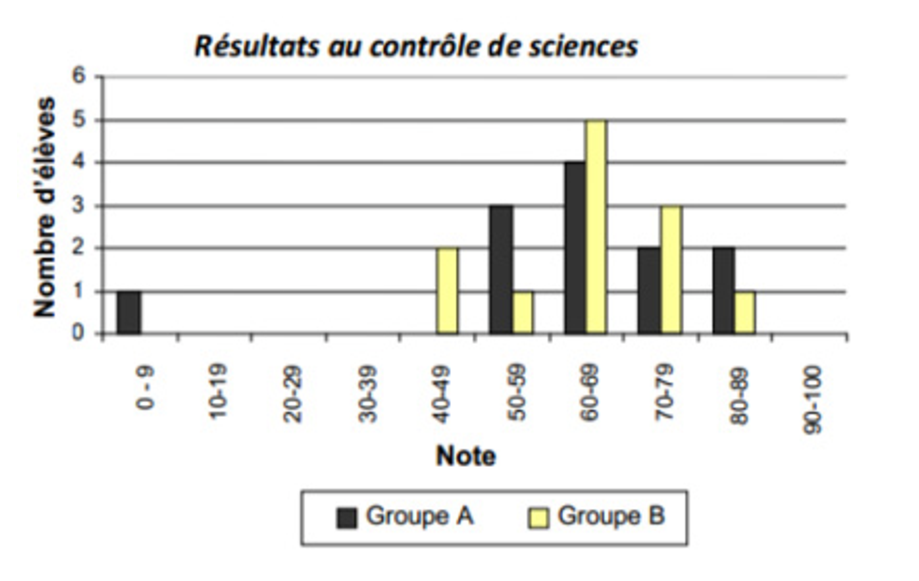
\includegraphics[scale=0.6]{Stat-13.eps} 
\end{center}
\end{minipage}
En vous servant du graphique, donnez un argument mathématique que les élèves du Groupe A pourraient utiliser. 


\end{AD}

\begin{AD}

On a représenté sur le diagramme suivant les vols du mois de février d’une compagnie aérienne.  
\begin{center}
\definecolor{xdxdff}{rgb}{0.49019607843137253,0.49019607843137253,1.}
\definecolor{ffdxqq}{rgb}{1.,0.8431372549019608,0.}
\definecolor{ffffqq}{rgb}{1.,1.,0.}
\definecolor{ffxfqq}{rgb}{1.,0.4980392156862745,0.}
\definecolor{ffqqqq}{rgb}{1.,0.,0.}
\definecolor{xfqqff}{rgb}{0.4980392156862745,0.,1.}
\definecolor{qqqqff}{rgb}{0.,0.,1.}
\begin{tikzpicture}[line cap=round,line join=round,>=triangle 45,x=1.0cm,y=1.0cm]
\clip(-0.096,-0.204) rectangle (18.304,8.336);
\draw[color=xfqqff,fill=xfqqff,fill opacity=1.0] (5.,3.5757359312880714) -- (5.424264068711929,3.5757359312880714) -- (5.424264068711929,4.) -- (5.,4.) -- cycle; 
\draw [shift={(5.,4.)},color=ffqqqq,fill=ffqqqq,fill opacity=1.0] (0,0) -- (0.:0.6) arc (0.:30.488940499830935:0.6) -- cycle;
\draw [shift={(5.,4.)},color=ffxfqq,fill=ffxfqq,fill opacity=0.95] (0,0) -- (30.488940499830935:0.6) arc (30.488940499830935:59.44286434307001:0.6) -- cycle;
\draw [shift={(5.,4.)},fill=black,fill opacity=1.0] (0,0) -- (59.44286434307001:0.6) arc (59.44286434307001:90.:0.6) -- cycle;
\draw [shift={(5.,4.)},color=qqqqff,fill=qqqqff,fill opacity=0.44]  plot[domain=1.5707963267948966:4.71238898038469,variable=\t]({1.*4.*cos(\t r)+0.*4.*sin(\t r)},{0.*4.*cos(\t r)+1.*4.*sin(\t r)});
\draw [shift={(5.,4.)},color=xfqqff,fill=xfqqff,fill opacity=0.66]  (0,0) --  plot[domain=-1.5707963267948966:0.,variable=\t]({1.*4.*cos(\t r)+0.*4.*sin(\t r)},{0.*4.*cos(\t r)+1.*4.*sin(\t r)}) -- cycle ;
\draw [shift={(5.,4.)},color=ffqqqq,fill=ffqqqq,fill opacity=0.6]  (0,0) --  plot[domain=0.:0.5321323971666955,variable=\t]({1.*4.*cos(\t r)+0.*4.*sin(\t r)},{0.*4.*cos(\t r)+1.*4.*sin(\t r)}) -- cycle ;
\draw [shift={(5.,4.)},color=ffxfqq,fill=ffxfqq,fill opacity=0.4]  (0,0) --  plot[domain=0.5321323971666955:1.037473699602908,variable=\t]({1.*3.973415659102379*cos(\t r)+0.*3.973415659102379*sin(\t r)},{0.*3.973415659102379*cos(\t r)+1.*3.973415659102379*sin(\t r)}) -- cycle ;
\draw [shift={(5.,4.)},color=ffffqq,fill=ffffqq,fill opacity=0.5]  (0,0) --  plot[domain=1.037473699602908:1.5707963267948966,variable=\t]({1.*4.*cos(\t r)+0.*4.*sin(\t r)},{0.*4.*cos(\t r)+1.*4.*sin(\t r)}) -- cycle ;
\draw (10.644,6.776) node[anchor=north west] {Vols vers l'Asie};
\draw (10.664,6.176) node[anchor=north west] {Vols vers l'Afrique};
\draw (10.664,5.616) node[anchor=north west] {Vols vers l'Amérique};
\draw (10.704,5.056) node[anchor=north west] {Vols vers l'Europe};
\draw (10.724,4.436) node[anchor=north west] {Vols vers la France};
\begin{scriptsize}
\draw [fill=ffffqq] (10.304,6.636) circle (2.5pt);
\draw [fill=ffdxqq] (10.304,6.036) circle (2.5pt);
\draw [fill=ffqqqq] (10.324,5.436) circle (2.5pt);
\draw [fill=xfqqff] (10.344,4.836) circle (2.5pt);
\draw [fill=xdxdff] (10.364,4.236) circle (2.5pt);
\end{scriptsize}
\end{tikzpicture}
\end{center}

\begin{minipage}{8cm}
Dans chaque cas, quelle fréquence représentent les vols vers la France, l’Europe et l’Asie. 
\end{minipage}
\begin{minipage}{1cm}
$~~$
\end{minipage}
\begin{minipage}{8cm}
Au mois de février, cette compagnie a affrété 576 vols. Calculer le nombre de vols vers la France, l’Europe et l’Asie. 
\end{minipage}

\end{AD}



\begin{autoeval}
\begin{tabular}{p{12cm}p{0.5cm}p{0.5cm}p{0.5cm}p{1cm}}
\textbf{Compétences visées} &  M I & MF & MF  & TBM \vcomp \\ 
Lire des données sur différents supports & $\square$ & $\square$  & $\square$ & $\square$ \vcomp \\ 
\end{tabular}
{\footnotesize MI : maitrise insuffisante ; MF = Maitrise fragile ; MS = Maitrise satisfaisante ; TBM = Très bonne maitrise}
 
\end{autoeval} % Calcul de moyenne, écart type 
%% \impress{\impressionEleve}{\include{Stat-F1_cor}}% Calcul de moyenne, de médiane 
%\begin{titre}[Arithmétique]

\Titre{Multiples, diviseurs, nombres premiers}{4}
\end{titre}

\begin{CpsCol}
\begin{description}
\item[$\square$] Modéliser et résoudre des problèmes mobilisant les notions de multiple, de diviseur,
de nombre pair, de nombre impair, de nombre premier.
\item[$\square$] Pour des entiers a et b donnés, déterminer le plus grand multiple de a inférieur ou
égal à b.
\item[$\square$] Déterminer si un entier naturel est premier.
\end{description}
\end{CpsCol}

\begin{DefT}{Diviseur}\index{Diviseur}
Soient $a$ et $b$ deux nombres relatifs. $a$ est un diviseur de $b$ lorsqu'il existe un entier $k$ tel que $b = k  \times a$. Les 3 assertions sont équivalentes :
\begin{description}
\item[•] $b$ est un multiple de $a$.
\item[•] $a$ est un diviseur de $b$.
\item[•] $b$ est un divisible par $a$.
\end{description}
\end{DefT}

\begin{Ex}
3 est un diviseur de 36. En effet, $36 = 3 \times 12$ et $12 \in \Z$.
\end{Ex}

\EPC{1}{FEA-17}{Raisonner. Calculer. } 

\begin{DefT}{Fraction irréductible}\index{Fraction irréductible}
Une fraction est irréductible lorsqu'il n'est pas possible de la simplifier, autrement dit lorsque le numérateur et le dénominateur n'ont pas de diviseur commun.
\end{DefT}

\begin{ROC}

Démontrer que $\frac{1}{3}$ n'est pas décimal.
\end{ROC}





\begin{DefT}{Nombre pair et impair}\index{Nombre pair et impair}
Soit $a$ un entier. 
\begin{description}
\item[•] $a$ est pair lorsqu'il existe un entier $n$ tel que $a = 2\times n$.
\item[•]  $a$ est impair lorsqu'il existe un entier $n$ tel que $a = 2\times n +1$.
\end{description}
\end{DefT}


\begin{Th}
 
Soit $a$ un entier ($a \in \Z)$. $a^2$ est impair si et seulement si $a$ est impair.
\end{Th}

\EPCN{Raisonner. }

Démontrer ce résultat.

\begin{Th} 

Soit $a$ un entier ($a \in \Z)$. Si $b$ et $b'$ sont deux multiples de $a$ alors $b+b'$ est un multiple de $a$.
\end{Th}

\EPCN{Raisonner. }

Démontrer ce résultat.



\begin{DefT}{Nombre premier}
Un entier naturel est dit nombre premier lorsqu'il possède exactement deux diviseurs : 1 et lui-même.
\end{DefT}


\begin{Rq} 
Un nombre premier est supérieur ou égal à 2. 1 n'est pas premier, il ne possède qu'un seul diviseur.
\end{Rq}


\mini{
\EPCN{Raisonner.}

Soit $a$ un entier impair. Démontrer que $a^3$ est un nombre impair.


\EPCN{Raisonner.}

Une crèche dispose de 60 dalles carrées en mousse. Elle souhaite les placer de manière à former un rectangle.

\begin{enumerate}
\item Quelles sont les dimensions possibles de ce rectangle ?
\item Quel est celui qui le plus grand périmètre ?
\end{enumerate}


\EPCN{Chercher.}

La conjecture de Goldbach affirme que "tout nombre pair supérieur ou égal à 4 est la somme de deux nombres premiers".

\begin{enumerate}
\item Vérifier cette conjecture pour tout nombre pairs de l'intervalle [10;20].
\item Trouver tous les nombres premiers $p$ et $p'$ tels que $p+p'=100$.
\item Déterminer une algorithme pour déterminer $p$ et $p'$.
\end{enumerate}


\EPCP{1}{FEA-102}{Modéliser. Calculer.}

\begin{ROC}

On cherche à démontrer que $\sqrt2$ n'est pas rationnel.
On raisonne par l'absurde. On suppose $\sqrt{2}$ s'écrit sous forme d'une fraction irréductible $\frac{a}{b}$, $a$ et $b$ deux entiers naturels non nuls.

\begin{enumerate}
\item Démontrer que $2b^2=a^2$.
\item En déduire que $a^2$ est pair donc $a$ est pair.
\item Démontrer alors que $b^2$ est pair. Conclure.
\end{enumerate}



\end{ROC}




}{

\EPCN{Chercher.}

On considère un nombre premier $p \geq 6$. 
\begin{enumerate}
\item Démontrer que $p=6q+1$ ou $p=6q+5$, avec $q$ un entier naturel non nul.
\item On suppose que $p=6q+1$.
  \begin{enumerate}
  \item Justifier que $p^2=12q(3q+1)+1$. 
  \item Quelle est la parité de $q(3q+1)$ ?
  \item En déduire qu'il existe un entier naturel $k$ tel que $p^2 = 24k +1$.
  \end{enumerate}
\item On suppose que $p=6q+5$. Démontrer qu'il existe un entier naturel $k$ tel que $p^2 = 24k +1$.
 \end{enumerate}

\EPCN{Chercher.}

On considère un entier naturel $n$.
  \begin{enumerate}
  \item Démontrer que $n^2+n$ est pair. 
  \item Démontrer que le chiffre des unités de $n^2+n$ n'est jamais égal à 4 ou 8.
  \end{enumerate}
 
\EPCP{1}{FEA-101}{Modéliser. Calculer.}
}



 % Multiples et diviseur
% \begin{titreTice}[Synthèse]

\Titre{Nombres et calculs}{2}
\end{titreTice}


\EPCN{Calculer.}

Soient $x$ et $y$ deux réels tels que $x=\frac{y-3}{8-2y}$.

\begin{enumerate}
\item Pour quelles valeurs de $y$ cette égalité est-elle définie ?
\item Exprimer $y$ en fonction de $x$. Préciser les valeurs de $x$ pour lesquelles cette égalité $y=f(x)$ est définie.
\end{enumerate}


\EPCN{Représenter. Calculer.}

Dans un repère du plan, $d$ et $d'$ sont deux droites d'équations respectives $2x-3y+5=0$ et $5y+4x-1=0$. Déterminer les coordonnées du point d'intersection de $d$ et de $d'$. 


\EPCN{Représenter. Calculer.}

$x$ et $y$ sont deux réels non nuls. Comparer les nombres $A = \frac{-2xy}{x-y}$ et $B=\frac{x-y}{2}$.


\EPCN{Représenter. Calculer.}

\begin{enumerate}
\item Donner l'ensemble des diviseurs positifs de 36.
\item En déduire les solutions de $x(x+5)=36$.
\end{enumerate}

\EPCN{Représenter. Calculer.}

Soit $N$ un entier naturel, impair et non premier. On suppose que $N=a^2-b^2$ où $a$ et $b$ sont deux entiers naturels.

\begin{enumerate}
\item Montrer que $a$ et $b$ n'ont pas la même parité.
\item Montrer que $N$ peut s'écrire comme produit de deux entiers naturels $p$ et $q$.
\item Quelle est la parité de $p$ et $q$ ? 
\end{enumerate}


\EPCN{Représenter. Calculer.}

On considère un entier naturel $n$ non nul. 

\begin{enumerate}
\item On suppose $S_n = 1+2+3+...+(n-2)+(n-1)+n$ 
\begin{enumerate}
\item En remarquant que $S_n = n + (n-1)+ (n-2)+ ...+3+2+1$, déterminer une expression de $2S_n$ en fonction de $n$.
\item En déduire une expression de $S_n$ en fonction de $n$.
\item Calculer $1+2+3+...+1031$.
\end{enumerate}
 \item En déduire des questions précédentes que $n(n+1)$ est un nombre pair pour tout entier entier naturel $n$ non nul.
\end{enumerate}


 %  Nombres et calculs
%\begin{titre}[Géométrie vectorielle et analytique]

\Titre{Projection orthogonale}{3}
\end{titre}

\begin{CpsCol}
\textbf{Démontrer avec les vecteurs}
\begin{description}
\item[$\square$] Résoudre des problèmes de géométrie plane sur des figures simples ou complexes
(triangles, quadrilatères, cercles).
\item[$\square$] Calculer des longueurs, des angles, des aires et des volumes.
\item[$\square$] Traiter de problèmes d’optimisation. 
\end{description}
\end{CpsCol}



\begin{DefT}{Projection orthogonale}\index{Projection orthogonale}
Soit $d$ une droite du plan et $A$ un point extérieur à $d$. La projection orthogonale est l'application du plan qui  au point $A$ associe le point $A'$ de la droite $d$ tel que la droite $(AA')$ est perpendiculaire à $d$ en $A'$. 

\definecolor{xdxdff}{rgb}{0.49019607843137253,0.49019607843137253,1.}
\definecolor{ududff}{rgb}{0.30196078431372547,0.30196078431372547,1.}
\begin{tikzpicture}[line cap=round,line join=round,>=triangle 45,x=0.5cm,y=0.5cm]
\clip(0.831296100794201,-0.7348563902439222) rectangle (17.486323662311374,5.80145736585363);
\draw[line width=2.pt,fill=black,fill opacity=0.10000000149011612] (9.190921775722733,1.1160512934995357) -- (9.06194825746555,1.7700717388119918) -- (8.407927812153094,1.6410982205548086) -- (8.536901330410277,0.9870777752423525) -- cycle; 
\draw [line width=2.pt,domain=0.831296100794201:17.486323662311374] plot(\x,{(-17.201085830991378--4.87081073170731*\x)/24.699720119533016});
\draw [line width=2.pt,dash pattern=on 3pt off 3pt,domain=0.831296100794201:17.486323662311374] plot(\x,{(-215.6669425698831--24.699720119533016*\x)/-4.87081073170731});
\draw (2.119703893288926,1.0563449756097338) node[anchor=north west] {$d$};
\begin{scriptsize}
\draw [fill=ududff] (-5.453619960155669,-1.7718677073170916) circle (2.5pt);
\draw[color=ududff] (-5.155086447260557,-1.1119514146341656) node {$A_1$};
\draw [fill=ududff] (19.246100159377345,3.098943024390219) circle (2.5pt);
\draw[color=ududff] (19.466072221510586,3.6802978536585105) node {$B$};
\draw[color=black] (-13.43546335756202,-2.793166731707334) node {$f$};
\draw [color=xdxdff] (8.536901330410277,0.9870777752423525)-- ++(-2.5pt,0 pt) -- ++(5.0pt,0 pt) ++(-2.5pt,-2.5pt) -- ++(0 pt,5.0pt);
\draw[color=xdxdff] (8.02752499058181,0.5378393170731492) node {$A'$};
\draw[color=black] (6.267748493515845,10.405159121951185) node {$g$};
\draw [color=xdxdff] (7.748641917797854,4.984315185099545)-- ++(-2.5pt,0 pt) -- ++(5.0pt,0 pt) ++(-2.5pt,-2.5pt) -- ++(0 pt,5.0pt);
\draw[color=xdxdff] (7.964675829972312,5.565772975609728) node {$A$};
\end{scriptsize}
\end{tikzpicture}


\end{DefT}



\begin{Rq}
Tout point du plan a un unique projeté orthogonal sur une droite $d$.

Tout point $M$ de la droite $d$ est le projeté orthogonal d'une infinité de point du plan qui appartiennent à la droite passant par $M$ et perpendiculaire à $M$.

\definecolor{xdxdff}{rgb}{0.49019607843137253,0.49019607843137253,1.}
\definecolor{ududff}{rgb}{0.30196078431372547,0.30196078431372547,1.}
\begin{tikzpicture}[line cap=round,line join=round,>=triangle 45,x=0.5cm,y=0.5cm]
\clip(2.2454022145079233,-3.468795317073187) rectangle (14.406714792445936,7.749781658536554);
\draw[line width=2.pt,fill=black,fill opacity=0.10000000149011612] (9.190921775722733,1.1160512934995357) -- (9.06194825746555,1.7700717388119918) -- (8.407927812153094,1.6410982205548086) -- (8.536901330410277,0.9870777752423525) -- cycle; 
\draw [line width=2.pt,domain=2.2454022145079233:14.406714792445936] plot(\x,{(-17.201085830991378--4.87081073170731*\x)/24.699720119533016});
\draw [line width=2.pt,dash pattern=on 6pt off 6pt,domain=2.2454022145079233:14.406714792445936] plot(\x,{(-215.6669425698831--24.699720119533016*\x)/-4.87081073170731});
\draw (2.119703893288926,1.0563449756097338) node[anchor=north west] {$d$};
\begin{scriptsize}
\draw [fill=ududff] (-5.453619960155669,-1.7718677073170916) circle (2.5pt);
\draw[color=ududff] (-5.155086447260557,-1.1119514146341656) node {$A_1$};
\draw [fill=ududff] (19.246100159377345,3.098943024390219) circle (2.5pt);
\draw[color=ududff] (19.466072221510586,3.6802978536585105) node {$B$};
\draw[color=black] (-13.43546335756202,-2.793166731707334) node {$f$};
\draw [color=xdxdff] (8.536901330410277,0.9870777752423525)-- ++(-2.5pt,0 pt) -- ++(5.0pt,0 pt) ++(-2.5pt,-2.5pt) -- ++(0 pt,5.0pt);
\draw[color=xdxdff] (7.9332512496675625,0.5378393170731492) node {$M$};
\draw[color=black] (6.267748493515845,10.405159121951185) node {$g$};
\draw [color=xdxdff] (7.748641917797854,4.984315185099545)-- ++(-2.5pt,0 pt) -- ++(5.0pt,0 pt) ++(-2.5pt,-2.5pt) -- ++(0 pt,5.0pt);
\draw[color=xdxdff] (7.964675829972312,5.565772975609728) node {$A$};
\draw [color=xdxdff] (9.048175607643872,-1.6055771743290161)-- ++(-2.5pt,0 pt) -- ++(5.0pt,0 pt) ++(-2.5pt,-2.5pt) -- ++(0 pt,5.0pt);
\draw[color=xdxdff] (9.253083622467036,-1.0333899512195315) node {$C$};
\draw [color=xdxdff] (9.229394525056087,-2.524532310751975)-- ++(-2.5pt,0 pt) -- ++(5.0pt,0 pt) ++(-2.5pt,-2.5pt) -- ++(0 pt,5.0pt);
\draw[color=xdxdff] (9.441631104295533,-1.9447029268292864) node {$D$};
\draw [color=xdxdff] (7.474252237411067,6.375736178964803)-- ++(-2.5pt,0 pt) -- ++(5.0pt,0 pt) ++(-2.5pt,-2.5pt) -- ++(0 pt,5.0pt);
\draw[color=xdxdff] (7.6818546072295675,6.948454731707288) node {$E$};
\end{scriptsize}
\end{tikzpicture}

\end{Rq}

\EPCG{1}{GVA-63}{Représenter. Calculer.}


\EPCG{1}{GVA-64}{Raisonner. Représenter. Calculer.}


\EPCG{1}{GVA-59}{Représenter. Calculer.}



\EPCG{1}{GVA-59}{Représenter}

 

\EPCG{1}{GVA-60}{Représenter}

\App{1}{GVA-13}
 

\EPCG{1}{GVA-61}{Modéliser. Représenter. Calculer.}


\begin{ROC}

Le projeté orthogonal du point M sur une droite $\Delta$ est le point de la droite $\Delta$ le plus
proche du point M.
\end{ROC}


\begin{Approfondissement}

\begin{enumerate}
\item Démontrer que les trois médiatrices d'un triangle quelconque ABC sont concourantes.
\item Démontrer que les trois hauteurs d'un triangle quelconque ABC sont concourantes.
\end{enumerate}

\end{Approfondissement}


  % Projection orthogonale.
%\include{Stat-F1_bis} % Calcul de médiane, de quartiles 
%% \begin{titre}[Les statistiques]

{\color{bleu3}{\LARGE Calcul de moyenne} \hfill{Niveau 2}}
\end{titre}



\begin{CpsCol}
\textbf{Interpréter, représenter et traiter des données}
\begin{description}
\item[$\square$] Calculer une moyenne
\item[$\square$] Interpréter une caractéristique de position
\end{description}
\end{CpsCol}

\begin{Rec}

Si 2/5 des habitants d'un pays ont au moins 50 ans et 1/3 des habitants de ce pays ont moins de 20 ans, est-il possible que l'âge moyen de la population soit de 40 ans ?

\hfill{D’après le cadre d’évaluation «PISA 2006»:}
 
\hfill{items libérés Mathématiques OCDE/DEPP – janvier 2011}


\end{Rec}

\begin{DefT}{moyenne}
La \textbf{moyenne} d'une série statistique est le quotient de la somme de TOUTES les valeurs par l'effectif total de cette série.
\end{DefT}

\begin{Ex}
Voici les notes obtenues par Aurélie en Mathématiques au cours de l'année. 
\begin{itemize}
\item	1er trimestre :		10 – 9 – 11 – 12 – 11,5 – 14 – 12
\item	2ème trimestre :	9,5 – 11 – 12,5 – 8 – 13 – 18
\item	3ème trimestre :	8 – 9 – 14 – 12 – 10 – 13 – 11,5
\end{itemize}
Calculons sa moyenne annuelle :
		$m1 =\frac{10+9+11+\ldots{}+11,5}{20}=\frac{229}{20}=11,45$ 
\end{Ex}
		

\begin{AD}

\begin{multicols}{2}
Voici ci-contre la répartition par âge des membres d'un club d'échec.
Quel est l'age moyen des adhérents ?

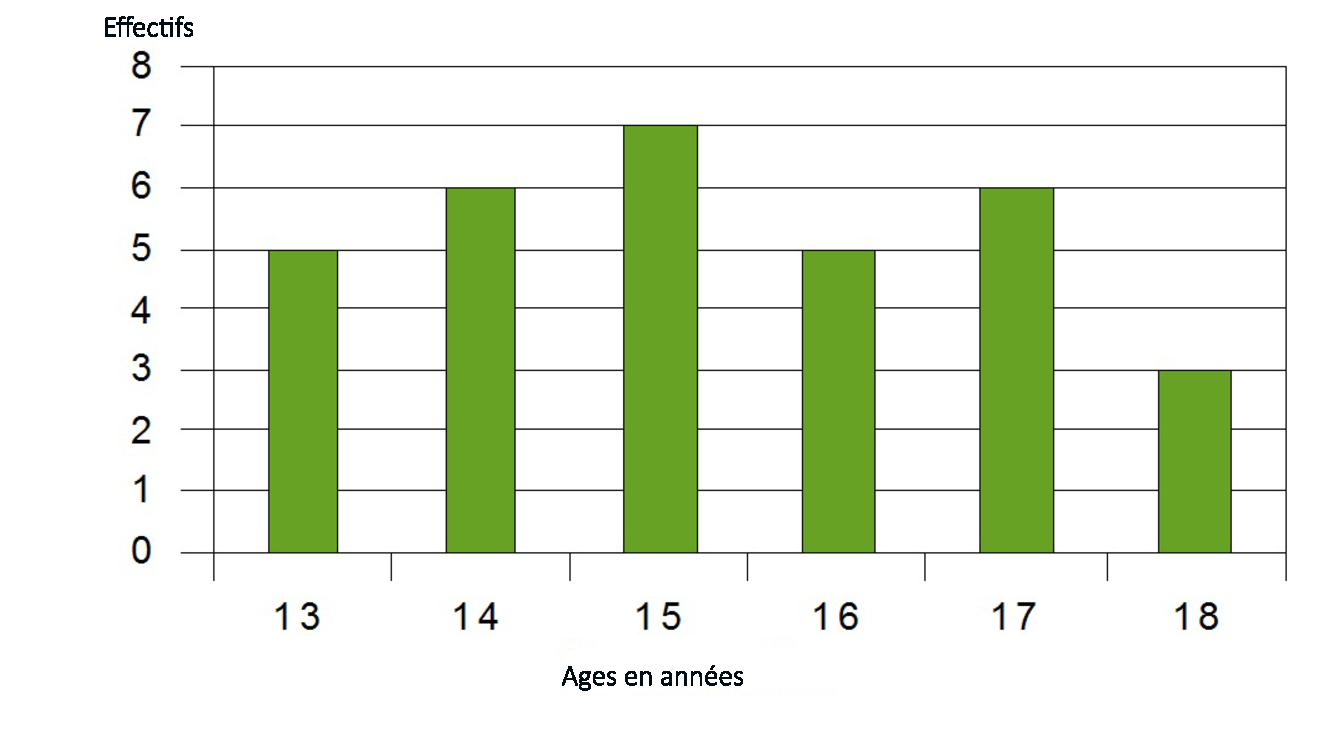
\includegraphics[scale=0.35]{Stat-cours1.eps} 
\end{multicols}	
\end{AD}


 


\begin{tabular}{|c|c|c|c|c|c|}
\hline 
heures & $0\leq h < 4$ & $4 \leq h < 8$ & $8 \leq h < 12$ & $12 \leq h < 16$ & $16 \leq h$ \\ 
\hline 
températures & 12 & 18 & 22 & 30 & 26 \\ 
\hline 
\end{tabular} 



\subsection*{Moyenne de moyennes}
\begin{Ex}
		
Avec l'exemple précédent :
\begin{itemize}
\item 		1er trimestre :	  la moyenne d'Aurélie est $11,36$ ;
\item		2ème trimestre : la moyenne d'Aurélie est $12$ ;
\item		3ème trimestre : la moyenne d'Aurélie est $11,07$.
\end{itemize}
Calculons la moyenne de ses moyennes trimestrielles :
		$m2 =\frac{11,36+12+11,07}{3}=\frac{34,43}{3}$ donc  		$m2\approx 11,48$
\end{Ex}
				
		
		
\begin{Rq}	
Cette moyenne est rarement égale à la moyenne de la série.

La moyenne est toujours comprise entre la plus petite valeur et la plus grande valeur de la série statistique.
\end{Rq}



\begin{AD}

Voici les notes d'un élève de 4\ieme\ en mathématiques.
\medskip
\begin{description}
 \item [1\ier\ trimestre] 15\kern5mm 10\kern5mm 8\kern5mm 13\kern5mm 10
\item[2\ieme\ trimestre] 13\kern5mm 9\kern5mm 7\kern5mm 14\kern5mm 13\kern5mm 16
\item[3\ieme\ trimestre] 12\kern5mm 15\kern5mm 17\kern5mm 14\kern5mm 12
\end{description}
\begin{enumerate}
  \item Calcule sa moyenne pour chacun des trois trimestres.
  \item Calcule la moyenne des moyennes des trois trimestres.
  \item Calcule la moyenne de l'ensemble de ses notes sur son année de 4\ieme.\\Que remarque-t-on ?
\end{enumerate}
\end{AD}

\begin{AD}

On a trié 4 paquets de 40 M\&M's et on a obtenu les résultats suivants : 


\begin{center}
 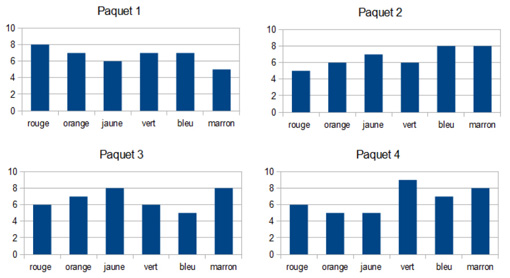
\includegraphics[scale=0.5]{mms1.jpg}
 \end{center} 


\begin{enumerate}
\item Calcule le nombre de bonbons bleus dans ces 4 paquets.
\item Combien en moyenne a-t-on de M\&M's bleus par paquets ? 
\end{enumerate}


\end{AD}

\begin{Exo}

\begin{minipage}[top]{10cm}
L'entreprise est à la recherche de qualifications de plus en plus élevées pour faire face au développement de technologies en constante évolution et pour une bonne compréhension des consignes de travail. Lors de sa scolarité, un jeune doit développer de l'intérêt et de la curiosité, si utiles pour réussir ensuite sa vie professionnelle. Face au nombre, en baisse mais encore inquiétant, de sorties du système scolaire sans qualification, il paraît intéressant d'étudier ce phénomène du point de vue européen à la lumière des mathématiques. En France, 13\% des jeunes de 18 à 24 ans qui ne poursuivent pas d'études ni de formation n'ont ni CAP, ni BEP, ni bac et sont sortants précoces.
\end{minipage}
\begin{minipage}{6cm}
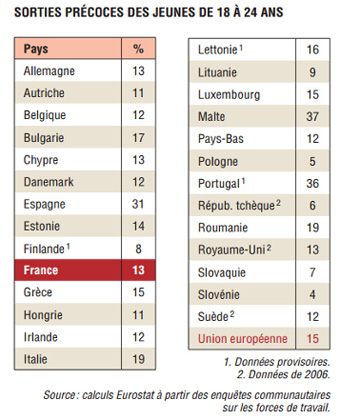
\includegraphics[scale=0.5]{stat12.jpg} 
\end{minipage}

\begin{enumerate}
\item Calculer la moyenne des sorties précoces en Europe à l'aide des données du tableau. Que remarquez-vous ? Justifier.
\item Tracer une représentation graphique de ce tableau sur tableur ou sur une feuille.
\item Compléter le tableau suivant et construire l'histogramme de cette série.

\begin{tabular}{|c|c|c|c|c|c|c|}
\hline 
Sorties précoces en 2007 & [0;5[ & [5;10[ & [10;15[ & [15;20[ & [20;25[ & [25;30] \\ 
\hline 
Nombre de pays européens &  &  &  &  &  &  \\ 
\hline 
\end{tabular} 

\item Calculer la moyenne des sorties précoces en Europe à l'aide de la question 3. Comparer le résultat avec la question 1.  
\end{enumerate}




  
\end{Exo}



\begin{DefT}{moyenne pondérée}
La \textbf{moyenne pondérée} d’une série statistique est le quotient de la somme
de TOUTES les valeurs multipliées chacune par leur coefficients
par la somme de ces coefficients.
\end{DefT}

\begin{AD}

Pierre, Jean et Alain ont passé un examen comportant quatre
disciplines. Pour être reçu, il faut atteindre 10 de moyenne.
\begin{enumerate}
\item Calculer la moyenne, sans coefficient, des trois candidats.
\begin{center}
  \begin{tabular}{|c|c|c|c|c|}
\cline{2-5}
\multicolumn{1}{c|}{}&Français&Mathématiques&Anglais&Technologie\\
\hline
Pierre&15&9&11&7\\
\hline
Jean&10&11&12&9\\
\hline
Alain&7&14&13&8\\
\hline
  \end{tabular}
\end{center}
\item Pour cet examen, le français, les mathématiques, l'anglais et la
technologie ont respectivement pour coefficient 6; 4; 2 et 5.\par
Calculer la moyenne pondérée de chaque candidat et dire s'ils sont reçus
ou non.
\end{enumerate}
\end{AD}

\begin{AD}

Lors d'un test d'endurance, plusieurs élèves ont eu 12 minutes pour
parcourir la plus grande distance possible. Voici les résultats des
élèves :
2230 -- 2450 -- 1890 -- 1850 -- 2650 -- 2630 -- 2110 -- 2250 -- 2180 --
1980 -- 2000 -- 2850 -- 1950 -- 2920 -- 1975 -- 1910 -- 1860 -- 1930 --
2010 -- 2400 -- 2650 -- 2320 -- 2190 -- 2730 -- 2120 -- 2380 -- 2220.

\begin{enumerate}
\item
Calcule la moyenne des distances parcourues.

\item
On veut calculer la moyenne approximative des distances parcourues.
Pour cela, dénombrer le nombre d'élèves dans chacun des intervalles
suivants :\\
\hskip 0pt plus 500pt minus 500pt\begin{tabular}{|*{6}{c|}}
\hline
$[1800 ; 2000 [$ & $[2000 ; 2200 [$ &
$[2200 ; 2400 [$ & $[2400 ; 2600 [$ &
$[2600 ; 2800 [$ & $[2800 ; 3000 [$ \\
\hline
&&
 &&& \\
\hline
\end{tabular}\hskip 0pt plus 500 pt minus 500 pt\strut
\item
Calculer une moyenne approchée en remplaçant la distance de chaque élève
	par le début de chaque intervalle (1800 pour le premier, 2000 pour
	le deuxième,\dots) en pensant à remplacer chaque série de nombres
	identiques par une multiplication.
	
\item Reprendre la question précédente en 
	remplaçant la distance de chaque élève
	par le milieu de chaque intervalle (1900 pour le premier, 2100 pour
	le deuxième,\dots)
	
\item Reprendre la question précédente en 
	remplaçant la distance de chaque élève
	par la fin de chaque intervalle (2000 pour le premier, 2200 pour
	le deuxième,\dots)
	
\end{enumerate}
\end{AD}

\begin{AD}

Le professeur d'EPS a relevé les performances ci-dessous :
\begin{center}
  \begin{tabularx}{0.85\linewidth}{|l|X|X|l|X|X|}
    \hline
\multicolumn{1}{|c|}{Noms}&Temps au 80~m (s)&Hauteur du saut (cm)&\multicolumn{1}{c|}{Noms}&Temps au 80~m (s)&Hauteur du saut (cm)\\
\hline
Charles&\multicolumn{1}{c|}{13}&\multicolumn{1}{c|}{110}&Gérald&\multicolumn{1}{c|}{13,6}&\multicolumn{1}{c|}{115}\\
Bruno&\multicolumn{1}{c|}{12,5}&\multicolumn{1}{c|}{120}&Nicolas&\multicolumn{1}{c|}{13,9}&\multicolumn{1}{c|}{110}\\
Sylvie&\multicolumn{1}{c|}{15}&\multicolumn{1}{c|}{100}&Florence&\multicolumn{1}{c|}{14,7}&\multicolumn{1}{c|}{110}\\
Brice&\multicolumn{1}{c|}{13,2}&\multicolumn{1}{c|}{125}&Daniel&\multicolumn{1}{c|}{13}&\multicolumn{1}{c|}{125}\\
Carine&\multicolumn{1}{c|}{15,4}&\multicolumn{1}{c|}{100}&Viviane&\multicolumn{1}{c|}{16}&\multicolumn{1}{c|}{95}\\
Léon&\multicolumn{1}{c|}{12}&\multicolumn{1}{c|}{135}&Barbara&\multicolumn{1}{c|}{15,1}&\multicolumn{1}{c|}{105}\\
Christian&\multicolumn{1}{c|}{12,6}&\multicolumn{1}{c|}{130}&Jeanne&\multicolumn{1}{c|}{14,9}&\multicolumn{1}{c|}{110}\\
\'Elisabeth&\multicolumn{1}{c|}{15,4}&\multicolumn{1}{c|}{95}&Lucie&\multicolumn{1}{c|}{15,4}&\multicolumn{1}{c|}{100}\\
Aude&\multicolumn{1}{c|}{14,9}&\multicolumn{1}{c|}{110}&Odile&\multicolumn{1}{c|}{14,2}&\multicolumn{1}{c|}{85}\\
Cécile&\multicolumn{1}{c|}{16,2}&\multicolumn{1}{c|}{85}&Alice&\multicolumn{1}{c|}{15,6}&\multicolumn{1}{c|}{105}\\
Clément&\multicolumn{1}{c|}{12}&\multicolumn{1}{c|}{140}&Gaël&\multicolumn{1}{c|}{13,5}&\multicolumn{1}{c|}{125}\\
Cathy&\multicolumn{1}{c|}{15,8}&\multicolumn{1}{c|}{100}&Pierre&\multicolumn{1}{c|}{12,3}&\multicolumn{1}{c|}{135}\\
Delphine&\multicolumn{1}{c|}{15}&\multicolumn{1}{c|}{105}&Armand&\multicolumn{1}{c|}{12,8}&\multicolumn{1}{c|}{130}\\
Jacques&\multicolumn{1}{c|}{13,1}&\multicolumn{1}{c|}{135}&Jean&\multicolumn{1}{c|}{13,1}&\multicolumn{1}{c|}{115}\\
André&\multicolumn{1}{c|}{13,9}&\multicolumn{1}{c|}{120}&David&\multicolumn{1}{c|}{12,5}&\multicolumn{1}{c|}{135}\\
\hline
  \end{tabularx}
\end{center}
\begin{enumerate}
  \item
    \begin{enumerate}
    \item Quel est le temps moyen mis pour effectuer le 80~m ?
    \item Combien d'élèves ont un temps supérieur au temps moyen ?
    \end{enumerate}
  \item
    \begin{enumerate}
    \item Quelle est la hauteur moyenne d'un saut ?
    \item Combien d'élèves ont une hauteur inférieure à la hauteur
      moyenne ?
    \end{enumerate}
\end{enumerate}

\end{AD}

\subsection*{Utilisation d'un tableur pour le calcul de la moyenne}

Le tableur est un outil performant pour calculer la moyenne.


\begin{Ex}
Sur la feuille de classeur ci-dessous,
on a calculé la longueur moyenne des prénoms des 684 élèves du collège.\\
		Les longueurs des prénoms sont rangées de la cellule C4 à la cellule C687.\\
		Ces cellules se suivent, on dit qu'elles sont contiguës.\\
		Dans la formule, on utilise alors le symbole \og  deux – points \fg{}.\\
		Dans la zone de saisie des fonctions, on a tapé : =MOYENNE(C4:C687).\\
		
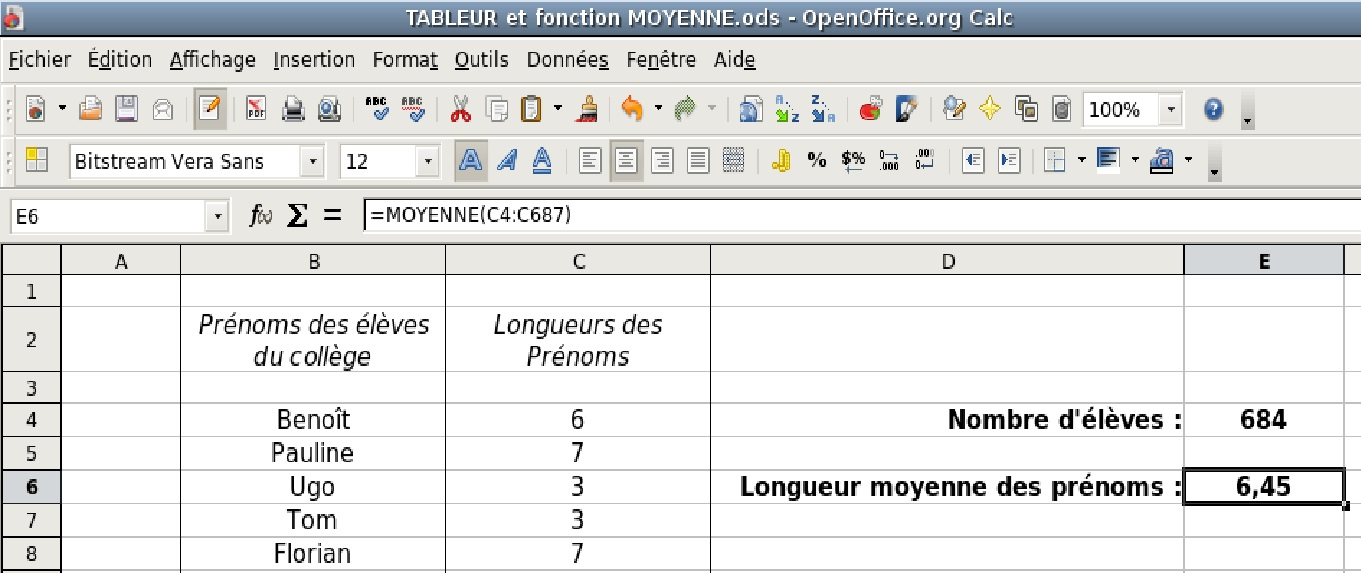
\includegraphics[scale=0.5]{Stat-cours2.jpg} 		
\end{Ex}

\begin{AD}

Lors de la première édition de la Course aux Nombres, les 24 élèves de la classe de Cinquième 2 en Colombie ont obtenu les résultats suivants. Les notes sont évaluées sur 30 points.


\begin{enumerate}
\item Reproduire la feuille de calcul comme indiqué ci dessous.

\begin{tabular}{|c|c|c|c|c|c|c|c|c|c|}
\hline 
\rowcolor{gray} & A & B & C & D & E & F & G & H & I \\ 
\hline 
\cellcolor{gray} 1 & 11 & 16 & 22 & 20 & 26 &  &  & Nombres d'élèves total &  \\ 
\hline 
\cellcolor{gray}2& 26 & 18 & 26 & 19& 16 &  &  & Nombre d'élèves dont la nombre est égale à 22 &  \\ 
\hline 
\cellcolor{gray}3 & 17 &27 & 18 & 16 & 22 &  & & Fréquence d'élèves dont la note est égale à 22 &  \\ 
\hline 
\cellcolor{gray}4 & 16 & 19 & 11 & 21 & 17 & &  & Nombre d'élèves dont la note est égale à 19 &  \\ 
\hline 
\cellcolor{gray}5 & 22 & 15 & 22 & 23 &  &  &  & Fréquence d'élèves dont la note est égale à 19 &  \\ 
\hline 
\end{tabular} 

\item  
\begin{enumerate}
\item  Déterminer dans la cellule I1 le nombre d'élèves participants à ce jeu. 
Rappel : Pour déterminer le nombre de cases remplies d'un tableau, on utilise la syntaxe : =NB(A1:E5). 
\item  Déterminer dans la cellule I2 le nombre d'élèves dont la note est égale à 22 ? 
Rappel : Pour déterminer le nombre de cases remplies avec la valeur 22, on utilise la syntaxe : =NB.SI(A1:E5;22). 
\item  Calcule dans la cellule I3 la fréquence des élèves ayant obtenu 22.
\end{enumerate}
\item  
\begin{enumerate}
\item Détermine la moyenne de cette classe. On pourra utiliser la syntaxe "=MOYENNE(A1:E5)".
\item Explique par une phrase le calcul du tableur pour donner la moyenne.
\item 
\begin{enumerate}
\item Complète le tableau ci-dessous.

\begin{tabular}{|c|c|c|c|c|c|c|}
\hline 
Notes & $[0;5[$ &  $[5;10[$  &  $[10;15[$  &  $[15;20[$  &  $[20;25[$  &  $[25;30]$  \\ 
\hline 
Fréquence &  &  &  &  &  &  \\ 
\hline 
\end{tabular} 

\item Calcule la moyenne avec ce regroupement.	
\end{enumerate}
\item Création d'un diagramme avec un tableur
\begin{enumerate}
\item  Sélectionne la plage de données A1:E5 puis clique sur l'icône graphique
\item  Quel est le problème de la plage de données A1:E5 ?
\end{enumerate}

\end{enumerate}
\end{enumerate}




\end{AD}



\begin{AD}

\begin{enumerate}
\item Explique le fonctionnement de cet algorithme :

\begin{tabular}{|p{10cm}|}
\hline 
\#1. Somme = 0 \\ 
\#2. Moyenne = 0\\ 
\#3. Répéter 4 fois\\ 
\#4. \hspace{1cm} Demander\_une\_valeur x et attendre\\ 
\#5. \hspace{1cm} Lire réponse\\ 
\#6. \hspace{1cm} Somme prend\_la\_valeur Somme +  réponse\\ 
\#7. Moyenne = Somme / 4\\ 
\#8. Afficher Moyenne\\ 
\hline 
\end{tabular} 

\item A l'aide du logiciel Scratch, traduis cet algorithme en programme. 

\end{enumerate}

\end{AD}


\begin{autotest}
\begin{enumerate}
\item On donne les nombres suivants : $$4~~ - ~~ 16 ~~  - ~~ 8 ~~ - ~~ 13 ~~ - ~~ 15 $$
La moyenne est $$a. 11~~ ~~ ~~ b. 11,5 ~~  ~~ ~~ c. 11,2 ~~ ~~ ~~ d. 12$$

\item Pour calculer la moyenne des cellules A5 à B5, avec un tableur, on tape la formule
$$a. MOYENNE(A5:B5)~~ ~~ ~~ b. =MOYENNE(A5:B5) ~~  ~~ ~~ c. MOYENNE(A5;B5) ~~ ~~ ~~ d. =MOYENNE(A5;B5)$$

\item Voici le diagramme à bâtons des notes d'un devoir. 

\definecolor{qqqqff}{rgb}{0.,0.,1.}
\definecolor{cqcqcq}{rgb}{0.7529411764705882,0.7529411764705882,0.7529411764705882}
\begin{tikzpicture}[line cap=round,line join=round,>=triangle 45,x=1.0cm,y=1.0cm]
\draw [color=cqcqcq,, xstep=1.0cm,ystep=1.0cm] (-0.72,-1.1) grid (10.62,7.46);
\draw[->,color=black] (-0.72,0.) -- (10.62,0.);
\foreach \x in {,1.,2.,3.,4.,5.,6.,7.,8.,9.,10.}
\draw[shift={(\x,0)},color=black] (0pt,2pt) -- (0pt,-2pt) node[below] {\footnotesize $\x$};
\draw[->,color=black] (0.,-1.1) -- (0.,7.46);
\foreach \y in {-1.,1.,2.,3.,4.,5.,6.,7.}
\draw[shift={(0,\y)},color=black] (2pt,0pt) -- (-2pt,0pt) node[left] {\footnotesize $\y$};
\draw[color=black] (0pt,-10pt) node[right] {\footnotesize $0$};
\clip(-0.72,-1.1) rectangle (10.62,7.46);
\draw [color=qqqqff] (1.,0.)-- (1.,1.);
\draw [color=qqqqff] (3.,0.)-- (3.,2.);
\draw [color=qqqqff] (4.,0.)-- (4.,3.);
\draw [color=qqqqff] (5.,4.)-- (5.02,-0.14);
\draw [color=qqqqff] (6.,0.)-- (6.,6.);
\draw [color=qqqqff] (7.,6.)-- (7.,0.);
\draw [color=qqqqff] (8.,4.)-- (8.,0.);
\draw [color=qqqqff] (10.,1.)-- (10.,0.);
\draw (9.44,-0.5) node[anchor=north west] {notes};
\draw (0.16,6.42) node[anchor=north west] {Effectifs};
\end{tikzpicture}

La moyenne est $$a. \approx 5,9 ~~ ~~ ~~ b. \approx 6,5 ~~  ~~ ~~ c. \approx 1,7 ~~ ~~ ~~ d. \approx 5,5$$

\item Pierre n'a retrouvé que 7 contrôles où il a obtenu chaque fois 8 sur 10. Il a perdu une copie mais il sait que sa moyenne est de 7,75. Quelle est la note de la copie perdue ?

\item Grégory espère obtenir au Bac 17/20 en Maths, 14/20 en Lettres et 17/20 en Langues. Le coefficient de l'épreuve des maths est 7, celui de l'épreuve des lettres est 3 et celui de l'épreuve des langues est 2. Peut il espérer obtenir la mention "Très bien" ?

\item Le tableau donne le nombre de voitures qui passent dans un virage dangereux où la vitesse est limitée à 60 km/h. 

\begin{tabular}{|c|c|c|c|c|}
\hline 
Vitesse & [30;40[ & [40;50[ & [50;60[ & [60;70[ \\ 
\hline 
Effectif & 15 & 60 & 80 & 25 \\ 
\hline 
\end{tabular} 

Peut on dire les conducteurs respectent la limitation de vitesse ?

\end{enumerate}
\end{autotest}



\begin{autoeval}
\begin{tabular}{p{12cm}p{0.5cm}p{0.5cm}p{0.5cm}p{1cm}}
\textbf{Compétences visées} &  M I & MF & MF  & TBM \vcomp \\ 
Calculer une moyenne & $\square$ & $\square$  & $\square$ & $\square$ \vcomp \\ 
Interpréter une caractéristique de position & $\square$ & $\square$ & $\square$ & $\square$ \vcomp \\ 
\end{tabular}
{\footnotesize MI : maitrise insuffisante ; MF = Maitrise fragile ; MS = Maitrise satisfaisante ; TBM = Très bonne maitrise}
 
\end{autoeval} % Représentation de statistiques en histogramme
%% \begin{titre}[Les statistiques]

{\color{bleu3}{\LARGE Calcul de médiane, d'étendue} \hfill{Niveau 3}}
\end{titre}


\begin{CpsCol}
\textbf{Interpréter, représenter et traiter des données}
\begin{description}
\item[$\square$] Calculer une médiane, une étendue
\item[$\square$] Interpréter une caractéristique de position, de dispersion
\end{description}
\end{CpsCol}

\begin{Rec}

Le professeur d'EPS a relevé les performances ci-dessous :
\begin{center}
  \begin{tabularx}{0.85\linewidth}{|l|X|X|l|X|X|}
    \hline
\multicolumn{1}{|c|}{Noms}&Temps au 80~m (s)&Hauteur du saut (cm)&\multicolumn{1}{c|}{Noms}&Temps au 80~m (s)&Hauteur du saut (cm)\\
\hline
Charles&\multicolumn{1}{c|}{13}&\multicolumn{1}{c|}{110}&Gérald&\multicolumn{1}{c|}{13,6}&\multicolumn{1}{c|}{115}\\
Bruno&\multicolumn{1}{c|}{12,5}&\multicolumn{1}{c|}{120}&Nicolas&\multicolumn{1}{c|}{13,9}&\multicolumn{1}{c|}{110}\\
Sylvie&\multicolumn{1}{c|}{15}&\multicolumn{1}{c|}{100}&Florence&\multicolumn{1}{c|}{14,7}&\multicolumn{1}{c|}{110}\\
Brice&\multicolumn{1}{c|}{13,2}&\multicolumn{1}{c|}{125}&Daniel&\multicolumn{1}{c|}{13}&\multicolumn{1}{c|}{125}\\
Carine&\multicolumn{1}{c|}{15,4}&\multicolumn{1}{c|}{100}&Viviane&\multicolumn{1}{c|}{16}&\multicolumn{1}{c|}{95}\\
Léon&\multicolumn{1}{c|}{12}&\multicolumn{1}{c|}{135}&Barbara&\multicolumn{1}{c|}{15,1}&\multicolumn{1}{c|}{105}\\
Christian&\multicolumn{1}{c|}{12,6}&\multicolumn{1}{c|}{130}&Jeanne&\multicolumn{1}{c|}{14,9}&\multicolumn{1}{c|}{110}\\
\'Elisabeth&\multicolumn{1}{c|}{15,4}&\multicolumn{1}{c|}{95}&Lucie&\multicolumn{1}{c|}{15,4}&\multicolumn{1}{c|}{100}\\
Aude&\multicolumn{1}{c|}{14,9}&\multicolumn{1}{c|}{110}&Odile&\multicolumn{1}{c|}{14,2}&\multicolumn{1}{c|}{85}\\
Cécile&\multicolumn{1}{c|}{16,2}&\multicolumn{1}{c|}{85}&Alice&\multicolumn{1}{c|}{15,6}&\multicolumn{1}{c|}{105}\\
Clément&\multicolumn{1}{c|}{12}&\multicolumn{1}{c|}{140}&Gaël&\multicolumn{1}{c|}{13,5}&\multicolumn{1}{c|}{125}\\
Cathy&\multicolumn{1}{c|}{15,8}&\multicolumn{1}{c|}{100}&Pierre&\multicolumn{1}{c|}{12,3}&\multicolumn{1}{c|}{135}\\
Delphine&\multicolumn{1}{c|}{15}&\multicolumn{1}{c|}{105}&Armand&\multicolumn{1}{c|}{12,8}&\multicolumn{1}{c|}{130}\\
Jacques&\multicolumn{1}{c|}{13,1}&\multicolumn{1}{c|}{135}&Jean&\multicolumn{1}{c|}{13,1}&\multicolumn{1}{c|}{115}\\
André&\multicolumn{1}{c|}{13,9}&\multicolumn{1}{c|}{120}&David&\multicolumn{1}{c|}{12,5}&\multicolumn{1}{c|}{135}\\
\hline
  \end{tabularx}
\end{center}
\begin{enumerate}
    \item Quel est le temps en dessous duquel courent 50\% des élèves ?  
    \item Quelle hauteur passent 50\% des élèves ?
\end{enumerate}

\end{Rec}

\begin{DefT}{Médiane}
On appelle Médiane de la série (ou valeur médiane) un nombre qui partage la série en deux groupes de même effectif.
\end{DefT}

\begin{Ex}
On considère la série de notes suivante: $4 ;7 ;8 ;13 ;14 ;15 ;16$.\\
Ici la médiane est $13$ car il y a 3 notes inférieures à $13$ et 3 notes supérieures à $13$.
\end{Ex}

\begin{Mt}
En pratique pour trouver la médiane, on calcule l'effectif total $N$ de la série.
\begin{itemize} 
\item Si $N$ est impair, on choisit la valeur de la série qui occupe le rang $(N+1)\div 2$.
\item Si $N$ est pair, on fait la moyenne entre la valeur de rang  $N\div 2$ et la valeur suivante de la série.
\end{itemize}
\end{Mt}


\begin{Ex} 
\begin{itemize}
\item Si on a 35 valeurs, on calcule $(35+1)\div 2=18$ et la médiane est la $18 \up{ème}$ valeur de la série.
\item Si on a 48 valeurs, on calcule $48\div 2=24$ et la médiane est la moyenne entre la $24 \up{ème}$ valeur et la $25 \up{ème}$ valeur.
\end{itemize}
\end{Ex} 

\begin{AD}

Lors d'un test d'endurance, plusieurs élèves ont eu 12 minutes pour
parcourir la plus grande distance possible. Voici les résultats des
élèves :
2230 -- 2450 -- 1890 -- 1850 -- 2650 -- 2630 -- 2110 -- 2250 -- 2180 --
1980 -- 2000 -- 2850 -- 1950 -- 2920 -- 1975 -- 1910 -- 1860 -- 1930 --
2010 -- 2400 -- 2650 -- 2320 -- 2190 -- 2730 -- 2120 -- 2380 -- 2220.

\begin{enumerate}
\item Calcule la médiane des distances parcourues.
\item Quelle est la distance parcourue par 50\% des élèves ?
\end{enumerate}
\end{AD}

\begin{AD}

\begin{minipage}[top]{10cm}
L'entreprise est à la recherche de qualifications de plus en plus élevées pour faire face au développement de technologies en constante évolution et pour une bonne compréhension des consignes de travail. Lors de sa scolarité, un jeune doit développer de l'intérêt et de la curiosité, si utiles pour réussir ensuite sa vie professionnelle. Face au nombre, en baisse mais encore inquiétant, de sorties du système scolaire sans qualification, il paraît intéressant d'étudier ce phénomène du point de vue européen à la lumière des mathématiques. En France, 13\% des jeunes de 18 à 24 ans qui ne poursuivent pas d'études ni de formation n'ont ni CAP, ni BEP, ni bac et sont sortants précoces.
\end{minipage}
\begin{minipage}{6cm}
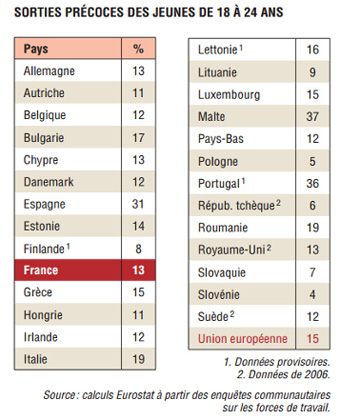
\includegraphics[scale=0.5]{stat12.jpg} 
\end{minipage}

\begin{enumerate}
\item Détermine la médiane des sorties précoces en Europe. 

\item 
\begin{enumerate}
\item Compléter le tableau suivant.

\begin{tabular}{|c|c|c|c|c|c|c|}
\hline 
Sorties précoces en 2007 & [0;5[ & [5;10[ & [10;15[ & [15;20[ & [20;25[ & [25;30] \\ 
\hline 
Effectif de pays européens &  &  &  &  &  &  \\ 
\hline 
E.C.C. des pays européens &  &  &  &  &  &  \\ 
\hline 
\end{tabular} 

\item Construis le polygone des effectifs cumulés croissants.

\item En déduire la médiane des sorties précoces en Europe. 
 
\item Compare avec la question 1.
\end{enumerate}
\end{enumerate}



  
\end{AD}

\begin{DefT}{Etendue}
On appelle \textbf{étendue} d'une série statistique la différence entre la plus grande valeur de la série et la plus petite valeur de la série.
\end{DefT}



\begin{AD}

Lors du devoir commun de Quatrième, voici les résultats de 2 classes.

\begin{minipage}{0.5\linewidth}
\begin{center}
\textbf{Quatrième  1}


\begin{tabular}{|c|c|c|c|c|c|}
\hline 
20 & 18 & 25 & 28& 35 & 27 \\ 
\hline 
22 & 17 & 15 & 26 &37 & 30 \\ 
\hline 
12 & 20 & 21 & 21 & 22 & 30 \\ 
\hline 
30 & 33 & 32 & 23 & 22 & 32 \\ 
\hline 
\end{tabular} 
\end{center}
\end{minipage}
\begin{minipage}{0.5\linewidth}
\begin{center}
\textbf{Quatrième  2}


\begin{tabular}{|c|c|c|c|c|c|}
\hline 
21 & 15 & 25 & 28& 35 & 27 \\ 
\hline 
39 & 9 & 15 & 26 &37 & 30 \\ 
\hline 
15 & 20 & 22 & 21 & 22 & 35 \\ 
\hline 
30 & 30 & 32 & 27 & 29 & 33 \\ 
\hline 
\end{tabular} 
\end{center}
\end{minipage}

\begin{enumerate}
\item Calculer l'étendue de chaque classe.
\item Quelle est la classe la plus hétérogène ?
\item Calculer la médiane de chaque classe.
\item Interpréter les résultats statistiques.
\end{enumerate}
\end{AD}





\begin{autoeval}
\begin{tabular}{p{12cm}p{0.5cm}p{0.5cm}p{0.5cm}p{1cm}}
\textbf{Compétences visées} &  M I & MF & MF  & TBM \vcomp \\ 
Calculer une médiane & $\square$ & $\square$  & $\square$ & $\square$ \\ 
Calculer une étendue & $\square$ & $\square$ & $\square$ & $\square$  \\ 
Interpréter une caractéristique de position& $\square$ & $\square$  & $\square$ & $\square$ \\ 
Interpréter une caractéristique de dispersion & $\square$ & $\square$ & $\square$ & $\square$ \\ 
\end{tabular}
{\footnotesize MI : maitrise insuffisante ; MF = Maitrise fragile ; MS = Maitrise satisfaisante ; TBM = Très bonne maitrise}
 
\end{autoeval} % Auto évaluation
%\begin{titre}[Fonctions de référence]

\Titre{La fonction Cube}{3}
\end{titre}

\begin{CpsCol}
\textbf{Variations de fonctions}
\begin{description}
\item[$\square$] Connaitre la fonction Cube : définition et courbes représentative.
\item[$\square$] Pour la fonction Cube, résoudre graphiquement ou algébriquement une équation ou une inéquation du type $f(x) = k$, $f(x) < k$.
\item[$\square$] Étudier la parité d'une fonction dans des cas simples.
\end{description}
\end{CpsCol}




\begin{DefT}{Fonction Cube}\index{Fonctions!Cube}
La \textbf{fonction Cube} $f$ est la fonction définie sur $\R$ par $f(x)=x^3$.
\end{DefT}

 
\begin{DefT}{Racine cubique}\index{Fonctions!Racine cubique}
La \textbf{racine cubique} de $x$ est le \textit{nombre réel} $a$ tel que $a^3=x$. On note : $a = \sqrt[3]{x}$.
\end{DefT}

\begin{Ex}
\begin{description}
\item[•] La  racine cubique  de $8$ est égale à 2, on écrit que $2 = \sqrt[3]{8}$ ou $2^3 = 8$.
\item[•] La  racine cubique  de $-27$ est égale à $-3$, on écrit que $-3 = \sqrt[3]{-27}$ ou $(-3)^3 = -27$.
\end{description}
\end{Ex}



\begin{Pp}[Variations]
\begin{minipage}{0.48\linewidth}
La fonction Cube est strictement  croissante sur $\R$. La fonction Cube est impaire. Sa courbe représentative est symétrique par rapport à l'origine du repère.
\end{minipage}
\hfill
\begin{minipage}{0.48\linewidth}
\begin{tikzpicture}
\tkzTabInit[lgt=1,espcl=2]{ $x$ / 1,$f $ / 2}
{ $-\infty$ , $+\infty$}
\tkzTabVar{-/$-\infty$ , +/$+\infty$ }
\end{tikzpicture}
\end{minipage}
\end{Pp}

\ROC

\mini{
\EPC{1}{FR-45}{Chercher.}
 
\EPC{1}{FR-46}{Raisonner.}
}{
\EPC{1}{FR-48}{Chercher.}
}


\mini{
\EPC{1}{FR-47}{Représenter.}

\EPC{1}{FR-50}{Représenter. Raisonner. Calculer}
}{
\EPC{1}{FR-49}{Chercher.}

\EPCC{1}{FR-51}{Calculer.}
}





 % La fonction Cube
%\begin{titre}[Géométrie vectorielle et analytique]

\Titre{Notions de vecteur}{4}
\end{titre}

\begin{CpsCol}
\textbf{Connaitre la notion de vecteur}
\begin{description}
\item[$\square$] Représenter géométriquement des vecteurs.
\item[$\square$] Représenter un vecteur dont on connaît les coordonnées. Lire les coordonnées d’un
vecteur.
\end{description}
\end{CpsCol}



\begin{DefT}{Vecteur}\index{Vecteurs}
On dit que le vecteur $\overrightarrow{AB}$ est le représentant du déplacement de A vers B. Le vecteur $\overrightarrow{AB}$ possède donc une \textbf{direction}, un \textbf{sens}, une longueur appelée \textbf{norme}. 
Ces 3 données caractérisent un vecteur.

La translation de vecteur $\overrightarrow{AB}$ est le déplacement de A vers B.
\end{DefT}


 
 
\begin{ThT}{Vecteurs égaux} \index{Vecteurs!Égaux} 
\begin{minipage}{0.48\linewidth}
Deux vecteurs $\overrightarrow{AB}$ et $\overrightarrow{CD}$ sont égaux lorsque ils ont la même direction (leurs supports sont parallèles), le même sens, la même norme $(AB=CD)$.

On écrit $\overrightarrow{AB}=\overrightarrow{CD}$. 

Le quadrilatère $ABDC$ est donc un parallélogramme.
\end{minipage}
\hfill
\begin{minipage}{0.48\linewidth}
\definecolor{ffqqqq}{rgb}{1.,0.,0.}
\definecolor{qqqqff}{rgb}{0.,0.,1.}
\begin{tikzpicture}[line cap=round,line join=round,>=triangle 45,x=1.0cm,y=1.0cm]
\clip(-2.46,-0.22) rectangle (4.58,2.42);
\draw [->,color=ffqqqq] (-2.,0.) -- (1.,2.);
\draw [color=ffqqqq](-0.82,1.46) node[anchor=north west] {$\vec{u}$};
\draw [->,color=ffqqqq] (1.,0.) -- (4.,2.);
\draw [color=ffqqqq](2.06,1.38) node[anchor=north west] {$\vec{v}$};
\begin{scriptsize}
\draw [fill=qqqqff] (-2.,0.) circle (0.5pt);
\draw[color=qqqqff] (-2.24,0.) node {$A$};
\draw [fill=qqqqff] (1.,2.) circle (0.5pt);
\draw[color=qqqqff] (1.14,2.2) node {$B$};
\draw [fill=qqqqff] (1.,0.) circle (0.5pt);
\draw[color=qqqqff] (0.7,-0) node {$C$};
\draw [fill=qqqqff] (4.,2.) circle (0.5pt);
\draw[color=qqqqff] (4.14,2.2) node {$D$};
\end{scriptsize}
\end{tikzpicture}
\end{minipage}
\end{ThT}


\begin{DefT}{Vecteur nul}\index{Vecteurs!Nul}
On dit que le vecteur $\overrightarrow{AB}$ est nul lorsque $A$ et $B$ sont confondus. On note $\overrightarrow{AB}=\overrightarrow{0}$
\end{DefT}




\mini{

\EPC{1}{GVA-32}{Représenter. Raisonner.}

\EPC{1}{GVA-33}{Représenter. Raisonner.}

\EPC{1}{GVA-35}{Représenter. Raisonner.}
}{
\EPC{1}{GVA-34}{Représenter. Calculer.}

\begin{DefT}{Vecteurs opposés}\index{Vecteurs!Opposés}
Deux vecteurs sont dits opposés lorsqu'ils ont la même direction, la même norme et sont de sens opposés. $\overrightarrow{AB}$ et  $\overrightarrow{BA}$ sont opposés. On écrit : $\overrightarrow{AB} = -\overrightarrow{BA}$.
\end{DefT}
}


\EPC{1}{GVA-40}{Représenter}

\begin{DefT}{Base et repère du plan}\index{Base du plan}\index{Repère du plan}
Deux vecteurs non colinéaires forment une \textbf{base} du plan. On le note $\left(\vec{u};\vec{v}\right)$.  \\ 
Deux vecteurs non colinéaires et un point du plan forment un \textbf{repère} du plan. On la note \Oij. Un repère permet de repérer des points dans le plan. Les coordonnées des points sont dépendantes de l'origine $O$.
\end{DefT}




\begin{ThT}{Coordonnées de vecteurs}\index{Vecteurs!Coordonnées}

Deux vecteurs égaux ont des coordonnées égales.
$\overrightarrow{AB}(x,y)$ et $\overrightarrow{CD}(x',y')$.

$\overrightarrow{AB}=\overrightarrow{CD} \Longleftrightarrow x=x'$ et $y=y'$.

Dans un repère on donne deux points $A(x_A; y_A)$ et $B(x_B;y_B)$. Les coordonnées du vecteur $\overrightarrow{AB}$ sont $(x_B – x_A; y_B – y_A)$.
\end{ThT}


\mini{
\EPC{1}{GVA-37}{Représenter}

\EPC{0}{GVA-46}{Représenter. Calculer}
}{
\EPC{1}{GVA-44}{Représenter}

\EPC{0}{GVA-36}{Représenter. Calculer}
}
  % Vecteurs, égalité, Chasles, construction
%\begin{titre}[Fonctions de référence]

\Titre{La fonction Inverse}{4}
\end{titre}



\begin{CpsCol}
\textbf{Variations de fonctions}
\begin{description}
\item[$\square$] Connaitre la fonction Inverse : définition et courbes représentative.
\item[$\square$] Pour la fonction Inverse, résoudre graphiquement ou algébriquement une équation ou une inéquation du type $f(x) = k$, $f(x) < k$.
\item[$\square$] Étudier la parité d'une fonction dans des cas simples.
\end{description}
\end{CpsCol}




\begin{DefT}{Fonction Inverse}\index{Fonctions!Inverse}
La \textbf{fonction Inverse} $f$ est la fonction définie sur $\R^*$ par $f(x)=\frac{1}{x}$.
\end{DefT}


\begin{DefT}{Représentation graphique} \index{Fonction Inverse! Représentation graphique}\index{Hyperbole| see Fonction Inverse! Représentation graphique}
La \textbf{représentation graphique} de la fonction Inverse s'appelle une \textbf{hyperbole} et son équation est $y=\frac{1}{x}$. 
\end{DefT}



\begin{Pp}[Variations]
\begin{minipage}{0.48\linewidth}
La fonction Inverse est strictement décroissante sur $\R^*_-$ et strictement décroissante sur $\R^*_+$. 

L'hyperbole d'équation $y=\frac{1}{x}$ est symétrique par rapport à l'origine du repère.
\end{minipage}
\hfill
\begin{minipage}{0.48\linewidth}
\begin{tikzpicture}
\tkzTabInit[lgt=1,espcl=2]{ $x$ / 1,$f $ / 2}
{ $-\infty$ , $0$ ,$+\infty$}
\tkzTabVar{+/$0$ , -D+ /$ $/$ $ , -/$0$}
\end{tikzpicture}
\end{minipage}
\end{Pp}

\ROC

\mini{
\EPCB{1}{FR-6}{Raisonner.}
 
\EPCB{1}{FR-8}{Raisonner.}

\EPCC{1}{FR-11}{Représenter. Raisonner.}
}{
\EPCB{1}{FR-12}{Représenter. Raisonner.}

\EPCB{1}{FR-19}{Raisonner. Calculer.}
}


\mini{
%\EPCB{1}{FR-13}{Représenter. Raisonner. Calculer}

\EPCB{1}{FR-14}{Représenter. Raisonner. Calculer}

%\EPCB{1}{FR-21}{Représenter. Raisonner. Calculer}
\EPCB{1}{FR-18}{Représenter. Raisonner. Calculer}
}{


\EPCC{1}{FR-16}{Représenter. Raisonner. Calculer}

\EPCC{1}{FR-20}{Représenter. Raisonner. Calculer}
}





 % La fonction Inverse
%\begin{titre}[Probabilités]

\Titre{Probabilité, loi de probabilité}{4}
\end{titre}


\begin{CpsCol}
\begin{description}
\item[$\square$] Utiliser des modèles théoriques de référence (dé, pièce équilibrée, tirage au sort avec
équiprobabilité dans une population) en comprenant que les probabilités sont définies
a priori.
\item[$\square$] Construire un modèle à partir de fréquences observées, en distinguant nettement
modèle et réalité.
\item[$\square$] Calculer des probabilités dans des cas simples : expérience aléatoire à deux ou trois
épreuves.
\end{description}
\end{CpsCol}

\Rec{1}{Prob-20}

\begin{DefT}{Épreuve ou expérience aléatoire}\index{Épreuve}\index{Expérience aléatoire}
On appelle \textbf{épreuve} ou \textbf{expérience aléatoire}, une situation soumise au hasard.

On appelle \textbf{issue} le résultat d'une épreuve, notée $\omega$. 

L'ensemble des issues est l'\textbf{univers}, noté $\Omega$.\index{Univers} \index{Issue}
\end{DefT}

\begin{Ex}
On lance un dé cubique dont les faces sont numérotées de 1 à 6 et on observe le numéro de la face obtenue. Cette expérience a 6 issues possibles dont une issue est le 6. L'univers est $\Omega = \lbrace 1;2;3;4;5;6 \rbrace$.
\end{Ex}



\mini{
\EPC{1}{Prob-6}{Modéliser. Représenter.}
}{
\EPC{0}{Prob-5}{Modéliser. Représenter.}
}


\begin{DefT}{Loi de probabilités}\index{Loi de probabilités}
Définir la loi de probabilité pour une expérience aléatoire dont l'univers est $\Omega = \lbrace x_1; x_2; ... ; x_n \rbrace$ consiste à déterminer pour chacune des issues $x_i$ un nombre $p_i$, $i$ variant de 1 à $n$, appelée \textbf{probabilité}, tel que $p_1+p_2+...p_n=1$
\end{DefT}

\begin{Ex}
On lance un dé cubique équilibré dont les faces sont numérotées de 1 à 6 et on observe le numéro de la face obtenue.   Donc $p_1+p_2+p_3+p_4+p_5+p_6=1$. Comme le dé est équilibré, $p_i=\frac{1}{6}$.
\end{Ex}


\begin{Pp}
En répétant un grand nombre de fois une expérience aléatoire, la fréquence de chaque issue se stabilise autour d'une valeur. Cette valeur est la probabilité de l'issue.
\end{Pp}



\mini{
\EPC{1}{Prob-31}{Communiquer.}
 
\EPC{1}{Prob-26}{Communiquer.}

\EPC{1}{Prob-28}{Modéliser.}

\EPC{1}{Prob-27}{Communiquer.}
}{
\EPC{1}{Prob-32}{Modéliser. }

\EPC{1}{Prob-8}{Chercher.}

\EPC{0}{Prob-18}{Chercher.}

\EPC{0}{Prob-29}{Modéliser.}
}





\EPCP{1}{Prob-25}{Modéliser. Représenter.}

%\EPCP{1}{Prob-0}{Modéliser. Représenter.}

 % Probabilité + Loi de proba
%\begin{titre}[Géométrie vectorielle et analytique]

\Titre{Milieu de segment}{1}
\end{titre}


\begin{CpsCol}
\textbf{Utiliser des nombres pour calculer et résoudre des problèmes}
\begin{description}
\item[$\square$] Calculer les coordonnées du milieu d'un segment
\end{description}
\end{CpsCol}


\Rec{1}{GVA-10}



\begin{Th} \index{Coordonnées du milieu}
\Oij est un repère du plan, $A$ et $B$ deux points de coordonnées $(x_A;y_A)$ et  $(x_B;y_B)$. 

Alors le milieu $M$ du segment $[AB]$ a pour coordonnées $$x_M=\frac{x_A+x_B}{2} ~~ et ~~ y_M=\frac{y_A+y_B}{2}$$

\end{Th}

\mini{
\AD{1}{GVA-15}

\Exo{1}{GVA-20}
}{
\EPC{0}{GVA-18}{Calculer.}
}  % Milieu
%\begin{titre}[Géométrie vectorielle et analytique]

\Titre{Distance entre deux points}{2}
\end{titre}

\begin{CpsCol}
\textbf{Utiliser des nombres pour calculer et résoudre des problèmes}
\begin{description}
\item[$\square$] Calculer la distance entre deux points connaissant les coordonnées des points
\end{description}
\end{CpsCol}



\begin{Th}\index{Distance entre deux points}
\Oij est un repère orthonormal du plan, $A$ et $B$ deux points de coordonnées $(x_A;y_A)$ et  $(x_B;y_B)$. 

Alors la distance $AB$, la longueur du segment $[AB]$, est donnée par  $$d(A,B)=\sqrt{(x_B-x_A)^2+(y_B-y_A)^2}$$
\end{Th}

\mini{
\EPC{1}{GVA-16}{Calculer.}

\EPC{1}{GVA-4}{Raisonner. Représenter. Calculer.}

\EPC{0}{GVA-54}{Raisonner. Représenter. Calculer.}

\EPC{0}{GVA-17}{Raisonner. Représenter. Calculer.}

}{

\EPC{1}{GVA-56}{Modéliser. Représenter. Calculer.}

\EPC{0}{GVA-57}{Raisonner. Calculer.}

\EPC{1}{GVA-19}{Raisonner. Représenter. Calculer.}
}
\newpage
\EPCP{1}{GVA-0}{Raisonner.}   % Distance et coordonnées
%\begin{titre}[Problème du premier degré]

\Titre{Fonctions affines}{3}
\end{titre}


\begin{CpsCol}
\textbf{Variations de fonctions}
\begin{description}
\item[$\square$] Construire une fonction affine pour résoudre un problème
\end{description}
\end{CpsCol}

\Rec{1}{FPD-0}


\begin{DefT}{Fonctions affines}\index{Fonctions!Affine}
Une \textbf{fonction affine} $f$ est une fonction définie sur $\R$ de la forme $f(x)=ax+b$, avec $a\in \R^*$ et $b \in \R$.
\end{DefT}



\begin{Rq}\index{Fonctions!Linéaire}
Une fonction linéaire est une fonction affine particulière ; lorsque $b=0$.
\end{Rq}


\begin{DefT}{Représentation graphique} \index{Fonctions affines! Représentation graphique}
La \textbf{représentation graphique} d'une fonction affine $f$ de la forme $f(x)=ax+b$, avec $a\in \R^*$ et $b \in \R$ est la droite d'équation $y=ax+b$. 
\end{DefT}


\mini{
\EPCN{Modéliser. Représenter. Calculer }


\begin{multicols}{2}
Sur la figure, les droites $(DE)$ et $(BC)$ sont parallèles. $AD=3$, $DB=2$, $AE=4$ et $DE=x$. Soit $f$ la fonction qui à $x$ associe la longueur $BC$. Soit $g$ la fonction qui à $x$ associe le périmètre $AED$ et  $h$ la fonction qui à $x$ associe le périmètre du trapèze $BDEC$.

\begin{center}
\definecolor{xdxdff}{rgb}{0.49019607843137253,0.49019607843137253,1.}
\definecolor{qqqqff}{rgb}{0.,0.,1.}
\begin{tikzpicture}[line cap=round,line join=round,>=triangle 45,x=0.5084745762711864cm,y=0.5084745762711864cm]
\clip(-1.06,-0.36) rectangle (4.92,5.54);
\draw [color=qqqqff] (0.8,5.)-- (0.,0.);
\draw [color=qqqqff] (0.,0.)-- (4.,0.);
\draw [color=qqqqff] (4.,0.)-- (0.8,5.);
\draw [color=qqqqff] (0.3183775351014041,1.9898595943837754)-- (2.72,2.);
\draw (0.2,4.04) node[anchor=north west] {$3$};
\draw (-0.34,1.7) node[anchor=north west] {$2$};
\draw (2.06,3.94) node[anchor=north west] {$4$};
\draw (1.14,2.74) node[anchor=north west] {$x$};
\begin{scriptsize}
\draw [color=qqqqff] (0.8,5.)-- ++(-2.5pt,0 pt) -- ++(5.0pt,0 pt) ++(-2.5pt,-2.5pt) -- ++(0 pt,5.0pt);
\draw[color=qqqqff] (0.94,5.36) node {$A$};
\draw [color=qqqqff] (0.,0.)-- ++(-2.5pt,0 pt) -- ++(5.0pt,0 pt) ++(-2.5pt,-2.5pt) -- ++(0 pt,5.0pt);
\draw[color=qqqqff] (-0.32,0.36) node {$B$};
\draw [color=qqqqff] (4.,0.)-- ++(-2.5pt,0 pt) -- ++(5.0pt,0 pt) ++(-2.5pt,-2.5pt) -- ++(0 pt,5.0pt);
\draw[color=qqqqff] (4.14,0.36) node {$C$};
\draw [color=xdxdff] (0.3183775351014041,1.9898595943837754)-- ++(-2.5pt,0 pt) -- ++(5.0pt,0 pt) ++(-2.5pt,-2.5pt) -- ++(0 pt,5.0pt);
\draw[color=xdxdff] (0.,2.32) node {$D$};
\draw [color=xdxdff] (2.72,2.)-- ++(-2.5pt,0 pt) -- ++(5.0pt,0 pt) ++(-2.5pt,-2.5pt) -- ++(0 pt,5.0pt);
\draw[color=xdxdff] (2.86,2.36) node {$E$};
\end{scriptsize}
\end{tikzpicture}
\end{center}

\end{multicols}

\begin{enumerate}
\item Exprimer $f(x)$, $g(x)$ et $h(x)$ en fonction de $x$. Ces fonctions sont-elles affines ? Linéaires ?
\item En donner des représentations graphiques sur $[1;7]$.
\item En déduire graphiquement la valeur de $x$ pour que $ADE$ et $BDEC$ aient le même périmètre.
\item Retrouver ce résultat par le calcul.
\end{enumerate}


\EPCN{Calculer }


Résoudre dans $\R$ l'équation $4x+2=3-2x$.

Résoudre dans $\R$ l'équation $2(x+3)+1=3-(x-6)$.
}{
\EPCN{Calculer }


\begin{enumerate}
\item Déterminer une fonction affine $f$ telle que $f(0)=5$ et $f(2)=3$.
\item Déterminer une fonction affine $f$ telle que $f(-2)=1$ et $f(3)=6$.
\end{enumerate}


\EPCN{Modéliser. Communiquer. Calculer }


Un cycliste monte une cote de 24 km à la vitesse moyenne de $12 km.h^{-1}$, puis la descend à la vitesse moyenne de $36 km.h^{-1}$.
\begin{enumerate}
\item Soit $d$ la distance parcourue par le cycliste en fonction de la durée $t$ en heures. Écrire $d(t)$ pour $0<t<2$. Pour $t>2$, montrer que $d(t)=24+36(t-2)$.
\item Donner une représentation graphique de $d$
\item Sur le même dessin, donner la représentation de la fonction $h$ qui à $t$ associe la distance qui reste à parcourir en fonction de $t$ pour revenir au départ.
\end{enumerate}
}








% La fonction affine
%\documentclass[10pt]{article}

\input{../../../latex_preambule_style/preambule}
\input{../../../latex_preambule_style/styleCourslycee}
\input{../../../latex_preambule_style/styleExercices}
%\input{../../latex_preambule_style/styleCahier}
\input{../../../latex_preambule_style/bas_de_page_seconde}
\input{../../../latex_preambule_style/algobox}



%%%%%%%%%%%%%%%  Affichage ou impression  %%%%%%%%%%%%%%%%%%
\newcommand{\impress}[2]{
\ifthenelse{\equal{#1}{1}}  %   1 imprime / affiche  -----    0 n'affiche pas
{%condition vraie
#2
}% fin condition vraie
{%condition fausse
}% fin condition fausse
} % fin de la procédure
%%%%%%%%%%%%%%%  Affichage ou impression  %%%%%%%%%%%%%%%%%%



%%%%%%%%%%%%%%%  Indentation  %%%%%%%%%%%%%%%%%%
\parindent=0pt
%%%%%%%%%%%%%%%%%%%%%%%%%%%%%%%%%%%%%%%%%%%%%%%%
\begin{document}

\begin{titre}[Les fonctions de référence]

\Titre{Calculs numériques et algébriques}{3}
\end{titre}


\begin{CpsCol}
\begin{description}
\item[$\square$] Si $a$ et $b$ sont des réels, $(a+b)^2=a^2+2ab+b^2$.
\item[$\square$] Si $a$ et $b$ sont des réels, $(a-b)^2=a^2-2ab+b^2$.
\item[$\square$] Si $a$ et $b$ sont des réels strictement positifs, $\sqrt{a \times b} = \sqrt{a} \times \sqrt{b}$.
\item[$\square$] Étudier la position relative des courbes d’équation $y = x$, $y = x^2$, $y = x^3$, pour $x \geq 0$.
\item[$\square$] Étudier la parité d’une fonction dans des cas simples.
\end{description}
\end{CpsCol}



\EPCN{Calculer}

\begin{enumerate}
\item Développer $(a+b)(a+b)$ où $a$ et $b$ sont deux réels.
\item En déduire la forme développée de $(a+b)^2$. \fbox{Encadrer la formule dans votre cours.}
\item Dans la suite de l'exercice, $x$ est un nombre réel. Utiliser la question précédente pour factoriser les expressions suivantes : 
\begin{enumerate}
\item $A(x)=x^2+2x+1$.
\item $B(x)=x^2+6x+9$.
\item $C(x)=x^2+10x+25$.
\item $D(x)=x^2+20x+100$.
\end{enumerate}
\item Factoriser $H(x)=4x^2+12x+9$ 
\end{enumerate}
 

\EPCN{Calculer}

\begin{enumerate}
\item Développer $(a-b)(a-b)$ où $a$ et $b$ sont deux réels.
\item En déduire la forme développée de $(a-b)^2$. \fbox{Encadrer la formule dans votre cours.}
\item Dans la suite de l'exercice, $x$ est un nombre réel. Utiliser la question précédente pour factoriser les expressions suivantes : 
\begin{enumerate}
\item $A(x)=x^2-2x+1$.
\item $B(x)=x^2-6x+9$.
\item $C(x)=x^2-10x+25$.
\item $D(x)=x^2-20x+100$.
\end{enumerate}
\item Factoriser $H(x)=4x^2-12x+9$ 
\end{enumerate}


\begin{Rq}

$(a+b)^2$ est une forme factorisée puisque $(a+b)^2=(a+b)(a+b)$.

$(a-b)^2$ est une forme factorisée puisque $(a-b)^2=(a-b)(a-b)$.
\end{Rq}

 
\begin{minipage}{0.55\linewidth}
\EPC{1}{FEA-26}{Raisonner. Calculer. }
\end{minipage}
\begin{minipage}{0.45\linewidth}
\EPC{1}{FEA-86}{Représenter. Calculer. }
\end{minipage}




\EPCN{Calculer.}

On pose $x = \sqrt{3}$ et $y=\sqrt{2}$. Calculer

\begin{enumerate}
\begin{minipage}{0.25\linewidth}
\item $A = x^4-y$
\end{minipage}
\begin{minipage}{0.25\linewidth}
\item $B = 2x^2+2x+3$
\end{minipage}
\begin{minipage}{0.25\linewidth}
\item $C = (x+2)(x-4)$
\end{minipage}
\begin{minipage}{0.25\linewidth}
\item $D = x^3 \times y^3$
\end{minipage}
\end{enumerate}



\EPCN{Calculer.}

Le but de cet exercice est de simplifier les écritures numériques.

\begin{Ex}
$\sqrt{12} = \sqrt{4 \times 3} = \sqrt{4} \times \sqrt{3}= 2 \sqrt{3}$

Remarque : $\sqrt{12} = \sqrt{6 \times 2}$ mais ce produit n'aboutit pas.
\end{Ex}
 

\begin{enumerate}
\item Écrire sous la forme $a\sqrt{b}$ les nombres suivants :

$A = \sqrt{8}$ , $B=\sqrt{27}$ , $C=\sqrt{20}$  , $D=\sqrt{18}$  , $E=\sqrt{12}$  , $F=\sqrt{72}$
\item Simplifie les écritures :

$A=\frac{\sqrt{20}}{4}$ , $B = \frac{2-\sqrt{8}}{4}$ , $C=\frac{3-\sqrt{27}}{3}$ , $D=\sqrt{18}\sqrt{2}$  , $E=\sqrt{12}+\sqrt{45}$  , $F=\sqrt{18} -\sqrt{72} +\sqrt{32}$

\end{enumerate}


\EPC{1}{FEA-51}{Calculer.}

\begin{minipage}{0.45\linewidth}
\EPCN{Calculer}

Soit $x \in \R-\left\lbrace 0;-1\right\rbrace $.  Calculer $\frac{1}{x+1}-\frac{1}{x}$

 \end{minipage}
\begin{minipage}{0.55\linewidth}

\EPCN{Raisonner. Calculer.}

Soit $a$ et $b$ deux réels non nuls. Est-il vrai que $\frac{1}{\frac{1}{a}+\frac{1}{b}}=a+b$ ?
 \end{minipage}



\EPCN{Calculer.} 

On donne $E = \frac{2}{3}+\frac{17}{2} \times \frac{4}{3}$ et $F = \frac{\sqrt 6 \times \sqrt 3\times \sqrt{16} }{\sqrt 2}  $ 
 
Démontrer que les nombres E et F sont égaux.



\EPCN{Représenter. Calculer.}

Soit $x \geq 0$.
\begin{enumerate}
\item Étudier le signe de $x^3-x^2$.
\item Étudier le signe de $x^2-x$.
\item En déduire la position relative des courbes d’équation $y = x$, $y = x^2$, $y = x^3$, pour $x \geq 0$.
\end{enumerate}
\textit{Aide : Penser à factoriser. On pourra utiliser sa calculatrice ou Geogebra pour visualiser les courbes.}


\EPCN{Représenter. Calculer.}

\begin{enumerate}
\item 
\begin{enumerate}
\item Soit $f$ la fonction Carré. Calculer $f(-x)$. Comparer $f(-x)$ et $f(x)$. On dit que la fonction est paire.
\item Soit $g$ la fonction Cube. Calculer $g(-x)$. Comparer $g(-x)$ et $g(x)$. On dit que la fonction est impaire.
\item Soit $i$ la fonction Inverse. Calculer $i(-x)$. Comparer $i(-x)$ et $i(x)$. Que dire de la fonction inverse ?
\item La fonction Racine carrée est-elle paire ? impaire ? justifier.
\end{enumerate}
\item La fonction $h$ définie sur $\R$ par $h(x)=x^2+2$ est-elle paire ? impaire ? justifier.
\item La fonction $k$ définie sur $\R$ par $k(x)=x^3+x-2$ est-elle paire ? impaire ? justifier.
\item La fonction $u$ définie sur $\R$ par $u(x)=x^3+x^2-2$ est-elle paire ? impaire ? justifier.
\end{enumerate}
 
\newpage

\begin{titre}[Les fonctions de référence]

\Titre{Calculs algébriques}{1}
\end{titre}

\begin{CpsCol}
\begin{description}
\item[$\square$] Résoudre algébriquement une équation ou une inéquation du type $f(x) = k$, $f(x) < k$.
\end{description}
\end{CpsCol}


 
\begin{minipage}{0.55\linewidth}
\EPCN{Calculer }

Résoudre les équations suivantes dans $\R$.

\begin{enumerate}
\item $(x+3)(x-7)=0$
\item $x^3-x=0$
\item $\left( x-\sqrt{3} \right)(5-2x)=0$
\end{enumerate}

 \end{minipage}
\begin{minipage}{0.55\linewidth}
\EPCN{Calculer }

Résoudre les inéquations suivantes dans $\R$.

\begin{enumerate}
\item $2x+1>3$
\item $-5x + \frac{1}{2} \geq \frac{5}{2}$
\end{enumerate}
 \end{minipage}

\EPCN{Représenter. Raisonner. Calculer }

On considère un triangle $ABC$ et un nombre réel $x$. On a $AB=x+1$, $BC=4$ et $CA=15$.

\begin{enumerate}
\item Montrer que $x+1 \leq 19$ et $ x+5 > 15$
\item Donner le plus grand intervalle de $\R$ auquel appartient $x$.
\end{enumerate}




\EPCN{ Représenter. Calculer. }

On souhaite démontrer que $x^3-8=0$ n'admet qu'une unique solution $x=2$ sur $\R$.

\begin{enumerate}
\item Démontrer que pour tout réel $x$, $x^3-8=(x-2)(x^2+2x+4)$.
\item
\begin{enumerate}
\item Démontrer que pour tout réel $x$, $x+2x+4=(x+1)^2+3$.
\item En déduire que pour tout réel $x$, $x+2x+4>0$.
\end{enumerate}
\item En déduire que $x^3-8=0$ n'admet qu'une unique solution $x=2$ sur $\R$. 
\end{enumerate}



\EPCN{ Représenter. Calculer. }

\begin{enumerate}
\item Résoudre, $\sqrt{x^2-3}=1$.
\item Résoudre, $\sqrt{x-3}=x+1$. 
\item Résoudre, $\frac{3}{x}=4$. 
\item Résoudre, $\frac{-1}{x}=x+2$. 
\item Résoudre, $\sqrt{x}-x=0$. 
\end{enumerate}




\EPCN{ Raisonner. Calculer. }

Soit $k$ un nombre réel. On considère l'équation suivante d'inconnue $x$ : $k^2x+7=x-2k$.


\begin{enumerate}
\item Résoudre cette équation dans $\R$ en fonction de $k$.
\item Pour quelles valeurs de $k$ n'existe-t-il pas de solution ?
\item A quel plus petit ensemble de nombres appartient $k$ lorsque 0 est une solution de l'équation ?
\end{enumerate}
%
%
%
%
%
%\begin{minipage}{0.56\linewidth}
%
%
%\EPC{1}{FR-45}{Chercher.}
%
%
Ranger \textbf{sans calculatrice} par ordre croissant les nombres suivants :

 $\sqrt{3}$; $\sqrt{\frac{5}{3}}$; $\sqrt{\pi}$; $ \sqrt{3,8}$ ; $ \sqrt{0,1287}$

 
%
%Justifier votre démarche dans chaque cas.
%
%\EPC{1}{FR-47}{Représenter.}
%\end{minipage}
%\hfill
%\begin{minipage}{0.42\linewidth}
%
%\EPC{1}{FR-57}{Représenter.} 
%\end{minipage}
%
%
%\EPC{1}{FPD-0}{Chercher. Représenter.}
%
%\EPC{1}{FPD-2}{Chercher. Représenter.}
%
%\EPC{1}{FR-56}{Calculer}
%
%\EPC{1}{FR-51}{Chercher.}
%
%\EPC{1}{FR-54}{Calculer.}
% 
%\EPC{1}{FR-6}{Raisonner. Communiquer.}
%
%\begin{minipage}{0.49\linewidth}
%\EPC{1}{FR-55}{Représenter.} 
%\end{minipage}
%\hfill
%\begin{minipage}{0.49\linewidth}
%\EPC{1}{FR-62}{Représenter.} 
%\end{minipage}
%
%\EPC{1}{FR-63}{Représenter.} 
%
%\EPC{1}{FR-61}{Chercher. Raisonner.}
% 
%
%\EPCC{1}{FR-58}{Raisonner. Communiquer.}
%
%\EPCC{1}{FR-59}{Raisonner. Communiquer.}
%
%\EPCC{1}{FR-60}{Raisonner. Communiquer.}


%\EPC{1}{stat-35}{Chercher. Modéliser.}
%
%\ligne{30}
% 
%\multido{\i=0+1}{87}{ \AD{1}{FEA-\i} }
\end{document}

%\begin{titre}[Calcul littéral]

\Titre{Résolution d'équation, d'inéquation}{3}
\end{titre}

\begin{CpsCol}
\begin{description}
\item[$\square$] Modéliser un problème par une inéquation.
\item[$\square$] Résoudre une équation, une inéquation du premier degré
\end{description}
\end{CpsCol}



\begin{minipage}{0.48\linewidth}

\EPCN{Calculer }

Résoudre les équations suivantes dans $\R$.

\begin{enumerate}
\item $3x+7=0$
\item $3(x+7)=9$
\item $5x-4=2x+2$
\item $2(x-4)=3(5-2x)+1$
\end{enumerate}

\end{minipage}
\hfill
\begin{minipage}{0.48\linewidth}

\EPCNM{Calculer }

Résoudre les équations suivantes dans $\R$.

\begin{enumerate}
\item $(x+3)(x-7)=0$
\item $x^3-x=0$
\item $(x-3)(2-x)=0$
\item $\left( x-\sqrt{3} \right)(5-2x)=0$
\end{enumerate}
\end{minipage}

\EPCN{Représenter. Calculer. Communiquer. }

La somme de trois nombres entiers consécutifs est égale à 147. Quels sont ces trois nombres ?


\begin{minipage}{0.48\linewidth}

\EPCNM{Représenter. Raisonner. Calculer }

Résoudre les équation suivantes dans $\R$ : 

\begin{enumerate}
\item $(x+3)^2=x(x+3)$.
\item $\frac{2}{5}x+8=\frac{1}{3}(x-7)$.
\end{enumerate}
\end{minipage}
\hfill
\begin{minipage}{0.48\linewidth}

\EPCN{Calculer }

Résoudre les inéquations suivantes dans $\R$.

\begin{enumerate}
\item $2x+1>3$
\item $3x-2 \leq 7$
\item $-5x + \frac{1}{2} \geq \frac{5}{2}$
\item $2(x-4) > 3(5-2x)+1$
\end{enumerate}


\end{minipage}


\EPCN{Représenter. Raisonner. Calculer }

On considère un triangle $ABC$ et un nombre réel $x$. On a $AB=x+1$, $BC=4$ et $CA=15$.

\begin{enumerate}
\item Montrer que $x+1 \leq 19$ et $ x+5 > 15$
\item Donner le plus grand intervalle de $\R$ auquel appartient $x$.
\end{enumerate}


\EPCN{ Raisonner. Calculer }

Soit $k$ un nombre réel. On considère l'équation suivante d'inconnue $x$ : $k^2x+7=x-2k$.

\begin{enumerate}
\item Résoudre cette équation dans $\R$ en fonction de $k$.
\item Pour quelles valeurs de $k$ n'existe-t-il pas de solution ?
\item A quel plus petit ensemble de nombres appartient $k$ lorsque 0 est une solution de l'équation ?
\end{enumerate}


\EPCN{ Raisonner. Calculer }

Soit $m$ un nombre réel. On considère l'équation suivante d'inconnue $m$ : $5mx+7 = x+m$.

Résoudre cette équation dans $\R$ et discuter l'existence de solution selon la valeur de $m$.



\EPCN{ Raisonner. Représenter. Calculer }

On considère un triangle $ABC$ tel que $AB = x+9$, $AC= 2x-1$ et $BC = 3x+6$.

\begin{enumerate}
\item Pour quelle valeurs de $x$, le triangle $ABC$ est-il isocèle en $A$ ?
\item Existe-t-il un réel $x$ tel que le triangle $ABC$ est équilatéral ?
\end{enumerate}
 % Résolution d'équations et d'inéquations
%
%\begin{titre}[Fonctions de référence]

\Titre{La fonction Racine carrée}{2}
\end{titre}


 
\begin{CpsCol}
\textbf{Variations de fonctions}
\begin{description}
\item[$\square$] Connaitre la fonction Racine carrée : définition et courbes représentative.
\item[$\square$] Pour la fonction Racine carrée, résoudre graphiquement ou algébriquement une équation ou une inéquation du type $f(x) = k$, $f(x) < k$.
\end{description}
\end{CpsCol}




\begin{DefT}{Fonction Racine carrée}\index{Fonctions!Racine carrée}
La \textbf{fonction Racine carrée} $f$ est la fonction définie sur $\R^+$ par $f(x)=\sqrt x$.
\end{DefT}

 



\begin{Pp}[Variations]
\begin{minipage}{0.48\linewidth}
La fonction Racine carrée est strictement  croissante sur $\R^+$.  
\end{minipage}
\hfill
\begin{minipage}{0.48\linewidth}
\begin{tikzpicture}
\tkzTabInit[lgt=1,espcl=2]{ $x$ / 1,$f $ / 2}
{ $0$ , $+\infty$}
\tkzTabVar{-/$0$ , +/$+\infty$ }
\end{tikzpicture}
\end{minipage}
\end{Pp}

\ROC

\mini{
\EPC{1}{FR-56}{Calculer}

\EPC{1}{FR-52}{Raisonner.}

\EPC{1}{FR-54}{Calculer.}
}{
\EPC{1}{FR-53}{Chercher.}

\EPC{1}{FR-55}{Représenter.}

\EPC{1}{FR-51}{Chercher.} 
}
% La fonction Racine Carrée 
%\begin{titre}[Calculs numériques]

\Titre{Les racines carrées}{3}
\end{titre}

\begin{CpsCol}
\begin{description}
\item[$\square$] Manipuler les racines carrées
\end{description}
\end{CpsCol}

\begin{DefT}{La racine Carrée}
 Soit $a$ un nombre positif, la racine Carrée de $a$ notée, $\sqrt{a}$, est l'unique nombre positif tel que $\sqrt{a}^2=a$.
\end{DefT}  


\begin{ThT}{Les racines carrées\index{Racines carrées}}
Pour tous nombres $a$ et $b$ positifs, 
\begin{description}
\item $\sqrt{ab}=\sqrt{a}\sqrt{b}$
\item $\sqrt{\frac{a}{b}}=\frac{\sqrt{a}}{\sqrt{b}}$, $b >0$
\end{description}
\end{ThT}

\EPCN{Calculer }

On pose $x = \sqrt{3}$ et $y=\sqrt{2}$. Calculer

\begin{enumerate}
\begin{minipage}{0.5\linewidth}
\item $x^4-y$
\item $2x^2+2x+3$
\end{minipage}
\begin{minipage}{0.5\linewidth}
\item $(x+2)(x-4)$
\item $x^3 \times y^3$
\end{minipage}
\end{enumerate}

\EPCN{Raisonner. Calculer }

\begin{enumerate}
\item Écrire sous la forme $a\sqrt{b}$ les nombres suivants :

$A = \sqrt{8}$ , $B=\sqrt{27}$ , $C=\sqrt{20}$  , $D=\sqrt{18}$  , $E=\sqrt{12}$  , $F=\sqrt{72}$
\item Simplifie les écritures :

$A=\frac{\sqrt{20}}{4}$ , $B = \frac{2-\sqrt{8}}{4}$ , $C=\frac{3-\sqrt{27}}{3}$ , $D=\sqrt{18}\sqrt{2}$  , $E=\sqrt{12}+\sqrt{45}$  , $F=\sqrt{18} -\sqrt{72} +\sqrt{32}$

\end{enumerate}

 

\EPC{0}{FEA-3}{Représenter. Chercher.}
 

 
\EPC{1}{FEA-51}{Calculer }

\EPCN{Raisonner. Représenter. Calculer }

\begin{enumerate}
\item
\begin{enumerate}
\item Tracer un carré $ABCD$ de coté $a$.  
\item Calculer la longueur de la diagonale $AC^2=2a$.
\item En déduire que $AC=a\sqrt{2}$
\end{enumerate}
\item
Applications : 
\begin{enumerate}
\item Quelle est la longueur de la diagonale d'un carré de coté 5 ?
\item Quelle est la longueur de l'hypoténuse d'un triangle isocèle rectangle dont un coté mesure 3cm ?
\end{enumerate}
\end{enumerate}



\EPCN{ Calculer }

On considère un triangle ABC dont les cotés mesurent :$AB = 4\sqrt{3}$, $BC = 2\sqrt{12}$ et $CA= 4\sqrt{6}$. Quelle est la nature de ce triangle ?






\EPCNM{Raisonner. Représenter. Calculer } 

\begin{enumerate}
\item Tracer un triangle équilatéral $ABC$ de coté $a$. $I$ est le milieu de $[AB]$. 
\item Quelle est la longueur $AI$ ?
\item Démontrer que $IC^2=\frac{3a^2}{4}$.
\item Démontrer que la hauteur d'un triangle équilatéral est égale à $\frac{a\sqrt3}{2}$.
\item Quelle est la longueur de la hauteur d'un triangle équilatéral de coté 6 ?
\end{enumerate}



\EPCNM{Raisonner. Représenter. Calculer } 

 
On donne le cube $ABCDEFGH$ suivant de coté de longueur $a$. I est le milieu de $[AB]$. Calculer la longueur $IH$ en fonction de $a$.

\begin{tikzpicture}[line cap=round,line join=round,>=triangle 45,x=1.0cm,y=1.0cm]
\clip(-0.48,-3.68) rectangle (5.76,2.52);
\draw [line width=2.pt] (0.,-3.)-- (4.,-3.);
\draw [line width=2.pt] (4.,-3.)-- (5.,-2.);
\draw [line width=2.pt,dash pattern=on 3pt off 3pt] (5.,-2.)-- (1.,-2.);
\draw [line width=2.pt,dash pattern=on 3pt off 3pt] (1.,-2.)-- (0.,-3.);
\draw [line width=2.pt] (0.,1.)-- (4.,1.);
\draw [line width=2.pt] (4.,1.)-- (5.,2.);
\draw [line width=2.pt] (5.,2.)-- (1.,2.);
\draw [line width=2.pt] (1.,2.)-- (0.,1.);
\draw [line width=2.pt] (0.,1.)-- (0.,-3.);
\draw [line width=2.pt,dash pattern=on 3pt off 3pt] (1.,-2.)-- (1.,2.);
\draw [line width=2.pt] (4.,1.)-- (4.,-3.);
\draw [line width=2.pt] (5.,-2.)-- (5.,2.);
\draw [line width=2.pt,dash pattern=on 3pt off 3pt] (1.,2.)-- (2.,-3.);
\draw [line width=2.pt] (0.,-3.)-- (2.,-3.);
\draw [line width=2.pt] (1.,-2.88) -- (1.,-3.12);
\draw [line width=2.pt] (2.,-3.)-- (4.,-3.);
\draw [line width=2.pt] (3.,-2.88) -- (3.,-3.12);
\begin{scriptsize}
\draw [color=black] (0.,-3.)-- ++(-2.5pt,0 pt) -- ++(5.0pt,0 pt) ++(-2.5pt,-2.5pt) -- ++(0 pt,5.0pt);
\draw[color=black] (-0.3,-2.69) node {$A$};
\draw [color=black] (4.,-3.)-- ++(-2.5pt,0 pt) -- ++(5.0pt,0 pt) ++(-2.5pt,-2.5pt) -- ++(0 pt,5.0pt);
\draw[color=black] (4.18,-3.11) node {$B$};
\draw [color=black] (5.,-2.)-- ++(-2.5pt,0 pt) -- ++(5.0pt,0 pt) ++(-2.5pt,-2.5pt) -- ++(0 pt,5.0pt);
\draw[color=black] (5.14,-1.63) node {$C$};
\draw [color=black] (1.,-2.)-- ++(-2.5pt,0 pt) -- ++(5.0pt,0 pt) ++(-2.5pt,-2.5pt) -- ++(0 pt,5.0pt);
\draw[color=black] (0.72,-1.73) node {$D$};
\draw [color=black] (0.,1.)-- ++(-2.5pt,0 pt) -- ++(5.0pt,0 pt) ++(-2.5pt,-2.5pt) -- ++(0 pt,5.0pt);
\draw[color=black] (-0.16,1.27) node {$E$};
\draw [color=black] (4.,1.)-- ++(-2.5pt,0 pt) -- ++(5.0pt,0 pt) ++(-2.5pt,-2.5pt) -- ++(0 pt,5.0pt);
\draw[color=black] (3.84,1.37) node {$F$};
\draw [color=black] (5.,2.)-- ++(-2.5pt,0 pt) -- ++(5.0pt,0 pt) ++(-2.5pt,-2.5pt) -- ++(0 pt,5.0pt);
\draw[color=black] (5.14,2.37) node {$G$};
\draw [color=black] (1.,2.)-- ++(-2.5pt,0 pt) -- ++(5.0pt,0 pt) ++(-2.5pt,-2.5pt) -- ++(0 pt,5.0pt);
\draw[color=black] (1.14,2.37) node {$H$};
\draw [color=black] (2.,-3.)-- ++(-2.5pt,0 pt) -- ++(5.0pt,0 pt) ++(-2.5pt,-2.5pt) -- ++(0 pt,5.0pt);
\draw[color=black] (2.26,-3.21) node {$I$};
\end{scriptsize}
\end{tikzpicture}



\EPCNA{Raisonner. Représenter. Calculer } 

 
On donne la pyramide à base carrée $ABCD$ de coté de longueur $a$ et de sommet $S$ dont la hauteur est 10 cm.
Pour quelles valeurs de $a$, on a $15 < SA < 20$ ?


\begin{ThT}{Les racines carrées\index{Racines carrées}}
Pour tout nombre $a$, $\sqrt{a^2}= \vert a \vert$
\end{ThT}

\EPCNA{Calculer } 

On donne $E = \frac{2}{3}+\frac{17}{2} \times \frac{4}{3}$ et $F = \frac{\sqrt 6 \times \sqrt 3\times \sqrt{16} }{\sqrt 2}  $ 
 
Démontrer que les nombres E et F sont égaux
 % Racines carrées
\begin{titre}[Informations chiffrées]

\Titre{Évolutions successives}{4}
\end{titre}


\begin{CpsCol}
\begin{description}
\item[$\square$] Exploiter la relation entre deux valeurs successives et leur taux d'évolution.
\item[$\square$] Calculer le taux d'évolution global à partir des taux d'évolution successifs. Calculer un taux d'évolution réciproque.
\end{description}
\end{CpsCol}

 

\begin{DefT}{Évolutions successives}\index{Évolutions! successives}
Lorsqu'une quantité subit des évolutions successives $t_1$, $t_2$, $t_3$, ...de sa valeur initiale, cette quantité subit une évolution globale $t$.
\end{DefT}

\begin{Ex}
 Chaque année, le prix de l'électricité en France augmente d'un certain pourcentage. Le prix de l'électricité a augmenté de 5,9\% le 1er juin 2019 et il avait augmenté de  2,8\% le 1er juin 2018.
\end{Ex}

\begin{ThT}{Taux global d'évolution}
Le taux global d'évolution correspondant à deux évolutions successives de taux respectifs $t_1$ et $t_2$  est le réel $t$ tel que $1+t = \left(1+t_1\right)\left(1+ t_2 \right)$.
\end{ThT}


\begin{Ex}
Dans l'exemple précédent, le prix de l'électricité a augmenté de 5,9\% le 1er juin 2019 et augmenté de  2,8\% le 1er juin 2018.

$t_1=5,9\%=\frac{5,9}{100}$ et $t_2=2,8\%=\frac{2,8}{100}$

donc $1+t = \left(1+\frac{2,8}{100}\right)\left(1+ \frac{5,9}{100} \right)$.
 
$1+t = 1,028 \times 1,059 \approx 1,088$ donc $t = 1,088 - 1 \approx 0,088$ ou $t \approx \frac{8,8}{100}$ ou aussi, $t\approx 8,8\%$.
\end{Ex}




\begin{Rq}
On peut faire correspondre un coefficient multiplicateur global, $CM_g$, au taux global d'évolution tel que $$CM = \left(1+t_1\right)\left(1+t_2\right)$$
\end{Rq}


\begin{Ex}
Un objet A coute 75 euros initialement en 2015. En 2016, cet objet a augmenté de 5\% et son prix a baissé en 2017 de 4\%. Le coefficient multiplicateur global est donc $CM = \left(1+\frac{5}{100}\right)\left(1-\frac{4}{100}\right)=1,05 \times 0,96 = 1,008$.\\
Le taux de pourcentage est donc égal à $0,008 \times 100 = 0,8$. Sur les 2 années, l'objet a augmenté de 0,8\%. 
\end{Ex}


\begin{Dem}
Soit deux taux respectifs $t_1$ et $t_2$. On appelle $CM_1 = 1+t_1$ et $CM_2 = 1+t_2$.\\
Soit $P_0$ la valeur initiale. Après la première évolution, $P_1=CM_1 \times P_0 = \left(1+t_1\right)\times P_0 $\\
Après la seconde évolution, $P_2=CM_2 \times P_1 = CM_2 \times CM_1 \times P_0 =\left(1+t_2\right)\times \left(1+t_1 \right)\times P_0 $.\\
Après les 2 évolutions, $P_2=\left(1+t_2\right)\times \left(1+t_1\right)\times P_0 $. Donc Le coefficient multiplicateur global est $CM = \left(1+t_1\right)\left(1+t_2\right)$.
\end{Dem}

\begin{ThT}{Taux global d'évolution pour $n$ évolutions}
Le taux global d'évolution correspondant à $n$ évolutions successives de taux respectifs $t_1$, $t_2$, $t_3$, ..., $t_n$ est le réel $t$ tel que $$1+t = \left(1+t_1\right)\left(1+t_2\right)\left(1+t_3\right)\cdots \left(1+t_n\right)$$
\end{ThT}

\begin{Rq}
On peut faire correspondre un coefficient multiplicateur global, $CM_g$, au taux global d'évolution tel que $$CM = \left(1+t_1\right) \left(1+t_2\right)\left(1+t_3\right)\cdots \left(1+t_n\right)$$
\end{Rq}

\begin{Ex}
Un article subit les évolutions suivantes lors des 3 dernières années : 3\% en 2015, $-1$\% en 2016 et 2\% en 2017. Quel est le taux global d'évolution sur ces 3 années ?

Le taux d'évolution global est : $CM_g=(1+0,03)(1-0,01)(1+0,02)=1,03 \times 0,99 \times 1,02 = 1,04$ arrondi à 0,01 près.

On peut donc dire que sur les 3 dernières années, l'article a augmenté de 4\%.
\end{Ex}



\mini{
\EPC{1}{IC-34}{Chercher.}

%\EPC{1}{IC-16}{Chercher.}
\EPC{1}{IC-36}{Chercher.}


\EPC{0}{IC-5}{Chercher.}
}{
\EPC{1}{IC-33}{Chercher.}

\EPC{1}{IC-3}{Chercher.}
}


\EPC{0}{IC-9}{Chercher.}




\begin{DefT}{Évolution réciproque}\index{Évolution! réciproque}
Une quantité non nulle $V_i$ subit une évolution de taux $t$ et devient égale à une quantité $V_f$. 

Le \textbf{taux réciproque} de $t$ est le taux d'évolution $t'$ qui permet de passer de $V_f$ à $V_i$.
\end{DefT}


\begin{Ex}
\begin{minipage}{0.7\linewidth}
 
Un objet A coute 50 euros (valeur initiale). Une baisse de 20\% fait passer son prix à 40 euros(valeur finale). Le taux d'évolution $t$ est donc égal à $-20$\%.  

Le taux réciproque $t'$ est le taux qui fait passer de 40 euros (la valeur du prix finale) à 50 euros (la valeur du prix initiale). Donc $t'=\frac{50}{40}=1,25$ donc $t' =+25\%$.
\end{minipage}
\begin{minipage}{0.4\linewidth}
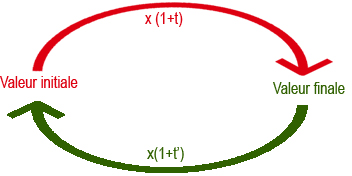
\includegraphics[scale=0.5]{taux_reciproque.jpg} 
\end{minipage}

\end{Ex}


\begin{ThT}{Taux d'évolution réciproque}
\begin{minipage}{0.74\linewidth}
 Le coefficient multiplicateur réciproque $CM'$ associe à l'évolution réciproque $t'$ est l'inverse du coefficient multiplicateur non nul $CM$ associé à l'évolution de départ $t$. 
 
 On a : $CM' = \frac{1}{CM}$ c'est à dire : $CM \times CM' = 1$ 

\end{minipage}
\hfill
\begin{minipage}{0.25\linewidth}

\includegraphics[scale=0.5]{taux_reciproque2.png} 
\end{minipage}
\end{ThT}

\ROC





\begin{Rq}
Le taux réciproque $t'$ n'est pas égal au taux initial $t'$.
\end{Rq}
 


\mini{
\EPC{1}{IC-39}{Chercher.}

\EPC{1}{IC-7}{Chercher.}

\EPCP{1}{IC-40}{Chercher.}
}{
\EPC{1}{IC-35}{Chercher.}

\EPC{0}{IC-37}{Chercher.}
 
\EPC{1}{IC-38}{Chercher.} 
}
 
 % Evolutions successives
%\begin{titre}[Géométrie vectorielle et analytique]

\Titre{Opérations de vecteur}{4}
\end{titre}

\begin{CpsCol}
\textbf{Calculer avec les vecteurs}
\begin{description}
\item[$\square$] Calculer les coordonnées d’une somme de vecteurs, d’un produit d’un vecteur par un
nombre réel.
\item[$\square$] Multiplier un vecteur par un réel
\end{description}
\end{CpsCol}




\begin{DefT}{Somme de deux vecteurs}\index{Vecteurs!Somme}
\begin{minipage}{0.48\linewidth}
Soit $\overrightarrow{u}$ et $\overrightarrow{v}$ deux vecteurs quelconques.

On appelle somme de vecteurs $\overrightarrow{u}$ et $\overrightarrow{v}$, notée $\overrightarrow{u}+\overrightarrow{v}$, le vecteurs $\overrightarrow{w}$ qui résulte de la translation suivant $\overrightarrow{u}$ puis de la translation suivant $\overrightarrow{v}$.
\end{minipage}
\hfill
\begin{minipage}{0.48\linewidth}
\definecolor{qqqqff}{rgb}{0.,0.,1.}
\definecolor{ffqqqq}{rgb}{1.,0.,0.}
\begin{tikzpicture}[line cap=round,line join=round,>=triangle 45,x=1.0cm,y=1.0cm]
\clip(-2.08,-1.32) rectangle (4.12,2.3);
\draw [->,color=ffqqqq] (-2.,-1.) -- (1.,2.);
\draw [->,color=qqqqff] (1.,2.) -- (4.,0.);
\draw [->] (-2.,-1.) -- (4.,0.);
\draw [color=ffqqqq](-0.82,1.26) node[anchor=north west] {$\vec{u}$};
\draw [color=qqqqff](2.64,1.76) node[anchor=north west] {$\vec{v}$};
\draw (0.96,-0.36) node[anchor=north west] {$\vec{w}$};
\end{tikzpicture}
\end{minipage}
\end{DefT}


\begin{Nt}
$\overrightarrow{w}=\overrightarrow{u}+\overrightarrow{v}$
\end{Nt}





\begin{DefT}{Relation de Chasles}\index{Relation de Chasles}
Soit $A$, $B$ et $C$trois points quelconques.

$\overrightarrow{AC}=\overrightarrow{AB}+\overrightarrow{BC}$
\end{DefT}

\mini{
\AD{1}{GVA-22}
}{
\EPC{0}{GVA-50}{Raisonner. Calculer}
}

\begin{Th}
Soit $A$, $B$ et $C$trois points quelconques.\\
Le quadrilatère $ABDC$ est un parallélogramme si et seulement si $\overrightarrow{AD}=\overrightarrow{AB}+\overrightarrow{AC}$.
\end{Th}

\ROC

\begin{Th}

Soit $\overrightarrow{u}$ de coordonnées $(x,y)$ et $\overrightarrow{v}$ de coordonnées $(x',y')$.

Le vecteur  $\overrightarrow{u}+\overrightarrow{v}$ a pour coordonnées $(x+x',y+y')$.
\end{Th}


\mini{
\EPC{1}{GVA-31}{Raisonner. Calculer}

\EPC{1}{GVA-47}{Raisonner. Calculer}
}{
\EPC{1}{GVA-49}{Calculer}
}


\begin{DefT}{Différence de deux vecteurs}\index{Vecteurs!Différence}
\begin{minipage}{0.48\linewidth}
Soit $\overrightarrow{u}$ et $\overrightarrow{v}$ deux vecteurs quelconques.

On appelle \textbf{différence de vecteurs} $\overrightarrow{u}$ et $\overrightarrow{v}$, notée $\overrightarrow{u}-\overrightarrow{v}$, le vecteurs $\overrightarrow{w}$ qui résulte de la translation suivant $\overrightarrow{u}$ puis de la translation suivant $-\overrightarrow{v}$.

\end{minipage}
\hfill
\begin{minipage}{0.48\linewidth}
\definecolor{qqqqff}{rgb}{0.,0.,1.}
\definecolor{qqwuqq}{rgb}{0.,0.39215686274509803,0.}
\definecolor{ffqqqq}{rgb}{1.,0.,0.}
\begin{tikzpicture}[line cap=round,line join=round,>=triangle 45,x=1.0cm,y=1.0cm]
\clip(-2.3,-2.3) rectangle (6.24,2.2);
\draw [->,color=ffqqqq] (-2.,-1.) -- (1.,2.);
\draw [color=ffqqqq](0.42,0.94) node[anchor=north west] {$\vec{u}$};
\draw [->,color=qqwuqq] (6.,1.) -- (4.,2.);
\draw [color=qqwuqq](5.06,2.18) node[anchor=north west] {$\vec{v}$};
\draw [->,color=ffqqqq] (-1.,-2.) -- (2.,1.);
\draw [->,color=qqwuqq] (2.,1.) -- (4.,0.);
\draw [color=qqwuqq](2.64,1.26) node[anchor=north west] {$-\vec{v}$};
\draw [->,color=qqqqff] (-1.,-2.) -- (4.,0.);
\draw [color=qqqqff](1.52,-0.78) node[anchor=north west] {$\vec{u}-\vec{v}$};
\end{tikzpicture}
\end{minipage}
\end{DefT}

\begin{Th}

Soit $\overrightarrow{u}$ de coordonnées $(x,y)$ et $\overrightarrow{v}$ de coordonnées $(x',y')$.

Le vecteur  $\overrightarrow{u}-\overrightarrow{v}$ a pour coordonnées $(x-x',y-y')$.
\end{Th}

\mini{
\AD{1}{GVA-38}
}{
\Exo{1}{GVA-52}

\PO{1}{GVA-41}
}

\begin{DefT}{Produit d'un vecteur par un réel}\index{Vecteurs!Produit d'un vecteur par un réel}
\begin{minipage}{0.48\linewidth}
Soit $\overrightarrow{u}$ un vecteur quelconque et $k$ un réel non nul.

On appelle \textbf{produit du vecteur} $\overrightarrow{u}$ par le réel $k$, le vecteur $k\overrightarrow{u}$ :
\begin{description}
\item[•] de même direction que $\overrightarrow{u}$
\item[•] 
\begin{description}
\item[•] de même sens que $\overrightarrow{u}$ si $k$ est positif
\item[•] de sens opposé à $\overrightarrow{u}$ si $k$ est négatif
\end{description}
\item[•] de norme
\begin{description}
\item[•] $k \times \Vert \overrightarrow{u} \Vert$ si $k$ est positif
\item[•] $-k \times \Vert \overrightarrow{u} \Vert$ si $k$ est négatif
\end{description}

\end{description}

\end{minipage}
\hfill
\begin{minipage}{0.48\linewidth}

\definecolor{ffxfqq}{rgb}{1.,0.4980392156862745,0.}
\definecolor{qqqqff}{rgb}{0.,0.,1.}
\definecolor{ffqqqq}{rgb}{1.,0.,0.}
\begin{tikzpicture}[line cap=round,line join=round,>=triangle 45,x=1.0cm,y=1.0cm]
\clip(-2.1,-1.26) rectangle (4.52,2.16);
\draw [->,color=ffqqqq] (-2.,-1.) -- (1.,2.);
\draw [color=ffqqqq](0.08,1.24) node[anchor=north west] {$\vec{u}$};
\draw [->,color=qqqqff] (1.,0.) -- (2.,1.);
\draw [->,color=ffxfqq] (4.,1.) -- (2.,-1.);
\draw [color=qqqqff](0.34,0.24) node[anchor=north west] {$k>0$};
\draw [color=ffxfqq](2.64,-0.38) node[anchor=north west] {$k<0$};
\draw (2.46,1.7) node[anchor=north west] {$k\vec{u}$};
\end{tikzpicture}

\end{minipage}
\end{DefT}


\begin{Rq}
$k=0$ ou $\vec{u}=\vec{0}$ si et seulement $k\vec{u}=\vec{0}$
\end{Rq}

\mini{
\AD{1}{GVA-23}

\Exo{1}{GVA-48}
}{
\Exo{1}{GVA-24}
}

\begin{Th}
Soit $\overrightarrow{AB}$ de coordonnées $(x,y)$ et $k$ un réel.

Le vecteur  $k\overrightarrow{AB}$ a pour coordonnées $(kx,ky)$.
\end{Th}


\mini{
\AD{1}{GVA-25}
}{
\AD{1}{GVA-38}
}

 % Somme de vecteurs, Multiplication d'un vecteur par un réel
%\begin{titre}[Problème du premier degré]

\Titre{Variations et signe de $ax+b$}{2}
\end{titre}


\begin{CpsCol}
\textbf{Variations de fonctions}
\begin{description}
\item[$\square$] Donner le sens de variation d'une fonction affine
\item[$\square$] Donner le tableau de signe de $ax + b$ pour des valeurs numériques données de $a$ et $b$
\item[$\square$] Résoudre une équation, une inéquation produit ou quotient, à l'aide d'un tableau de signes.
\end{description}
\end{CpsCol}

\Rec{1}{FPD-4}


\begin{Pp}\index{Fonctions affines! Variations}
Soit $f$ une fonction affine de la forme $f(x)=ax+b$, avec $a\in \R^*$ et $b \in \R$.
\begin{description}
\item[•] Si $a >0$ alors $f$ est strictement croissante sur $\R$.
\item[•] Si $a <0$ alors $f$ est strictement décroissante sur $\R$.
\end{description} 
\end{Pp}

\ROC

\Rec{1}{FPD-5}

\paragraphe{Les inéquations produits nul}

\begin{Def}
$a, b, c, d$ sont quatre nombres réels connus.

Une \textit{in}équation-produit-nul est une des inéquations suivantes :
\begin{description}
\item[•] $(ax+b)(cx+d) \leq  0$
\item[•] $(ax+b)(cx+d) < 0$
\item[•] $(ax+b)(cx+d) \geq 0$
\item[•] $(ax+b)(cx+d) > 0$
\end{description}
\end{Def}

\begin{Rq}
Tout inéquation qui se factorise en une de ces 4 inéquations peut se résoudre avec les méthodes ci-dessous. 
\end{Rq}

\begin{Mt}
Une \textit{in}équation-produit-nul peut se résoudre par un tableau de signe.
\end{Mt}


On souhaite résoudre $(3x+2)(-4x+1) \leq  0$.

\begin{Mt}
\begin{enumerate}
\item On étudie le signe de $3x+2$. On pourra résoudre $3x+2 \leq  0$.
\item On étudie le signe de $-4x+1$. On pourra résoudre $-4x+1 \leq  0$.
\item On place dans un tableau des signes des expressions.
\item On conclut.
\item On vérifie sur GGB ou sur sa calculatrice le résultat.
\end{enumerate}
\end{Mt}

\paragraphe{Résolution}

\begin{enumerate}
\item $3x+2 \leq  0 \Longleftrightarrow 3x \leq  2  \Longleftrightarrow x \leq \frac{2}{3} $
\item $-4x+1 \leq  0 \Longleftrightarrow -4x \leq -1  \Longleftrightarrow x \geq \frac{1}{4} $. On pense à la propriété : Lorsqu'on multiplie ou l'on divise par un nombre négatif, on change le sens de l'ordre.
\item 
\begin{tabular}{|c|ccccccc|}
\hline 
$x$ & $-\infty$ &   & $\frac{1}{4}$ &   & $\frac{2}{3}$ &  & $+\infty$ \\ 
\hline 
signe de $3x+2$ &   & $-$ &  & $-$ & 0 & + &  \\ 
\hline 
signe de $-4x+1$ &   & $+$ & 0 & $-$ & & $-$ &  \\ 
\hline 
signe de $(3x+2)(-4x+1)$ &   &$-$  & 0 &  $+$ & 0 & $-$&  \\ 
\hline 
\end{tabular} 

\item Comme on souhaite  $(3x+2)(-4x+1) \leq  0$, on a alors $S = \left]- \infty; \frac{1}{4} \right] \cup \left[ \frac{2}{3} ; +\infty  \right[$


\item 

\begin{tikzpicture}[line cap=round,line join=round,>=triangle 45,x=3.220064724919094cm,y=1.0cm]
\begin{axis}[
x=3.220064724919094cm,y=1.0cm,
axis lines=middle,
ymajorgrids=true,
xmajorgrids=true,
xmin=-0.9095477386934674,
xmax=0.6432160804020101,
ymin=-1.6799999999999997,
ymax=3.0599999999999996,
xtick={-0.5,0.0,...,0.5},
ytick={-1.0,0.0,...,3.0},]
\clip(-0.9095477386934674,-1.68) rectangle (0.6432160804020101,3.06);
\draw [samples=50,rotate around={-180.:(-0.20833333333333334,2.5208333333333335)},xshift=-0.6708468176914779cm,yshift=2.5208333333333335cm,line width=2.pt,domain=-0.9166666666666666:0.9166666666666666)] plot (\x,{(\x)^2/2/0.041666666666666664});
\end{axis}
\end{tikzpicture}

\end{enumerate}% Signe de ax+b et tableau de signe
%\begin{titre}[Problème du premier degré]

\Titre{Tableau de signes}{2}
\end{titre}


\begin{CpsCol}
\begin{description}
\item[$\square$] Donner le tableau de signe de $(ax + b)(cx+d)$ ou $\frac{ax + b}{cx+d}$
\item[$\square$] Résoudre une inéquation
\end{description}
\end{CpsCol}


 
\EPC{1}{FPD-19}{Représenter.}
 
\EPCB{1}{FPD-20}{Calculer.}
 


\mini{
\Rec{1}{FPD-10}
}{
\Rec{1}{FPD-11}
}

\mini{
\AD{1}{FPD-15}

\AD{1}{FPD-16}
}{
\AD{1}{FPD-13}

\AD{1}{FPD-14}
}

% Résoudre une équation se ramenant au premier degré
%\begin{titre}[Probabilités]

\Titre{Notion d'événement}{6}
\end{titre}


\begin{CpsCol}
\begin{description}
\item[$\square$] Déterminer l'intersection de deux événements
\item[$\square$] Déterminer la réunion de deux événements
\item[$\square$] Utiliser la relation fondamentale
\end{description}
\end{CpsCol}

 
\begin{DefT}{Événement}\index{Événement}
On appelle \textbf{événement} un sous-ensemble de l'univers, c'est à dire un ensemble qui réunit toutes les issues favorables à une action déterminée. Un événement est une partie de l'univers.
\end{DefT}


\begin{Rq}
Une issue $x_i$ réalise un événement $A$ lorsque $x_i$ est un élément de $A$.
\end{Rq}

\begin{DefT}{Événement certain, Événement impossible} \index{Événements!Certain}\index{Événements!impossible}
Un \textbf{événement certain} est un événement qui est réalisé par toutes ses issues.

Un \textbf{événement impossible} est un événement qui n'est réalisé par aucune de ses issues.
\end{DefT}

\begin{Ex}
Lorsqu'on lance un dé cubique équilibré dont les faces sont numérotées de 1 à 6, l'événement obtenir un 7 est un événement impossible. 

L'événement "obtenir un nombre compris entre 1 et 6" est un événement certain. En effet, quelque soit la face obtenue, le nombre est compris entre 1 et 6.
\end{Ex}


\begin{DefT}{Événements incompatibles ou disjoints} \index{Événements!Incompatibles}\index{Événements!Disjoints see Événements!Incompatibles}
Deux événements A et B sont dits \textbf{incompatibles} ou \textbf{disjoints} lorsqu'ils ne peuvent se réaliser en même temps,
ou encore lorsque $A \cap B = \oslash$.
\end{DefT}

\begin{Ex}
$A = \left\lbrace 1 ; 2 \right\rbrace $ et $C = \left\lbrace  3 ; 5 \right\rbrace$ sont disjoints.
\end{Ex}


\begin{DefT}{Événements contraires} \index{Événements!Contraires}
Soit $\Omega$ un univers fini, $A$ et$ B$ deux événement inclus dans $\Omega$.
$A$ et $B$ sont deux événements \textbf{contraires} lorsque $A \cap B = \oslash$ et $A \cup B = \Omega$. On note $B=\overline{A}$ ou $A=\overline{B}$.
\end{DefT}

\begin{Ex}
Soit $\Omega =  \left\lbrace 1, 2, 3, 4, 5, 6 \right\rbrace $. $A = \left\lbrace1 ; 2\right\rbrace $ et $B = \left\lbrace 3 ; 4 ; 5 ; 6 \right\rbrace $ sont contraires et on note $A=\overline{B}$.
\end{Ex}


\begin{DefT}{Événement élémentaire} \index{Événement!élémentaire}
Un \textbf{événement élémentaire} est un événement qui ne contient qu'une seule issue.
\end{DefT}

\begin{Ex}
Lorsqu'on lance un dé cubique équilibré dont les faces sont numérotées de 1 à 6, l'événement obtenir un nombre pair plus petit que 3 est un événement élémentaire. L'événement ne contient que l'issue favorable 2. 
\end{Ex}

\mini{
\Fl{1}{Prob-30bis} 
}{
\EPC{1}{Prob-15}{Modéliser. Calculer.} 
}



\begin{DefT}{Probabilité d'un événement} \index{Probabilité d'un événement}
Soit $\Omega$ l'univers lié à une expérience aléatoire.
A chaque partie $B$ de $\Omega$, on fait correspondre un nombre compris entre 0 et 1, appelé \textbf{probabilité} de cet
événement $B$ tel que :
\begin{description}
\item[•] La somme des probabilités des événements élémentaires qui composent $\Omega$ est égale à 1.
\item[•] La probabilité de $B$ est la somme des probabilités des événements élémentaires qui composent $B$.
\item[•] La probabilité de l'événement impossible est 0. On note $p(B)$ la probabilité de l'événement $B$.
\end{description}
\end{DefT}


\begin{Pp}[Relation fondamentale]
Soit $\Omega$ l'univers lié à une expérience aléatoire et $A$ et $B$ deux événements de cet univers.
$$p(A \cup B) = p(A) + p(B) – p(A \cap B)$$
Si $A$ et $B$ sont incompatibles alors $p(A \cup B) = p(A) + p(B)$.
\end{Pp}

\begin{Pp}
Soit $A$ un événement de $\Omega$ et $B$ son événement contraire. $p (A)+ p (B)=1$.
\end{Pp}
 

\mini{
\EPC{1}{Prob-21}{Modéliser. Calculer.} 
}{
\EPC{0}{Prob-14}{Chercher.}
}
 
\mini{
\EPC{1}{Prob-7}{Modéliser. Calculer.} 


\EPC{1}{Prob-22}{Chercher.}

\EPC{0}{Prob-3}{Chercher.}

\EPC{1}{Prob-38}{Modéliser. }
}{
\EPC{1}{Prob-37}{Modéliser. }

\EPC{1}{Prob-41}{Modéliser. }

\EPC{1}{Prob-40}{Modéliser. }

 \EPC{1}{Prob-39}{Modéliser. }
}

\begin{Pp}[Équiprobabilité]
Lorsque tous les événements élémentaires ont la même probabilité, on dit qu'il y a équiprobabilité des
issues.
Dans ce cas, si l'univers $\Omega$ est composé de $n$ éventualités $\omega_i$ : $p(\omega_i)=\frac{1}{n}$

La probabilité d'un événement composé de $k$ éventualités est égale à $p(A)=\frac{k}{n}$
\end{Pp}






\mini{

\EPC{1}{Prob-33}{Modéliser. }

\EPC{1}{Prob-34}{Modéliser. }




\EPC{1}{Prob-35}{Modéliser. }

}{



\EPC{1}{Prob-36}{Modéliser. }

\EPC{1}{Prob-10}{Chercher.}
%\EPC{0}{Prob-30}{Modéliser. Calculer.} 
}


%\EPC{1}{Prob-13}{Chercher.}
 
 % Evenement
%\begin{titre}[Calcul littéral]

\Titre{Système d'équations}{2}
\end{titre}

\begin{CpsCol}
\begin{description}
\item[$\square$] Résoudre un système d'équations
\end{description}
\end{CpsCol}




\paragraphe{Pre-requis}


\begin{ThT}{Condition de colinéarité}
Deux vecteurs $\vec u$ et $\vec v$ sont colinéaires si et seulement si dét$\left( \vec u,\vec v \right)$=0.
\end{ThT}


\begin{ThT}{Coordonnées de vecteur directeur}
Soit $d$ la droite d'équation cartésienne $ax+by+c =0$. Un vecteur directeur a pour coordonnées $(-b;a)$.
\end{ThT}


\begin{ThT}{Coordonnées de vecteur directeur}
Soit $d$ la droite d'équation réduite $y = mx+p$. Un vecteur directeur a pour coordonnées $(1;m)$.
\end{ThT}



\begin{ThT}{Appartenance d'un point à une droite}
Un point M de coordonnées $(x_M;y_M)$ appartient à la droite d'équation $ax+by+c=0$ si et seulement si $ax_M+by_M+c=0$.
\end{ThT}


\begin{ThT}{Appartenance d'un point à une courbe représentative}
Soit $f$ une fonction définie sur un intervalle I.

Un point M de coordonnées $(x_M;y_M)$ appartient à une courbe d'équation $y=f(x)$ si et seulement si $y_M=f(x_M)$.
\end{ThT}



\paragraphe{Exercices}

\begin{minipage}{0.48\linewidth}
\EPCN{Calculer.}

Soit $d$ la droite d'équation cartésienne $2x+3y-1=0$\\ et $d'$ la droite d'équation cartésienne $3x-1y-1=0$.
 
\begin{enumerate}
\item Déterminer un vecteur directeur de $d$.
\item Déterminer un vecteur directeur de $d'$.
\item Les droites $d$ et $d'$ sont-elles parallèles.
\end{enumerate}

\end{minipage}
\hfill
\begin{minipage}{0.48\linewidth}


\EPCN{Calculer.}

Soit $d$ la droite d'équation cartésienne $-x+2y-4=0$\\  et $d'$ la droite d'équation cartésienne $2x+4y-1=0$.
 
\begin{enumerate}
\item Déterminer un vecteur directeur de $d$.
\item Déterminer un vecteur directeur de $d'$.
\item Les droites $d$ et $d'$ sont-elles parallèles.
\end{enumerate}

\end{minipage}
 


\begin{minipage}{0.48\linewidth}
\EPCN{Calculer.}

Soit $d$ la droite d'équation cartésienne $6x-2y-6=0$\\  et $d'$ la droite d'équation cartésienne $3x-1y=3$.
 
\begin{enumerate}
\item Déterminer un vecteur directeur de $d$.
\item Déterminer un vecteur directeur de $d'$.
\item Les droites $d$ et $d'$ sont-elles parallèles.
\end{enumerate}

\end{minipage}
\hfill
\begin{minipage}{0.48\linewidth}


\EPCN{Calculer.}

Soit $d$ la droite d'équation cartésienne $y=\frac{2}{3}x+2$ \\ et $d'$ la droite d'équation cartésienne $y=2x+6$.
 
\begin{enumerate}
\item Déterminer un vecteur directeur de $d$.
\item Déterminer un vecteur directeur de $d'$.
\item Les droites $d$ et $d'$ sont-elles parallèles.
\end{enumerate}

\end{minipage}

 \begin{minipage}{0.48\linewidth}

\EPCN{Calculer }

Résoudre le système d'équation suivant.

$\left\lbrace  \begin{tabular}{lcc}
$y$ & = & $2x-3$ \\ 
$y$ & = & $-x+6$ \\ 
\end{tabular} \right. $

\end{minipage}
\hfill
\begin{minipage}{0.48\linewidth}

\EPCN{Calculer }
 
Résoudre le système d'équation suivant.

$\left\lbrace  \begin{tabular}{lcc}
$y$ & = & $x-1$ \\ 
$y$ & = & $x+1$ \\ 
\end{tabular} \right. $

\end{minipage}

\begin{minipage}{0.48\linewidth}

\EPCN{Calculer }

Résoudre le système d'équation suivant.

$\left\lbrace  \begin{tabular}{lcc}
$x+y$ & = & 4 \\ 
$2x+3y$ & = & 7 \\ 
\end{tabular} \right. $

\end{minipage}
\hfill
\begin{minipage}{0.48\linewidth}

\EPCN{Calculer }
 
Résoudre le système d'équation suivant.

$\left\lbrace  \begin{tabular}{lcc}
$4x-y$ & = & 3 \\ 
$x+5y$ & = & -2 \\ 
\end{tabular} \right. $

\end{minipage}

\EPCN{Modéliser. Calculer. }

Dans une ferme, il y a des lapins et des poules. On compte 120 têtes et 298 pattes. Combien la ferme compte-t-elle de poules et de lapins ?



\EPCNM{Modéliser. Calculer.  }

Dans le panier de M.Marchais il y a 5 kg de pommes et 2kg de carottes. Dans le panier de Madame Simson, il y a 3kg de pommes et 7kg de carottes. Madame Marchais a payé 18,5 euros et madame Simson a payé 28,5 euros. Quel est la prix d'un kg de pommes et d'un kilogramme de carottes ?


\EPCN{Représenter. Calculer. }

Résoudre le système d'équation suivant.

$\left\lbrace  \begin{tabular}{lcc}
$x^2+y^2$ & = & 25 \\ 
$2x^2-y^2$ & = & 23 \\ 
\end{tabular} \right. $

 % Systèmes d'équation
%\begin{titre}[Géométrie vectorielle et analytique]

\Titre{Colinéarité de vecteurs}{4}
\end{titre}

\begin{CpsCol}
\textbf{Démontrer avec les vecteurs}
\begin{description}
\item[$\square$] Caractériser alignement et parallélisme par la colinéarité de vecteurs.
\end{description}
\end{CpsCol}



\begin{DefT}{Colinéarité de 2 vecteurs}\index{Vecteurs!Colinéarité}
Deux vecteurs $\overrightarrow{u}$ et $\overrightarrow{v}$ sont dits colinéaires lorsqu'ils ont la même direction, c'est à ire lorsqu'il existe un réel $k$ tel que $\overrightarrow{u}=k\overrightarrow{v}$.
\end{DefT}



\begin{Rq}
Le vecteur nul est colinéaire à tout autre vecteur du plan.
\end{Rq}


\begin{Th}
\begin{enumerate}
\item $A$, $B$, $C$ et $D$ sont 4 points distincts du plan, les droites $(AB)$ et $(CD)$ sont parallèles lorsque les vecteurs $\overrightarrow{AB}$ et $\overrightarrow{CD}$ sont colinéaires.
\item $A$, $B$ et $C$ sont 3 points distincts du plan  sont alignés lorsque les vecteurs $\overrightarrow{AB}$ et $\overrightarrow{AC}$ sont colinéaires.
\end{enumerate}
\end{Th}

\begin{ThT}{Condition de colinéarité}\index{Vecteurs!Condition de colinéarité}
Soit $\overrightarrow{u}$ de coordonnées $(x,y)$ et $\overrightarrow{v}$ de coordonnées $(x',y')$.

Les vecteurs  $\overrightarrow{u}$ et $\overrightarrow{v}$sont colinéaires si et seulement si $xy'-x'y=0$.

Le nombre réel $xy'-x'y$ est appelé \textbf{déterminant} de $\overrightarrow{u}$ et de $\overrightarrow{v}$. On note : $\text{dét}\left(\overrightarrow{u},\overrightarrow{v}\right)= xy'-x'y$.
\end{ThT}

\begin{Nt}
$\text{dét}\left(\overrightarrow{u},\overrightarrow{v}\right)=$ \begin{tabular}{|cc|}
$x$ & $x'$ \\  
$y$ & $y'$ \\ 
\end{tabular} $=xy'-x'y$
\end{Nt}

\Rec{1}{GVA-39}

\mini{
\EPC{1}{GVA-26}{Représenter. Calculer}

\EPC{0}{GVA-28}{Représenter. Calculer}

\EPC{1}{GVA-29}{Représenter. Calculer}

\EPC{0}{GVA-42}{Représenter. Calculer}
}{
\EPC{1}{GVA-27}{Représenter. Calculer}

\EPC{0}{GVA-30}{Représenter. Calculer}

\EPC{1}{GVA-43}{Représenter. Calculer}

\EPC{0}{GVA-51}{Représenter. Calculer}
}

\EPCP{1}{GVA-58}{Modéliser. Calculer} % Colinéarité
%\begin{titreTice}[Problème du premier degré]

\Titre{Déterminer une fonction affine}{1}
\end{titreTice}


\begin{CpsCol}
\begin{description}
\item[$\square$] Résoudre un système, éventuellement avec sa calculatrice
\end{description}
\end{CpsCol}


\Rec{1}{FPD-18}

\begin{Mt}
Toute équation affine est de la forme $f(x)=ax+b, a\neq0$. ICi, $x$ et $f(x)$ sont connus, on cherche $a$ et $b$.

On se retrouve donc à résoudre un système de deux inconnues à 2 équations. Les deux équations déduites sont : 
\begin{enumerate}
\item $f(4)=2 \Longleftrightarrow 4a+b=2$
\item $f(3)=-1 \Longleftrightarrow 3a+b=-1$
\end{enumerate}
On utilise alors la fonction système de la calculatrice.
\end{Mt}

\subsection*{A la main}

$\left\lbrace \begin{tabular}{c}
$f(4)=2$ \\ 
$f(3)=-1$ \\
\end{tabular} \right. \Longleftrightarrow \left\lbrace \begin{tabular}{c}
$4a+b=2$ \\ 
$3a+b=-1$ \\
\end{tabular} \right.$

En opérant une soustraction des 2 lignes, on obtient 

$\Longleftrightarrow \left\lbrace \begin{tabular}{c}
$4a+b=2$ \\ 
$a=3$ \\
\end{tabular} \right.$

Par substitution,

$\Longleftrightarrow \left\lbrace \begin{tabular}{c}
$4\times 3 +b=2$ \\ 
a=3 \\
\end{tabular} \right. \Longleftrightarrow \left\lbrace \begin{tabular}{c}
$b=2-12$ \\ 
$a=3$ \\
\end{tabular} \right. \Longleftrightarrow \left\lbrace \begin{tabular}{c}
$b=-10$ \\ 
$a=3$ \\
\end{tabular} \right.$

Donc \fbox{$f(x)=3x-10$}



\subsection*{Avec Casio}

\begin{enumerate}
\item Aller dans le menu EQUA
\item Sélectionner F1 : Simultaneous
\item Écrire le nombre d'incinnues : ici 2.
\item On remplace les "0" par les nombres connus. La première colonnes est complétée par les coefficients de $a$, la deuxième par les coefficient de $b$ et la troisième par les constantes.

\begin{tabular}{ccc}
4 & 1 & 2 \\ 
3 & 1 & $-1$ \\ 
\end{tabular} 

\item Appuyer sur \touche{EXE}
\end{enumerate}

\newpage

\subsection*{Avec TI}

\begin{enumerate}
\item Cliquer sur \touche{Shift} \touche{MATRIX} et sélectionner la matrice \texttt{A}
\item Sélectionner \texttt{EDIT} avec les touches de direction

\item Remplacer $ 1 \times 1$ par $2 \times 2$. (2 lignes $\times$ 2 colonnes).
\item Écrire les coefficients de $a$ et de $b$. Voici la matrice \texttt{A}.

\begin{tabular}{cc}
 4 & 1 \\ 
3 & 1 \\ 
\end{tabular} 

\item Cliquer sur \touche{Shift} \touche{MATRIX} et sélectionner la \texttt{B} avec les touches de direction
\item Sélectionner \texttt{EDIT} avec les touches de direction

\item Remplacer $ 1 \times 1$ par $2 \times 1$. (2 lignes $\times$ 1 colonne).
\item Écrire les coefficients de $a$ et de $b$. Voici la matrice \texttt{B}.

\begin{tabular}{c}
2  \\ 
$-1$ \\ 
\end{tabular} 

\item \textbf{A ce stade là, les 2 matrices \texttt{A} et \texttt{B} sont renseignées.}

\item Appuyer sur  \touche{Shift} \touche{QUIT}

\item Cliquer sur \touche{Shift} \touche{MATRIX} \touche{EXE} \touche{$x^{-1}$} \touche{$\times$} \touche{Shift} \touche{MATRIX} \texttt{B} , sur l'écran, il doit s'afficher : [A]*[B]$^{-1}$.

\item Appuyer sur \touche{EXE}

\end{enumerate}




% Déterminer une équation de fonction affine - TICE
%%%##########  \begin{titre}[Géométrie vectorielle et analytique]

\Titre{Opérations de vecteur}{6}
\end{titre}

 

 
\AD{1}{GVA-22_cor}
 
\AD{1}{GVA-50_cor}
 

 
\AD{1}{GVA-31_cor}

\AD{1}{GVA-47_cor}
 
\AD{1}{GVA-49_cor}
 



 
\AD{1}{GVA-38_cor}
 
\Exo{1}{GVA-52_cor}

\PO{1}{GVA-41_cor}
 


\newpage
 
\AD{1}{GVA-23_cor}

\newpage

\Exo{1}{GVA-48_cor}

 \newpage
 
\Exo{1}{GVA-24_cor}
 

\newpage
 
\AD{1}{GVA-25_cor}



 
%\begin{titre}[Étude qualitative de fonctions]

\Titre{Description d'un comportement}{4}
\end{titre}


\begin{CpsCol}
\textbf{Variations de fonctions}
\begin{description}
\item[$\square$] Déterminer graphiquement les extremums d’une fonction sur un intervalle.
\item[$\square$] Exploiter un logiciel de géométrie dynamique ou de calcul formel, la calculatrice ou Python pour décrire les variations d’une fonction donnée par une formule.
\end{description}
\end{CpsCol}

\Rec{1}{VF-0-N}

\begin{DefT}{Tableau de variations}\index{Tableau de variations}
Un tableau de variations d'une fonction $f$ est un tableau dans lequel l'étude synthétise
\begin{description}
\item[•] le domaine de définition de $f$ explicitement,
\item[•] les variations de $f$ à l'aide de flèches,
\item[•] les maximum et minimum.
\end{description} 

\begin{tikzpicture}
\tkzTabInit[lgt=2,espcl=3]{ $x$ / 1,$f$  / 2}
{ $0$ ,$3$,$5$}
\tkzTabVar{+/$3$,-/$1$,+/$2$ }
\end{tikzpicture}
\end{DefT}




\mini{
\EPC{1}{VF-2}{Représenter.}

\EPC{1}{VF-5}{Représenter. Raisonner.}
}{
\EPC{1}{VF-3}{Représenter.}
}

\begin{Rq}
La courbe représentative d'une fonction $f$ et le tableau de variations de $f$ correspondent.
\end{Rq}


\begin{DefT}{Variations - Approche visuelle}
Dans un tableau de variations,
\begin{description}
\item[•] Une fonction croissante sur un intervalle est représentée par une flèche qui monte sur cet intervalle.
\item[•] Une fonction décroissante sur un intervalle est représentée par une flèche qui descend sur cet intervalle.
\end{description}
\end{DefT}



\begin{DefT}{Visualisation d'une fonction croissante ou décroissante}\index{Représentation graphique!Fonction croissante, décroissante}
\begin{description}[leftmargin=*]
\item[•] Lorsque, sur un intervalle $I$, la courbe représentative d'une fonction monte sans portion horizontale, on dit que la fonction est \textbf{strictement croissante sur $I$}. Si la courbe représentative possède une portion horizontale, on dit que la fonction est \textbf{croissante sur $I$}.
\item[•] Lorsque, sur un intervalle $I$, la courbe représentative d'une fonction descend sans portion horizontale, on dit que la fonction est \textbf{strictement décroissante sur $I$}. Si la courbe représentative possède une portion horizontale, on dit que la fonction est \textbf{décroissante sur $I$}.
\end{description}
\end{DefT}




\begin{DefT}{Maximum, minimum}
On dit que
\begin{description}[leftmargin=*]
\item[•] $M$ est le maximum de $f$ sur son domaine de définition si pour tout réel $x$ de $I$, $f(x) \leq M$. 
\item[•] $m$ est le minimum de $f$ sur son domaine de définition si pour tout réel $x$ de $I$, $f(x) \geq m$. 
\end{description} 
On dit que $f$ est bornée  sur $I$ lorsque $f$ accepte un maximum \textbf{et} un minimum sur $I$.
\end{DefT}


 \EPC{1}{VF-3bis}{Communiquer.}

\begin{DefT}{Fonction croissante, décroissante sur $I$ - Approche comparatiste}
On dit que
\begin{description}[leftmargin=*]
\item[•] une fonction $f$ est \textbf{croissante sur $I$}, lorsque pour tout nombre $a$ et $b$ de $I$, les images de $a$ et de $b$ sont rangées dans le même ordre que $a$ et $b$.
\item[•] une fonction $f$ est \textbf{décroissante sur $I$}, lorsque pour tout nombre $a$ et $b$ de $I$,  les images de $a$ et de $b$ sont rangées dans l'ordre inverse de $a$ et $b$.
\end{description} 
\end{DefT}

 

\begin{DefT}{Fonction croissante, décroissante sur $I$  - Approche analytique }
\begin{description}[leftmargin=*]
\item[•] une fonction $f$ est \textbf{croissante sur $I$}, lorsque pour tout nombre $a$ et $b$ de $I$ tels que $a \leq b$, $f(a) \leq f(b)$.
\item[•] une fonction $f$ est \textbf{strictement croissante sur $I$}, lorsque pour tout nombre $a$ et $b$ de $I$ tels que $a \leq b$, $f(a) < f(b)$.
\item[•] une fonction $f$ est décroissante sur $I$, lorsque pour tout nombre $a$ et $b$ de $I$ tels que $a \leq b$, $f(a) \geq f(b)$.
\item[•] une fonction $f$ est décroissante sur $I$, lorsque pour tout nombre $a$ et $b$ de $I$ tels que $a \leq b$, $f(a) > f(b)$.
\end{description} 
\end{DefT}

\EPC{1}{VF-4}{Raisonner. Communiquer.}
 
\EPC{0}{VF-29}{Raisonner. Représenter. Communiquer. }






\begin{minipage}{0.47\linewidth}
\EPC{1}{VF-12}{Raisonner. Représenter.}
\end{minipage}
\hfill
\begin{minipage}{0.47\linewidth}
\EPC{0}{VF-13}{Raisonner. Communiquer.}
\end{minipage}


\begin{minipage}{0.5\linewidth}
\EPC{1}{VF-27}{Représenter. Raisonner. }
\end{minipage}
\hfill
\begin{minipage}{0.47\linewidth}
\EPC{1}{VF-7}{Raisonner. Communiquer.}
\end{minipage}

 


\EPC{0}{VF-28}{Raisonner. Communiquer. }



 


%\EPC{1}{VF-28_cor}{Raisonner. Communiquer. }

%\EPC{1}{VF-29_cor}{Raisonner. Représenter. Communiquer. }  %  Comportement de fonction 
%\begin{titre}[Géométrie vectorielle et analytique]

\Titre{Équations de droite}{4}
\end{titre}


\begin{CpsCol}
\textbf{Résoudre des problèmes de géométrie dans le plan}
\begin{description}
\item[$\square$] Déterminer une équation de droite à partir de deux points, un point et un vecteur
directeur ou un point et la pente.
\item[$\square$] Déterminer la pente ou un vecteur directeur d’une droite donnée par une équation ou
une représentation graphique
\item[$\square$] Tracer une droite connaissant son équation cartésienne ou réduite.
\item[$\square$] Établir que trois points sont alignés ou non.
\end{description}
\end{CpsCol}

%\Rec{1}{ED-9}
\Rec{1}{ED-00}

\paragraphe{Équation cartésienne}

\begin{DefT}{La droite du plan}
Soit $A$ et $B$ deux points du plan. On appelle la droite $(AB)$ l'ensemble des points $M(x;y)$ du plan  tels que $A$, $B$ et $M$ sont alignés.
\end{DefT}



\begin{DefT}{Vecteur directeur}
On appelle vecteur directeur  d'une droite $d$ tout représentant du vecteur $\overrightarrow{AB}$ où $A$ et $B$ sont deux points distincts de la droite $d$.
\end{DefT}

\EPC{1}{ED-14}{Calculer.}



\begin{ThT}{Caractériser analytiquement une droite}
Dans un repère, les coordonnées de l'ensemble des points $M(x;y)$ d'une droite vérifient une relation $ax+by+c =0$ où $a$, $b$ et $c$ sont des nombres réels.
\end{ThT}


\EPC{1}{ED-24}{Calculer.}

\begin{DefT}{Équation cartésienne}
$a$, $b$ et $c$ sont des nombres réels. La relation $ax+by+c =0$ s'appelle une équation cartésienne  de la droite $d$.
\end{DefT}



\begin{ThT}{Coordonnées de vecteur directeur}
Soit $d$ la droite d'équation cartésienne $ax+by+c =0$. Un vecteur directeur a pour coordonnées $(-b;a)$.
\end{ThT}


 \EPC{1}{ED-16}{Représenter.}




\begin{Rq} 
Un vecteur directeur de la droite $d$ d'équation cartésienne $ax+by+c =0$ est $\overrightarrow{u}\left(1;-\frac{b}{a}\right)$.
\end{Rq}

\EPC{1}{ED-25}{Représenter.}

\paragraphe{Coefficient directeur et équation réduite}

\begin{ThT}{Coefficient directeur}\index{Coefficient directeur}
Soit $d$ la droite d'équation cartésienne $ax+by+c =0$, $b\neq 0$. Le coefficient directeur de la droite $d$ est $m=-\frac{b}{a}$.
\end{ThT}




\begin{ThT}{Coefficient directeur à l'aide de deux points} \index{Coefficient directeur à l'aide de deux points}
Dans un repère, $A(x_A;y_A)$ et $B(x_B;y_B)$ sont deux points tels que $x_A \neq x_B$.

Le coefficient directeur $m$ de la droite (AB) est $ m = \frac{y_B-y_A}{x_B-x_A}$.

Pour  $x_A = x_B$, une équation de la droite $(AB)$ est $x=x_A$ ou $x=x_B$.
\end{ThT}




\EPC{1}{ED-14bis}{Représenter.}




\begin{ThT}{Équation réduite d'une droite}
L'équation de la forme $y=mx+p$ s'appelle l'équation réduite de la droite $d$.
\end{ThT}










%
%\begin{ThT}{Caractériser analytiquement une droite}
%Dans un repère, l'ensemble des points du plan $M(x;y)$ tels $y=mx+p$ ou $x=k$, $k \in \mathbb{R}$, est une droite\index{Droites}.
%\end{ThT}
%
%
%\begin{ThT}{Caractériser analytiquement une droite}
%Dans un repère, toute droite $d$ a une équation de la forme $y=mx+p$ ou $x=k$, $k \in \mathbb{R}$.
%\end{ThT}
%
%
%\begin{Rq}
%Soit $A(x_A,y_A)$ un point du plan dans un repère \Oij.
%
%Toute droite d'équation $x=x_A$ passe par $A$ et est parallèle à l'axe des ordonnées.
%
%Toute droite parallèle à l'axe des ordonnées passant par $A$ a pour équation $x=x_A$.
%\end{Rq}
%
%\begin{Rq}
%Soit $p \in \R$
%
%Toute droite parallèle à l'axe des abscisse a pour équation $y=p$.
%
%Toute droite d'équation $y=p$ est parallèle à l'axe des abscisses.
%\end{Rq}
%
%
%\mini{
%\EPC{1}{ED-10}{Représenter}
%
%\EPC{0}{ED-11}{Représenter}
%}{
%\EPC{1}{GVA-53}{Représenter}
%
%\EPC{0}{ED-12}{Calculer}
%}
%
%
%
%
%

 

%
%\mini{
%%\EPC{1}{ED-0}{Représenter.}
%
%\EPC{0}{ED-2}{Représenter.}
%
%\EPC{1}{ED-14}{Représenter.}
%
% 
%\EPC{0}{ED-3} {Représenter.}
%}{
% \EPC{1}{ED-1}{Représenter.}
%
% \EPC{1}{ED-16}{Représenter.}
% 
%  \EPC{1}{ED-19}{Représenter.}
%}
%
% \EPC{0}{ED-20}{Représenter. Calculer.}
%
% \EPC{0}{ED-21}{Représenter.}
% 
%\begin{Approfondissement}
% 
%  
\textbf{Le théorème de Pappus.} Sur la figure suivante, on a : $OA=AB=\frac{2}{3}BC ~~  \text{et} ~~ OA'=A'B'=\frac{1}{2}B'C'$


\definecolor{ffqqqq}{rgb}{1.,0.,0.}
\definecolor{qqwuqq}{rgb}{0.,0.39215686274509803,0.}
\definecolor{uuuuuu}{rgb}{0.26666666666666666,0.26666666666666666,0.26666666666666666}
\definecolor{xdxdff}{rgb}{0.49019607843137253,0.49019607843137253,1.}
\definecolor{qqqqff}{rgb}{0.,0.,1.}
\begin{tikzpicture}[line cap=round,line join=round,>=triangle 45,x=1.0cm,y=1.0cm]
\clip(-4.86,-0.88) rectangle (4.48,5.08);
\draw [domain=-4.86:4.48] plot(\x,{(--6.4-2.34*\x)/7.88});
\draw [domain=-4.86:4.48] plot(\x,{(--23.12--2.32*\x)/6.92});
\draw [color=qqqqff] (-1.7907078289181593,1.3439411573183366)-- (-0.54,3.16);
\draw [color=qqwuqq] (-1.7907078289181593,1.3439411573183366)-- (2.92,4.32);
\draw [color=qqqqff] (0.41858434216368146,0.6878823146366733)-- (-2.27,2.58);
\draw [color=ffqqqq] (0.41858434216368146,0.6878823146366733)-- (2.92,4.32);
\draw [color=ffqqqq] (3.88,-0.34)-- (-0.54,3.16);
\draw [color=qqwuqq] (3.88,-0.34)-- (-2.27,2.58);
\begin{scriptsize}
\draw [color=qqqqff] (-4.,2.)-- ++(-2.5pt,0 pt) -- ++(5.0pt,0 pt) ++(-2.5pt,-2.5pt) -- ++(0 pt,5.0pt);
\draw[color=qqqqff] (-3.86,2.37) node {$O$};
\draw [color=qqqqff] (3.88,-0.34)-- ++(-2.5pt,0 pt) -- ++(5.0pt,0 pt) ++(-2.5pt,-2.5pt) -- ++(0 pt,5.0pt);
\draw[color=qqqqff] (4.02,0.03) node {$C$};
\draw[color=black] (-6.42,2.57) node {$f$};
\draw [color=qqqqff] (2.92,4.32)-- ++(-2.5pt,0 pt) -- ++(5.0pt,0 pt) ++(-2.5pt,-2.5pt) -- ++(0 pt,5.0pt);
\draw[color=qqqqff] (3.12,4.69) node {$C'$};
\draw[color=black] (-6.42,1.07) node {$g$};
\draw [color=xdxdff] (-1.7907078289181593,1.3439411573183366)-- ++(-2.5pt,0 pt) -- ++(5.0pt,0 pt) ++(-2.5pt,-2.5pt) -- ++(0 pt,5.0pt);
\draw[color=xdxdff] (-1.66,1.71) node {$A$};
\draw [color=qqqqff] (0.41858434216368146,0.6878823146366733)-- ++(-2.5pt,0 pt) -- ++(5.0pt,0 pt) ++(-2.5pt,-2.5pt) -- ++(0 pt,5.0pt);
\draw[color=qqqqff] (0.56,1.05) node {$B$};
\draw [color=uuuuuu] (-0.54,3.16)-- ++(-2.5pt,0 pt) -- ++(5.0pt,0 pt) ++(-2.5pt,-2.5pt) -- ++(0 pt,5.0pt);
\draw[color=uuuuuu] (-0.34,3.53) node {$B'$};
\draw [color=uuuuuu] (-2.27,2.58)-- ++(-2.5pt,0 pt) -- ++(5.0pt,0 pt) ++(-2.5pt,-2.5pt) -- ++(0 pt,5.0pt);
\draw[color=uuuuuu] (-2.06,2.95) node {$A'$};
\draw [color=uuuuuu] (-1.3738052192787729,1.9492941048788914)-- ++(-1.5pt,0 pt) -- ++(3.0pt,0 pt) ++(-1.5pt,-1.5pt) -- ++(0 pt,3.0pt);
\draw[color=uuuuuu] (-1.78,2.07) node {$M$};
\draw [color=uuuuuu] (-0.8793327805531729,1.919715726701669)-- ++(-1.5pt,0 pt) -- ++(3.0pt,0 pt) ++(-1.5pt,-1.5pt) -- ++(0 pt,3.0pt);
\draw[color=uuuuuu] (-0.74,2.21) node {$N$};
\draw [color=uuuuuu] (1.1820198414004142,1.7964096278503507)-- ++(-1.5pt,0 pt) -- ++(3.0pt,0 pt) ++(-1.5pt,-1.5pt) -- ++(0 pt,3.0pt);
\draw[color=uuuuuu] (1.46,1.95) node {$P$};
\end{scriptsize}
\end{tikzpicture}

$M$ est le point d'intersection des droites $(AB')$ et $(A'B)$. \\
$N$ est le point d'intersection des droites $(AC')$ et $(A'C)$.\\
$P$ est le point d'intersection des droites $(BC')$ et $(B'C)$.\\

On se propose de démontrer que les points $M$, $N$ et $P$ sont alignés.

\begin{enumerate}
\item Dans le repère (O,OA,OA'), exprimer les coordonnées des points $A, B, C, A', B', C'$.
\item \begin{enumerate}
\item Déterminer une équation des droites $(AB')$ et $(A'B)$.
\item En déduire les coordonnées de $M$.
\end{enumerate}
\item Calculer de même les coordonnées des points $N$ et $P$.
\item Conclure.
\end{enumerate}
%  
%\end{Approfondissement} % Caractérisation de droite 
%
%
%\begin{titre}[Probabilités]

\Titre{Intervalle de fluctuation}{4}
\end{titre}


\begin{CpsCol}
\begin{description}
\item[$\square$] Mettre en œuvre une simulation
\item[$\square$] Exploiter et faire une analyse critique d'un résultat d'échatillonnage
\end{description}
\end{CpsCol}


\Rec{1}{ES-0}

\begin{DefT}{Échantillon}\index{Échantillon}
Lorsqu'on répète $n$ fois, de façon identique et indépendante, une même expérience aléatoire, on obtient une série
de $n$ résultats que l'on appelle \textbf{échantillon de taille $n$}.
\end{DefT}

\begin{Rq}
\begin{enumerate}
\item Pour obtenir un échantillon à l'aide d'un tirage, celui ci doit s'effectuer avec remise pour que la
proportion du caractère ne change pas.
\item Si la taille de l'échantillon est négligeable devant l'effectif total, on peut assimiler un tirage sans
remise à un tirage avec remise.
\end{enumerate}
\end{Rq}



\begin{Ex}
\begin{enumerate}
\item  On lance 5 fois un même dé et on note les 5 faces obtenues. On dit que l'on a un échantillon de
taille 5.
\item On choisit 10 élèves dans le lycée. On dit que l'on a un échantillon de taille 10 des élèves du lycée, car le nombre de
lycéen choisi par rapport au nombre total de lycéen est négligeable. Par contre, si on choisit 10 élèves
dans la classe, on n'a plus un échantillon de la classe.
\end{enumerate}
\end{Ex}

\begin{DefT}{Fluctuation d'échantillonnage}\index{Fluctuation d'échantillonnage}
Lorsqu'on effectue plusieurs échantillons de même taille, la fréquence observée $f$ du caractère
varie : on l'appelle la \textbf{fluctuation d'échantillonnage}.
\end{DefT}


\begin{DefT}{Intervalle de fluctuation}\index{Intervalle de fluctuation}
Pour un grand nombre de tirages d'échantillon, l'intervalle centré en $p$, qui contient au moins
95\% des fréquences observées, $f$ est appelé \textbf{intervalle de fluctuation} de la fréquence $f$ au seuil de 95\%
des échantillons.

$$I_f=\left[ p - \frac{1}{\sqrt{n}}; p + \frac{1}{\sqrt{n}} \right]$$
\end{DefT}

\begin{Ex}
On jette une pièce de monnaie équilibrée, $p=0,5$ et on réalise 200 échantillons de taille 100 et pour chaque
échantillon, on note la fréquence d'apparition du coté pile.
Au moins 190 fréquences observées appartiennent à l'intervalle de fluctuation $[0,4 ; 0,6]$.
\end{Ex}

\mini{
\EPC{1}{ES-2}{Modéliser.}

\EPC{1}{ES-4}{Modéliser.}

\EPC{1}{ES-5}{Modéliser.}
}{
\EPC{1}{ES-8}{Modéliser.}

\CR{1}{ES-3}{Communiquer.}
}

\mini{
\EPC{1}{ES-9}{Modéliser.}

\EPC{1}{ES-6}{Modéliser.}

\EPC{1}{ES-10}{Modéliser.}

\EPC{1}{ES-13}{Modéliser.}
}{
\EPC{1}{ES-7}{Modéliser.}

\CR{1}{ES-11}{Communiquer.}

\EPCP{1}{ES-14}{Représenter.}
}


% Intervalle de fluctuation + Prise de decision 
%\begin{titre}[Géométrie vectorielle et analytique]

\Titre{Droites parallèles, droites sécantes}{4}
\end{titre}



\begin{CpsCol}
\textbf{Résoudre des problèmes de géométrie dans le plan}
\begin{description}
\item[$\square$] Déterminer si deux droites sont parallèles ou sécantes.
\item[$\square$] Résoudre un système de deux équations linéaires à deux inconnues, déterminer le point d'intersection de deux droites sécantes.
\end{description}
\end{CpsCol}





\begin{Th}\index{Droites!Parallèles}
Dans un repère, deux droites $d$ et $d_1$ d'équation respectives $y=mxp+p$ et $y=m'x+p'$ sont parallèles si et seulement si leurs coefficients directeurs sont égaux, $m=m'$.
\end{Th}


\begin{Rq}
Deux droites sont sécantes si et seulement si leurs coefficients directeurs sont différents.
\end{Rq}


\begin{minipage}{0.47\linewidth}

\EPC{0}{ED-4}{Calculer.}

\EPC{1}{ED-5}{Calculer.}

\EPC{1}{ED-6}{Calculer.}

\EPC{0}{ED-17}{Modéliser. Calculer.}
\end{minipage}
\hfill
\begin{minipage}{0.47\linewidth}


\EPC{1}{ED-7}{Représenter. Calculer.}

\EPC{0}{ED-8}{Représenter. Calculer.}
\end{minipage}



 % Alignement, parallélisme, intersection.
% 
%%%%%%%%%%%%%%%%%%%%%%%%%%%%%%%%%%%%%%%%%%%%%%%%%%%%%
%%%%%%%%%%%%%%%%%%%%%%%%%%%%%%%%%%%%%%%%%%%%%%%%%%%%% 
%
% \part{Algorithmique et codage}
%
% 

\begin{titre}[Algorithmique et Python]

\Titre{Affectation de variables}{4}
\end{titre}



%%%%%%%%%%%%%%%%%%%%%%%%%%%%%%%%%%%%%%%%%%%%%%%
%%%%		 Corps du document
%%%%%%%%%%%%%%%%%%%%%%%%%%%%%%%%%%%%%%%%%%%%%%%

Une variable (zone mémoire étiquetée) sert à stocker une information qui peut être sous la forme d’un nombre, une phrase,
une liste de nombres, une liste de mots...

L'affectation des variables dans Python se fait avec le symbole =, dont le nouvel usage, non symétrique, doit être explicité
aux élèves. Ainsi \texttt{a=1} correspond à l'instruction stocker la valeur 1 dans la variable $a$. Autrement dit, la variable
a prend la valeur 1, ce que l'on écrit de façon synthétique $a \longleftarrow 1$.

Le nom d'une variable ne peut ni être un nombre, ni certains mots réservés (commandes Python, qui prennent une coloration
différente quand on les écrit, comme \texttt{def}, \texttt{pass}, \texttt{lambda}, etc). Il est fortement recommandé de donner des noms explicites à tous les objets que l'on crée.

Il est possible de s'entrainer en ligne sur \texttt{https://repl.it/} après une inscription gratuite.
 
\begin{DefT}{L'affectation}
Pour créer une variable, il suffit de l'écrire. Python gère son type dynamiquement. Pour affecter une valeur à cette variable ($x \longleftarrow a$), on écrit $x=a$. 
\end{DefT} 
 
 
\begin{DefT}{La fonction input}
Il est souvent pratique de donner des valeurs  à calculer, des chaines de caractères à comparer à un programme.

La fonction de  \texttt{ \textbf{input}} permet d'assigner  à une variable une valeur entrée par l'utilisateur.
\end{DefT}
 

\begin{minipage}{0.3\linewidth}

\begin{Cod}
\begin{description}
\item[] \texttt{x= input("Entrer un nombre entier") }
\item[] \texttt{print(x+2)}
\end{description}
\end{Cod}
\end{minipage}
\begin{minipage}{0.3\linewidth}
 
\begin{Cod}
\begin{description}
\item[] \texttt{x=int(input("Entrer un nombre entier"))}
\item[] \texttt{print(x+2)}
\end{description}
\end{Cod}
\end{minipage}
\begin{minipage}{0.3\linewidth}
 
\begin{Cod}
\begin{description}
\item[] \texttt{x= input("Entrer un nombre entier") }
\item[] \texttt{print(x+" 2")}
\end{description}
\end{Cod}
\end{minipage}
 

\begin{Rq}
La fonction \texttt{print} peut parfois avoir une utilisation délicate lorsque qu'on souhaite afficher du texte et des variables dans le même message. Il pratique d'utiliser la fonction \texttt{format}.
\end{Rq}

\begin{Ex}

Il faut écrire la chaine de caractères comme on voudrait la voir afficher et remplacer les variables par \texttt{$\lbrace\rbrace$}. Les variables sont écrites comme paramètres de la fonction \texttt{format}.
\begin{description}
\item[] \texttt{x= int(input("Entrer un nombre entier")) }
\item[] \texttt{y= int(input("Entrer un nombre entier")) }
\item[] \texttt{somme = x + y }
\item[] \texttt{print("$\lbrace\rbrace$ + $\lbrace\rbrace$ = $\lbrace\rbrace$".format(x,y,somme))}
\end{description}
\end{Ex}

\begin{Rq}
Par défaut, la fonction \texttt{input} renvoie une chaine de caractères (\texttt{str}). Pour "forcer" le typage entier à la fonction \texttt{input}, on attribue la fonction \texttt{int} à la fonction input. On peut aussi forcer avec \texttt{float} pour les réels.
\end{Rq}

\begin{ExC}{Simuler la somme obtenue par lancer de 3 dés.}

\texttt{import random}
 
\texttt{de1 = random.randint(1,6)}

\texttt{de2 = random.randint(1,6)}

\texttt{de3 = random.randint(1,6)}

\texttt{somme = de1 + de2 + de3}
 
\texttt{print(somme)}

\end{ExC}

\begin{Rq}
La bibliothèque \texttt{\textbf{random}} propose de la création de nombres aléatoires.
\end{Rq}






\begin{Rq}
La bibliothèque NumPy (http://www.numpy.org/) permet d’effectuer des calculs numériques avec Python. Elle introduit une gestion facilitée des tableaux de nombres.

Il faut au départ importer le package numpy avec l’instruction suivante : \texttt{import numpy as np}

Les fonctions \texttt{fct} numpy seront appelées par \texttt{np.fct}
\end{Rq}


\begin{Cod}
 \lstinputlisting{statistiques.py}
\end{Cod}


 {\Large Les types de variable} 


\paragraphe {Les entiers : le type  \texttt{int}}


Ils supportent les opérations usuelles (+, $-$,$ \times$, **(exponentiation), \texttt{abs()}(valeur absolue)...), mais aussi // (quotient entier de la division euclidienne), \% (reste de la division euclidienne).
Les priorités opératoires sont conformes aux standards mathématiques.

\paragraphe{Les nombres flottants : le type \texttt{float}}

Ils supportent la plupart des opérations usuelles (y compris la division euclidienne qui demande à être étudiée). Il faut
savoir que l'on peut convertir des nombres (ou autres objets) d'un type à un autre.

\paragraphe{ Les nombres flottants : le type \texttt{bool}}

Ils ne peuvent prendre que deux valeurs : \texttt{False} ou \texttt{True}
\texttt{False} a pour valeur 0 et \texttt{True} a pour valeur 1. On peut donc faire des calculs avec les booléens : \texttt{False} * \texttt{True} donne 0.
Ils sont générés par les opérateurs dits booléens, comme la comparaison (<, >, <=, >=;) le test d’égalité (==), le test
de différence (! =)  qui peuvent être combinés avec les opérateurs logiques \texttt{not}, \texttt{or} et \texttt{and}. Par exemple, \texttt{A or B} est vraie si au moins une des deux propriétés est vraie.

\paragraphe{Les n-uplets : le type \texttt{tuple}}

Le mot "tuple" vient des suffixes anglais, comme n-uplet vient des suffixes français des mots triplet, quadruplet, etc.
Les tuple contiennent des éléments qui peuvent être de type quelconque, éventuellement de types différents. Ils sont
délimités par des parenthèses ( ) et les éléments sont séparés par une virgule.

Chaque élément possède un indice : le premier élément porte l’indice 0, le deuxième porte l’indice 1 ...

On peut repérer un élément en commençant par la fin : le dernier porte l’indice $-1$, l’avant dernier porte l’indice $-2$...

Un tuple est un objet non mutable : on ne peut ni modifier la valeur d’un élément, ni ajouter ou supprimer des éléments.
En revanche, on peut concaténer 2 tuple (mettre bout-à-bout les contenus), compter les occurrences d’un élément, ou le
nombre d’éléments du tuple, tester l’appartenance d’un élément au tuple ...

 \paragraphe{Les chaînes de caractères : le type \texttt{string}}

Une chaîne de caractère est donnée entre guillemets (’simples’, "doubles" ou ”’triples”’). Les caractères peuvent être des
lettres, des nombres, un espace...

Pour définir une chaîne de caractères, on utilise :
\begin{description}
\item[•] soit les apostrophes : ’Il a dit : "bonjour"’
\item[•] soit les guillemets : "SNT, c’est génial!"
\item[•] soit des triples guillemets qui permettent de mettre tout ce qu’on veut dans la chaîne de caractères par exemple
”’SNT, c’est pour tous ;)”’.
\end{description}
  
Toutes les opérations vues sur les tuple sont aussi valables sur les chaînes de caractères (y compris le tri, qui renvoie là
encore une liste de caractères dans l’ordre alphabétique, les signes de ponctuation en premier).



\begin{Rq}
Il est possible de forcer le typage d'une variable, d'une expression avec \texttt{str()} ,  \texttt{int()} 
\end{Rq}



\begin{ExD}

Créer un programme qui demande votre nom, votre prénom et votre age et qui affiche les valeurs renseignées.
\end{ExD}

\begin{ExD}

Déterminer de l’aire d’un triangle avec la formule $A =\frac12 ab \sin \widehat{C}$.
\end{ExD}

\begin{Rqs}
\begin{description}
\item[•] La fonction \texttt{sinus} s'obtient avec la bibliothèque \texttt{numpy}. Elle prend comme paramètre un réel en radian. Il conviendra de convertir la valeur de l'angle de degré en radian.
\item[•] Pour accéder au sinus et à la valeur de $\pi$, on écrit :

\begin{lstlisting}
import numpy as np
....  
np.pi
pn.sin()
\end{lstlisting}
\end{description}

Mais ce n'est pas la seule façon évidement. La bibliothèque \texttt{math} convient aussi.

\end{Rqs}

\begin{ExD}

Calculer les coordonnées d'un vecteur  connaissant les coordonnées de deux points.
\end{ExD}


%%%%%%%%%%%%%%%%%%%%%%%%%%%%%%%%%%%%%%%%%%%%%%%%%%%%%%%%%%%%%%%%%%%%%%%%%%%%%%%%%%%%%%%%%%%%%%%%%%%%%%%%%%%%
%%%%%%%%%%%%%%%%%%%%%%%%%%%%%%%%%%%%%%%%%%%%%%%%%%%%%%%%%%%%%%%%%%%%%%%%%%%%%%%%%%%%%%%%%%%%%%%%%%%%%%%%%%%%
%%%%%%%%%%%%%%%%%%%%%%%%%%%%        Nouvelle page
%%%%%%%%%%%%%%%%%%%%%%%%%%%%%%%%%%%%%%%%%%%%%%%%%%%%%%%%%%%%%%%%%%%%%%%%%%%%%%%%%%%%%%%%%%%%%%%%%%%%%%%%%%%%
%%%%%%%%%%%%%%%%%%%%%%%%%%%%%%%%%%%%%%%%%%%%%%%%%%%%%%%%%%%%%%%%%%%%%%%%%%%%%%%%%%%%%%%%%%%%%%%%%%%%%%%%%%%%

\newpage

\begin{titre}[Algorithmique et Python]

\Titre{Les fonctions 1}{4}
\end{titre}

\begin{DefT}{Syntaxe}
Pour définir une fonction, on utilise le mot clé \texttt{\textbf{def}} suivi du nom à la fonction. On peut lui passer des paramètres mais ce n'est pas obligatoire. 
Dans le cas où une variable est renvoyée, ce code se nomme une fonction et on renvoie la variable avec l'instruction \texttt{\textbf{return}}. Dans le cas où une variable n'est est pas renvoyée, ce code se nomme une procédure.

Il suffit ensuite d'appeler la fonction par son nom dans le script : \texttt{nomdelafonction()}.
\end{DefT}

Le bloc d’instructions (suivi ou non de l’instruction return) s’appelle le corps de la fonction. Il doit être obligatoirement
indenté (c’est à dire "décalé", d’une tabulation, souvent égale à 4 espaces) et la borne de l’indentation marque la borne
de la définition de fonction. L’instruction \texttt{\textbf{return}} (ou \texttt{\textbf{return if ...}}) qui veut dire renvoyer (ou renvoyer si...) est une instruction de sortie de la fonction. Toutes les instructions écrites après ne sont pas prises en compte. Certaines fonctions ne renvoient pas de résultat, servent seulement à effectuer une partie du programme.




\begin{ExC}{Écrire une fonction qui calcule la somme de deux nombres}
 
\begin{lstlisting}
def somme(x,y):
    s=x+y
    return s
 
a=int(input('entre un nombre :'))
b=int(input('entre un nombre :'))    
print(a,'+',b,'=', somme(a,b))
\end{lstlisting}
\end{ExC}

\begin{ExC}{Écrire une fonction qui calcule la moyenne de deux nombres}
 
\begin{lstlisting}
def moyenne(a,b):
    m=(a+b)/2
    return m
 
a=int(input('entre un nombre :'))
b=int(input('entre un nombre :'))    
print(a,'et',b,' ont pour moyenne', moyenne(a,b))
\end{lstlisting}
\end{ExC}

\begin{DefT}{Variable globale et locale}
  Une variable locale est définie dans la fonction. 
    Une variable globale est définie en dehors de toute fonction. Dans l'exemple précédent, s, x et y sont locales, a et  b sont globales.
  \begin{description}
  
  \item[• Règle 1 :]   Une variable locale n'existe que dans la fonction.
  
   \item[• Règle 2 :] Une variable globale peut être utilisée mais ne peut pas être modifiée directement à l'intérieur d'une fonction.
  
   \item[• Règle 3 :] pour pouvoir modifier une variable globale $x$ dans une fonction il suffit d'écrire : global $x$.
\end{description}
\end{DefT}

\begin{ExD} 

Créer une fonction qui calcule l'aire d'un disque et le périmètre du cercle périmètre associé au rayon $r$. Coder ensuite un programme qui propose l'aire et le rayon connaissance $r$.
\end{ExD}



\begin{ExD} 

Créer un programme qui demande 2 nombres et une opération (addition, soustraction, multiplication et division)  à un utilisateur puis qui renvoie le résultat de l'opération. 
\end{ExD}

%%%%%%%%%%%%%%%%%%%%%%%%%%%%%%%%%%%%%%%%%%%%%%%%%%%%%%%%%%%%%%%%%%%%%%%%%%%%%%%%%%%%%%%%%%%%%%%%%%%%%%%%%%%%
%%%%%%%%%%%%%%%%%%%%%%%%%%%%%%%%%%%%%%%%%%%%%%%%%%%%%%%%%%%%%%%%%%%%%%%%%%%%%%%%%%%%%%%%%%%%%%%%%%%%%%%%%%%%
%%%%%%%%%%%%%%%%%%%%%%%%%%%%        Nouvelle page
%%%%%%%%%%%%%%%%%%%%%%%%%%%%%%%%%%%%%%%%%%%%%%%%%%%%%%%%%%%%%%%%%%%%%%%%%%%%%%%%%%%%%%%%%%%%%%%%%%%%%%%%%%%%
%%%%%%%%%%%%%%%%%%%%%%%%%%%%%%%%%%%%%%%%%%%%%%%%%%%%%%%%%%%%%%%%%%%%%%%%%%%%%%%%%%%%%%%%%%%%%%%%%%%%%%%%%%%%
\newpage

\begin{titre}[Algorithmique et Python]

\Titre{Le test}{4}
\end{titre}

 


\begin{DefT}{Test conditionnel}
Un  \textbf{test}   est une instruction qui ouvre le choix parmi deux actions suivant le résultat d'un test.

Sa structure est : \textbf{Si} test vérifié \textbf{alors} Action 1 \textbf{sinon} Action 2.
\end{DefT}



\begin{minipage}[t]{0.31\linewidth}
\begin{Ex}
\begin{description}
\item Donner $x$
\item[Test :] $x<12$
\item[Action 1 :] Bonjour
\item[Action 2 :] Bon après midi
\end{description}
\end{Ex}
\end{minipage}
\hfill
\begin{minipage}[t]{0.31\linewidth}
\begin{Syn}
\texttt{ Donner $x$}

\texttt{ \textbf{Si} $x<12$ \textbf{Alors}}

\texttt{ \hspace{0.5cm}	 Bonjour }

\texttt{ \textbf{Sinon}}

\texttt{\hspace{0.5cm}	Bon après midi }
   	
\texttt{\textbf{FinSi}}

\end{Syn}
\end{minipage}
\hfill
\begin{minipage}[t]{0.31\linewidth}

\begin{Cod}
\begin{description}
\item[] $x$=int(input("nombre ?"))
\item[] if  $x<12$ :
\item[] \hspace{0.5cm} print("Bonjour")
\item[] else :
\item[] \hspace{0.5cm} print("Bon après midi")
\end{description}
\end{Cod}
\end{minipage}


\begin{Rq}
Pour signifier le bloc de test, Python utilise l'indentation. Si l'indentation n'est pas conforme, Python renvoie une erreur. 
Pour chainer plusieurs tests, Python utilise la syntaxe : \texttt{if} ...  \texttt{elif} ... \texttt{else}
\end{Rq}

\begin{minipage}{0.5\linewidth}
\begin{DefT}{le ==}
Pour tester la véracité d'une égalité, on utilise le "==". 
\end{DefT}
\end{minipage}
\begin{minipage}{0.5\linewidth}
\begin{Cod}
\texttt{ x = input("Taper oui ou non ? ")} 

\texttt{ if x == "oui":}

 \hspace{0.5cm} \texttt{print("vous avez tapé oui")}
  
\texttt{ else :}  \texttt{ print("vous avez tapé non") } 
\end{Cod}
\end{minipage}


\begin{ExC}{Soit $I=[a;b]$ un intervalle donné. Le réel $x_0$ appartient-il à $I$ ?}

 

\begin{minipage}{0.42\linewidth}

 
\textbf{Algorithme }

\texttt{ Entrer $a$ et $b$  } 

\texttt{ Entrer $x_0$  }

\texttt{ Si $a<= x_0 $ et $x_0 <= b$}

$ \quad \quad $  Afficher $x_0$ appartient à l'intervalle $I$ 

\texttt{ Sinon}

$ \quad \quad $   Afficher $x_0$ n'appartient pas à l'intervalle $I$ 
 
\end{minipage}
\begin{minipage}{0.7\linewidth}
 
\textbf{Python}

 
\texttt{ a = float(input("Entrer la borne inférieure"))}
 
\texttt{ b = float(input("Entrer la borne supérieure"))}
 
\texttt{ x = float(input("Entrer le nombre"))} 

\texttt{ if a <= x and x <=b :  } 

\hspace{0.4cm}	\texttt{ print(x," appartient à [",a,";",b,"]" ) } 

\texttt{ else :} 

\hspace{0.4cm}	\texttt{ print(x," n'appartient pas à [",a,";",b,"]" ) } 
\end{minipage}

\end{ExC}


\begin{ExD}

Déterminer la nature d'un triangle connaissant les longueurs des 3 cotés.
\end{ExD}

\begin{ExD}

Déterminer l'alignement de 3 points dont on connait les coordonnées.
\end{ExD}

\begin{ExD}

Déterminer une équation de droite passant par deux points dont on connait les coordonnées.
\end{ExD}
%%%%%%%%%%%%%%%%%%%%%%%%%%%%%%%%%%%%%%%%%%%%%%%%%%%%%%%%%%%%%%%%%%%%%%%%%%%%%%%%%%%%%%%%%%%%%%%%%%%%%%%%%%%%
%%%%%%%%%%%%%%%%%%%%%%%%%%%%%%%%%%%%%%%%%%%%%%%%%%%%%%%%%%%%%%%%%%%%%%%%%%%%%%%%%%%%%%%%%%%%%%%%%%%%%%%%%%%%
%%%%%%%%%%%%%%%%%%%%%%%%%%%%        Nouvelle page
%%%%%%%%%%%%%%%%%%%%%%%%%%%%%%%%%%%%%%%%%%%%%%%%%%%%%%%%%%%%%%%%%%%%%%%%%%%%%%%%%%%%%%%%%%%%%%%%%%%%%%%%%%%%
%%%%%%%%%%%%%%%%%%%%%%%%%%%%%%%%%%%%%%%%%%%%%%%%%%%%%%%%%%%%%%%%%%%%%%%%%%%%%%%%%%%%%%%%%%%%%%%%%%%%%%%%%%%%
\newpage

\begin{titre}[Algorithmique et Python]

\Titre{Les boucles}{4}
\end{titre}
 

\begin{DefT}{Boucle finie}
Une boucle finie est une itération dont on connait le nombre de répétition \textit{a priori}. 
\end{DefT}

\begin{ExC}{Calculer la somme des n+1 premiers entiers}
\begin{lstlisting}
def somme(n):
	S= 0
	for i in range (n):
	S += i
	return(S)
\end{lstlisting}
\end{ExC}



 
\begin{minipage}[t]{0.49\linewidth}
L'écriture algorithmique  de $n+1$ itérations
\begin{algobox}
\Pour{$i$}{0}{$n$}
\DebutPour
\Ligne Action
\FinPour
\end{algobox}

\end{minipage}
\hfill\vrule\hfill
\begin{minipage}[t]{0.49\linewidth}
La programmation en Python de $n$ itérations. $i$ varie de 0 à $n$ inclus.
\begin{lstlisting}
for i in range(n+1) :
	action
\end{lstlisting}
\end{minipage}


\begin{minipage}{0.25\linewidth}
\begin{Cod}
\begin{lstlisting}
for i in range (10) : 
    print(3*i)
\end{lstlisting}
\end{Cod}
\end{minipage}
\begin{minipage}{0.28\linewidth}
\begin{Cod}
\begin{lstlisting}
mot="salut"
for caractere in mot : 
   print(caractere)
\end{lstlisting}
\end{Cod}
\end{minipage}
\begin{minipage}{0.25\linewidth}
\begin{Cod}
\begin{lstlisting}
x = 2 
while x < 10 : 
	x = x + 2
	print(x)
\end{lstlisting}
\end{Cod}
\end{minipage}
\begin{minipage}{0.25\linewidth}
\begin{Cod}
\begin{lstlisting}
x = 2
while x < 10 :
	x = x + 2
print(x)
\end{lstlisting}
\end{Cod}
\end{minipage}
 
 
 
 
 
 
 
 

\begin{ExC}{Simuler toutes les possibilités de faces obtenues lors d'un lancer de 3 dés.}
 
\begin{lstlisting}
for i in range (1,7):
    for j in range (1,7):
        for k in range (1,7):
            print(i,'+',j,'+',k,'=',i+j+k)
\end{lstlisting}                
\end{ExC}     
    

 



\begin{ExD}

Construire un tableau de valeurs connaissant une fonction dans un intervalle donné.
\end{ExD}

\begin{ExD}

Simuler 100 lancés d'un dé équilibré cubique et calculer la fréquence d'apparition d'un nombre pair. 
\end{ExD}


 


\begin{ExD}

On lance deux dés équilibrés cubiques et on s'intéresse à la fréquence d'obtenir une somme supérieure à 10. 

Simuler $N$ échantillons de taille $n$ et calculer dans chacun des cas la proportion où l'écart entre $p$ et $f$ est inférieur ou égal à $\frac{1}{n}$.    
\end{ExD}


\begin{ExD}

Enrichir le programme de devinette, de manière à ce que :
\begin{description}
\item[•] le joueur propose des nombres jusqu’à ce qu’il trouve ; le nombre d’essais sera affiché en fin de partie
\item[•] le joueur a un nombre de tentatives limité ; le nombre d’essais sera affiché en fin de partie
\item[•] la durée de la partie est limitée dans le temps.
\end{description}

Les programmes attendus comporteront une fonction (au moins ), par exemple correspondant au jeu "simple" précédemment
programmé. Dans la dernière option, on pourra utiliser la fonction time.time().
\end{ExD}

\begin{Rq}
La fonction \texttt{time.time()} renvoie la durée écoulée, en secondes, depuis une date référence prise comme origine des
temps (appelée "The Epoch"). Trouverez-vous la date de "The Epoch", en n’utilisant que Python ?
\end{Rq}

\newpage

\paragraphe{Boucle avec arrêt}


\begin{minipage}{0.5\linewidth}
\begin{DefT}{Boucle à condition d'arrêt}
Une boucle à condition d'arrêt est une itération qui va s'arrêter dès que la condition n'est plus vraie (\color{orange}True\color{black} passe à \color{orange}False\color{black}). 

On utilise un booléen (voir ci-contre).
\end{DefT}
\end{minipage}
\begin{minipage}{0.5\linewidth}
\begin{DefT}{Booléen}
Un booléen est une variable qui ne prend que 2 valeurs : 
\begin{description}
\item[•] \color{orange}True\color{black} \quad ou \quad \color{orange}False \color{black}.
\item[•] 1 ou 0.
\end{description}
\end{DefT}
\end{minipage}

\begin{Syn}
\begin{minipage}[t]{0.49\linewidth}
\begin{algobox}
\Tantque{b-a<4}
\DebutTantQue
\Ligne action
\FinTantQue
\end{algobox}

\end{minipage}
\hfill\vrule\hfill
\begin{minipage}[t]{0.49\linewidth}
\begin{lstlisting}
While b-a<4:
	action
\end{lstlisting}
\end{minipage}
\end{Syn}

\begin{Att}
La boucle peut devenir infinie et faire "planter" le programme si la condition d'arrêt n'est jamais validée.
\end{Att}


\begin{ExC}{Créer un tableau de valeurs}
 \lstinputlisting{liste.py}
\end{ExC}



\begin{ExC}{Déterminer par balayage un encadrement de $\sqrt{2}$ d’amplitude inférieure ou égale à $10^{-n}$. }

\vspace{0.4cm}

\textbf{Résolution mathématique et algorithmique}

$\sqrt{2}$ est une solution de l'équation $x^2-2=0$. 

\vspace{0.4cm}

\begin{minipage}{0.3\linewidth}

\begin{tabular}{|l|}
\hline 
Algorithme \\ 
\hline 
Entrer le pas  \\ 
$x \leftarrow 0$ \\
Affecter $f(x) \leftarrow x*x-2 $ \\
Tant que $f(x)$ < 0 \\
$ \quad \quad	x \leftarrow x +step $ \\
Afficher  $x ,"< x_0 < ",x + $pas\\
\hline 
\end{tabular} 
  
 
\end{minipage}
\begin{minipage}{0.5\linewidth}
\begin{tabular}{|c|}
\hline 
Python \\ 
\hline 
\begin{lstlisting}
step = round(float(input("Entrer le pas")),2)
print(step)
x = 0
f = x*x - 2
while f < 0 : # Parcours de boucle
    f = x*x - 2
    x += step
print(f, round(x-2*step,2),"< x_0 < ",round(x-step,2) ) 
\end{lstlisting}\\
\hline 
\end{tabular} 
\end{minipage}

\end{ExC}



 
 
 
\begin{ExD} 

Calculer la moyenne arithmétique de $n$ valeurs pondérées données par l'utilisateur.
\end{ExD}




\begin{ExD}

Déterminer la première puissance d’un nombre positif donné supérieure ou inférieure à une valeur donnée.
\end{ExD}



\begin{ExD}

Déterminer les nombres premiers inférieur à 100. 
\end{ExD}

%%%%%%%%%%%%%%%%%%%%%%%%%%%%%%%%%%%%%%%%%%%%%%%%%%%%%%%%%%%%%%%%%%%%%%%%%%%%%%%%%%%%%%%%%%%%%%%%%%%%%%%%%%%%
%%%%%%%%%%%%%%%%%%%%%%%%%%%%%%%%%%%%%%%%%%%%%%%%%%%%%%%%%%%%%%%%%%%%%%%%%%%%%%%%%%%%%%%%%%%%%%%%%%%%%%%%%%%%
%%%%%%%%%%%%%%%%%%%%%%%%%%%%        Nouvelle page
%%%%%%%%%%%%%%%%%%%%%%%%%%%%%%%%%%%%%%%%%%%%%%%%%%%%%%%%%%%%%%%%%%%%%%%%%%%%%%%%%%%%%%%%%%%%%%%%%%%%%%%%%%%%
%%%%%%%%%%%%%%%%%%%%%%%%%%%%%%%%%%%%%%%%%%%%%%%%%%%%%%%%%%%%%%%%%%%%%%%%%%%%%%%%%%%%%%%%%%%%%%%%%%%%%%%%%%%%

\newpage

\begin{titre}[Algorithmique et Python]

\Titre{Les listes}{4}
\end{titre}


\begin{DefT}{Les listes}
Le type liste est un type composé. C'est une suite ordonnée d'objets qui n'ont pas forcément le même type, elle est donc hétérogène. 

Une liste constituée des éléments $e_1$,$e_2$,....,$e_n$  s'écrit [$e_1$,$e_2$,....,$e_n$]. Les $e_i$ peuvent  être des listes eux mêmes ce qui permet par exemple de créer une matrice.

Une liste vide est une liste ne contenant aucun objet, on la note [ ].
\end{DefT}

\begin{tabular}{|c|c|c|}
\hline 
 ALGORITHMIE & PYTHON & Les méthodes existantes des listes \vplus \\ 
\hline 
Longueur(A) & len(A) & Renvoie le nombre d'éléments \vplus\\ 
\hline 
A[i] & A[i] & Renvoie le i-ème élément de la liste. \vplus\\ 
\hline 
A[i] $\longleftarrow$ k & A[i]=k & Le i-ème élément de A prend la valeur k \vplus\\ 
\hline 
Tranche (x,y) & A[x:y] & Tranche de la liste qui commence à l'index x et s'arrête avant l'index y. \vplus\\ 
\hline 
Supprime(k) & del(A[k]) & Supprime la valeur de la liste à l'index k. \vplus \\ 
\hline 
Tri(A) & A.sort() & trie une liste \vplus\\ 
\hline 
Inverse(A) & A.reverse()  & Inverse l'ordre des éléments dans une liste. \vplus\\ 
\hline 
Index(x)& A.index(x) & Donne l'index de x dans la liste.\vplus\\ 
\hline 
Ajouter (k,A) & A.append(k) & Ajoute la valeur k à la fin de la liste A. \vplus\\ 
\hline 
Supprime(k,A) & A.remove(k) & Recherche la 1ere valeur de k dans la liste A et la supprime. \vplus \\ 
\hline 
\end{tabular} 

\begin{ExC}{Créer une liste vide et insérer la suite 10 premiers nombres pairs.}
\begin{description}
\item  \texttt{nbre\_pairs = []} 
\item  \texttt{for i in range(10):}
\item  $\quad \quad $ \texttt{nbre\_pairs.append(2*i)}
\item  \texttt{print(nbre\_pairs)}
\end{description}
\end{ExC}

\begin{ExC}{Construire une liste qui simule un paquet de bonbons M\&M's. Il y a environ 42 bonbons dans un paquet.}

\begin{lstlisting}
import random
n=int(input("Quel est le nombre de bonbons dans le paquet ? "))
couleur=["jaune","bleu","rouge","orange","vert","marron"]
proba_couleur=[0]*6
for i in range (n) :
    alea = random.randint(0,5)
    proba_couleur[alea]=proba_couleur[alea]+1
    
for j in range (6) :
    print("On a alors p(",couleur[j],") = ",proba_couleur[j]/n)
\end{lstlisting}
 \end{ExC}
 

\begin{Rq}
Il est possible de déclarer une liste en utilisant [0]*6 plutot que [0,0,0,0,0,0].
\end{Rq}


\paragraphe{Remarques sur la copie de listes}  

Pour copier une liste, on ne peut pas simplement écrire $L2=L1$, sinon toute modification de l’une
entraîne une modification de l’autre. Les listes $L1$ et $L2$ sont liées car elles pointent vers la même zone mémoire.
 

Une première solution pour effectuer une copie peut être d'utiliser le \textit{slicing} (en indiquant [:]), qui renvoie une nouvelle liste :

\begin{Cod}
\begin{description}
\item[] L1=[1, 2, 3]
\item[] L2=L1[:] 
\item[] L2[3][0]=0
\item[] \texttt{print}(L1 , L2)
\end{description}
\end{Cod}

\begin{Rq} 
On peut aussi définir une nouvelle liste "en compréhension" en remplaçant L2=L1[:] par L2 = [i for i in L1].
\end{Rq}

Ces solutions ne sont satisfaisantes que si l’on ne manipule que des listes de premier niveau ne comportant aucune
sous-liste. Pour contourner cette difficultés des listes imbriquées, il faut utiliser une méthode qui n’est pas dans la bibliothèque standard. On importe le module \texttt{copy}, puis on utilise la méthode \texttt{deepcopy}() :


\begin{Cod}
\begin{description}
\item[] \texttt{import copy}
\item[] L1=[1,2,3,[4,5,6]] 
\item[] L2=\texttt{copy.deepcopy}(L1)
\item[] L2[3][1] = 0
\item[] \texttt{print}(L1 , L2)
\end{description}
\end{Cod}



\begin{ExD} 

Écrire un programme qui demande 4 nombres à un utilisateur et qui les insère dans une liste de 4 nombres puis qui ajoute à la liste le nombre impair suivant du dernier nombre entré et enfin qui classe les nombres par ordre croissant.
\end{ExD}

\begin{ExD} 

Calculer la moyenne arithmétique de $n$ valeurs pondérées données par l'utilisateur.
\end{ExD}

\begin{ExD} 

Calculer la médiane de $n$ valeurs données par l'utilisateur.
\end{ExD}

\newpage
%%%%%%%%%%%%%%%%%%%%%%%%%%%%%%%%%%%%%%%%%%%%%%%%%%%%%%%%%%%%%%%%%%%%%%%%%%%%%%%%%%%%%%%%%%%%%%%%%%%%%%%%%%%%
%%%%%%%%%%%%%%%%%%%%%%%%%%%%%%%%%%%%%%%%%%%%%%%%%%%%%%%%%%%%%%%%%%%%%%%%%%%%%%%%%%%%%%%%%%%%%%%%%%%%%%%%%%%%
%%%%%%%%%%%%%%%%%%%%%%%%%%%%        Nouvelle page
%%%%%%%%%%%%%%%%%%%%%%%%%%%%%%%%%%%%%%%%%%%%%%%%%%%%%%%%%%%%%%%%%%%%%%%%%%%%%%%%%%%%%%%%%%%%%%%%%%%%%%%%%%%%
%%%%%%%%%%%%%%%%%%%%%%%%%%%%%%%%%%%%%%%%%%%%%%%%%%%%%%%%%%%%%%%%%%%%%%%%%%%%%%%%%%%%%%%%%%%%%%%%%%%%%%%%%%%%



\begin{titre}[Algorithmique et Python]

\Titre{Les fonctions 2}{4}
\end{titre}
 
 
\begin{ExD} 

Expliquer la fonction \texttt{creaListe} suivante.

\begin{lstlisting}
from random import *
n=int(input("Entrer la longueur de la liste "))
m=int(input("la valeur maximale stricte des nombres de la liste "))
def creaListe(n,m):
    listeAleatoire=[ ]
    for i in range(n):
        listeAleatoire.append(randint(0,m))
    return listeAleatoire
    
print(creaListe(n,m))

\end{lstlisting}

\end{ExD}

\begin{ExD} 

Créer un programme qui demande à l'utilisateur 10 nombres et qui va lui donner la médiane, la moyenne, l'écart inter quartile et l'écart type.

\end{ExD} 


\paragraphe{Sans numpy}

Il faut revenir à la définition de l'écart type. A savoir : $\sigma = \sqrt{\frac{1}{n}\sum(x-\overline{x})^2} = \sqrt{\overline{x^2}-\overline{x}^2}$.

Ce n'est pas aussi rapide qu'avec numpy. Mais pédagogiquement cela peut valoir le détour.

D'autant que "Lire et comprendre une fonction écrite en Python renvoyant la moyenne m, l’écart type (...)" est explicitement mentionné dans le programme en page 13.
  
 \begin{Cod}
 \lstinputlisting{ecart-type-brut.py}
 \end{Cod}

 

% 
%%%%%%%%%%%%%%%%%%%%%%%%%%%%%%%%%%%%%%%%%%%%%%%%%%%%%
%%%%%%%%%%%%%%%%%%%%%%%%%%%%%%%%%%%%%%%%%%%%%%%%%%%%% 
%
% \part{Aide personnalisée}
%
%\begin{titreTice}[Calculs numériques]

\Titre{Les fractions}{1}
\end{titreTice}


\begin{CpsCol}
\begin{description}
\item[$\square$] Manipuler les fractions
\end{description}
\end{CpsCol}


\begin{ThT}{Les racines carrées\index{Racines carrées}}
Pour tous nombres $a$ et $c$, et $b$ non nul, 
\begin{description}
\item $\frac{a}{b}=\frac{k \times a}{k \times b} , k \neq 0$
\item $\frac{a}{b} + \frac{c}{b}=\frac{a+c}{b}$
\end{description}
\end{ThT}


\begin{minipage}{0.5\linewidth}

\EPCN{Calculer }

Calculer et simplifier sans calculatrice 

\begin{enumerate}
\item $A = \frac{2}{3} + \frac{7}{15}$
\item $B = \frac{13}{30} - \frac{7}{15} + \frac{5}{3}$
\item $C = \frac{-2}{9} - \frac{-8}{21}$
\item $D = \frac{2}{11} + 2$
\end{enumerate}

\end{minipage}
\begin{minipage}{0.5\linewidth}

\EPCNM{Calculer }

Calculer et simplifier sans calculatrice

\begin{enumerate}
\item $A = \frac{7}{12} - \frac{5}{6} \times \frac{1}{2}$
\item $B = \frac{7}{4} \div 2 - \frac{1}{6} \times \frac{2}{-3}$
\item $C = \frac{7}{12} \div \left( \frac{5}{6} + \frac{1}{2} \right) $
\item $D = \left( \frac{3}{5}\right)^2 -\frac{-5}{6} $
\end{enumerate}

\end{minipage}

\EPCN{Calculer.}

Calculer et simplifier sans calculatrice

\begin{enumerate}
\item $A = \frac{2}{3} \left( \frac{5}{6} + \frac{2}{7} \right)$
\item $B = \frac{2}{3} \times - \frac{1}{6} \times \frac{2}{-3}$
\item $C = \frac{7}{12} \div \left( \frac{5}{6} + \frac{1}{2} \right) $
\item $D = \left( \frac{3}{5}\right)^2 -\frac{-5}{6} $
\end{enumerate}


\EPCN{Calculer.}

Montrer que pour tout entier naturel $n \neq 0$, $\frac{1}{n+1}-\frac{1}{n}=\frac{-1}{n(n+1)}$


\EPCN{Calculer.}

Soit $a, b, c, d$ quatre nombres non nuls.

Montrer que $\left( \frac{a}{b} + \frac{c}{d} \right) \times \frac{bd}{ad+bc} = 1 $

 % Fractions
%\begin{titre}[Calculs numériques]

\Titre{Les puissances}{2}
\end{titre}


\begin{CpsCol}
\begin{description}
\item[$\square$] Manipuler les puissances
\end{description}
\end{CpsCol}

\begin{minipage}{0.5\linewidth}
\begin{ThT}{Les puissances\index{Puissances}}
Pour tous nombres $a$ et $b$, et $n$ un entier, 
\begin{description}
\item $a^n \times a^m = a^{n+m}$
\item $\frac{a^n}{a^m}=a^{n-m}$, $a \neq 0$
\item $a^n \times b^n = (ab)^n$
\item $\frac{a^n}{b^n}=\left( \frac{a}{b} \right)^n$, $b \neq 0$

\end{description}
\end{ThT}
\end{minipage}
\begin{minipage}{0.5\linewidth}
\begin{DefT}{Écriture scientifique\index{Écriture scientifique}}
 
Un nombre décimal positif est écrit en notation scientifique lorsqu'il est sous la forme $a \times 10^p$ où :
\begin{description}
\item[•] $a$ est un décimal tel que sa partie entière est comprise entre 1 et 9.
\item[•] $p$ est un entier relatif. 
\end{description}
\textbf{Exemples} : en notation scientifique
\begin{description}
\item 2019 s'écrit $2,019\times10^{3}$; 250 s'écrit $2,5\times10^{2}$
\item 0,0035 s'écrit $3,5\times10^{-3}$; 0,2 s'écrit $2\times10^{-1}$ 
\end{description}
\end{DefT}
\end{minipage}




\begin{minipage}{0.5\linewidth}


\EPCN{Calculer }

Effectuer les opérations sans calculatrice.

\begin{enumerate}
\item $A = 1 + 3^2$
\item $B = 2 \times 5^3$
\item $C = ( 2 \times 5)^3$
\item $D = 2^{-1} \times 5^{-2}$
\end{enumerate}
\end{minipage}
\begin{minipage}{0.5\linewidth}

\EPCN{Calculer }

\begin{enumerate}
\item Factoriser par $2^3$ l'expression de $A$ :  $A = 2^5-2^3$
\item Factoriser par $3^n$ l'expression de $B$ :  $B = 3^{5n} + 3^{n+1}$
\item Factoriser par $a^n$ l'expression de $C$ :  $C = a^{n+1}-a^n$
\item Factoriser par $2^n$ l'expression de $D$ :  $D = 8^n + 2^{n+1}$
\end{enumerate}
\end{minipage}

\EPCN{Calculer }

Une molécule d'hydrogène pèse 1,008 unité de masse atomique. Une unité de masse atomique représente $ \np{1,660538922} \times 10^{-27}$ kg. Dans un litre d'hydrogène, il y a $5,38 \times 10^{22}$ molécules.

Quelle est la masse d'un litre d'hydrogène ?


\EPCP{1}{FEA-95}{Calculer.}


\EPCN{Modeliser }

La vitesse de la lumière dans le vide est de $3\times 10^8 \text{m.s}^{-1}$. Quelle distance la lumière parcourt-elle en une année de 365 jours ? Donner une écriture scientifique du résultat.






 % Les puissances 
%\begin{titreTice}[Fonctions de référence]

\Titre{Technique de résolution}{0}
\end{titreTice}


\begin{CpsCol}
\textbf{Variations de fonctions}
\begin{description}
\item[$\square$] Résoudre une équation ou une inéquation avec la fonction Carré
\item[$\square$] Résoudre une équation ou une inéquation avec la fonction Inverse
\end{description}
\end{CpsCol}


Le but de cette activité est de connaitre les grands principes de calcul algébrique avec la fonction Inverse et la fonction Carré. 
\subsection*{La fonction Carré}

\subsubsection*{Résolution d'équation du type $ax^2=k$,$k,a \in \R$}

\subsubsection*{Un exemple : Résolution de $x^2=5$}
$x^2=5 \Longleftrightarrow x^2-5 = 0 \Longleftrightarrow \left(x-\sqrt{5} \right)\left(x+\sqrt{5} \right) = 0 \Longleftrightarrow x=\sqrt{5}$ ou $x+\sqrt{5} =0$. \fbox{$S=\left\lbrace \sqrt{5};- \sqrt{5} \right\rbrace $}
\subsubsection*{Applications}
\begin{list}{•}{}
\item $x^2-12 = 0$
\item $x^2-16 = 0$
\item $5x^2-10 = 0$
\end{list}


\subsubsection*{Cas général}

$x^2=k \Longleftrightarrow x^2-k = 0 \Longleftrightarrow \left(x-\sqrt{k} \right)\left(x+\sqrt{k} \right) = 0 \Longleftrightarrow x=\sqrt{k}$ ou $x+\sqrt{k} =0$. \fbox{$S=\left\lbrace \sqrt{k};- \sqrt{k} \right\rbrace $}


\subsection*{Résolution d'inéquation du type $ax^2\leq k$ ou $ax^2\geq k$  ,$k, a \in \R$}

\subsubsection*{Un exemple}
$x^2 \geq 10 \Longleftrightarrow x^2-10 \geq 0 \Longleftrightarrow \left(x-\sqrt{10} \right)\left(x+\sqrt{10} \right) \geq 0$. 

On utilise alors un tableau de signe.

\begin{tabular}{|c|ccccccc|}
\hline 
$x$ & $-\infty$ & & $-\sqrt{10}$ &  & $\sqrt{10}$ &  & $+\infty$ \\ 
\hline 
$x-\sqrt{10}$ & & $-$ &  & $-$ & 0 & + &  \\ 
\hline 
$x+\sqrt{10}$ &  & $-$ & 0 & + &  & + &  \\ 
\hline 
$(x+\sqrt{10})(x-\sqrt{10})$ &  & + &  & $-$ &  & + &  \\ 
\hline 
\end{tabular} 
\fbox{$S=\left] -\infty;\sqrt{10} \right] \cup - \left[\sqrt{10};+\infty \right[ $}

\subsubsection*{Applications}
\begin{list}{•}{}
\item $3x^2-12 > 0$
\item $x^2-16 \leq 0$
\item $9x^2 - 25  \geq 0$
\end{list}

\subsection*{La fonction Inverse}

\subsubsection*{Résolution d'équation du type $\frac{a}{x}=b$,$a$ non nul, $x \neq 0$}

\subsubsection*{Un exemple : Résolution de $\frac{3}{x}=7$ , $x \neq 0$}

$\frac{3}{x}=7 \Longleftrightarrow 3=7x \Longleftrightarrow  x=\frac{3}{7}$. \fbox{$S=\left\lbrace \frac{3}{7} \right\rbrace $}

\subsubsection*{Applications}
\begin{list}{•}{}
\item $\frac{5}{x}=7$
\item $\frac{7}{x+2}=4$
\item $\frac{6}{1-x}=5$
\end{list}


\subsubsection*{Cas général : Résolution de $\frac{a}{x}=b$ , $x \neq 0$ et $a \neq 0$ }

$\frac{a}{x}=b \Longleftrightarrow a=bx $. 

\begin{list}{•}{}
\item Si $b =0$, S= $\oslash$
\item Sinon S=$\left\lbrace \frac{a}{b} \right\rbrace $
\end{list}

\subsubsection*{Résolution d'inéquation du type $\frac{a}{x} \leq b$ ou $\frac{a}{x} \geq b$ , $x \neq 0$}

$\frac{a}{x} \leq b \Longleftrightarrow \frac{a}{x} - b \leq 0 \Longleftrightarrow \frac{a-bx}{x} \leq 0  $.

On utilise alors un tableau de signe dans lequel on étudie les lignes de $a-bx$ et $x$.


% Technique de résolution
%  
%%%%%%%%%%%%%%%%%%%%%%%%%%%%%%%%%%%%%%%%%%%%%%%%%%%%%
%%%%%%%%%%%%%%%%%%%%%%%%%%%%%%%%%%%%%%%%%%%%%%%%%%%%% 
%
% \part{TICE}
%
%\include{Stat-calculatrice}   
%\include{Stat-tableur}  
%\begin{titreTice}[Nombres et calculs]

\Titre{Approche d'une solution par balayage}{1}
\end{titreTice}




\EPCP{1}{FEA-85}{Représenter. Chercher.}
 
 
\EPCP{1}{FEA-103}{Modéliser. Chercher.}
 % Balayage
%\begin{titreTice}[Fonctions de référence]

\Titre{Algorithme de dichotomie}{0}
\end{titreTice}


\begin{CpsCol}
\textbf{Variations de fonctions}
\begin{description}
\item[$\square$] Connaitre un algorithme de dichotomie
\end{description}
\end{CpsCol}

\begin{Ety}\index{Algorithme de dichotomie}
\textbf{Dichotomie} : Du grec ancien dikhotomia : « division en deux parties »
\end{Ety}


On souhaite résoudre l'équation $x^2=x+1$ avec $x>0$. On considère l'algorithme suivant.


\begin{algobox}
\Variables
\Ligne a EST\_DU\_TYPE NOMBRE
\Ligne b EST\_DU\_TYPE NOMBRE
\Ligne m EST\_DU\_TYPE NOMBRE
\DebutAlgo
\Ligne a PREND\_LA\_VALEUR 1
\Ligne b PREND\_LA\_VALEUR 2
\Tantque{(b-a>0.01)}
\DebutTantQue
\Ligne m PREND\_LA\_VALEUR (a+b)/2
\Si{(m*m<m+1)}
\DebutSi
\Ligne a PREND\_LA\_VALEUR m
\FinSi
\Sinon
\DebutSinon
\Ligne b PREND\_LA\_VALEUR m
\FinSinon
\FinTantQue
\Ligne AFFICHER a
\Ligne AFFICHER b
\FinAlgo

\end{algobox}

On décide maintenant de créer ce tableau à l'aide d'un tableur.

\begin{enumerate}
\item  Compléter les 2 premières lignes à la mains. 

\item  Créer le tableau ci-dessous dans un tableur.

\begin{tabular}{|c|c|c|c|c|c|c|c|}
\hline 
\rowcolor{gray} & A & B & C & D & E & F & G\\ 
\hline 
\cellcolor{gray} 1 & $a$ & $b$ & $b-a$ & $m=\frac{a+b}{2}$ & $m^2$ & $m+1$ & Condition $m^2<m+1$\\ 
\hline 
\cellcolor{gray}2 & 0 & 10 &  &  &  & &  \\ 
\hline 
\cellcolor{gray}3 &  &  &  &  &  & &  \\
\hline 
\cellcolor{gray}4 &  &  &  &  &  & &  \\
\hline 
\cellcolor{gray}5 &  &  &  &  &  & &  \\
\hline 
\end{tabular} 


\item  Que faut-il écrire dans la cellule $C2$ ? Justifier.
\item  Compléter de même les cellule $D2$, $E2$ et $F2$.
\item  Quelles valeurs faut-il écrire dans les cellule $A3$ et $B3$ ? Justifier.

Dans la cellule $A3$ et la cellule $B3$, on doit inscrire une formule contenant un $SI$.

\textit{Dans un module d'aide de Open office, on a relevé :
La formule $=SI(A2=’3’ ;A3 ;A4)$ signifie : si la valeur de la cellule $A2$ est égale à 3 alors
choisir la cellule $A3$ sinon choisir la cellule $A4$.}

En transformant cette formule donnée, écrire la formule adéquate dans la cellule $A3$ puis une
formule dans la cellule $B3$.

\item  Compléter le tableau en tirant les cellule vers le bas jusqu'à ce que $b – a < 0,01$.
\item  Retrouver la valeur solution.
\item  Programmer cet algorithme en Python.
\end{enumerate}

% Algorithme de dichotomie
% 
%\printindex

\end{document}
